\documentclass[%
final,
twoside,
a4paper]{article}
%%%%

% Vor der Abgabe einkommentieren:
% Unterkapitel in 
%   - Main generell
%   - 30_Hauptstudie
%   - 111_DiverseErklaerungen
%   - 120_Anhang
%

% Document information
\newcommand*{\Title}            {Analyse und Test von Methoden\\zur automatischen Reglersynthese}
\newcommand*{\TitleInfo}        {Bachelorarbeit in Electrical and Computer Engineering}
\newcommand*{\Author}		    {Alex Krieg}
\newcommand*{\Prof}				{Prof. Dr. Lukas Ortmann}
\newcommand*{\Modul}			{Regelungstechnik}
\newcommand*{\Betreuer}			{Prof. Dr. Lukas Ortmann}
\newcommand*{\Laborassistent}	{Bruno Vollenweider}
\newcommand*{\Projektpartner}	{}
\newcommand*{\Place}            {Rapperswil}
\newcommand*{\LogoOST}          {\includegraphics[height = 1cm]{header/ost_logo_cut.png}}
\newcommand*{\LogoIET}          {\includegraphics[height=0.9cm]{header/icom_logo.pdf}}
\newcommand*{\finalday}         {19. Dez. 2025}

% Header
\usepackage[T1]{fontenc}	% ä,ü...
\usepackage[utf8]{inputenc} % utf-8 Unterstützung
\usepackage[ngerman]{babel} % Silbentrennung und Rechtschreibung Deutsch
\usepackage[{left=1.5cm,right=1.5cm,top=0cm,bottom=0cm}]{geometry} % Seitenränder Titelblatt
\usepackage{pdflscape}
\usepackage[fontsize=8pt]{fontsize}
\usepackage{needspace}
\usepackage{sectsty}
\sectionfont{\raggedright}



%%%%%%%%%%%%%%%%%%%%%%%
%% Packages
%%%%%%%%%%%%%%%%%%%%%%%
\usepackage[page,header]{appendix}
%\usepackage{acronym} 		   % Für Abkürzungsverzeichnis
%\usepackage{glossaries}
%\usepackage[hidelinks]{hyperref}
\usepackage{hyperref}
\usepackage{etoolbox}
\hypersetup{
    colorlinks=true,
    linkcolor=blue,
    citecolor=blue,
    urlcolor=blue!50!black,  % darker, less aggressive blue
}
\usepackage[nonumberlist, nopostdot]{glossaries}
\usepackage{pdfcomment}
\usepackage{cooltooltips}
\usepackage{xifthen}
\renewcommand{\glossarysection}[2][]{} % Remove "Glossar" title when using \printglossaries

%\let\oldgls\gls
%\renewcommand{\gls}[1]{%
%  \ifcsname glo@#1@long\endcsname
%    % For acronyms - use original \gls
%    \pdftooltip{\oldgls{#1}}{\glsentrylong{#1}}%
%  \else
%    % For symbols - manually create hyperlink
%    \oldgls{#1}%
%  \fi
%}


% Redefine \gls to include tooltips
%\let\oldgls\gls
%\renewcommand{\gls}[1]{%
%  \pdftooltip{\oldgls{#1}}{\glsentrylong{#1}}%
%}

% \setglossarystyle{long4col}
\usepackage{glossary-longragged}
\setglossarystyle{longragged3col}
\usepackage{csquotes}
\usepackage{paracol}
\usepackage{pgfplots}
\pgfplotsset{compat=1.18}
\usetikzlibrary{intersections}
\usepgfplotslibrary{fillbetween}


\usepackage{adjustbox} 		   % adjustbox, minipage..
\usepackage{amsmath}   		   % Allgemeine Matheumgebungen
\usepackage{amssymb}  		   % Fonts: msam,msbm, eufm & Mathesymbole, Mengen (lädt automatisch amsfonts)
\usepackage{amsfonts}
\usepackage{array} 			   % Extending the array and tabular environment -> m,b,p,..
%\usepackage{caption}  		   % Verändern der Schriftart von Bildunterschriften
\usepackage{changepage}
\usepackage{epstopdf}
\usepackage{expl3}
\usepackage{float}
\usepackage{framed, color}
\usepackage{fancyhdr}			%Für Kopf & Fusszeile
\usepackage{graphbox}
\usepackage{graphicx}
\usepackage{titletoc}			% Editieren des TOCs muss vor hyperref geladen werden
\usepackage{tocloft}			% Editieren des TOCs muss vor hyperref geladen werden
\usepackage{hyphenat}			%Wortumbruch
\hyphenation{he-lio-trope opos-sum}

\usepackage{minted}          % Erlaubt es Programmcode in der gewünschten Sprache zu hinterlegen (C++, Matlab,..)
\usepackage{longtable}
\usepackage{lastpage}			%Lastpage ref for Footer
\usepackage{marginnote} 		% Für Seitenkommentare \marginnote
\usepackage{mathtools}          % Vor mathabx laden!
\usepackage{mathabx} 			% Package mit vielen weiteren Mathe Symbolen
\usepackage{mparhack}  			% Improved marginpar placement
\usepackage{multicol} 			% In­ter­mix sin­gle and mul­ti­ple columns
\usepackage{multirow} 			% Create tabular cells spanning multiple rows
\usepackage{paralist}
\usepackage{pdfpages} 
\usepackage{pxfonts} 			% Mathsymbols
\usepackage[section]{placeins}  % Float-Barrier for Section
\usepackage{rotating} 			% Rotation tools, including rotated fullpage floats
\usepackage[onehalfspacing]{setspace}
\usepackage{scrhack}        	% Fixes koma-script incompatibilities
\usepackage{subcaption}
\usepackage{tabularx}
\usepackage{textcomp} 			% Wird für Copyright-Symbol,Währungen, Musikalische-Symbole benötigt
\usepackage[colorinlistoftodos,prependcaption,textsize=tiny]{todonotes}
\usepackage[most]{tcolorbox}
\usepackage{trfsigns}
\usepackage{varwidth}
\usepackage{wrapfig}
\usepackage{fontawesome5} % for note icon


\usepackage{circuitikz}
\usepackage{tikz}
\usetikzlibrary{shapes.geometric, arrows, fit, positioning,arrows.meta,decorations.pathreplacing,calc}
\usepackage{animate}


\usepackage[table]{xcolor} % für Farben in Tabellen
\usepackage{pgf}           % für Farbinterpolation
\usepackage{colortbl}      % für farbige Tabellenzellen
\usepackage{booktabs}      % schönere Tabellenlinien
\usepackage{pgffor}         % für Schleifen
\usepackage{etoolbox}       % für Listen-Operationen
\usepackage{pifont}
\usepackage{graphicx}
\tcbuselibrary{vignette}

%%%%%%%%%%%%%%%%%%%%%%%
% Caption Setup
%%%%%%%%%%%%%%%%%%%%%%%
\captionsetup[figure]{labelfont={it,bf},textfont={it}}
\captionsetup[table]{labelfont={it,bf},textfont={it},singlelinecheck=off,justification=centering}
\captionsetup[lstlisting]{labelfont={it,bf},textfont={it}}
\captionsetup[subfigure]{labelfont=bf,textfont=normalfont,singlelinecheck=off,justification=centering}

\newenvironment{nscenter}
{\parskip=-5pt\par\nopagebreak\centering}
{\parskip=-15pt\par\noindent\ignorespacesafterend}

%Rewritte Referenze Style and TOF,TOT
\renewcommand{\thefigure}{Abb. \arabic{figure}}
\renewcommand{\thetable}{Tab. \arabic{table}}
\renewcommand{\theequation}{Formel \arabic{equation}}
\newcommand{\myref}[1]{Abschnitt~\ref{#1}}

\addto{\captionsngerman}{%
    %	\renewcommand*{\contentsname}{Inhalt}
    %	\renewcommand*{\listfigurename}{Abbildungen}
    %	\renewcommand*{\listtablename}{Tabellen}
    \renewcommand*{\figurename}{} %Delet Figure name 
    \renewcommand*{\tablename}{}
}
\setlength{\cftfignumwidth}{2cm}	% Width of equation number in List of Figure
\setlength{\cfttabnumwidth}{2cm}	% Width of equation number in List of Table

%List of Equations
\newcommand{\listequationsname}{Gleichungen}
\newlistof{myequations}{equ}{\listequationsname}
\newcommand{\myequations}[1]{% 
    \addcontentsline{equ}{myequations}{\protect\numberline{\theequation}#1}\par}
\setlength{\cftmyequationsnumwidth}{2cm}% Width of equation number in List of Equations



%%%%%%%%%%%%%%%%%%%%%%%%
%% Header and Footer %%
%%%%%%%%%%%%%%%%%%%%%%%%
%\pagestyle{fancy} %eigener Seitenstil
\renewcommand{\sectionmark}[1]{\markright{#1}} %entfernt nummer vor section
\renewcommand{\subsectionmark}[1]{}

\fancypagestyle{plain}{
    \fancyhf{} % Alle Kopf- und Fußzeilenfelder löschen
    \fancyhead[C]{} %zentrierte Kopfzeile
    \fancyhead[L]{\LogoIET}
    \fancyhead[R]{\LogoOST}
    \renewcommand{\headrulewidth}{0.4pt} %obere Trennlinie
    
    \fancyfoot[L]{Seite \thepage}
    \fancyfoot[R]{\finalday}
    \fancyfoot[C]{\Author}
    \renewcommand{\footrulewidth}{0.4pt} %untere Trennlinie
}

\fancypagestyle{docstyle}{
    \fancyhf{} %alle Kopf- und Fußzeilenfelder bereinigen
    \fancyhead[C]{\textsl{\rightmark}} %zentrierte Kopfzeile
    \fancyhead[L]{\LogoIET}
    \fancyhead[R]{\LogoOST}
    \renewcommand{\headrulewidth}{0.4pt} %obere Trennlinie
    
    \fancyfoot[L]{Seite \thepage}
    \fancyfoot[R]{\finalday}
    \fancyfoot[C]{\Author}
    \renewcommand{\footrulewidth}{0.4pt} %untere Trennlinie
}

\fancypagestyle{empty}{
    \fancyhf{} %alle Kopf- und Fußzeilenfelder bereinigen
    \fancyhead[C]{} %zentrierte Kopfzeile
    \fancyhead[L]{}
    \fancyhead[R]{}
    \renewcommand{\headrulewidth}{0pt} %obere Trennlinie
    
    \fancyfoot[L]{}
    \fancyfoot[R]{}
    \fancyfoot[C]{}
    \renewcommand{\footrulewidth}{0pt} %untere Trennlinie
}
\pagestyle{docstyle} %Pagesytle


%%%%%%%%%%%%%%%%%%%%%
%% Load HSR Color  %%
%%%%%%%%%%%%%%%%%%%%%
\usepackage{xcolor}
\usepackage{header/HSRColors}

%%%%%%%%%%
% Colors %
%%%%%%%%%%
\definecolor{black}{rgb}{0,0,0}
\definecolor{red}{rgb}{1,0,0}
\definecolor{white}{rgb}{1,1,1}
\definecolor{grey}{rgb}{0.8,0.8,0.8}
\definecolor{green}{rgb}{0,.8,0.05}
\definecolor{brown}{rgb}{0.603,0,0}
\definecolor{mymauve}{rgb}{0.58,0,0.82}
\definecolor{mygreen}{RGB}{28,172,0}
\definecolor{mygray}{rgb}{0.5,0.5,0.5}
\definecolor{mymauve}{rgb}{0.58,0,0.82}
\definecolor{mylilas}{RGB}{170,55,241}

\definecolor{gray80}{gray}{0.8}
\definecolor{gray60}{gray}{0.6}
\definecolor{gray40}{gray}{0.4}
\definecolor{gray20}{gray}{0.2}

%%%%%%%%%%%%%%%%%%%%%
%% Title %%
%%%%%%%%%%%%%%%%%%%%%



%Title Spacing-----------------------------------------
\usepackage{titlesec}
\titleformat{\section}[hang]
  {\normalfont\Large\bfseries}
  {\thesection}
  {1em}
  {}
%\titlespacing{name=\section}{-\marginparwidth}{0pt}{0.2em}
%\titlespacing{name=\subsection}{-\marginparwidth+10pt}{0pt}{0.2em}
%\titlespacing{name=\subsubsection}{-\marginparwidth+14pt}{0.2em}{0.2em}
%\titlespacing{name=\paragraph}{-\marginparwidth+18pt}{0.2em}{0.2em}

\titlespacing{name=\section}{1pt}{0pt}{0.2em}
\titlespacing{name=\subsection}{1pt}{0pt}{0.2em}
\titlespacing{name=\subsubsection}{1pt}{0.2em}{0.2em}
\titlespacing{name=\paragraph}{1pt}{0.2em}{0.2em}

%%%%%%%%%%%%%%%%%%
%% Bibliography %%
%%%%%%%%%%%%%%%%%%
%\usepackage[fixlanguage]{babelbib}
%\selectbiblanguage{german}


\usepackage[backend=bibtex, style=numeric, sorting=ydnt, urldate=iso, seconds=true]{biblatex}
%\usepackage[backend=bibtex,style=ieee, defernumbers=true]{biblatex} %Do not use biber with TexWorks
\addbibresource{Literatur}


% Abbildungen im Quellenverzeichnis nach Alphabet ordnen, Rest nummerieren
%\DeclareFieldFormat{labelnumber}{\ifkeyword{abb}{\mknumalph{#1}}{#1}}


%%%%%%%%%%%%%%%%%%%%%%%%%%%%%%%%%%%
%% Itemize and Enumerate spacing %%
%%%%%%%%%%%%%%%%%%%%%%%%%%%%%%%%%%%
% \topsep: space between first item and preceding paragraph
% \partopsep: extra space added to \topsep when environment starts a new paragraph
% \itemsep: space between successive items. 
\usepackage{enumitem} % Controls Layout of itemize, enumerate, description
\setlist[itemize]{topsep=0pt,itemsep=-1ex,partopsep=1ex,parsep=1ex,after=\vskip0.1\baselineskip}
\setlist[enumerate]{topsep=0pt,itemsep=-1ex,partopsep=1ex,parsep=1ex,after=\vskip0.1\baselineskip}

%%%%%%%%%%%
%% Index %%
%%%%%%%%%%%
\usepackage{imakeidx}
\makeindex[intoc,columnseprule]
\indexsetup{firstpagestyle=plain}    % Show header/footer on index page

%-------------------------------------------------
% Marginalien/Seitenränder
%-------------------------------------------------
%\marginpar{Eine Randnotiz}
\newcommand{\marg}[1]{\marginpar{\raggedright \textbf{#1} }}	

%%%%%%%%%%%%%%%%%%%%%%%
%% Aligned footnotes %%
%%%%%%%%%%%%%%%%%%%%%%%
\usepackage[hang]{footmisc}
\setlength{\footnotemargin}{1em}

%%%%%%%%%%%%%
%% Tabular %%
%%%%%%%%%%%%%
\newcolumntype{L}[1]{>{\raggedright\arraybackslash}p{#1}} % Tabelleninhalt linksausgerichtet
\newcolumntype{R}[1]{>{\raggedleft\arraybackslash}p{#1}} % Tabelleninhalt rechtsausgerichtet
\newcolumntype{C}[1]{>{\centering\arraybackslash}p{#1}} %  Tabelleninhalt zentriert


%%%%%%%%%%%%%%%%%%%%%%
%% Generelle Makros %%
%%%%%%%%%%%%%%%%%%%%%%

% If \Print=true, then make all links black for nicer print
\providecommand*{\True}{true}
\ifx \Print \True
\hypersetup{hidelinks, colorlinks, linkcolor = black, citecolor = black, filecolor = black, urlcolor = black}
\fi

\parindent0pt % Zeileneinzug verhindern

%Matlab font
\newcommand{\matlab}[1]{\footnotesize{(Matlab: \texttt{#1})}\normalsize{}}

% Makro für Tabellenbilder gleich unterhalb der Linie
\newcommand\tabbild[2][]{%
	\raisebox{0pt}[\dimexpr\totalheight+\dp\strutbox\relax][\dp\strutbox]{%
		\includegraphics[#1]{#2}%
	}%
}

% Makro für Vorteile und Nachteil mit Plus und Minus
\newcommand\pro{\item[$+$]}
\newcommand\con{\item[$-$]}


%Float-Barrier for Subsection
\makeatletter
\AtBeginDocument{%
	\expandafter\renewcommand\expandafter\subsection\expandafter{%
		\expandafter\@fb@secFB\subsection
	}%
}
\makeatother


%%%%%%%%%%%%%%%%%%%%%%%%%%%%
% Mathematical Operators %
%%%%%%%%%%%%%%%%%%%%%%%%%%%%
\DeclareMathOperator{\sinc}{sinc}
\DeclareMathOperator{\sgn}{sgn}
\DeclareMathOperator{\Real}{Re}
\DeclareMathOperator{\Imag}{Im}
\DeclareMathOperator{\euler}{e}
\DeclareMathOperator{\cov}{cov}
\DeclareMathOperator{\PolyGrad}{PolyGrad}
\DeclareMathOperator{\gradient}{grad}
\DeclareMathOperator{\rotation}{rot}
\DeclareMathOperator{\divergenz}{div}
\DeclareMathOperator{\imag}{j}

%Grösse Integral anpassen
\def\Int{\mbox{\Large$\displaystyle\int$\normalsize}}
\def\Int{\mbox{\Large$\displaystyle\iint$\normalsize}}
\def\OInt{\mbox{\Large$\displaystyle\oint$\normalsize}}

%Makro für 'd' von Integral- und Differentialgleichungen 
\newcommand*{\diff}{\mathop{}\!\mathrm{d}}

%%%%%%%%%%%%%%%%%%%%%%%%%%%
% Fouriertransform %
%%%%%%%%%%%%%%%%%%%%%%%%%%%

\unitlength1cm
\newcommand{\FT}
{
	\begin{picture}(1,0.5)
	\put(0.2,0.1){\circle{0.14}}\put(0.27,0.1){\line(1,0){0.5}}\put(0.77,0.1){\circle*{0.14}}
	\end{picture}
}


\newcommand{\IFT}
{
	\begin{picture}(1,0.5)
	\put(0.2,0.1){\circle*{0.14}}\put(0.27,0.1){\line(1,0){0.45}}\put(0.77,0.1){\circle{0.14}}
	\end{picture}
}

%%%%%%%%%%%%%%%%%%%%%%%%%%%
% Costum Functions %
%%%%%%%%%%%%%%%%%%%%%%%%%%%

\pretocmd{\equation}{\noindent}{}{}



% Command for chapter references that were defined using "\label{sec:labelName}"
% Usage: ~\fullref{sec:labelName}
\newcommand{\fullref}[1]{\textbf{\ref{#1} \nameref{#1}}}


%%%%%%%%%%%%%%%%%%%%%%%%%%%
% Matlab Code Highlighting %
%%%%%%%%%%%%%%%%%%%%%%%%%%%
\usepackage{listings}
\usepackage{xcolor}

\definecolor{matlabgreen}{rgb}{0,0.6,0}
\definecolor{matlabblue}{rgb}{0,0,0.9}
\definecolor{matlabpurple}{rgb}{0.5,0,0.5}
\definecolor{mygreen}{RGB}{28,172,0} % color values Red, Green, Blue
\definecolor{mylilas}{RGB}{170,55,241}

\lstdefinelanguage{Matlab}{
  morekeywords={break,case,catch,continue,else,elseif,end,for,function,
    global,if,otherwise,persistent,return,switch,try,while},
  morecomment=[l]% comment style
  %{...}, % block comments
  morestring=[m]', % strings
}

%\lstset{
%  language=Matlab,
%  basicstyle=\ttfamily\small,
%  keywordstyle=\color{matlabblue}\bfseries,
%  stringstyle=\color{matlabpurple},
%  commentstyle=\color{matlabgreen},
%  numbers=left,
%  numberstyle=\tiny\color{gray},
%  stepnumber=1,
%  numbersep=5pt,
%  showstringspaces=false,
%  breaklines=true,
%  frame=single,
%  captionpos=b
%}
%\lstset{language=Matlab,%
%    %basicstyle=\color{red},
%    breaklines=true,%
%    morekeywords={matlab2tikz},
%    keywordstyle=\color{blue},%
%    morekeywords=[2]{1}, keywordstyle=[2]{\color{black}},
%    identifierstyle=\color{black},%
%    stringstyle=\color{mylilas},
%    commentstyle=\color{mygreen},%
%    showstringspaces=false,%without this there will be a symbol in the places where there is a space
%    numbers=left,%
%    numberstyle={\tiny \color{black}},% size of the numbers
%    numbersep=9pt, % this defines how far the numbers are from the text
%    emph=[1]{for,end,break},emphstyle=[1]\color{red}, %some words to emphasise
%    %emph=[2]{word1,word2}, emphstyle=[2]{style},    
%}

% Global style for all code blocks

% Define colors for syntax highlighting
\definecolor{codegreen}{rgb}{0,0.6,0}
\definecolor{codegray}{rgb}{0.5,0.5,0.5}
\definecolor{codepurple}{rgb}{0.58,0,0.82}
\definecolor{backcolour}{rgb}{0.95,0.95,0.92}

% Enable UTF-8 support in listings
\lstset{
    inputencoding=utf8,
    extendedchars=true,
    literate=
        {°}{{\textdegree}}1
        {á}{{\'a}}1 {é}{{\'e}}1 {í}{{\'i}}1 {ó}{{\'o}}1 {ú}{{\'u}}1
        {Á}{{\'A}}1 {É}{{\'E}}1 {Í}{{\'I}}1 {Ó}{{\'O}}1 {Ú}{{\'U}}1
        {à}{{\`a}}1 {è}{{\`e}}1 {ì}{{\`i}}1 {ò}{{\`o}}1 {ù}{{\`u}}1
        {À}{{\`A}}1 {È}{{\`E}}1 {Ì}{{\`I}}1 {Ò}{{\`O}}1 {Ù}{{\`U}}1
        {ä}{{\"a}}1 {ë}{{\"e}}1 {ï}{{\"i}}1 {ö}{{\"o}}1 {ü}{{\"u}}1
        {Ä}{{\"A}}1 {Ë}{{\"E}}1 {Ï}{{\"I}}1 {Ö}{{\"O}}1 {Ü}{{\"U}}1
        {â}{{\^a}}1 {ê}{{\^e}}1 {î}{{\^i}}1 {ô}{{\^o}}1 {û}{{\^u}}1
        {Â}{{\^A}}1 {Ê}{{\^E}}1 {Î}{{\^I}}1 {Ô}{{\^O}}1 {Û}{{\^U}}1
        {ß}{{\ss}}1
}

% Define MATLAB language with proper keywords
\lstdefinelanguage{Matlab}{
    morekeywords={break,case,catch,continue,else,elseif,end,for,function,
        global,if,otherwise,persistent,return,switch,try,while,classdef,
        properties,methods,events},
    morecomment=[l]\%,
    morestring=[m]',
    morestring=[m]"
}



% C++ listing style
%\lstdefinestyle{cppstyle}{
%    backgroundcolor=\color{backcolour},
%    commentstyle=\color{codegreen},
%    keywordstyle=\color{blue},
%    numberstyle=\tiny\color{black},
%    stringstyle=\color{codepurple},
%    basicstyle=\ttfamily\footnotesize,
%    breakatwhitespace=false,
%    breaklines=true,
%    captionpos=b,
%    keepspaces=true,
%    numbers=left,
%    numbersep=10pt,
%    showspaces=false,
%    showstringspaces=false,
%    showtabs=false,
%    tabsize=4,
%    language=C++,
%    frame=l,
%    framesep=3pt,
%    framexleftmargin=17pt,
%    rulecolor=\color{codegray}
%}
% C++ listing style
\lstdefinestyle{cppstyle}{
    backgroundcolor=\color{backcolour},
    commentstyle=\color{codegreen},
    keywordstyle=\color{blue},
    numberstyle=\tiny\color{codegray},
    stringstyle=\color{codepurple},
    basicstyle=\ttfamily\footnotesize,
    breakatwhitespace=false,
    breaklines=true,
    captionpos=b,
    keepspaces=true,
    numbers=left,
    numbersep=5pt,
    showspaces=false,
    showstringspaces=false,
    showtabs=false,
    tabsize=4,
    language=C++
}

% MATLAB listing style
%\lstdefinestyle{matlabstyle}{
%    backgroundcolor=\color{backcolour},
%    commentstyle=\color{codegreen},
%    keywordstyle=\color{blue},
%    numberstyle=\tiny\color{black},
%    stringstyle=\color{codepurple},
%    basicstyle=\ttfamily\footnotesize,
%    breakatwhitespace=false,
%    breaklines=true,
%    captionpos=b,
%    keepspaces=true,
%    numbers=left,
%    numbersep=10pt,
%    showspaces=false,
%    showstringspaces=false,
%    showtabs=false,
%    tabsize=4,
%    language=Matlab,
%    frame=l,
%    framesep=3pt,
%    framexleftmargin=17pt,
%    rulecolor=\color{codegray}
%}
\lstdefinestyle{matlabstyle}{
    backgroundcolor=\color{backcolour},
    commentstyle=\color{codegreen},
    keywordstyle=\color{blue},
    numberstyle=\tiny\color{codegray},
    stringstyle=\color{codepurple},
    basicstyle=\ttfamily\footnotesize,
    breakatwhitespace=false,
    breaklines=true,
    captionpos=b,
    keepspaces=true,
    numbers=left,
    numbersep=5pt,
    showspaces=false,
    showstringspaces=false,
    showtabs=false,
    tabsize=4,
    language=Matlab
}

% Environment for C++ code section
% Usage: \begin{cppcode}{title}{label} 
%  ... 
% \end{cppcode}
\VerbatimEnvironment
\lstnewenvironment{cppcode}[2]{%
    \lstset{style=cppstyle, caption={#1}, label={#2}}
}{}

% Environment for MATLAB code section
% Usage: \begin{matlabcode}{title}{label} 
%  ... 
% \end{matlabcode}
\VerbatimEnvironment
\lstnewenvironment{matlabcode}[2]{%
    \lstset{style=matlabstyle, caption={#1}, label={#2}}
}{}

\VerbatimEnvironment
\lstnewenvironment{matlabcode2}[2]{%
    \lstset{style=matlabstyle, caption={#1}, label={#2}}%
}{}


% Command for including C++ file
% Usage: \cppfile{title}{label}{filepath}
\newcommand{\cppfile}[3]{%
    \lstinputlisting[style=cppstyle, caption={#1}, label={#2}]{#3}
}

% Command for including MATLAB file
% Usage: \matlabfile{title}{label}{filepath}
\newcommand{\matlabfile}[3]{%
    \lstinputlisting[style=matlabstyle, caption={#1}, label={#2}]{#3}
}


\renewcommand{\lstlistingname}{Code} % Change "Listing" to "Code"


%\newtcolorbox{matlabcode2}[2][]{
%    listing only,
%    listing options={style=matlabstyle},
%    title={#1}, label={#2},
%    colback=white, colframe=black!50,
%    left=2mm, right=2mm, top=1mm, bottom=1mm,
%    breakable
%}

%%%%%%%%%%%%%%%%%%%%%%%%%%%
% Horizontal Line Macro  %
% Draw a horizontal line  for separating content %
%%%%%%%%%%%%%%%%%%%%%%%%%%%
\newcommand{\horizontalLine}{
  \noindent\hrulefill
}



\definecolor{brightRed}{RGB}{255,200,200}
\definecolor{brightGreen}{RGB}{200,255,200}
\newcommand{\cmark}{
  \edef\colorname{brightGreen}
  \expandafter\cellcolor\expandafter{\colorname}
  \textcolor{green}{\ding{51}}
  }  % grünes Häkchen
\newcommand{\xmark}{
  \edef\colorname{brightRed}
  \expandafter\cellcolor\expandafter{\colorname}
  \textcolor{red}{\ding{55}}
  }    % rotes Kreuz

% Dynamische Zellenfärbung basierend auf Bewertung (1=rot, 10=grün)
\newcommand{\colcell}[1]{%
  \pgfmathsetmacro{\pct}{round((#1-1)/9*100)}% Prozentwert berechnen
  \edef\colorname{green!\pct!red}% Farbe zusammensetzen
  \expandafter\cellcolor\expandafter{\colorname}\textbf{#1}%
}




% Small helper to draw a chromosome as a row of boxes with bits
% Small helper to draw a chromosome as a row of boxes with bits
\tikzset{
  gene/.style={
    draw,
    minimum width=8mm,
    minimum height=8mm,
    inner sep=0pt,
    font=\ttfamily\small,
    align=center
  }
}

\newcommand{\mathFunction}[2]{%
  \mathbf{\mathrm{#1}}\bigl(#2\bigr)
}

\newcommand{\mathFunctionRaw}[2]{%
  #1\bigl(#2\bigr)
}

\newcommand{\mathFunctionDot}[2]{%
  \dot{\mathbf{\mathrm{#1}}}\bigl(#2\bigr)
}


\newcommand{\mathFunctionD}[2]{%
  \mathbf{\mathrm{#1}}\bigl[#2\bigr]
}

\newcommand{\mathFunctionDRaw}[2]{%
  #1\bigl[#2\bigr]
}

\newcommand{\mathFunctionDDot}[2]{%
  \dot{\mathbf{\mathrm{#1}}}\bigl[#2\bigr]
}


% Box über ganze Breite
\newtcolorbox{notebox}{
    colback=gray!15,
    colframe=gray!50,
    boxrule=0.3pt,
    arc=2mm,
    width=\textwidth,  % <--- volle Seitenbreite
    enhanced,
}

\newcommand{\infoBlock}[1]{%
\begin{notebox}
\textcolor{blue}{\faInfoCircle}\hspace{0.5em}\textbf{Info:}\\[0.3em] % <--- neue Zeile
#1
\end{notebox}
}


\newcommand{\minipagedOrBelowEachOther}[3][t]{%
\begin{figure}[H]
{
    \vspace{-0.2cm}
    %\centering
    \begin{minipage}[#1]{0.48\textwidth}
    #2
    \end{minipage}\hfill
    \begin{minipage}[#1]{0.48\textwidth}
    #3
    \end{minipage}
}
\end{figure}
}


\newcommand{\minipagedWithHFillOrBelowEachOther}[3][t]{%
\begin{figure}[H]
{
    \vspace{-0.2cm}
    %\centering
    \begin{minipage}[#1]{0.48\textwidth}
    #2
    \end{minipage}
    \hfill
    \vrule width 0.5pt % vertical line
    \hfill
    \begin{minipage}[#1]{0.48\textwidth}
    #3
    \end{minipage}
}
\end{figure}
}







% ========================================================================================
% Autor:   Alex Krieg
% Datum:   06.11.2025
% Zweck:   Makros für einfacheres Zeichnen von Regelungssystemen mit TikZ
% ========================================================================================
\usepackage{tikz}
\usepackage{xkeyval}
\usepackage{etoolbox}
\usetikzlibrary{shapes,arrows,positioning,calc}
\usetikzlibrary{shapes,arrows,positioning}


%\tikzstyle{block} = [draw, rectangle, minimum height=1cm, minimum width=1cm]
\tikzstyle{input} = [coordinate]
\tikzstyle{output} = [coordinate]
\tikzstyle{sum} = [draw, circle, node distance=1cm, minimum size=0.5cm]

\tikzset{
  block/.style={
    draw,
    thick,
    rectangle,
    minimum height=1cm, 
    minimum width=1cm,
    font=\large
  }
}

\tikzset{
  gain block/.style={
    draw,
    thick,
    shape=isosceles triangle,
    isosceles triangle apex angle=60,
    minimum height=1cm,
    minimum width=1cm,
    inner sep=0pt,
    outer sep=0pt,
    shape border rotate=0,
    anchor=west,
    font=\large
  }
}


\newcommand{\tikzSystemStyleSignScale}{0.8} % Scale for minus sign in feedback and connect commands
\newcommand{\tikzSystemStyleSumNodeScale}{0.8} % Offset for minus sign in feedback and connect commands

\newcommand{\drawGrid}[2]
{
    \definecolor{lightGrayColor}{rgb}{0.8,0.8,0.8};
    \draw[step=1cm,lightGrayColor,very thin] (0,0) grid (#1,#2);
}


% Param 1: position
% Param 2: label text
% Usage: \drawLabel{position}{label text}
\newcommand{\drawLabel}[2]{%
    \node[font=\large] at (#1) {#2};
}

% Param 1: from coordinate
% Param 2: to coordinate
% Param 3: color
% Usage: \definecolor{color}{rgb}{0.8,0.8,0.8};
%        \drawArrow{from}{to}{color}
\newcommand{\drawArrow}[3]{%
    \draw[->, color=#3] (#1) -- (#2);
}

% Custom command to add two vectors
% Param 1: point1
% Param 2: point2
% Usage: \vectorAdd{point1}{point2}
\newcommand{\vectorAdd}[2]{
    ($(#1) + (#2)$)
}




% Custom command to draw a block with label and formula
% Param 1: node name
% Param 2: position
% Param 3: label text
% Usage: \blockNode{node_name}{position}{label}
\newcommand{\blockNode}[3]{
    \node [block] at (#2) (#1) {#3};
}

% Custom command to draw a summation node
% Param 1: node name
% Param 2: position
% Usage: \sumNode{node_name}{position}
\newcommand{\sumNode}[2]{
    \node [sum, scale=\tikzSystemStyleSumNodeScale] at (#2) (#1) {$+$};
}

% Custom command to draw a filled connection node at a coordinate
% Param 1: node name
% Param 2: position
% Usage: \connectionNode{node_name}{position}
\newcommand{\connectionNode}[2]{
    \node[circle, fill, inner sep=1.5pt] (#1) at (#2) {};
}



%% ============================================
%% COMMAND: \feedback
%% ============================================
% Custom command to draw feedback connection with optional minus sign
% Optional parameters:
%   label={<xOffset,yOffset>}{text}  - Adds a label at the position (xOffset,yOffset) relative to the to_coordinate with the text "text"
%   sign={<xOffset,yOffset>}         - Adds a minus sign at the position (xOffset,yOffset) relative to the to_coordinate
% Usage: \feedback{from_coordinate}{yOffsetOfLoop}{to_coordinate}{arrow style}
% example: \feedback{output}{yOffsetOfLoop}{sum}{->};
%          \feedback{7,5}{-2}{3,5}{->};
\makeatletter
% Define keys for feedback command
\define@key{feedbackparams}{label}{\feedback@parselabel#1\@nil}
\def\feedback@parselabel#1#2\@nil{%
  \def\feedback@labelcoords{#1}%
  \def\feedback@labeltext{#2}%
}
\define@key{feedbackparams}{sign}{\def\feedback@sign{#1}}

% Helper to check if label was set for feedback
\newcommand{\feedback@iflabelset}[2]{%
  \@ifundefined{feedback@labelcoords}{#2}{#1}%
}

% Helper to check if parameter was set for feedback
\newcommand{\feedback@ifparamset}[3]{%
  \@ifundefined{feedback@#1}{#3}{#2}%
}

% Reset parameters for feedback
\newcommand{\feedback@resetparams}{%
  \let\feedback@labelcoords\undefined
  \let\feedback@labeltext\undefined
  \let\feedback@sign\undefined
}
\newcommand{\feedback}[5][]{%
    \feedback@resetparams% Clear previous values
    \setkeys{feedbackparams}{#1}% Parse the optional parameters
    \begingroup
        % draw the path and create a coordinate at the path's end
        \draw[#5] (#2) -| ($ (#2) + (0,#3) $) -| (#4);

        % Check if label was set
        \feedback@iflabelset{%
        \node[font=\small] at ($(#4)+(\feedback@labelcoords)$) {\feedback@labeltext};
        }{}
        
        % Check if sign was set
        \feedback@ifparamset{sign}{%
        \node[scale=\tikzSystemStyleSignScale] at ($(#4)+(\feedback@sign)$) {$-$};
        }{}
    \endgroup
}
\makeatother




%% ============================================
%% COMMAND: \connect
%% ============================================
% Parameters:
%  Optional parameter:
%   label={<xOffset,yOffset>}{text}  - Adds a label at the position (xOffset,yOffset) relative to the end of the path with the text "text"
%   sign={<xOffset,yOffset>}         - Adds a minus sign at the position (xOffset,yOffset) relative to the end of the path
%  Mandatory parameters:
%   {<coordinate list>}               - A list of coordinates or node names to connect, e.g. (A) (B) (C) ...
%   {<arrow style>}                   - The arrow style, e.g. ->, <->, etc.
%
% Example usage:
%   \connect{(0,0) (3,2) (5,1) (7,3)}{->};
%   \connect[label={0.5,0.5}{\textbf{Path}}]{(0,0) (3,2) (5,1) (7,3)}{->};
%   \connect[sign={0.5,0.5}]{(0,0) (3,2) (5,1) (7,3)}{->};  
\makeatletter
% Define keys for connect command
\define@key{connectparams}{label}{\connect@parselabel#1\@nil}
\def\connect@parselabel#1#2\@nil{%
  \def\connect@labelcoords{#1}%
  \def\connect@labeltext{#2}%
}
\define@key{connectparams}{sign}{\def\connect@sign{#1}}

% Helper to check if label was set for connect
\newcommand{\connect@iflabelset}[2]{%
  \@ifundefined{connect@labelcoords}{#2}{#1}%
}

% Helper to check if parameter was set for connect
\newcommand{\connect@ifparamset}[3]{%
  \@ifundefined{connect@#1}{#3}{#2}%
}

% Reset parameters for connect
\newcommand{\connect@resetparams}{%
  \let\connect@labelcoords\undefined
  \let\connect@labeltext\undefined
  \let\connect@sign\undefined
}

% The connect command
\newcommand{\connect}[3][]{%
  \connect@resetparams% Clear previous values
  \setkeys{connectparams}{#1}% Parse the optional parameters
  \begingroup
    % draw the path and create a coordinate at the path's end
    \draw[#3] plot coordinates {#2} coordinate (connect@last);
    
    % Check if label was set
    \connect@iflabelset{%
      \node[font=\small] at ($(connect@last)+(\connect@labelcoords)$) {\connect@labeltext};
    }{}
    
    % Check if sign was set
    \connect@ifparamset{sign}{%
      \node[scale=\tikzSystemStyleSignScale] at ($(connect@last)+(\connect@sign)$) {$-$};
    }{}
  \endgroup
}

\makeatother


























% Custom command to draw a gain block
% Param 1: node name
% Param 2: position
% Param 3: gain text
% Param 4 (optional): orientation (east, south, west, north) - default: east
% Usage: \gainNode[orientation]{node_name}{x,y}{K}
\newcommand{\gainNode}[4][east]{
    \ifstrequal{#1}{east}{%
        \node[gain block, shape border rotate=0, anchor=center] at (#3) (#2) {#4};
    }{}
    \ifstrequal{#1}{south}{%
        \node[gain block, shape border rotate=-90, anchor=center] at (#3) (#2) {#4};
    }{}
    \ifstrequal{#1}{west}{%
        \node[gain block, shape border rotate=180, anchor=center] at (#3) (#2) {#4};
    }{}
    \ifstrequal{#1}{north}{%
        \node[gain block, shape border rotate=90, anchor=center] at (#3) (#2) {#4};
    }{}
  
}


%\makeatletter
%% Define keys for gainNode command
%\define@key{gainNodeParams}{label}{\gainNode@parselabel#1\@nil}
%\def\gainNode@parselabel#1#2\@nil{%
%  \def\gainNode@labelcoords{#1}%
%  \def\gainNode@labeltext{#2}%
%}
%\define@key{gainNodeParams}{showCoordinates}{\def\gainNode@showCoordinates{#1}}
%\define@key{gainNodeParams}{scale}{\def\gainNode@scale{#1}}
%
%% Helper to check if label was set for gainNode
%\newcommand{\gainNode@iflabelset}[2]{%
%  \@ifundefined{gainNode@labelcoords}{#2}{#1}%
%}
%
%% Helper to check if parameter was set for gainNode
%\newcommand{\gainNode@ifparamset}[3]{%
%  \@ifundefined{gainNode@#1}{#3}{#2}%
%}
%
%% Reset parameters for gainNode
%\newcommand{\gainNode@resetparams}{%
%  \let\gainNode@labelcoords\undefined
%  \let\gainNode@labeltext\undefined
%  \let\gainNode@showCoordinates\undefined
%  \let\gainNode@scale\undefined
%}
%
%% Debugging command to mark coordinates and show their values
%% Usage: \debugCoordinate{coordinate_name}
%\newcommand{\gainNode}[3][]{%
%    \gainNode@resetparams% Clear previous values
%    \setkeys{gainNodeParams}{#1}% Parse the optional parameters (now #1 is the optional arg)
%
%    % if scale is not set, set it to 1
%    \gainNode@ifparamset{scale}{%
%      % scale is set, do nothing
%    }{%
%      \def\gainNode@scale{1}%
%    }%
%
%    \draw[fill=white] \vectorAdd{(1,0)}{} -- (0,0.5) -- (0,-0.5) -- cycle;
%    % Gain-Text in der Mitte
%    \node at (0.3,0) {$K$};
%}
%
%\makeatother













\makeatletter

% Define keys for debugCoordinate command
\define@key{debugCoordinateParams}{label}{\debugCoordinate@parselabel#1\@nil}
\def\debugCoordinate@parselabel#1#2\@nil{%
  \def\debugCoordinate@labelcoords{#1}%
  \def\debugCoordinate@labeltext{#2}%
}
\define@key{debugCoordinateParams}{showCoordinates}{\def\debugCoordinate@showCoordinates{#1}}
\define@key{debugCoordinateParams}{scale}{\def\debugCoordinate@scale{#1}}

% Helper to check if label was set for debugCoordinate
\newcommand{\debugCoordinate@iflabelset}[2]{%
  \@ifundefined{debugCoordinate@labelcoords}{#2}{#1}%
}

% Helper to check if parameter was set for debugCoordinate
\newcommand{\debugCoordinate@ifparamset}[3]{%
  \@ifundefined{debugCoordinate@#1}{#3}{#2}%
}

% Reset parameters for debugCoordinate
\newcommand{\debugCoordinate@resetparams}{%
  \let\debugCoordinate@labelcoords\undefined
  \let\debugCoordinate@labeltext\undefined
  \let\debugCoordinate@showCoordinates\undefined
  \let\debugCoordinate@scale\undefined
}

% Debugging command to mark coordinates and show their values
% Usage: \debugCoordinate{coordinate_name}
\newcommand{\debugCoordinate}[2][]{%
    \debugCoordinate@resetparams% Clear previous values
    \setkeys{debugCoordinateParams}{#1}% Parse the optional parameters (now #1 is the optional arg)

    % if scale is not set, set it to 1
    \debugCoordinate@ifparamset{scale}{%
      % scale is set, do nothing
    }{%
      \def\debugCoordinate@scale{1}%
    }%

    % #2 is now the coordinate name
    \begingroup
      % Draw cross at coordinate
      \draw[red, scale=\debugCoordinate@scale] ($(#2) + (-0.1, -0.1)$) -- ($(#2) + (0.1, 0.1)$);
      \draw[red, scale=\debugCoordinate@scale] ($(#2) + (-0.1, 0.1)$) -- ($(#2) + (0.1, -0.1)$);

      % Label coordinate name
      %\node[red, above right, scale=0.5] at ($(#2)+(0.1,0.0)$) {\detokenize{#2}};
      
      % Check if custom label was set
      \debugCoordinate@iflabelset{%
        \node[red, scale=0.5] at ($(#2)+(\debugCoordinate@labelcoords)$) {\debugCoordinate@labeltext};
      }{}

      % Check if sign was set
    \debugCoordinate@ifparamset{showCoordinates}{%
      \node[red, scale=0.5] at ($(#2)+(\debugCoordinate@showCoordinates)$) {\detokenize{#2}};
    }{}
    \endgroup
}

\makeatother


% Custom command to draw a normally closed switch
% Param 1: (optional) orientation (east, south, west, north) - default: east
% Param 2: position
% Usage: \switchNC[orientation]{x,y}
\newcommand{\switchNC}[2][east]{
    \begin{scope}[shift={(#2)}, scale=0.25]    
      \ifstrequal{#1}{east}{%
          \draw (0,0) -- (1,0);
          \draw (1,0) -- (3.2,0.8);  % slanted line showing closed position
          \draw (3,0) -- (4,0);
          \draw (3,0) -- (3,1);
      }{}
      \ifstrequal{#1}{south}{%
          \draw (0,-4) -- (0,-3);
          \draw (0,-1) -- (0.8,-3.2);  % slanted line showing closed position
          \draw (0,-1) -- (0,0);
          \draw (0,-3) -- (1,-3);
      }{}
      \ifstrequal{#1}{west}{%
          \draw (0,0) -- (1,0);
          \draw (3,0) -- (0.8,0.8);  % slanted line showing closed position
          \draw (3,0) -- (4,0);
          \draw (1,0) -- (1,1);
      }{}
      \ifstrequal{#1}{north}{%
          \draw (0,0) -- (0,1);
          \draw (0,1) -- (0.8,3.2);  % slanted line showing closed position
          \draw (0,3) -- (0,4);
          \draw (0,3) -- (1,3);
      }{}
    \end{scope}
}

\newcommand{\switchNO}[2][east]{
    \begin{scope}[shift={(#2)}, scale=0.25]    
      \ifstrequal{#1}{east}{%
          \draw (0,0) -- (1,0);
          \draw (1,0) -- (3.2,0.8);  
          \draw (3,0) -- (4,0);
      }{}
      \ifstrequal{#1}{south}{%
          \draw (0,-4) -- (0,-3);
          \draw (0,-1) -- (0.8,-3.2);  
          \draw (0,-1) -- (0,0);
      }{}
      \ifstrequal{#1}{west}{%
          \draw (0,0) -- (1,0);
          \draw (3,0) -- (0.8,0.8);  
          \draw (3,0) -- (4,0);
      }{}
      \ifstrequal{#1}{north}{%
          \draw (0,0) -- (0,1);
          \draw (0,1) -- (0.8,3.2); 
          \draw (0,3) -- (0,4);
      }{}
    \end{scope}
}

\newcommand{\switchTwo}[2][east]{
    \begin{scope}[shift={(#2)}, scale=0.25]    
      \ifstrequal{#1}{east}{%
          \draw (4,2)   -- (3,2);      % In1 
         % \draw (4,0)   -- (3,0);      % In2
          \draw (4,-2)  -- (3,-2);      % In3
          \draw (3,2)   -- (3,1);
          \draw (3,-2)   -- (3,-1);
          \draw (1,0)   -- (3.2,1.4);  % slanted line showing closed position
          \draw (1,0)   -- (0,0);
      }{}
      \ifstrequal{#1}{south}{%
          \draw (2,-4)  -- (2,-3);      % In1 
       %   \draw (0,-4)   -- (0,-3);      % In2
          \draw (-2,-4)  -- (-2,-3);      % In3
          \draw (2,-3)   -- (1,-3);
          \draw (-2,-3)   -- (-1,-3);
          \draw (0,-1)   -- (1.4,-3.2);  % slanted line showing closed position
          \draw (0,-1)   -- (0,0);
      }{}
      \ifstrequal{#1}{west}{%
          \draw (-4,2)   -- (-3,2);      % In1 
          %\draw (-4,0)   -- (-3,0);      % In2
          \draw (-4,-2)  -- (-3,-2);      % In3
          \draw (-3,2)   -- (-3,1);
          \draw (-3,-2)   -- (-3,-1);
          \draw (-1,0)   -- (-3.2,1.4);  % slanted line showing closed position
          \draw (-1,0)   -- (0,0);          
      }{}
      \ifstrequal{#1}{north}{%
          \draw (2,4)  -- (2,3);      % In1 
        %  \draw (0,4)   -- (0,3);      % In2
          \draw (-2,4)  -- (-2,3);      % In3
          \draw (2,3)   -- (1,3);
          \draw (-2,3)   -- (-1,3);
          \draw (0,1)   -- (1.4,3.2);  % slanted line showing closed position
          \draw (0,1)   -- (0,0);
      }{}
    \end{scope}
}

\newcommand{\switchThree}[2][east]{
    \begin{scope}[shift={(#2)}, scale=0.25]    
      \ifstrequal{#1}{east}{%
          \draw (4,2)   -- (3,2);      % In1 
          \draw (4,0)   -- (3,0);      % In2
          \draw (4,-2)  -- (3,-2);      % In3
          \draw (3,2)   -- (3,1);
          \draw (3,-2)   -- (3,-1);
          \draw (1,0)   -- (3.2,1.4);  % slanted line showing closed position
          \draw (1,0)   -- (0,0);
      }{}
      \ifstrequal{#1}{south}{%
          \draw (2,-4)  -- (2,-3);      % In1 
          \draw (0,-4)   -- (0,-3);      % In2
          \draw (-2,-4)  -- (-2,-3);      % In3
          \draw (2,-3)   -- (1,-3);
          \draw (-2,-3)   -- (-1,-3);
          \draw (0,-1)   -- (1.4,-3.2);  % slanted line showing closed position
          \draw (0,-1)   -- (0,0);
      }{}
      \ifstrequal{#1}{west}{%
          \draw (-4,2)   -- (-3,2);      % In1 
          \draw (-4,0)   -- (-3,0);      % In2
          \draw (-4,-2)  -- (-3,-2);      % In3
          \draw (-3,2)   -- (-3,1);
          \draw (-3,-2)   -- (-3,-1);
          \draw (-1,0)   -- (-3.2,1.4);  % slanted line showing closed position
          \draw (-1,0)   -- (0,0);          
      }{}
      \ifstrequal{#1}{north}{%
          \draw (2,4)  -- (2,3);      % In1 
          \draw (0,4)   -- (0,3);      % In2
          \draw (-2,4)  -- (-2,3);      % In3
          \draw (2,3)   -- (1,3);
          \draw (-2,3)   -- (-1,3);
          \draw (0,1)   -- (1.4,3.2);  % slanted line showing closed position
          \draw (0,1)   -- (0,0);
      }{}
    \end{scope}
}


% Custom command to draw a saturation block
% Param 1: node name
% Param 2: position
% Param 3: lower limit text
% Param 4: upper limit text
% Usage: \saturationBlockNode{node_name}{x,y}{lower_limit}{upper_limit}
\newcommand{\saturationBlockNode}[4]{
    \begin{scope}[shift={(#2)}, scale=0.25]  
        % draw light gray
        \definecolor{lightGrayColor}{rgb}{0.8,0.8,0.8};
        \draw[lightGrayColor,very thin, dashed] (-2,-1) -- (2,-1);
        \draw[lightGrayColor,very thin, dashed] (-2,1)  -- (2, 1);

        \draw plot coordinates {(-2,-1) (-1,-1) (1,1) (2,1)};
       %\draw (-2,-1)  -- (-1,-1);
       %\draw (-1,-1)  -- (1,1);
       %\draw (1,1)  -- (2,1);

        \node[font=\small] at (0,-1.9) {#3};
        \node[font=\small] at (0, 1.9) {#4};
    \end{scope}
    
    \node[draw, rectangle, minimum height=1.5cm, minimum width=1.3cm, thick] at (#2) (#1) {};
}
% Pakete nur laden, wenn sie nicht bereits geladen sind
\makeatletter
\@ifpackageloaded{inputenc}{}{%
  \usepackage[utf8]{inputenc}%
}
\@ifpackageloaded{babel}{}{%
  \usepackage[ngerman]{babel}%
}
\@ifpackageloaded{amsmath}{}{%
  \usepackage{amsmath}%
}
\@ifpackageloaded{hyperref}{}{%
  \usepackage{hyperref}%
}

% Zähler für Formeln mit Herleitungen
\newcounter{formulaDerivationcounter}

% Liste zum Speichern der Herleitungen
\newcommand{\formulaDerivationlist}{}

% Makro zum DEKLARIEREN einer Formel mit Herleitung
% \formulaWithDerivationDeclaration{label}{formel}{herleitung}
\newcommand{\formulaWithDerivationDeclaration}[3]{%
  % Prüfen, ob diese Formel bereits deklariert wurde
  \@ifundefined{formula@#1}{%
    % Formel speichern
    \expandafter\gdef\csname formula@#1\endcsname{#2}%
    % Herleitung zur Liste hinzufügen und als definiert markieren
    \expandafter\gdef\csname derivation@#1\endcsname{1}%
    \g@addto@macro\formulaDerivationlist{%
      \subsubsection{Herleitung von \ref{form:#1}}%
      \label{deriv:#1}%
      #3%
      \vspace{1em}%
    }%
  }{%
    \PackageWarning{formulaDerivation}{Formel '#1' wurde bereits deklariert und wird ignoriert}%
  }%
}

% Makro zum ANZEIGEN einer deklarierten Formel
% \formulaWithDerivationShow{label}
\newcommand{\formulaWithDerivationShow}[1]{%
  \@ifundefined{formula@#1}{%
    \PackageError{formulaDerivation}{Formel '#1' wurde nicht deklariert! Verwenden Sie zuerst \string\formulaWithDerivationDeclaration\space um die Formel zu definieren.}{%
      %
    }%
  }{%
    % Prüfen, ob die Formel bereits angezeigt wurde (und somit eine Nummer hat)
    \@ifundefined{formulanumber@#1}{%
      % Erste Anzeige: normale Nummerierung
      \begin{equation}
        \label{form:#1}%
        \csname formula@#1\endcsname
      \end{equation}%
      % Nummer speichern für spätere Verwendungen
      \expandafter\xdef\csname formulanumber@#1\endcsname{\theequation}%
    }{%
      % Weitere Anzeigen: gleiche Nummer mit \tag
      \begin{equation}
        \tag{\csname formulanumber@#1\endcsname}%
        \csname formula@#1\endcsname
      \end{equation}%
    }%
    % Referenz zur Herleitung hinzufügen
    \begin{center}
      {\footnotesize Herleitung siehe \hyperref[deriv:#1]{Anhang \ref{deriv:#1}}}
    \end{center}
  }%
}

% Alternatives Makro: Formel inline anzeigen (ohne equation-Umgebung)
\newcommand{\formulaWithDerivationShowInline}[1]{%
  \@ifundefined{formula@#1}{%
    \PackageError{formulaDerivation}{Formel '#1' wurde nicht deklariert}{}%
  }{%
    $\csname formula@#1\endcsname$%
  }%
}

% Das ursprüngliche Makro bleibt für Abwärtskompatibilität erhalten
\newcommand{\formulaWithDerivation}[3]{%
  \formulaWithDerivationDeclaration{#1}{#2}{#3}%
  \formulaWithDerivationShow{#1}%
}

\makeatother

% Makro zum Anzeigen aller Herleitungen im Anhang
\newcommand{\showFormulaDerivations}{%
  \appendix
  \section{Herleitungen der Formeln}\label{sec:herleitungen}
  \formulaDerivationlist
}

% Erstelle 2 Verzeichnisse "Abkürzungen" & "Beschreibungen"
\newglossary[gal]{acronyms}{gax}{gad}{Abkürzungen}
\newglossary[gsl]{symbols}{gsx}{gsd}{Beschreibungen}

\makeglossaries

%\newpage % Damit de nöchst Itrag: sgn(x) uf de nöchste Site chunnt und nöd zerhackt wird uf zwei Site... 

% Symbole, Wörter mit genauer Beschreibung
% Usage: \gls{Pol-Nullstellekürzung}
\newglossaryentry{Pol-Nullstelle-Kürzung}{
    type=symbols,
    name={Pol-Nullstelle-Kürzung},
    description={Methode bei welcher versucht wird ein Pol durch eine Nullstelle aufzuheben. 
    In der Theorie verschwindet dadurch der Pol an dieser Position und kann durch einen Pol an einer anderen Stelle
    ersetzt werden. In der Praxis lässt sich diese Methode nur Näherungsweise umsetzen, da die exakte Position des Pols nie genau getroffen werden kann
    und sich der Pol auch verschieben kann mit der Zeit.}
}

\newglossaryentry{PolePlacement}{
    type=symbols,
    name={Polplatzierung},
    description={Methode bei welcher die vorhandenen Pole der geschlossenen Regelstrecke, mit Hilfe der 
    Zustandsrückführung, gezielt in der S-Ebene platziert werden können um das gewünschte 
    Systemverhalten zu erreichen.
    }
}

\newglossaryentry{Beobachter}{
    type=symbols,
    name={Beobachter},
    description={Eine möglichst realistische Kopie des \gls{System}s, welche mit Hilfe der gemessenen Ein- und Ausgangssignale
    den internen Zustand des Systems schätzt. Dies ist notwendig, 
    wenn nicht alle Zustandsgrössen des Systems gemessen werden können.}
}

\newglossaryentry{System}{
    type=symbols,
    name={System},
    text={System}, % Schreibweise im Fliesstext
    plural={Systeme},
    description={
        Ein System bezeichnet in der Regelungstechnik ein technisches Gebilde,
        das Eingangsgrössen in Ausgangsgrössen umwandelt.
        In den meisten Fällen wird ein System als ein \gls{LTI} System modelliert.
    }
}

\newglossaryentry{nichtlineares System}{
    type=symbols,
    name={Nichtlineares System},
    text={nichtlineares System}, % Schreibweise im Fliesstext
    plural={nichtlineare Systeme},
    description={Ein System, bei welchem die Beziehung zwischen Ein- und Ausgang nicht linear im mathematischen Sinne ist.
    Nichtlinearitäten entstehen beispielsweise durch: Sättigungen, Hysteresen, Trigonometrische Funktionen, Totzeiten, etc.
    Da jedes reale System nichtlineares Verhalten aufweist, wird in der Praxis das \gls{Modell} des Systems durch eine 
    linearisierte Näherung beschrieben. Der Arbeitspunkt der Linearisierung ist dabei Anwendungsspezifisch zu wählen.}
}

\newglossaryentry{zeitvariantes System}{
    type=symbols,
    name={Zeitvariantes System},
    text={zeitvariantes System}, % Schreibweise im Fliesstext
    plural={zeitvariante Systeme},
    description={
        Ein System, bei welchem die Beziehung zwischen Ein- und Ausgang nicht konstant ist, sondern sich über die Zeit verändert.
        Alterung des realen \gls{System}s führt zur Veränderung des Systems. Z.B. mehr Reibung durch altes Schmiermittel oder Verschleiss von Teilen.
        In der Regel werden solche Systeme durch zeitkonstante \gls{Modell}e angenähert.
    }
}

\newglossaryentry{minimalphasiges System}{
    type=symbols,
    name={Minimalphasiges System},
    text={minimalphasiges System}, % Schreibweise im Fliesstext
    plural={minimalphasige Systeme},
    description={Ein System ist minimalphasig, wenn alle Nullstellen des \gls{System}s in der linken Halbebene der S-Ebene liegen.
    Ein \textbf{nicht} minimalphasiges System kann daran erkannt werden, dass die Sprungantwort zu beginn des Sprunges in die entgegengesetzte Richtung des Sprunges verläuft.}
    \newpage % Damit de nöchst Itrag: sgn(x) uf de nöchste Site chunnt und nöd zerhackt wird uf zwei Site... 
}

\newglossaryentry{Hyperparameter}{
    type=symbols,
    name={Hyperparameter},
    description={Parameter, die nicht direkt im Optimierungsprozess angepasst werden, sondern vorab festgelegt werden.
    Diese Parameter beeinflussen das Verhalten des Optimierungsprozesses selbst und können Einfluss auf die Qualität der Lösung haben.}
}


\newglossaryentry{Integral Windup}{
    type=symbols,
    name={Integral Windup},
    description={Ein Phänomen bei PID-Reglern, bei dem der I-Anteil aufgrund von Sättigungen am 
    Ausgang des Reglers übermässig ansteigt, was zu einer Verzögerung oder Überschwingung im Regelverhalten führt.
    Der Integrator im Regler weiss nicht, dass der Ausgang gesättigt ist und somit der Aktor nicht mehr steuern kann.
    Dadurch kann es sein, dass der Fehler nie auf Null sinkt wodurch der Integrator immer weiter ansteigt.
    Das Problem dabei ist, wenn der Fehler plötzlich in die andere Richtung kippt, weil z.B. die Referenz verändert wird,
    wird der Regler am Ausgang immer noch den gesättigten Wert liefern bis der Integrator wieder entladen ist.
    Dies kann zu grossen Überschwingern und langen Einschwingzeiten führen.
    Anti-Windup Mechanismen verhindern dieses Verhalten durch verschiedene Lösungsansätze.}
}

\newglossaryentry{Solver}{
    type=symbols,
    name={Solver},
    description={
        Ein Werkzeug oder ein Algorithmus, das mathematische Probleme löst, 
        entweder indem es eine exakte Lösung findet oder eine annähernde Lösung durch iterative Berechnungen liefert
    }
}

\newglossaryentry{Reglersynthese}{
    type=symbols,
    name={Reglersynthese},
    description={
        Der Prozess der Entwicklung und Gestaltung eines Reglers, 
        der die gewünschten Leistungsanforderungen für ein gegebenes System erfüllt.
    }
}

\newglossaryentry{Modellwissen}{
    type=symbols,
    name={Modellwissen},
    description={
        Das Verständnis und die Kenntnisse über das Verhalten und die Eigenschaften eines \gls{System}s,
        die zur Erstellung eines genauen \gls{Modell}s des Systems verwendet werden können.
        Modellwissen umfasst Informationen über die physikalischen Gesetze, 
        die das System steuern, sowie über die Parameter und Dynamiken des Systems.
    }
}

\newglossaryentry{Gesamtsystem}{
    type=symbols,
    name={Gesamtsystem},
    description={
        Das Gesamtsystem bezeichnet in der Regelungstechnik die Kombination aus dem zu regelnden \gls{Prozess} 
        und dem Regler, der den Prozess steuert.
        Das Gesamtsystem umfasst alle Komponenten, die an der Regelung beteiligt sind,
        einschließlich Sensoren, Aktoren und Rückkopplungsschleifen.
    }
}

\newglossaryentry{Minimierungsproblem}{
    type=symbols,
    name={Minimierungsproblem},
    description={
        \begin{minipage}[t]{\linewidth}
        Ein mathematisches Problem, bei dem das Ziel darin besteht, 
        die Parameter einer Funktion zu finden, welche zu dem kleinsten möglichen Resultat der Funktion führen.
        \begin{equation}
            \min_{x \in \mathcal{X}} f(x)
        \end{equation}
        Wobei:
        \begin{itemize}
            \item $x \in \mathbb{R}^n$ sind die Parameter (Entscheidungsvariablen)
            \item $\mathcal{X} \subseteq \mathbb{R}^n$ ist die zulässige Menge (Beschränkungsmenge)
            \item $f: \mathcal{X} \rightarrow \mathbb{R}$ ist die Zielfunktion
            \item $x^* \in \mathcal{X}$ ist die optimale Lösung
        \end{itemize}
        So dass:
        \begin{equation}
            f(x^*) \leq f(x), \quad \forall x \in \mathcal{X}
        \end{equation}
        \end{minipage} 
    }
}

\newglossaryentry{Maximierungsproblem}{
    type=symbols,
    name={Maximierungsproblem},
    description={
        \begin{minipage}[t]{\linewidth}
            Ein mathematisches Problem, bei dem das Ziel darin besteht, 
            die Parameter einer Funktion zu finden, welche zu dem grösstmöglichen Resultat der Funktion führen.
            \begin{equation}
                \max_{x \in \mathcal{X}} f(x)
            \end{equation}
            Wobei:
            \begin{itemize}
                \item $x \in \mathbb{R}^n$ sind die Parameter (Entscheidungsvariablen)
                \item $\mathcal{X} \subseteq \mathbb{R}^n$ ist die zulässige Menge (Beschränkungsmenge)
                \item $f: \mathcal{X} \rightarrow \mathbb{R}$ ist die Zielfunktion
                \item $x^* \in \mathcal{X}$ ist die optimale Lösung
            \end{itemize}
            So dass:
            \begin{equation}
                f(x^*) \geq f(x), \quad \forall x \in \mathcal{X}
            \end{equation}
        \end{minipage}
    }
}

\newglossaryentry{sgn}{
    type=symbols,
    name={sgn(x)},
    description=
    {
        \needspace{3cm}
        \begin{minipage}[t]{\linewidth}
        Der Signum-Operator gibt das Vorzeichen einer Zahl zurück.
        \begin{equation}
            \mathrm{sgn}(x) = 
            \begin{cases} 
            1 & \text{wenn } x >= 0 \\ 
            -1 & \text{wenn } x < 0 
            \end{cases}
        \end{equation}
        \end{minipage}
    }
}

\newglossaryentry{Konvergenz}{
    type=symbols,
    name={Konvergenz},
    description=
    {
        Der Prozess, bei dem eine Folge von Werten oder eine iterative Methode sich einem festen Punkt oder einer Lösung annähert.
        Im Kontext dieser Arbeit bezieht sich Konvergenz auf den Prozess,
        bei dem ein Optimierungsalgorithmus schrittweise bessere Lösungen findet,
        bis er eine optimale oder zufriedenstellende Lösung erreicht.
    }
}

\newglossaryentry{Fitnessfunktion}{
    type=symbols,
    name={Fitnessfunktion},
    description=
    {
        Eine Funktion, die verwendet wird, um die Qualität oder Eignung einer Lösung in einem Optimierungsproblem zu bewerten.
        In der Regel wird die Fitnessfunktion so gestaltet, dass sie höhere Werte für bessere Lösungen liefert.
        Im Kontext dieser Arbeit wird die Fitnessfunktion jedoch als Minimierungsproblem formuliert,
        sodass niedrigere Werte für bessere Lösungen stehen. 
        Die Fitnessfunktion wird als Sammelbegriff für die Fehler-Minimierungs-Funktion und die Maximierungs-Fitness-Funktion verwendet.
    }
}


\newglossaryentry{Prozess}{
    type=symbols,
    name={Prozess},
    description=
    {
        Ein technisches System oder eine Anlage, die physikalische, chemische oder biologische Vorgänge durchführt.
        In der Regel wird ein Prozess durch Eingangsgrössen beeinflusst und liefert Ausgangsgrössen als Resultat.
        In der Regelungstechnik wird ein Prozess oft als das zu regelnde System betrachtet,
        das durch einen Regler gesteuert wird, um ein gewünschtes Verhalten zu erreichen.
    }
}

\newglossaryentry{LTI}{
    type=symbols,
    name={LTI},
    description=
    {
        Abkürzung für "Linear Time-Invariant" (Linear Zeitinvariant).
        Ein LTI-System ist ein System, das sowohl linear als auch zeitinvariant ist.
        Linearität bedeutet, dass das System die Prinzipien der Superposition erfüllt,
        während Zeitinvarianz bedeutet, dass die Systemparameter sich nicht mit der Zeit ändern.
        LTI-Systeme sind in der Regelungstechnik und Signalverarbeitung weit verbreitet,
        da sie mathematisch gut handhabbar sind und viele nützliche Eigenschaften besitzen.\\
        (Dies ist nur eine Übersichtsbeschreibung und entspricht nicht der genauen Definition von LTI-Systemen)
    }
}


\newglossaryentry{Modell}{
    type=symbols,
    name={Modell},
    description=
    {
        Eine mathematische Darstellung eines realen \gls{System}s oder Prozesses,
        die dessen Verhalten und Eigenschaften beschreibt.
        Modelle sind immer vereinfachte Darstellungen der Realität und können unterschiedliche Komplexitätsgrade aufweisen.
        Modelle werden verwendet, um das Verhalten von Systemen zu analysieren, vorherzusagen und zu steuern.
        In der Regelungstechnik können Modelle in verschiedenen Formen vorliegen,
        wie z.B. Differentialgleichungen, Übertragungsfunktionen oder Zustandsraumdarstellungen.
    }
}


\newglossaryentry{Fitness}{
    type=symbols,
    name={Fitness},
    description=
    {
        Die Fitness ist ein Mass für die Qualität oder Eignung einer Lösung in einem Optimierungsproblem.
        In der Regel wird die Fitnessfunktion so gestaltet, dass höhere Werte bessere Lösungen darstellen.
        Im Kontext dieser Arbeit wird die Fitnessfunktion jedoch als Minimierungsproblem formuliert,
        sodass niedrigere Werte für bessere Lösungen stehen.
        Synonyme dieses Begriffs sind: 
        \begin{itemize}
            \item Fehler
            \item Score 
        \end{itemize}
    }
}

\newglossaryentry{Fehler}{
    type=symbols,
    name={Fehler},
    description=
    {
        Der Fehler ist ein Mass für die Qualität oder Eignung einer Lösung in einem Optimierungsproblem.
        In der Regel wird die Fehlerfunktion so gestaltet, dass sie niedrige Werte bessere Lösungen darstellen.
        Synonyme dieses Begriffs sind: 
        \begin{itemize}
            \item Fitness
            \item Score 
        \end{itemize}
    }
}


\newglossaryentry{Population}{
    type=symbols,
    name={Population},
    description=
    {
        In der Evolutionären Optimierung bezeichnet die Population 
        eine Menge von Individuen (Lösungen), die gleichzeitig optimiert werden.
        Jedes Individuum repräsentiert eine mögliche Lösung des Optimierungsproblems.
        Die Population entwickelt sich über Generationen hinweg durch Auswahl, Kreuzung und Mutation.
    }
}

\newglossaryentry{Individuum}{
    type=symbols,
    name={Individuum},
    description=
    {
        In der Evolutionären Optimierung bezeichnet ein Individuum 
        eine einzelne Lösung innerhalb einer Population.
        Ein Individuum wird durch einen Satz von Parametern (Genotyp) definiert,
        die das Verhalten oder die Eigenschaften der Lösung bestimmen.
        Die Qualität eines Individuums wird durch die Fitnessfunktion bewertet.
    }
}

% Abkürzungen
\newacronym[type=acronyms]{OST}{OST}{Ostschweizer Fachhochschule}
\newacronym[type=acronyms]{SISO}{SISO}{Single Input Single Output}
\newacronym[type=acronyms]{MIMO}{MIMO}{Multiple Input Multiple Output}
%\newacronym[type=acronyms]{Reglersynthese}{Reglersynthese}{Entwicklung eines Reglers}
\newacronym[type=acronyms]{GA}{GA}{Genetischer Algorithmus}
\newacronym[type=acronyms]{DE}{DE}{Differential Evolution}
\newacronym[type=acronyms]{NEAT}{NEAT}{NeuroEvolution of Augmenting Topologies}
\newacronym[type=acronyms]{NN}{NN}{Neuronales Netzwerk}


\formulaWithDerivationDeclaration{formulaDCMotorCModel}
{   % Dargestellte Formel
    \mathFunction{y}{t}= \frac{1}{T} \cdot \int_{}^{}(K_{\mathbf{1}} \cdot \mathFunction{u}{t} - \mathFunction{y}{t} \cdot (1+K_{\mathbf{2}} \cdot K_{\mathbf{3}} \cdot \mathFunction{l}{t}))dt
}
{   % Herleitung der Formel
    Als Ausgangslage dient das Modell aus dem Skript \cite{regT12Script} Kapitel 3.3, Gleichung (34):
    \begin{equation*}
        T \cdot \mathFunctionDot{y}{t} + \mathFunction{y}{t} = K_{\mathbf{1}} \cdot \mathFunction{u}{t} - K_{\mathbf{2}} \cdot \mathFunction{l}{t}
    \end{equation*}

    \begin{table}[H]
        \center
        \begin{tabular}{@{}rl@{}}
                \toprule
                \textbf{Parameter}              & \textbf{Beschreibung} \\
                \midrule
                $K_{\mathbf{1}}$                & Substitution mehrerer Motor spezifischer Konstanten \\[0.5ex]
                $K_{\mathbf{2}}$                & Substitution mehrerer Motor spezifischer Konstanten \\[0.5ex]
                $t$                 & Zeit \\[0.5ex]
                $T$                 & Zeitkonstante des Motors \\[0.5ex]
                $\mathFunction{u}{t}$           & Motor Eingangsspannung \\[0.5ex]
                $\mathFunction{y}{t}$           & Motor Ausgangsdrehzahl als Spannung abgebildet \\[0.5ex]
                \bottomrule
        \end{tabular}
        \caption{Symbole für die Herleitung des DC-Motor Modells}
    \end{table}

    \begin{table}[h]
    \begin{tabular}{m{0.5\textwidth} m{0.5\textwidth}}
        %\centering
        \hline
        Als Modifikation wird die Last $l$ mit dem Ausgang $y$ multipliziert, 
        da das Lastmoment der Wirbelstrombremse abhängig von der Drehzahl des Motors ist.
        Dabei wird der Faktor $K_{\mathbf{3}}$ als Proportionalitätsfaktor eingeführt.
        $K_{\mathbf{3}}$ gibt an, wie stark die Last vom Ausgang abhängt.
        Somit ergibt sich die rechts dargestellte modifizierte Differential Gleichung.
        &
        \begin{equation*}
        T \cdot \mathFunctionDot{y}{t} + \mathFunction{y}{t} = K_{\mathbf{1}} \cdot \mathFunction{u}{t} - K_{\mathbf{2}} \cdot \mathFunction{l}{t} \cdot K_{\mathbf{3}} \cdot \mathFunction{y}{t}
        \end{equation*} \\
        \hline

        Umstellen nach $\mathFunctionDot{y}{t}$
        &
        \begin{equation*}
        T \cdot \mathFunctionDot{y}{t} = K_{\mathbf{1}} \cdot \mathFunction{u}{t} - K_{\mathbf{2}} \cdot \mathFunction{l}{t} \cdot K_{\mathbf{3}} \cdot \mathFunction{y}{t} - \mathFunction{y}{t}
        \end{equation*}
        \begin{equation*}
        \mathFunctionDot{y}{t} = \frac{1}{T} (\cdot K_{\mathbf{1}} \cdot \mathFunction{u}{t} - K_{\mathbf{2}} \cdot \mathFunction{l}{t} \cdot K_{\mathbf{3}} \cdot \mathFunction{y}{t} - \mathFunction{y}{t})
        \end{equation*} \\
        \hline

        Durch die Integration erhält man $\mathFunction{y}{t}$.
        Diese Gleichung lässt sich in code implementieren.
        &
        \begin{equation*}
            \mathFunction{y}{t}= \frac{1}{T} \cdot \int_{}^{}(K_{\mathbf{1}} \cdot \mathFunction{u}{t} - \mathFunction{y}{t} \cdot (1+K_{\mathbf{2}} \cdot K_{\mathbf{3}} \cdot \mathFunction{l}{t}))dt
        \end{equation*}\\
        \hline
        
    \end{tabular}
    \end{table}

    Da die Implementierung diskretisiert erfolgt, muss die Formel noch diskretisiert werden.
    Dies wird in diesem Teil nicht weiter beschrieben, da die Integration im code auf unterschiedliche Arten
    implementiert worden ist. (Backward Euler, Forward Euler und Bilinear Transformation)
    Die folgende Formel dient deshalb nur zur Verdeutlichung des Prinzips der Implementierung im code.
    Für jede Integrationsmethode muss die Transformation entsprechend durchgeführt werden.
    Dies kann im C++ Code eingesehen werden. \cite{baRepository}
    \begin{equation*}
        \mathFunction{y}{t}= \frac{1}{T} \cdot \int_{}^{}(K_{\mathbf{1}} \cdot \mathFunction{u}{t} - \mathFunction{y}{t} \cdot (1+K_{\mathbf{2}} \cdot K_{\mathbf{3}} \cdot \mathFunction{l}{t}))dt
    \end{equation*}

    \newpage
}
\formulaWithDerivationDeclaration{formulaPIDWithDFilter}
{  % Dargestellte Formel
    \mathFunctionD{u_{\mathbf{d2}}}{k}=Kd \cdot Kn \cdot (\mathFunctionD{e}{k}-\mathFunctionD{e}{k-1}) - \mathFunctionD{u_{\mathbf{d2}}}{k-1} \cdot (Kn \cdot Ts -1)
}
{  % Herleitung der Formel
    
    In Simulink wird der D-Anteil der Übertragungsfunktion des PID-Reglers mit Filter definiert als:
    
    \begin{equation*}
        \frac{\mathFunction{U_{\mathbf{d2}}}{z}}{\mathFunction{E}{z}} = Kd \cdot \frac{Kn}{1 + Kn \cdot Ts \cdot \frac{1}{z-1}}
    \end{equation*}
    
    \begin{table}[H]
        \center
        \begin{tabular}{@{}rl@{}}
                \toprule
                \textbf{Parameter}              & \textbf{Beschreibung} \\
                \midrule
                $Kn$                & Filterkonstante \\[0.5ex]
                $Ts$                & Abtastzeit \\[0.5ex]
                $Kd$                & Verstärkung des D-Anteils im PID-Regler \\[0.5ex]
                $z$                 & Komplexe Variable in der z-Transformation \\[0.5ex]
                $k$                 & Diskreter Zeitpunkt \\[0.5ex]
                $\mathFunction{U_{\mathbf{d2}}}{z}$           & Ausgang 2 für den D-Anteil im PID-Regler \\[0.5ex]
                $\mathFunction{E}{z}$           & Eingangssignal des PID-Reglers \\[0.5ex]
                \bottomrule
        \end{tabular}
        \caption{Symbole für die Herleitung des D-Anteils mit Filter}
    \end{table}


    Ziel ist es jetzt die diskrete Differenzengleichung zu bestimmen, welche dann im C++ Code umgesetzt werden kann.

    \begin{table}[h]
    \begin{tabular}{m{0.4\textwidth} m{0.6\textwidth}}
        \hline
        Dazu wird die Gleichung umgestellt um die Brüche in $z$ zu eliminieren

        Doppelbruch auflösen: Erweitern mit $(z-1)$ 
        &
        \begin{equation*}
            \frac{\mathFunction{U_{\mathbf{d2}}}{z}}{\mathFunction{E}{z}} = Kd \cdot \frac{Kn \cdot (z-1)}{(z-1) + Kn \cdot Ts}
        \end{equation*}\\
        \hline

        Gleichung umstellen: Mit $\mathFunction{E}{z}$ und $((z-1) + Kn \cdot Ts)$ multiplizieren
        &
        \begin{equation*}
            \mathFunction{U_{\mathbf{d2}}}{z} \cdot (z-1 + Kn \cdot Ts) = Kd \cdot Kn \cdot (z-1) \cdot \mathFunction{E}{z}
        \end{equation*}\\
        \hline

        Ausmultiplizieren, damit $\mathFunction{U_{\mathbf{d2}}}{z}$ und $\mathFunction{E}{z}$ mit den jeweiligen $z$-Termen alleine stehen
        &
        \begin{equation*}
            \mathFunction{U_{\mathbf{d2}}}{z} \cdot z + \mathFunction{U_{\mathbf{d2}}}{z} \cdot (Kn \cdot Ts - 1) = Kd \cdot Kn \cdot ( z \cdot \mathFunction{E}{z} - \mathFunction{E}{z})
        \end{equation*}\\
        \hline

        Da eine Multiplikation mit $z$ im Zeitbereich einer Verschiebung um eine Abtastperiode entspricht und nicht in die 
        Zukunft geschaut werden kann, wird die Gleichung noch mit $z^{-1}$ multipliziert damit die Transformation in 
        den diskreten Zeitbereich auch gleich die richtige zeitliche Verschiebung beinhaltet
        &
        \begin{equation*}
            \mathFunction{U_{\mathbf{d2}}}{z} + \mathFunction{U_{\mathbf{d2}}}{z} \cdot z^{-1} \cdot (Kn \cdot Ts - 1) = Kd \cdot Kn \cdot (\mathFunction{E}{z} - \mathFunction{E}{z} \cdot z^{-1})
        \end{equation*}\\
        \hline


        Umstellen nach $\mathFunction{U_{\mathbf{d2}}}{z}$
        &
        \begin{equation*}
            \mathFunction{U_{\mathbf{d2}}}{z} = Kd \cdot Kn \cdot (\mathFunction{E}{z} - \mathFunction{E}{z} \cdot z^{-1}) - \mathFunction{U_{\mathbf{d2}}}{z} \cdot z^{-1} \cdot (Kn \cdot Ts - 1)
        \end{equation*}\\
        \hline

        Transformation in den diskreten Zeitbereich
        &
        \begin{equation*}
            \mathFunctionD{u_{\mathbf{d2}}}{k} = Kd \cdot Kn \cdot (\mathFunctionD{e}{k} - \mathFunctionD{e}{k-1}) - \mathFunctionD{u_{\mathbf{d2}}}{k-1} \cdot (Kn \cdot Ts -1)
        \end{equation*}\\
        \hline
    \end{tabular}
    \end{table}

    \newpage
}
\formulaWithDerivationDeclaration{formulaPIDWithoutDFilter}
{   % Dargestellte Formel
    \mathFunctionD{u_{\mathbf{d1}}}{k}=Kd \cdot \frac{\mathFunctionD{e}{k}-\mathFunctionD{e}{k-1}}{Ts}
}
{   % Herleitung der Formel
    Im Simulink wird der D-Anteil der Übertragungsfunktion des PID-Reglers ohne Filter definiert als:
    \begin{equation*}
        \frac{\mathFunction{U_{\mathbf{d1}}}{z}}{\mathFunction{E}{z}} = Kd \cdot \frac{1}{Ts} \cdot \frac{z-1}{z}
    \end{equation*}

    \begin{table}[H]
        \center
        \begin{tabular}{@{}rl@{}}
                \toprule
                \textbf{Parameter}              & \textbf{Beschreibung} \\
                \midrule
                $Ts$                & Abtastzeit \\[0.5ex]
                $Kd$                & Verstärkung des D-Anteils im PID-Regler \\[0.5ex]
                $z$                 & Komplexe Variable in der z-Transformation \\[0.5ex]
                $\mathFunction{U_{\mathbf{d1}}}{z}$           & Ausgang 1 für den D-Anteil im PID-Regler \\[0.5ex]
                $\mathFunction{E}{z}$           & Eingangssignal des PID-Reglers \\[0.5ex]
                \bottomrule
        \end{tabular}
        \caption{Symbole für die Herleitung des D-Anteils ohne Filter}
    \end{table}

    Ziel ist es jetzt die Differenzengleichung zu bestimmen, welche dann im C++ Code umgesetzt werden kann.

    \begin{table}[h]
    \begin{tabular}{m{0.5\textwidth} m{0.5\textwidth}}
        \hline
        %\centering
        Dazu wird die Gleichung umgestellt um die Brüche in $z$ zu eliminieren
        &
        \begin{equation*}
            z \cdot \mathFunction{U_{\mathbf{d1}}}{z} = Kd \cdot \frac{1}{Ts} \cdot (z-1) \cdot \mathFunction{E}{z}
        \end{equation*}\\
        \hline

        Da eine Multiplikation mit $z$ im Zeitbereich einer Verschiebung um eine Abtastperiode entspricht und nicht in die 
        Zukunft geschaut werden kann, wird die Gleichung noch mit $z^{-1}$ multipliziert damit die Transformation in 
        den diskreten Zeitbereich auch gleich die richtige Verschiebung beinhaltet
        &
        \begin{equation*}
            \mathFunction{U_{\mathbf{d1}}}{z} = \frac{Kd}{Ts} \cdot (1 - z^{-1}) \cdot \mathFunction{E}{z}
        \end{equation*} \\
        \hline
        
        Klammer auflösen
        &
        \begin{equation*}
        \mathFunction{U_{\mathbf{d1}}}{z} = \frac{Kd}{Ts} \cdot \mathFunction{E}{z} - \frac{Kd}{Ts} \cdot z^{-1} \cdot \mathFunction{E}{z}
        \end{equation*} \\
        \hline

        Transformation in den diskreten Zeitbereich, wobei $k$ der aktuelle Zeitpunkt und $k-1$ der vorherige Zeitpunkt ist
        &
        \begin{equation*}
        \mathFunctionD{u_{\mathbf{d1}}}{k} = \frac{Kd}{Ts} \cdot \mathFunctionD{e}{k} - \frac{Kd}{Ts} \cdot \mathFunctionD{e}{k-1}
        \end{equation*} \\
        \hline

        Zusammengefasst ergibt sich die Differenzengleichung
        &
        \begin{equation*}
        \mathFunctionD{u_{\mathbf{d1}}}{k}=Kd \cdot \frac{\mathFunctionD{e}{k}-\mathFunctionD{e}{k-1}}{Ts}
        \end{equation*}
    \end{tabular}
    \end{table}
    \newpage
}

%\renewcommand{\minipagedOrBelowEachOther}[2]{%
%    {
%        #1%
%        #2%
%    }
%}

\setcounter{secnumdepth}{4}


% tcolorbox setup
\tcbset{width=(\linewidth-1mm)/2,before=,after=\hfill,arc=0mm,
	colframe=red!50!black,colback=white,colback = red!10}

\newcommand{\hsp}{\hspace{5pt}}
\linespread{1} % 1.0 = default, 1.2 = 20% larger

\titleformat{\section}[hang]{\Huge\bfseries}{\thesection\hsp\textcolor{gray80}{|}\hsp}{7pt}{\Huge\bfseries}
\titleformat{\subsection}[hang]{\huge\bfseries}{\thesubsection\hsp\textcolor{gray60}{|}\hsp}{7pt}{\Large\bfseries}
\titleformat{\subsubsection}[hang]{\Large\bfseries}{\thesubsubsection\hsp\textcolor{gray40}{|}\hsp}{7pt}{\large\bfseries}
\titleformat{\paragraph}[hang]{\large\bfseries}{\theparagraph\hsp\textcolor{gray40}{|}\hsp}{7pt}{\large\bfseries}


\setlength{\cftmyequationsnumwidth}{3cm} % Breite für Nummerierung
\numberwithin{equation}{subsection}
\renewcommand\theequation{Formel \thesubsection.\arabic{equation}}



% fontstyle
%\renewcommand\familydefault{\sfdefault}    % Arial

%\newif\ifinanappendix
%\inanappendixfalse
\setcounter{tocdepth}{2}

% Document=========================================
\begin{document}
    \raggedright
    \pagenumbering{Roman}
    \newgeometry{left=2cm, right=2cm, top=1cm, bottom=1cm, headsep=1.5cm, marginparwidth=1mm, marginparsep=3mm, includeheadfoot}
    
    

    \newpage
    \begin{titlepage}
\scalebox{1.5}{
    \begin{minipage}{0.66\textwidth}
    \begin{center}
        \Huge \textbf{\Title}\\
        \vspace{2cm}
        \huge \sffamily\TitleInfo \\
        \vspace{2cm}
        \includegraphics[width=6cm]{header/OSTLogo.jpg}\\
        \vspace{2cm}
        \large
        \Author \\
        Herbstsemester 2025\\
        \vspace{2cm}
        \normalsize
        \begin{tabular}{r l}
                \textsf{\textbf{Dozent:}}           &   \textsf{\Prof}\\
                \textsf{\textbf{Betreuer:}}         &   \textsf{\Betreuer}\\
                \textsf{\textbf{Modul:}}            &   \textsf{\Modul}\\
            \end{tabular}

        \hfill\hbox{}\\
        \textsf{\finalday} \\
        \textsf{Version 1.0.1} \\ 
    \end{center}
    \end{minipage}
}
\end{titlepage}
    
    \pagestyle{plain}
    \clearpage
    \tableofcontents
    \newpage
    \setcounter{page}{1}
    \pagenumbering{arabic}
    
    \pagestyle{docstyle}
    \section{Einleitung}

\minipagedOrBelowEachOther
{
    \subsection{Problemstellung}
    Für die \gls{Reglersynthese} gibt es
    eine Vielzahl von Methoden. Diese unterscheiden sich zum
    einen durch ihre mathematische Herangehensweise und zum
    anderen durch das benötigte \gls{Modellwissen} über den \gls{Prozess}.
    Ausserdem gibt es Unterschiede wie automatisiert die Reglersynthese
    abläuft und wie die Methode parametrisiert wird.
}{
    \subsection{Aufgabenstellung}
    Der Fokus dieser Arbeit soll auf der Parametrisierung der
    Methode liegen, also darauf, wie und in welcher Form der Methode 
    kommuniziert wird, welches Verhalten der geschlossene
    Regelkreis haben soll. Diese Arbeit soll aufzeigen, welche Methoden 
    zur automatischen Reglersynthese existieren und für
    welche Anwendungsfälle diese geeignet sind.

    Die besten Methoden sollen implementiert und an verschiedenen Prozessen getestet werden.
    Zuletzt soll eine interaktive GUI erstellt werden mit der die unterschiedlichen Methoden
    auf einem Prozess angewendet werden können.
    Das Ziel der Arbeit ist es eine Aussage darüber zu treffen, welche
    Methoden, je nach Prozess und gewünschtem Verhalten, 
    zur automatischen Reglersynthese geeignet sind, wie diese funktionieren
    und welche Vor- und Nachteile diese haben.
    Zur besseren Vermittlung des gewonnenen Wissens sollen die Methoden
    in einer GUI auf einem Beispielprozess implementiert werden.
}

\horizontalLine
\subsection{Aufbau des Dokuments}
    Das Dokument besteht aus 4 Teilen.
    \begin{itemize}
        \item Recherche zu verschiedenen Methoden für die automatische Reglersynthese
        \item Implementierung und Testen der ausgewählten Methoden an zwei Prozessen
        \begin{itemize}
            \item DC-Motor
            \item Motor-mit-Schwungmasse
        \end{itemize}
        \item Schlussteil mit Fazit
        \item Anhang mit diversen theoretischen Erklärungen zu verschiedenen Themen die in der Arbeit vorkommen
    \end{itemize}
    
\minipagedOrBelowEachOther
{
    \subsubsection{Abkürzungen}
    \printglossary[type=acronyms, style=longheader]
}
{
    \subsubsection{Randnotiz zu den getesteten Systemen}
    In dieser Arbeit werden zwei verschiedene \gls{Prozess}e mit einem PID-Regler geregelt.\\
    Mir ist durchaus bewusst, dass ein PID-Regler nicht zwingend die beste Wahl ist.
    Es geht in dieser Arbeit jedoch nicht darum, einen optimalen Regler für die Prozesse zu entwerfen,
    sondern die verschiedenen Methoden der automatischen Reglersynthese anzuwenden und zu vergleichen.
    Die Wahl eines nicht für alle Prozesse optimalen Reglers, kann als Challenge gesehen werden,
    ein möglichst gutes Ergebnis mit den gegebenen Mitteln zu erzielen. 
}



\horizontalLine
\subsection{Verwendete Tools}
In dieser Arbeit wurden folgende Tools verwendet:
\begin{itemize}
    \item \textbf{LaTeX} ~\cite{latexProject} für die Dokumentation
    \item \textbf{MATLAB/Simulink} ~\cite{matlabAPP} für die Simulation der Systeme und die Verwendung der \textit{systune} Methode
    \item \textbf{Visual Studio Community 2022} ~\cite{visualStudioAPP} \\
        für die C++ Implementierung der Optimierungsalgorithmen \gls{GA} und \gls{DE} und die GUI.\\
        \begin{itemize}
            \item Verwendeter Compiler: \textbf{MSVC}
            \item Build System: \textbf{CMake} ~\cite{cmakeAPP}
            \item GUI Framework: \textbf{Qt 5.15.2} ~\cite{qtFrameworkLibrary}
            \item SFML: \textbf{SFML 2.6.1} ~\cite{sfmlCPPLibrary} für die Visualisierung der Simulation
            \item ImGui: \textbf{ImGui 1.91.5} ~\cite{imguiCPPLibrary} als Grundlage für ImPlot
            \item ImPlot: \textbf{ImPlot 0.16} ~\cite{implotCPPLibrary} für die Plot Elemente in der GUI
        \end{itemize}
    \item \textbf{Visual Studio Code} ~\cite{visualStudioCodeAPP} für die Bearbeitung von LaTeX Dateien
    \item \textbf{Processing} ~\cite{processingAPP} für die Erprobung und Visualisierung vom Differential Evolution Algorithmus in einer einfachen Umgebung
    \item \textbf{Git} ~\cite{gitAPP} für die Versionskontrolle des Codes und der Dokumentation
    \item \textbf{ChatGPT, ClaudeAI und GitHub Copilot}  ~\cite{llmChatGPT} ~\cite{llmClaude} ~\cite{llmGitHubCopilot} 
    für die Unterstützung bei der Code Ergänzung und Hilfe
    bei der Erstellung von MATLAB-Skripte und LaTeX Makros.
\end{itemize}

%\horizontalLine
%\newpage
\subsection{Quellcode und Dokumentation}
Der Quellcode und die Dokumentation dieser Arbeit sind im GitHub Repository \cite{baRepository} verfügbar.
Dort sind auch alle MATLAB-Skripte und Simulink-Modelle zu finden, die in dieser Arbeit verwendet wurden.


    % =======================================================================================
% Methodik
% =======================================================================================
\subsection{Methodik}
\label{sec:Methodik}
\minipagedOrBelowEachOther
{
  Durch eine Literaturrecherche sollen automatisierbare Optimierungsverfahren ermittelt werden.
  Anschliessend werden die gefundenen Methoden verglichen.
  MATLAB dient in diesem Teil der Arbeit dazu, die Methoden grob zu testen und zu erproben.
  Für den Vergleich und die daraus folgende Auswahl der zu vertiefenden Methoden werden
  verschiedene Aspekte betrachtet.
}{
  Es muss sich die Frage gestellt werden, wie ein guter Regler definiert ist.
  Jede Anwendung hat unterschiedliche Anforderungen an einen guten Regler und demnach kann nicht 
  eindeutig bestimmt werden, wie das Verhalten eines guten Reglers aussieht. 
  Es können jedoch einige Eigenschaften des gesamten \gls{System}s gemessen werden, 
  um eine Aussage über die Qualität des Reglers zu treffen.
}

% ---------------------------------------------------------------------------------------
% Aspekte zur bewertung eines Reglers
% ---------------------------------------------------------------------------------------
\horizontalLine
\subsubsection{Aspekte zur Bewertung eines Reglers}
\minipagedOrBelowEachOther
{
  \subparagraph{Stabilität}
  \noindent
  \\ 
  Ein stabiler Regelkreis ist im Normalfall eine Grundvoraussetzung an ein System. 
  In sehr spezifischen Anwendungen kann jedoch auch ein instabiles Verhalten explizit gesucht sein.
  Im weiteren Verlauf dieser Arbeit wird jedoch nur auf stabile Regelkreise eingegangen.
  \begin{itemize}
    \item Der Regler muss in der Lage sein das System zu stabilisieren
    \item Der Regler muss in der Lage sein, ein System stabil zu halten
  \end{itemize}
}
{
  \subparagraph{Zeitliches Verhalten}
  \noindent
  \\ 
  Das zeitliche Verhalten des Systems beschreibt, 
  wie der Regler auf eine plötzliche Änderung des Sollwerts reagiert.
  Abhängig von der jeweiligen Anwendung kann gefordert sein, 
  dass der Regler sehr schnell oder eher langsam auf Sollwertänderungen anspricht.
  Schnelle Regler haben jedoch häufig den Nachteil, 
  dass sie weniger robust gegenüber Störungen und Modellabweichungen sind und stärker zu Schwingungen neigen.
  \begin{itemize}
    \item Wie schnell lässt sich die Regelstrecke auf den gewünschten Sollwert bringen?
    \item Wie verhält sich der Regler dabei? (Überschwingen?, Einschwingzeit?, etc.)
  \end{itemize}
}


\minipagedOrBelowEachOther
{
  \subparagraph{Stationäres Verhalten}
  \noindent
  \\ 
  Beim stationären Verhalten wird untersucht, wie sich das System verhält, 
  nachdem eine ausreichend lange Zeit vergangen ist.
  Dies ist entscheidend, um festzustellen, ob das System den Sollwert tatsächlich erreicht 
  oder ob dauerhaft eine bestimmte Abweichung bestehen bleibt.
  \begin{itemize}
    \item Wie genau wird der Sollwert im stationären Zustand erreicht/gehalten, wie klein wird der stationäre Fehler (Abweichung zum Sollwert)?
  \end{itemize}
}
{
  \subparagraph{Robustheit}
  \noindent
  \\ 
  Die Robustheit beschreibt die Fähigkeit des Reglers, 
  auch bei Störungen, Parameteränderungen oder Modellunsicherheiten ein stabiles und 
  gewünschtes Systemverhalten sicherzustellen.
  Ein robuster Regler gewährleistet dabei, 
  dass Leistungsanforderungen und Toleranzen trotz dieser Einflüsse eingehalten werden.
  \begin{itemize}
    \item Wie gut kann der Regler mit Störungen umgehen?
    \item Wie gut kann der Regler mit Modellabweichungen umgehen?
    \item Wie gut kann der Regler mit Änderungen eines realen Prozesses umgehen?\\
    Z.B. durch Verschleiss
    \item Wie gut kann der Regler mit den realen Nichtlinearitäten eines Prozesses umgehen?
    \item Betrachtung der Phasen- und Amplitudengangreserve als Indikator für die Robustheit
  \end{itemize}
}
\minipagedOrBelowEachOther
{
\subparagraph{Komplexität des Reglers}
\noindent
\\
Wie viele Parameter des Reglers müssen durch die Methode optimiert werden. 
Die Anzahl dieser Parameter, definiert die Dimension des Suchraums der Optimierung.

}{


}
% ---------------------------------------------------------------------------------------
% Methodenspezifische Aspekte
% ---------------------------------------------------------------------------------------
\horizontalLine

\subsubsection{Methodenspezifische Aspekte}
Neben den oben genannten Aspekten, die zur Bewertung eines Reglers dienen können, 
werden für die Auswahl der zu vertiefenden Methoden noch weitere Aspekte betrachtet.
Diese beziehen sich auf die Methode selbst und nicht auf den Regler. 

\subparagraph{Voraussetzungen der Systeme}
\noindent
\\
Voraussetzungen die das System erfüllen muss, um von der jeweiligen Methode optimiert zu werden.
\begin{itemize}
  \item Kann ein stabiles und instabiles System optimiert werden?
  \item Kann ein \gls{SISO}- und \gls{MIMO}-System optimiert werden?
  \item Kann nur ein lineares System optimiert werden, oder auch ein \gls{nichtlineares System} oder sogar \gls{zeitvariantes System}?
\end{itemize}


\subparagraph{Die Schwierigkeit der Parametrierung}
\noindent
\\
\begin{itemize}
  \item Wie komplex ist die Parametrierung der Methode?
  \item Wie viele und welche Informationen muss der Anwender der Methode bereitstellen, 
  um eine Optimierung durchzuführen?
  \item Lässt sich die Informationsbereitstellung einfach für den Anwender gestalten?
  \item Bestimmung der \gls{Hyperparameter} der Methode und deren Einflussbereich.
\end{itemize}



\subparagraph{Automatisierungsgrad}
\noindent
\\
\begin{itemize}
  \item Wie automatisiert läuft die Optimierung ab?
  \item Welche Tools/Technologien werden benötigt um die Methode anzuwenden?
  \item Wie viel Eingriff des Anwenders ist notwendig um eine Optimierung durchzuführen?
\end{itemize}

% ---------------------------------------------------------------------------------------
% Zusammenfassend
% ---------------------------------------------------------------------------------------
\newpage
\subsubsection{Zusammenfassend}
Insgesamt gibt es viele verschiedene Aspekte und Kriterien, die bei der Auswahl und Bewertung von 
Methoden zur Reglersynthese berücksichtigt werden müssen. 
Die oben genannten Punkte bieten eine gute Grundlage, um die Eignung einer Methode für ein bestimmtes System zu 
beurteilen. Die Auswahl der zu vertiefenden Methoden erfolgt demnach zusammenfassend anhand folgender Punkte:

\newcommand*{\methodeCriterias}  {
  \begin{itemize}
  \item Mögliches Verhalten das durch den resultierenden Regler erreicht werden kann.
  \begin{itemize}
    \item Stabilität
    \item Zeitliches Verhalten
    \item Stationäres Verhalten
    \item Robustheit
  \end{itemize}

  \item Voraussetzungen der Systeme, an denen die jeweilige Methode angewendet werden kann
  \begin{itemize}
    \item stabile/instabile Systeme
    \item SISO/MIMO Fähigkeit
    \item linearese/nichtlineare Systeme \& zeitinvariante/zeitvariante Systeme
    \item Regler Strukturen, Anzahl der zu optimierenden Parameter
  \end{itemize}

  \item Die Schwierigkeit der Parametrierung
  \begin{itemize}
    \item Benutzerfreundlichkeit der Parametrisierung
    \item Benötigtes Vorwissen des Anwenders bezüglich Regelungstechnik
  \end{itemize}

  \item Automatisierungsgrad
  \begin{itemize}
    \item Tools/Technologien
    \item Eingriffe des Anwenders
  \end{itemize}
\end{itemize}}
\methodeCriterias

Einige der besten Methoden, werden an verschiedenen Prozessen getestet und bewertet.








    \section{Recherche}
%\newcommand{\rechercheMiniPage}[2]{\minipagedOrBelowEachOther{#1}{#2}}
%\newcommand{\rechercheMiniPage}[3]{\minipagedOrBelowEachOther{#1#2}{#3}}
%\newcommand{\rechercheMiniPage}[3]{#1 #2 #3}

In der Recherche wird nach möglichen automatisierbaren Methoden oder Algorithmen für die Reglersynthese gesucht.

\subsection{Recherchierte Methoden}
Nachfolgend sind die recherchierten Methoden zusammenfassend aufgeführt und mit Vor- und Nachteilen gekennzeichnet.

\horizontalLine
\subsubsection{Lambda-Tuning}
\minipagedOrBelowEachOther
{
  Lambda-Tuning \cite{lambdaMethode} basiert auf dem Prinzip der \gls{Pol-Nullstelle-Kürzung}.
  Die Methode ermöglicht es, mit Hilfe eines einzigen Parameters, das Verhalten des \gls{System}s 
  einfach zu beeinflussen. 
  Um die Methode anwenden zu können, muss die Regelstrecke eine spezifische Form aufweisen.
  Zudem muss das offene System bereits stabil sein, da die Pol-Nullstelle-Kürzung ein instabiles System nicht
  stabilisieren kann.
  Dies schränkt den praktischen Gebrauch dieser Methode auf wenige Anwendungsgebiete ein.
}
{
  \begin{itemize}
    \item[+] Verwendet nur einen Optimierungsparameter: $\lambda$
    \item[+] Einfach automatisierbar
    \item[+] Benutzer muss nur einen Parameter einstellen. Dies kann mit einem GUI-Element wie z.B. einem Slider umgesetzt werden 
    \item[--] Die Regelstrecke muss stabil sein
    \item[--] Die Regelstrecke muss eine spezifische Form aufweisen
    \item[--] Die Regelstrecke muss linear und zeitinvariant sein
    \item[--] Nicht geeignet für \gls{MIMO}-Systeme
    \item[--] Reglerstruktur ist auf PID-Regler beschränkt
  \end{itemize}
}


\horizontalLine
\subsubsection{Polplatzierung}
\minipagedOrBelowEachOther
{
Mit Hilfe der \gls{PolePlacement} lassen sich die Pole des geschlossenen 
Regelkreises frei platzieren. Mit der Möglichkeit Pole frei zu platzieren kann ein guter Regler ausgelegt werden.
Die Schwierigkeit besteht jedoch darin, zu wissen wo die Pole platziert werden sollen.
Mit wenig Erfahrung lassen sich die richtigen Polstellen nicht finden.
Den besten Regler mit dieser Methode zu finden ist also sehr schwierig. 
Ausserdem wird voller Zugriff auf den gesamten Zustandsvektor benötigt, was nicht für jedes System immer möglich ist, 
weshalb in solchen Fällen eine zusätzliche Ergänzung eines \gls{Beobachter}s benötigt wird.
}
{
\begin{itemize}
  \item[+] Volle Kontrolle über die Pole des geschlossenen Regelkreises
  \item[+] Einfach automatisierbar 
  \item[+] Kann auf instabile Systeme angewendet werden 
  \item[+] Geeignet für MIMO-Systeme
  \item[+] Die Platzierung der Pole kann mit Hilfe eines GUI-Editors graphisch erfolgen
  \item[--] Benötigt ein intuitives Verständnis für den Einfluss der Polpositionen auf das System
  \item[--] Die Regelstrecke muss linear und zeitinvariant sein
\end{itemize}
}

\horizontalLine
\subsubsection{Linear Quadratic Regulator (LQR)}
\minipagedOrBelowEachOther
{
  Findet den optimalen Zustandsregler für die zu definierende, quadratische Kostenfunktion.
  Für die Kostenfunktion können die Zustandswerte, die Eingangssignale und das Kreuzprodukt 
  der Zustände mit den Eingängen, gewichtet verwendet werden.
  Es wird voller Zugriff auf den gesamten Zustandsvektor benötigt, was nicht für jedes System immer möglich ist, 
  weshalb in solchen Fällen eine zusätzliche Ergänzung eines Beobachters benötigt wird.
  Eine Schwierigkeit dieser Methode ist es, die passenden Gewichtungen der Kostenfunktion zu finden.
}
{
\begin{itemize}
  \item[+] Volle Kontrolle über die Pole des geschlossenen Regelkreises
  \item[+] Einfach automatisierbar 
  \item[+] Kann auf instabile Systeme angewendet werden 
  \item[+] Geeignet für MIMO-Systeme 
  \item[--] System sollte in Regelungsnormalform vorliegen damit das bestimmen der Kostenmatrizen einfacher ist
  \item[--] Bestimmung der Gewichtungsmatrizen ist nicht intuitiv 
  \item[--] Die Regelstrecke muss linear und zeitinvariant sein
\end{itemize}
}


\horizontalLine
\subsubsection{Ziegler-Nichols}
\minipagedOrBelowEachOther
{
  Mit Hilfe von Ziegler-Nichols und ähnlichen Varianten wie:
  \begin{itemize}
    \item Ziegler-Nichols mit Sprungantwort \cite{einfuehrungInDieRegelungstechnik}
    \item Ziegler-Nichols mit Hilfe der Stabilitätsgrenze \cite{zieglerNicholsFreq1} \cite{zieglerNicholsFreq2}
    \item Chien-Hrones-Reswick \cite{einfuehrungInDieRegelungstechnik}
    \item Latzel \cite{einfuehrungInDieRegelungstechnik}
  \end{itemize}
  kann ein einfacher PID-Regler mit empirischen Daten entworfen werden.
  Die Methoden sind sehr einfach in der Anwendung, jedoch nicht optimal und in der Praxis auch nicht immer umsetzbar.
  Ein System kann eventuell nicht immer, mit einem Sprung angeregt werden, um die benötigten Messwerte zu erhalten.
  Für MIMO-Systeme sind diese Methoden ungeeignet, weil der Aufwand sehr gross wäre, 
  für jede Übertragungsfunktion, von jedem Eingang zu jedem Ausgang, ein Regler mit diesen Methoden einzeln zu bestimmen. 
  Auch wenn dieser Aufwand betrieben wird, wären die gegenseitigen Einflüsse der Eingänge nicht berücksichtigt.
  Das würde nur bei Systemen klappen die sich komplett in mehrere \gls{SISO}-Systeme zerlegen lassen.
  Dann wäre das Problem auf mehrere SISO-Systeme aufgeteilt und könnten individuell betrachtet werden.
  Bei den meisten MIMO-Systemen sind die Zustände jedoch abhängig von mehreren Eingängen und Zuständen.
  Für instabile Systeme sind diese Methoden nicht anwendbar da die benötigten Daten nicht ermittelt werden können.
}
{
\begin{itemize}
  \item[+] Benötigt kein Modell der Regelstrecke
  \item[+] Einfach automatisierbar und mit einem Modell besonders einfach automatisierbar
  \item[+] Benötigt keine komplexe Mathematik
  \item[+] GUI-Gestaltung ist sehr einfach da es nur wenige tabellarische Auswahlmöglichkeiten gibt
  \item[--] Kann nicht auf instabile Systeme angewendet werden
  \item[--] Kann nur für \glspl{minimalphasiges System} angewendet werden
  \item[--] Ziegler-Nichols mit Hilfe der Stabilitätsgrenze kann ohne Modell am realen Regelstrecke kaum umgesetzt werden
  \item[--] Die Methoden dienen nur für einen ersten Reglerentwurf und sind keineswegs optimal
  \item[--] Nur Systeme der Form PT2 oder PT3 geeignet 
  \item[--] Bei schnellen Regelstrecken kaum umsetzbar
  \item[--] Nicht geeignet für MIMO-Systeme
  \item[--] Reglerstruktur ist auf PID-Regler beschränkt
\end{itemize}
}

\newpage
%\horizontalLine
\subsubsection{MATLAB \textit{systune}}
\label{sec:rechercheSystune}
\minipagedOrBelowEachOther
{
  Mit \textit{systune} \cite{matlabSystune} kann ein komplettes System, flexibel auf das gewünschte Verhalten
  optimiert werden. \textit{Systune} verwendet dafür ein $genss$-Modell \cite{matlabGenss}.
  Es handelt sich dabei um ein verallgemeinertes Zustandsraum Modell, das zusätzlich
  noch Optimierungsparameter beinhaltet, welche durch MATLAB optimiert werden.
  Für die Optimierung werden Optimierungsziele \cite{matlabTuningGoals} definiert,
  welche auf zwei Arten verwendet werden können.
  \begin{itemize}
    \item \textbf{Harte Ziele} \cite{matlabSystuneHardReq} werden priorisiert bei der Optimierung
    \item \textbf{Weiche Ziele} \cite{matlabSystuneSoftReq} können vernachlässigt werden um die \textbf{harten Ziele} zu erreichen
  \end{itemize}
  
  MATLAB \textit{systune} bietet als Ergebnis der Optimierung nicht nur die optimierten Parameter, 
  sondern auch eine Auswertung der Optimierung für jedes Optimierungsziel.
}
{
\begin{itemize}
  \item[+] Sehr flexibel
  \item[+] Einfach automatisierbar
  \item[+] Optimierung kann detailliert vorgenommen werden
  \item[+] Kann auf instabile Systeme angewendet werden 
  \item[+] Geeignet für MIMO-Systeme
  \item[+] Kann beliebig viele Parameter optimieren
  %\item[+] Grafischer Editor wird durch MATLAB bereitgestellt
  \item[--] Benötigt MATLAB
  \item[--] Das Modell muss als $genss$-Modell \cite{matlabGenss} vorliegen
  \item[--] GUI-Gestaltung zur Eingabe der Optimierungsziele ist komplex
  \item[--] Reglerstruktur muss vorgegeben werden
\end{itemize}
}

\horizontalLine
\subsubsection{MATLAB \textit{looptune}}
\minipagedOrBelowEachOther
{
  Mit \textit{looptune} \cite{matlabLooptune} wird eine Feedbackschleife optimiert.
  Looptune verwendet für die Optimierung zum einen die Ziel-crossover Frequenz/Frequenzbereich und zum anderen 
  können auch Optimierungsziele \cite{matlabTuningGoals} definiert werden.
  MATLAB \textit{looptune} bietet als Ergebnis der Optimierung nicht nur die optimierten Parameter, 
  sondern auch eine Auswertung der Optimierung für jedes Optimierungsziel.
}
{
\begin{itemize}
  \item[+] Kann auf instabile Systeme angewendet werden 
  \item[+] Geeignet für MIMO-Systeme
  \item[+] Kann beliebig viele Parameter optimieren
  \item[--] Benötigt MATLAB
  \item[--] Das Modell muss als $genss$-Modell \cite{matlabGenss} vorliegen 
  \item[--] GUI-Gestaltung zur Eingabe der Optimierungsziele ist komplex
  \item[--] Reglerstruktur muss vorgegeben werden
\end{itemize}
}

\horizontalLine
\subsubsection{Genetischer Algorithmus}
\minipagedOrBelowEachOther
{
  Ein genetischer Algorithmus \gls{GA} \cite{mirjalili2018genetic} ist eine Optimierungsmethode, basierend auf der natürlichen Evolution.
  Ein GA kann eine beliebige Anzahl an Parametern optimieren und benötigt dafür nur eine Bewertungsfunktion.
  Die Idee besteht darin, eine \gls{Population} an Individuen mit zufälligen Parametern zu erstellen und diese einzeln mit Hilfe der Bewertungsfunktion zu bewerten.
  Die besten Individuen werden ausgewählt und miteinander gekreuzt und mutiert um neue Individuen zu erzeugen.
  Dieser Vorgang wird über mehrere Generationen wiederholt bis ein Abbruchkriterium erfüllt ist.
  Diese Methode kann verwendet werden um die Parameter eines PID-Reglers oder auch eines Reglers mit beliebiger Struktur zu optimieren \cite{geneticPIDSynthesis}.
  GA ist grundsätzlich nur für \gls{Maximierungsproblem}e ausgelegt, mit ein paar Tricks können aber auch 
  \gls{Minimierungsproblem}e gelöst werden.
}
{
\begin{itemize}
  \item[+] Geeignet für MIMO-Systeme
  \item[+] Kann beliebig viele Parameter optimieren
  \item[+] Sehr flexibel bezüglich der Reglerstruktur
  \item[+] Kann auf nichtlineare Regelstrecken und Regler angewendet werden
  \item[+] Der Algorithmus allein kann ohne Modellwissen arbeiten
  \item[+] Gut automatisierbar 
  \item[+] Ableitung der Bewertungsfunktion wird nicht benötigt
  \item[--] Da die Optimierung auf reiner Simulation basiert, muss jedoch ein Modell der Regelstrecke vorliegen.
            Eine Optimierung am realen System wäre technisch zwar möglich, praktisch jedoch nicht umsetzbar.
  \item[--] Kann nicht auf zeitvariante Regelstrecken angewendet werden 
  \item[--] Instabile Systeme können stabilisiert werden, jedoch ist dies nicht garantiert
  \item[--] Benötigt eine gut definierte Bewertungsfunktion. Es kann sehr schwierig sein eine gute Bewertungsfunktion zu definieren:\\
  Gewünschtes Transientenverhalten, Überschwingen, Robustheitsanforderungen, etc. müssen während des Bewertens in eine Zahl zusammengefasst werden.
  \item[--] Optimierung kann lange dauern je nach Anzahl Parameter, Komplexität der Regelstrecke und Population/Generationen Grösse
  \item[--] Es kann nicht garantiert werden, einen optimalen Regler zu finden  
  \item[--] Reglerstruktur muss vorgegeben werden
\end{itemize}
}

\newpage
\subsubsection{Neuroevolution}
\minipagedOrBelowEachOther
{
  \gls{NEAT} ist ein Ansatz, der evolutionäre Algorithmen mit \gls{NN} kombiniert. 
  Dabei werden neuronale Netzwerke als Individuen in einer Population betrachtet und durch genetische Algorithmen optimiert. 
  Die Methode ist eine Erweiterung des klassischen GA und ermöglicht es, sowohl die Struktur als auch die Gewichtungen der Netzwerke zu optimieren.
  Der Anwender muss sich keine Reglerstruktur überlegen und vorgeben, der Algorithmus verändert die Struktur laufend um bessere Lösungen zu finden.
  Im Gegensatz zu einem vordefinierten NN, welches den Regler darstellen soll, 
  wird durch diesen Algorithmus ein unnötiges aufblasen des Netzwerks vermieden. \cite{trujillo2016neat}
  Dies ist ein häufiges Problem bei der Verwendung von NN, 
  einerseits ist zu Beginn nicht bekannt wie gross ein NN sein muss um die Aufgabe zu lösen, 
  andererseits kann ein zu grosses NN dazu führen, zu komplex für die Implementierung auf dem Zielsystem zu sein.
  NEAT startet bei einer minimalen Struktur und wächst nur so weit wie nötig um die Aufgabe zu lösen.
  Eine Beispielanwendung kann in der Literatur gefunden werden \cite{lauckner4644203neat}. (Nicht peer-reviewed)
}
{
\begin{itemize}
  \item[+] Geeignet für MIMO-Systeme
  \item[+] Kann beliebig viele Parameter optimieren
  \item[+] Sehr flexibel bezüglich der Reglerstruktur
  \item[+] Kann auf nichtlineare Regelstrecken angewendet werden
  \item[+] Der Algorithmus allein kann ohne Modellwissen arbeiten
  \item[+] Die Reglerstruktur muss nicht vorgegeben werden 
  \item[+] Sehr gut automatisierbar 
  \item[+] Ableitung der Bewertungsfunktion wird nicht benötigt
  \item[--] Da die Optimierung auf reiner Simulation basiert, muss jedoch ein Modell der Regelstrecke vorliegen.
            Eine Optimierung am realen System wäre technisch zwar möglich, praktisch jedoch nicht umsetzbar.
  \item[--] Kann nicht auf zeitvariante Regelstrecken angewendet werden 
  \item[--] Instabile Systeme können stabilisiert werden, jedoch ist dies nicht garantiert
  \item[--] Benötigt eine gut definierte Bewertungsfunktion. Es kann sehr schwierig sein eine gute Bewertungsfunktion zu definieren: \\
  Gewünschtes Transientenverhalten, Überschwingen, Robustheitsanforderungen, etc. müssen während des Bewertens in eine Zahl zusammengefasst werden.
  \item[--] Optimierung kann lange dauern je nach Anzahl Parameter, Komplexität der Regelstrecke und Population/Generationen Grösse
  \item[--] Es kann nicht garantiert werden, einen optimalen Regler zu finden
\end{itemize}
}


\horizontalLine
\subsubsection{Differential Evolution}
\minipagedOrBelowEachOther
{
  Der Differential Evolution Algorithmus \gls{DE} \cite{storn1997differentialEvolution} ist ein ähnlich wie der GA ein evolutionärer Algorithmus zur Optimierung von Parametern.
  Diese Methode hat wie der GA auch, den Vorteil, dass keine Ableitungen der Bewertungsfunktion benötigt wird.
  DE kann eine beliebige Anzahl an Parametern optimieren und benötigt dafür nur eine Bewertungsfunktion.
  Sowohl Maximierungs- als auch Minimierungsprobleme können mit dieser Methode gelöst werden.
  Ein Nachteil des DE ist jedoch, dass die Anfangswerte der Parameter 
  aus Sicht der ganzen Population, den gesamten Suchraum aufspannen müssen.
  Ist dies nicht der Fall, kann das optimale Ergebnis unter Umständen nicht gefunden werden da
  der Suchraum nicht in alle Richtungen erkundet werden kann.
}
{
\begin{itemize}
  \item[+] Geeignet für MIMO-Systeme
  \item[+] Kann beliebig viele Parameter optimieren
  \item[+] Sehr flexibel bezüglich der Reglerstruktur
  \item[+] Kann auf nichtlineare Regelstrecken und Regler angewendet werden
  \item[+] Der Algorithmus allein kann ohne Modellwissen arbeiten
  \item[+] Gut automatisierbar 
  \item[+] Ableitung der Bewertungsfunktion wird nicht benötigt
  \item[--] Da die Optimierung auf reiner Simulation basiert, muss jedoch ein Modell der Regelstrecke vorliegen.
            Eine Optimierung am realen System wäre technisch zwar möglich, praktisch jedoch nicht umsetzbar.
  \item[--] Kann nicht auf zeitvariante Regelstrecken angewendet werden 
  \item[--] Instabile Systeme können stabilisiert werden, jedoch ist dies nicht garantiert
  \item[--] Benötigt eine gut definierte Bewertungsfunktion. Es kann sehr schwierig sein eine gute Bewertungsfunktion zu definieren: \\
  Gewünschtes Transientenverhalten, Überschwingen, Robustheitsanforderungen, etc. müssen während des Bewertens in eine Zahl zusammengefasst werden.
  \item[--] Es kann nicht garantiert werden, einen optimalen Regler zu finden  
  \item[--] Reglerstruktur muss vorgegeben werden
\end{itemize}
}

\newpage
\subsection{Ergebnis}
Wie im Kapitel~\fullref{sec:Methodik} bereits erwähnt, wird für die Ermittlung der zu vertiefenden Methoden folgende Punkte betrachtet.
\methodeCriterias


\newpage
\subsubsection{Bewertungstabelle}
In der \ref{tab:Bewertungstabelle} ist die Bewertung der betrachteten Methoden in einer Tabelle dargestellt.
Es ist jedoch schwierig eine Quantisierung der einzelnen Kriterien vorzunehmen,
die Tabelle soll daher nur als grobe Orientierung dienen.


\begin{table}[H]
    \centering
        \includegraphics[width=0.98\linewidth]{images/Bewertung.pdf}
        \caption{Bewertungstabelle der betrachteten Methoden}
    \label{tab:Bewertungstabelle}
\end{table}
\newpage

\subsection{Kombination mehrerer Methoden}
\label{sec:KombinationMehrererMethoden}
\minipagedOrBelowEachOther
{
Es ist natürlich nicht vorgeschrieben nur eine Methode allein zu verwenden.
Das Kombinieren von mehreren Methoden kann sehr viele Vorteile bringen. 
}{}

\horizontalLine
\paragraph*{Beispiel 1:\\Ziegler-Nichols + genetischer Algorithmus für PID-Tuning}
\minipagedOrBelowEachOther
{
  Ein klassischer Ansatz zur schnellen Parametrierung eines PID-Reglers ist die Ziegler-Nichols Methode.
  Diese Methode liefert eine erste Abschätzung der Reglerparameter basierend auf dem offenen Regelkreisverhalten.
  Allerdings sind die mit Ziegler-Nichols bestimmten Parameter oft nicht optimal für spezifische Anforderungen.
}
{
  An dem Punkt kann ein \gls{GA} ansetzen, um die Reglerparameter weiter auf die gewünschten Anforderungen zu optimieren.
  Weil Ziegler-Nichols für \gls{MIMO} und instabile -\gls{System}e nicht geeignet ist, 
  unterliegt auch die Kombination dieser beiden Methoden dieser Einschränkung. 
}


\horizontalLine
\paragraph*{Beispiel 2:\\Ziegler-Nichols + diverse andere Optimierungsmethoden für PID-Tuning}
\minipagedOrBelowEachOther
{
Wie im vorherigen Beispiel beschrieben, kann Ziegler-Nichols eine gute erste Abschätzung der Reglerparameter liefern.
Für die weitere Optimierung der Regelparameter können aber auch andere Optimierungsmethoden verwendet werden:
}
{}
\begin{itemize}
    \item Differential Evolution \cite{storn1997differentialEvolution}
    \item Gradient Descent
    \item Gradient Descent with Momentum
\end{itemize}

\horizontalLine
\paragraph*{Beispiel 3:\\Evolutionärer Algorithmus + MATLAB \textit{systune} für komplexe Reglerstrukturen}
\minipagedOrBelowEachOther
{
Da für die Optimierung mit MATLAB \textit{systune} \cite{matlabSystune} ein initiales Modell mit Reglerstruktur benötigt wird,
kann eine Schwierigkeit darin bestehen, eine geeignete Reglerstruktur zu finden.
Ein evolutionärer Algorithmus wie \gls{NEAT} könnte verwendet werden, 
um verschiedene Reglerstrukturen zu generieren, welche anschliessend
mit MATLAB \textit{systune} optimiert werden.
}
{
Die Optimierungsergebnisse von \textit{systune} können in die Bewertungsfunktion des evolutionären Algorithmus einfliessen, 
um die besten Reglerstrukturen zu identifizieren.
}


\horizontalLine
\subsection{Auswahl der zu vertiefenden Methoden}
\subsubsection{MATLAB \textit{systune}}
%\minipagedOrBelowEachOther
{
  Aus allen betrachteten Methoden sticht~\fullref{sec:rechercheSystune} heraus, es handelt sich dabei nicht um einen spezifischen 
  Algorithmus für die \gls{Reglersynthese} sondern um ein Tool aus der MATLAB Control System Toolbox \cite{matlabControlSystemToolbox}.
  Mit diesem Tool können verschiedene Reglerstrukturen und Systemmodelle optimiert werden.
  Die Flexibilität und die einfache Automatisierung machen dieses Tool zu einer guten Wahl für die weitere Vertiefung.
}
{

}
\minipagedOrBelowEachOther
{
  \paragraph*{Voraussetzungen der Systeme}
  \begin{itemize}
    \item Das System muss als $genss$-Modell \cite{matlabGenss} modelliert sein
    \item Für die Optimierung können beliebig viele Parameter optimiert werden
    \item Die zu optimierenden Parameter können überall im Regelkreis liegen
    \item Das System sollte in der Lage sein, die definierten Optimierungsziele zu erreichen
    \item Stabile als auch instabile Systeme können optimiert werden
    \item SISO- als auch MIMO-Systeme können optimiert werden
    \item Nur lineare- und Zeitinvariante Systeme können optimiert werden
  \end{itemize}
}
{
\paragraph*{Ermöglichtes Reglerverhalten}
MATLAB \textit{systune} \cite{matlabSystune} ermöglicht die Definition von verschiedenen Optimierungszielen \cite{matlabTuningGoals},
welche spezifisch auf das gewünschte Reglerverhalten abgestimmt werden können.


\paragraph*{Die Schwierigkeit der Parametrisierung}
Die Parametrisierung erfolgt über Optimierungsziele \cite{matlabTuningGoals}.
Einerseits können beliebig viele Optimierungsziele definiert werden, andererseits können diese auch noch in harte und weiche Ziele
unterteilt werden.
Dadurch kann die Optimierung sehr flexibel gestaltet werden.
Jedes Optimierungsziel beinhaltet selbst noch weitere Parameter zur Konfiguration.
Das macht die Parametrisierung etwas komplexer, jedoch auch sehr mächtig.
}

%\paragraph{Ermöglichtes Reglerverhalten}
%\minipagedOrBelowEachOther
%{
%MATLAB systune \cite{matlabSystune} ermöglicht die Definition von verschiedenen Optimierungszielen \cite{matlabTuningGoals},
%welche sehr spezifisch auf das gewünschte Reglerverhalten abgestimmt werden können.
%}
%{}

%\paragraph{Voraussetzungen der Systeme}
%\begin{itemize}
%  \item Das \gls{System} muss als $genss$ \cite{matlabGenss} modelliert sein
%  \item Für die Optimierung können beliebig viele Parameter optimiert werden
%  \item Die zu optimierenden Parameter können überall im Regelkreis liegen
%  \item Das \gls{System} sollte in der Lage sein, die definierten Optimierungsziele zu erreichen
%  \item Stabile als auch instabile \gls{System}e können optimiert werden
%  \item \gls{SISO}- als auch \gls{MIMO}-\gls{System}e können optimiert werden
%  \item Nur lineare \gls{System}e können optimiert werden
%\end{itemize}

%\paragraph{Die Schwierigkeit der Parametrierung}
%\minipagedOrBelowEachOther
%{
%  Die Parametrierung erfolgt über Optimierungsziele \cite{matlabTuningGoals}.
%  Einerseits können beliebig viele Optimierungsziele definiert werden, andererseits können diese auch noch in harte und weiche Ziele
%  unterteilt werden. 
%}
%{
%  Dadurch kann die Optimierung sehr flexibel gestaltet werden.
%  Jedes Optimierungsziel beinhaltet selbst noch weitere Parameter zur Konfiguration.
%  Das macht die Parametrierung etwas komplexer, jedoch auch sehr mächtig.
%}

\newpage
\paragraph*{Automatisierungsgrad}
Um die Optimierung durchzuführen,
muss der Anwender einige Informationen bereitstellen.
Dazu gehören:
\begin{itemize}
  \item Definition des $genss$-Modells \cite{matlabGenss}, welches bereits den zu optimierenden Regler enthält
  \item Definition der Optimierungsziele \cite{matlabTuningGoals} und deren Parametrisierung
  \item Bestimmung welche Optimierungsziele hart und welche weich sind
  \item (Optional) Definition von Startwerten für die zu optimierenden Parameter
\end{itemize}
\minipagedOrBelowEachOther
{
Sobald diese Informationen bereitgestellt sind,
kann der Optimierungsprozess gestartet werden.
Das Tool übernimmt dann die komplette Optimierung und liefert ein 
$genss$-Modell \cite{matlabGenss} mit den optimierten Parametern zurück.
Ausserdem wird eine Auswertung der Optimierung für jedes Optimierungsziel bereitgestellt.
}
{

}




\horizontalLine
\subsubsection{Genetischer Algorithmus für PID-Tuning}
\label{sec:GAforPIDTuning}

\paragraph*{Ermöglichtes Reglerverhalten}
\minipagedOrBelowEachOther
{
Benutzerdefinierte Bewertungsfunktionen ermöglichen die Optimierung des PID-Reglers auf sehr spezifische Anforderungen.
}
{
Die Theorie zum GA ist im Kapitel\\
~\fullref{sec:Description_GenetischerAlgorithmus} beschrieben.
}

\paragraph*{Voraussetzungen der Systeme}
\begin{itemize}
  \item Modell benötigt für den \gls{GA}
  %\item System muss stabil sein
  %\item System muss \gls{minimalphasiges System} sein
  \item System kann \gls{MIMO} sein
  \item Reglerstruktur ist beliebig % auf PID-Regler beschränkt
\end{itemize}


\minipagedOrBelowEachOther
{
  \paragraph*{Die Schwierigkeit der Parametrisierung}
  Der Anwender muss eine Bewertungsfunktion definieren welche aus beliebigen Teilfunktionen bestehen kann.
}
{
  \paragraph*{Automatisierungsgrad}
  Mit bestehender Bewertungsfunktion und vordefiniertem Modell inklusive Reglerstruktur,
  kann die Optimierung gestartet werden.
  Die Optimierung ist ein iterativer Prozess welcher solange wiederholt wird, 
  bis das Ergebnis zufriedenstellend ist.
}





\horizontalLine
\subsubsection{Differential Evolution für PID-Tuning}
\minipagedOrBelowEachOther
{
  \gls{DE} hat ziemlich ähnliche Eigenschaften wie der \gls{GA}.
  Der Unterschied besteht hauptsächlich darin, wie die Selektion, Kreuzung und Mutation durchgeführt werden.\\


  Weil die beiden Algorithmen so ähnlich sind, wird hier nicht weiter auf die Eigenschaften eingegangen,
  da sie bereits im Abschnitt\\
  ~\fullref{sec:GAforPIDTuning} beschrieben wurden.
}
{
  Die Theorie zu DE ist im Kapitel\\
  ~\fullref{sec:Description_DifferentialEvolutionAlgorithmus} beschrieben.
}





    

\section{\textit{Systune} am DC-Motor}
\label{sec:SystuneAmDCMotor}
Für \textit{systune} wird MATLAB benötigt, nachfolgend wird Schritt für Schritt aufgezeigt,
wie die Optimierung in MATLAB umgesetzt wird.


\subsection{Regelkreis Definieren}
\minipagedOrBelowEachOther
{
    %\vspace{0.8cm}
    Der verwendete Regelkreis ist im Kapitel\\~\fullref{sec:DCMotorModell} genauer beschrieben.
	Da der Regelkreis für \textit{systune} linear sein muss, werden die nichtlinearen Sättigungsblöcke vernachlässigt und 
    erst beim Testen des optimierten Systems wieder berücksichtigt.
    Das komplette MATLAB-Skript kann im GitHub Repository \cite{baRepository} eingesehen werden.
}{
	%\centering
    \begin{figure}[H]
    \centering
    \begin{tikzpicture}[>=latex', scale=1]
    % Manually set bounding box
    \useasboundingbox (0,0) rectangle (8,-1);
    \newcommand{\labeloffset}{0.2}
    % Draw grid
    %\draw[step=1cm,gray,very thin] (0,0) grid (10,10);

    \newcommand{\plantSys}{$\mathbf{Motor}=\frac{0.9}{0.14 \cdot s + 1}$};
    \newcommand{\controllerSys}{$\mathbf{PID}$};
    
    % Draw blocks
    \sumNode{sum}{0.5,0};

    \blockNode{controller}{2,0}{\controllerSys};
    \connectionNode{analysisPoint}{$(controller.east) + (1,0)$};
    \blockNode{plant}{$(analysisPoint.center) + (2,0)$}{\plantSys};

    % Draw connections
    \connect[label={-0.6,0}{$\mathbf{r}$}              ]{(-0.2,0)             (sum.west)          }{->};
    \connect[label={-0.5,\labeloffset}{$\mathbf{e}$}   ]{(sum.east)        (controller.west)   }{->};
    \connect[label={-0.5,\labeloffset}{$\mathbf{u_{Out}}$}]{(controller.east) (analysisPoint.center)}{-};
    \connect[label={-0.5,\labeloffset}{$\mathbf{u_{In}}$}]{(analysisPoint.center) (plant.west)   }{->};
    \connect[label={0, \labeloffset}{$\mathbf{u_{AP}}$}]{(analysisPoint.center) ($(analysisPoint.center) + (0, 0.5)$)   }{->, dashed};
    \connectionNode{output}{$(plant.east) + (0.5,0)$};
    \connect[label={0.2,0}{$\mathbf{y}$}               ]{(plant.east) \vectorAdd{output}{0.5,0}}{->};

    \feedback[sign={-0.3,-0.1}              ]{output.center}{-1}{sum.south}{->};
\end{tikzpicture}
    \caption{Regelkreis für den DC-Motor}
    \label{fig:SimpleMotorTikzDiagram_systune}
    \end{figure}
}

\horizontalLine
\subsubsection{Motor definieren}
\begin{matlabcode}{Definition des DC-Motors}{lst:DCMotorDC_MotorDefinition_systune}
T = 0.14;  % Zeitkonstante
K1 = 0.9;  % DC-Verstärkung
plantSys = tf(K1, [T, 1]);
plantSys.InputName = 'uIn';
plantSys.OutputName = 'y';
plantSys.Name = 'plantSys';
\end{matlabcode}

\horizontalLine
\subsubsection{Tunable PID-Regler definieren}
Mit der Funktion \textit{tunablePID} aus der Control System Toolbox \cite{matlabControlSystemToolbox}
kann ein PID-Regler erstellt werden, der sogenannte \textit{tunable} Parameter besitzt.
Diese Parameter können anschliessend mit \textit{systune} optimiert werden.

\begin{matlabcode}{Definition des PID-Reglers}{lst:DCMotorPID_ReglerDefinition_systune}
controllerSysInitial = tunablePID('controllerSys', 'PID');
% Set initial values (optional)
controllerSysInitial.Kp.Value = 1;
controllerSysInitial.Ki.Value = 1;

% Name the controller inputs and outputs
controllerSysInitial.InputName = 'e';
controllerSysInitial.OutputName = 'uOut';
\end{matlabcode}


\horizontalLine
\subsubsection{Analysis-Point definieren}
Ein Analysis-Point kann verwendet werden um während der Optimierung
bestimmte Signale zu überwachen oder zu beeinflussen \cite{matlabSystune}.
Dieser Analysis-Point kann später bei den~\fullref{sec:Optimierungsziele_definieren} verwendet werden.
\begin{matlabcode}{Definition des Analysis-Points}{lst:DCMotorAnalysisPointDefinition_systune}
G_ap = AnalysisPoint('uAP');
G_ap.InputName = 'uOut';
G_ap.OutputName = 'uIn';
\end{matlabcode}


\horizontalLine
\subsubsection{Feedback Summation definieren}
\begin{matlabcode}{Definition des Feedback Summation Blocks}{lst:DCMotorFeedbackSummationDefinition_systune}
sum_block = sumblk('e = r - y');
\end{matlabcode}


\horizontalLine
\subsubsection{Alle Teilsysteme verbinden}
\begin{matlabcode}{Definition des Gesamtsystems}{lst:DCMotorGesamtsystemDefinition_systune}
% System inputs: 'r'
% System outputs: 'y', 'uIn', 'e'
sys0 = connect(plantSys, G_ap, controllerSysInitial, sum_block, {'r'}, {'y', 'uIn', 'e'});
sys0.Name = 'Untuned system';
\end{matlabcode}
$sys0$ ~\ref{fig:SimpleMotorTikzDiagram_systune} ist nun das nicht optimierte \gls{Gesamtsystem}, welches den DC-Motor, 
den PID-Regler, den Analysis-Point und das Feedback beinhaltet. 




\newpage
\subsection{Optimierungsziele definieren}
\label{sec:Optimierungsziele_definieren}
Bei den Optimierungszielen können verschiedene Kriterien verwendet werden. 
In diesem Beispiel werden zwei Ziele definiert:
\begin{itemize}
    \item \textbf{Step-Tracking}: Das System soll der Sprungantwort des Motors folgen.
    \item \textbf{Overshoot}: Das Überschwingen soll begrenzt werden.
\end{itemize}
Diese Ziele benötigen keinen Analyis-Point, deshalb wurde dieser nur zur Demonstration definiert.
Es gibt aber andere Optimierungsziele, die auf einen Analysis-Point angewiesen sind.


\subsubsection{TuningGoal.StepTracking \cite{matlabTuningGoals_StepTracking}}
\minipagedOrBelowEachOther
{
    Das Step-Tracking Ziel sorgt dafür, dass das \gls{Gesamtsystem} einer Sprungantwort folgt.
    In diesem Fall wird nur eine Zahl angegeben, welche vom Step-Tracking als PT1 System interpretiert wird:  
}{
	\begin{equation}
        H_{\mathbf{ref}}(s) = \frac{\frac{1}{\tau}}{s + \frac{1}{\tau}} \quad \text{mit} \quad \tau = 0.014
    \end{equation}
}

% math
%\minipagedOrBelowEachOther{
Das Referenzsystem $H_{\mathbf{ref}}(s)$ entspricht, abgesehen von der DC-Verstärkung, der Übertragungsfunktion des Motors.
Damit wird ein möglichst schnelles Ansprechverhalten des geschlossenen Regelkreises angestrebt.
%}
%{

%}

\begin{matlabcode}{Definition des Step-Tracking Ziels}{lst:DCMotorStepTrackingZielDefinition_systune}
TR1 = TuningGoal.StepTracking('r', 'y', 0.014);  
\end{matlabcode}


\subsubsection{TuningGoal.Overshoot \cite{matlabTuningGoals_Overshoot}}
Das Overshoot Ziel begrenzt das Überschwingen des Systems.
Ziel ist es, vom Referenzsignal $r$ zur Ausgangsgrösse $y$ nicht mehr als 10\% Überschwingen zuzulassen.

\begin{matlabcode}{Definition des Overshoot Ziels}{lst:DCMotorOvershootZielDefinition_systune}
TR2 = TuningGoal.Overshoot('r', 'y', 10);  
\end{matlabcode}

\subsubsection{Optimierungsziele kombinieren}
Die beiden definierten Ziele werden in zwei Vektoren gesammelt, es können beliebig viele Ziele definiert werden.
Die Ziele werden in harte und weiche Ziele unterteilt.
Harte Ziele müssen zwingend erfüllt werden, während weiche Ziele nur angestrebt werden.
\begin{matlabcode}{Kombinieren der Optimierungsziele}{lst:DCMotorOptimierungszieleKombinieren_systune}
targetSoftGoals = [TR1]; % Step Tracking
targetHardGoals = [TR2]; % Overshoot
\end{matlabcode}

\horizontalLine
\subsection{Optimierung durchführen}
\label{sec:Optimierung_durchfuehren}
Mit dem Befehl \textit{systune} wird die Optimierung durchgeführt \cite{matlabSystune}.
Als Eingabe werden das nicht optimierte System $sys0$ sowie die definierten Optimierungsziele übergeben.
Als Ausgabe wird das optimierte System $sysTuned$ sowie die Optimierungsergebnisse der 
weichen $fSoft$ und harten $fHard$ Ziele zurückgegeben.
\begin{matlabcode}{Optimierung durchführen}{lst:DCMotorOptimierungDurchfuehren_systune}
    [sysTuned, fSoft, fHard] = systune(sys0, targetSoftGoals, targetHardGoals);
    sysTuned.Name = 'Tuned system';
\end{matlabcode}

\subsubsection{Regler extrahieren}
Nach der Optimierung kann der optimierte Regler aus dem Gesamtsystem extrahiert werden.
\begin{matlabcode}{Regler extrahieren}{lst:DCMotorReglerExtrahieren_systune}
    controllerSysTuned = getBlockValue(sysTuned, 'controllerSys');
    disp(controllerSysTuned);
\end{matlabcode}



\begin{matlabcode}{Optimierter Regler}{lst:DCMotorcontrollerSysTunedOutput_systune}
  pid with properties:

              Kp: 11.1112
              Ki: 79.3650
              Kd: -1.8759e-04
              Tf: 1.9757
              ...
\end{matlabcode}


\newpage
\subsection{Optimierung auswerten}
\label{sec:Optimierung_auswerten}



\textit{Systune} liefert für jedes Optimierungsziel einen Wert zurück, der angibt, wie gut das jeweilige Ziel erfüllt wurde.
\begin{matlabcode}{TuningGoals auswerten}{lst:DCMotorTuningGoalsAuswerten_systune}
% Display final objective value
fprintf('Final soft objective: %.4f (< 1 is good)\n', fSoft);
fprintf('Final hard objective: %.4f (< 1 is good)\n', fHard);
\end{matlabcode}



Das erste Soft-Ziel (Step-Tracking) wurde sehr gut erfüllt, da der Wert nahe bei 0 liegt.
Das zweite Hard-Ziel (Overshoot) wurde ebenfalls erfüllt, da der Wert unter 1 liegt.
\begin{matlabcode}{TuningGoals Auswertung}{lst:DCMotorTuningGoalsAuswertungOutput_systune}
Final soft objective: 0.0000 (< 1 is good)
Final hard objective: 0.6893 (< 1 is good)
\end{matlabcode}



Es können auch noch mehr Analysen durchgeführt werden, um die Optimierung zu bewerten.
\begin{matlabcode}{Optimierung analysieren}{lst:DCMotorOptimierungAnalysieren_systune}
% Create closed-loop systems
CL_initial = feedback(controllerSysInitial*plantSys, 1);
CL_tuned   = feedback(controllerSysTuned*plantSys, 1);

% Get step response info
info_initial = stepinfo(CL_initial);
info_tuned = stepinfo(CL_tuned);

fprintf('\n=== Performance Comparison ===\n');
fprintf('                  Initial    Tuned\n');
fprintf('Rise Time:        %.3f s    %.3f s\n', info_initial.RiseTime, info_tuned.RiseTime);
fprintf('Settling Time:    %.3f s    %.3f s\n', info_initial.SettlingTime, info_tuned.SettlingTime);
fprintf('Overshoot:        %.2f %%    %.2f %%\n', info_initial.Overshoot, info_tuned.Overshoot);

% Check margins
[Gm_i, Pm_i] = margin(plantSys*controllerSysInitial);
[Gm_t, Pm_t] = margin(plantSys*controllerSysTuned);

fprintf('\nGain Margin:      %.2f dB   %.2f dB\n', 20*log10(Gm_i), 20*log10(Gm_t));
fprintf('Phase Margin:     %.2f °    %.2f °\n', Pm_i, Pm_t);
\end{matlabcode}

\begin{matlabcode}{Optimierungsanalyse Ausgabe}{lst:DCMotorOptimierungsanalyseOutput_systune}
%=== Performance Comparison ===
%                  Initial    Tuned
%Rise Time:        3.370 s    0.031 s
%Settling Time:    6.662 s    0.055 s
%Overshoot:        0.00 %     0.00 %
%
%Gain Margin:      Inf dB     Inf dB
%Phase Margin:     136.74 °   90.00 °
\end{matlabcode}



\newpage
\subsubsection{Step-Tracking Ergebnis visualisiert}
\begin{matlabcode}{Step-Tracking Diagramm}{lst:DCMotorOptimierungsanalyseOutput_systuneStepTracking}
viewGoal(targetSoftGoals(1), sysTuned);
\end{matlabcode}
\minipagedOrBelowEachOther
{
    \vspace{1.1cm}
    Das Diagramm in \ref{fig:SimpleMotorSystuneTuningGoalStepTrackingResult} zeigt die Sprungantwort des 
    optimierten Systems. Die Kurve mit dem Namen \textit{Desired} entspricht der gewünschten Sprungantwort,
    die durch das Step-Tracking Ziel definiert wurde: $H_{\mathbf{ref}}(s) = \frac{1}{\tau \cdot s + 1}$ mit $\tau = 0.014$.\\
    In blau ist die Sprungantwort des optimierten Systems dargestellt.
    Diese deckt sich sehr gut mit der gewünschten Sprungantwort, was zeigt, dass das Step-Tracking Ziel sehr gut erfüllt wurde.


    
}{
	%\centering
    %\vspace{-1cm}
    \begin{figure}[H]
        %\centering
        \includegraphics[width=\linewidth]{images/SimpleMotor/SystuneTuningGoalSoft_1.pdf}
        \caption{Step-Tracking Optimierungsergebnis mit \textit{systune} am DC-Motor}
        \label{fig:SimpleMotorSystuneTuningGoalStepTrackingResult}
    \end{figure}
}

\horizontalLine
\subsubsection{Overshoot Ergebnis visualisiert}
\begin{matlabcode}{Overshoot Diagramm}{lst:DCMotorOptimierungsanalyseOutput_systuneOvershoot}
viewGoal(targetHardGoals(1), sysTuned);
\end{matlabcode}
\minipagedOrBelowEachOther
{
    \vspace{0.7cm}
	Das Diagramm in \ref{fig:SimpleMotorSystuneTuningGoalOvershootResult} zeigt den Frequenzgang des optimierten geschlossenen Systems.
    Der orange Bereich stellt den Teil der Verstärkung dar, welcher grösser als die erlaubten 10\% Überschwingen ist.
    Die blaue Kurve zeigt die Verstärkung des optimierten Systems, diese ist im gesamten Frequenzbereich unterhalb der
    10\% Grenze, was zeigt, dass das Overshoot Ziel erfolgreich erfüllt wurde.\\

    %\begin{matlabcode}{Overshoot Diagramm}{lst:DCMotorOptimierungsanalyseOutput_systuneOvershoot}
    %viewGoal(targetHardGoals(1), sysTuned);
    %\end{matlabcode}

    Mehr Informationen darüber, wie die Optimierungsergebnisse visualisiert werden,
    ist in der MATLAB Dokumentation zu den Tuning-Goals beschrieben. \cite{matlabTuningGoals_VisualizeTuningGoals}

    
}{
	%\centering
    \begin{figure}[H]
        %\vspace{-1cm}
        \includegraphics[width=\linewidth]{images/SimpleMotor/SystuneTuningGoalHard_1.pdf}
        \caption{Overshoot Optimierungsergebnis mit systune am DC-Motor}
        \label{fig:SimpleMotorSystuneTuningGoalOvershootResult}
    \end{figure}
}




\newpage
\subsection{Optimierten Regler am realen System testen}
%\subsubsection{Simulink Resultat}
%\label{sec:Optimierten_Regler_testen}
%\begin{figure}[H]
%    \centering
%    \includegraphics[width=\linewidth]{images/MotorSystemSystune_simulinkResult.pdf}
%    \caption{Simulink Simulationsergebnis des optimierten Reglers am DC-Motor}
%    \label{fig:MotorSystemSystune_simulinkResult}
%\end{figure}
%
%\minipagedOrBelowEachOther
%{
%    Für den Test sind im Simulink Modell unterschiedliche Sprünge vorbereitet. Auch die Sättigungen sind wieder eingebaut.
%    Da der PID-Regler am Ausgang einen Sättigungsblock besitzt, entsteht das Problem des Integrator Windups.
%    Deshalb wird die \textit{Clamping} Anti-Windup Methode verwendet, da diese keinen weiteren Tuning-Parameter benötigt.
%    Mit systune kann leider kein Anti-Windup Tuning-Parameter optimieren.
%}
%{
%    Mit der Clamping Methode des Simulink PID-Blocks entstehen aber schwingungen am ausgang des Reglers wenn $r$ auf 0 wechselt.
%    Dies ist im~\ref{fig:MotorSystemSystune_simulinkResult} bei den Zeiten um 3s oder 5s zu erkennen.
%    Mehr zu diesem Verhalten und wie man dies verhindern kann, ist im~\fullref{sec:Description_SimulinkPID_ClampingLogic_Problem} beschrieben.
%}

%\subsubsection{Reales System Resultat}
\begin{figure}[H]
    \centering
    \includegraphics[width=\linewidth]{images/SimpleMotor/Systune_realResult.pdf}
    \caption{Antwort auf Stimulation des optimierten Reglers am DC-Motor, mit dem durch \textit{systune} optimierten PID-Regler}
    \label{fig:SimpleMotorSystune_realResult}
\end{figure}

\minipagedOrBelowEachOther
{
    Für den Test am Realen Prozess sind im Simulink Modell unterschiedliche Sprünge vorbereitet. 
    Das Signal $r$ definiert eine Spannung die proportional für eine gewünschte Drehzahl steht.
    Die Last $l$ steuert zwei Wirbelstrombremsen an, wobei ein Wert von 1 bedeutet, 
    dass nur eine Bremse aktiv ist und ein Wert von 2 bedeutet, dass beide Bremsen aktiv sind.
    Auch die Sättigungen sind wieder eingebaut.\\


    Da der PID-Regler am Ausgang einen Sättigungsblock besitzt, entsteht das Problem des Integrator Windups.
    Die \textit{Clamping} Anti-Windup Methode wird verwendet, da diese keinen weiteren Tuning-Parameter erzeugt.
    \textit{Systune} kann leider keinen Anti-Windup Tuning-Parameter optimieren.\\


    Mit der Clamping Methode des Simulink PID-Blocks entsteht ein ungewöhnliches Verhalten am Ausgang des Reglers, wenn $r$ auf 0 wechselt.
    Dies ist im~\ref{fig:SimpleMotorSystune_realResult} z.B. bei der Zeit um 3s zu erkennen.
    Mehr zu diesem Verhalten und wie man dies verhindern kann, ist in folgendem Kapitel beschrieben:\\
    ~\fullref{sec:Description_SimulinkPID_ClampingLogic_Problem}\\


    Was deutlich auffällt ist, dass der Regler-Ausgang $u$ sehr starkes Rauschen aufweist.
    Dieses Rauschen wird an den Motor weitergegeben und ist deshalb auch in der 
    Drehzahl $y$ zu erkennen. 
}
{
    

    \begin{figure}[H]
		\centering
		\input{images/SimpleMotor/SimpleMotorTikzDiagram_realSystem}
		\caption{Regelkreis des DC-Motors}
		\label{fig:SimpleMotorTikzDiagram_realSystem}
	\end{figure}
}
\newpage

\section{Genetischer Algorithmus am DC-Motor}

\newcommand{\individuumI}{\overrightarrow{I_{\mathbf{i}}}}
\newcommand{\funcGOfk}[1]{\mathFunction{g_\mathbf{#1}}{\individuumI,k}}
\newcommand{\funcGOf}[1]{\mathFunction{g_\mathbf{#1}}{\individuumI}}

\minipagedOrBelowEachOther
{
%Leider lässt sich der PID nicht mit Ziegler Nichols Vorbestimmen weil der DC-Motor ein PT1-Verhalten hat.
%Deshalb wird direkt mit dem Genetischen Algorithmus optimiert.
Weil der genetische Algorithmus kein MATLAB voraussetzt, ist diese Methode auch ohne MATLAB implementiert worden.
Das hat den Vorteil, dass ein System auch ohne MATLAB Lizenz optimiert werden kann.
}
{
	Die Funktionsweise des \gls{GA} ist im Kapitel\\
	\fullref{sec:Description_GenetischerAlgorithmus} beschrieben.

}

\subsection{System Definieren}
\minipagedOrBelowEachOther
{
	%\vspace{0.8cm}
	In der C++ Anwendung werden die Teilsysteme objektorientiert implementiert und anschliessend 
	als ein gesamtheitliches Objekt zusammengeführt und verbunden.
	Der Kernteil der Implementierungslogik spielt sich dabei in den Update-Funktionen der jeweiligen Teilsysteme ab.
	Aufgrund des Codes-Umfangs werden deshalb in den nachfolgenden Unterkapiteln nur die Update-Funktionen gezeigt.
}{
	\vspace{-1cm}
	%\centering
    \begin{figure}[H]
		\centering
		\begin{tikzpicture}[auto, node distance=2cm,>=latex', scale=1]
    \useasboundingbox (0,0.5) rectangle (6.5,-1.5);
    \newcommand{\labeloffset}{0.2}
    % Draw grid
    %\draw[step=1cm,gray,very thin] (0,0) grid (10,10);

    \newcommand{\plantSys}{$\mathbf{Motor}$};
    \newcommand{\controllerSys}{$\mathbf{PID}$};
    \newcommand{\delaySys}{$\mathbf{z^{-1}}$};
    
    % Draw blocks
    \sumNode{sum}{0.5,0};

    \blockNode{controller}{2,0}{\controllerSys};
    \blockNode{plant}{5,0}{\plantSys};
    \blockNode{delay}{3.5,-1}{\delaySys};

    % Draw connections
    \connect[label={-0.45,0}{$\mathbf{r}$}              ]{(0,0)             (sum.west)          }{->};
    \connect[label={-0.5,\labeloffset}{$\mathbf{e}$}   ]{(sum.east)        (controller.west)   }{->};
    \connect[label={-1,\labeloffset}{$\mathbf{u}$}]   {(controller.east) (plant.west)   }{->};
    \connectionNode{output}{$(plant.east) + (0.5,0)$};
    \connect[label={0.2,0}{$\mathbf{y}$}               ]{(plant.east) \vectorAdd{output}{0.5,0}}{->};
    \connect[label={-5.18,0.5}{$\mathbf{l}$}              ]{(0,1) (5,1) (plant.north)}{->};

    \feedback[sign={-0.3,-0.1}              ]{delay.west}{0}{sum.south}{->};
    \connect{(output.center) ($(output.center) + (0,-1)$) (delay.east)}{->};
    %\connect{(delay.west) ($(sum.center) + (0,-1)$) (sum.south)}{->};

    %\feedback[sign={-0.3,-0.1}              ]{output.center}{-1}{sum.south}{->};
\end{tikzpicture}
		\caption{Regelkreis des DC-Motors}
		\label{fig:SimpleMotorTikzDiagram_genetic}
	\end{figure}
}




\horizontalLine
\subsubsection{Motor definieren}
\minipagedOrBelowEachOther
{
	Die Implementierung im C++ Code erfolgt natürlich diskretisiert.
	Wie genau die Diskretisierte Implementierung aussieht wird nicht weiter erläutert und kann im Code eingesehen werden.
	Als Grundlage für die Implementierung dient die ~\ref{form:formulaDCMotorCModel}.\\
	Die dazugehörige C++ Implementierung ist im folgenden Codeausschnitt ersichtlich:\\
	~\fullref{lst:DC_MotorDefinitionCPP}
}{
	\centering
    \formulaWithDerivationShow{formulaDCMotorCModel} % Show formula 
}





\horizontalLine
\subsubsection{PID-Regler definieren}
Der PID-Regler wurde bereits im Kapitel \fullref{sec:ErweiterterPIDRegler} beschrieben und 
auch die C++ Implementierung wird dort aufgeführt. Deshalb wird hier nicht weiter darauf eingegangen.



\horizontalLine
\subsubsection{Alle Teilsysteme verbinden}

\begin{cppcode}{Update-Funktion des Gesamtsystems im Code}{lst:DC_MotorRegelkreisCPP}
// Update Funktion des Gesamtsystems im C++ Code. class TestSystem
void update(double deltaTime) override
{
	double y = m_dcMotorSystem.getAngularVelocity();	// y(t) * z^{-1}, Letzter Ausgang des Motors
	m_errorValue = m_referenceValue - y;				// e(t) = r(t) - y(t)

	m_pidController.setInput(m_errorValue);
	m_pidController.update(deltaTime);
	m_pidOutputValue = m_pidController.getOutput();	    // u(t)

	m_dcMotorSystem.setInputs(m_pidOutputValue, m_disturbanceValue);
	m_dcMotorSystem.update(deltaTime);
}
\end{cppcode}



\newpage
\subsection{Optimierungsziele definieren}
\begin{figure}[H]
    \centering
    \includegraphics[width=\linewidth]{images/SimpleMotor/Stimuli.pdf}
    \caption{Anregungssignale für die Systemsimulation}
    \label{fig:SimpleMotorStimuli}
\end{figure}

\minipagedOrBelowEachOther
{
	Um die Bewertungsfunktion zu definieren wird eine zeitliche Simulation des Systems benötigt.
	Dazu wird ein vordefiniertes Anregungssignal verwendet.
	Das Anregungssignal besteht aus $r$ (Ziel-Drehzahl) und $l$ (Last/Störgrösse) und ist 
	so gewählt, dass verschiedene Aspekte des Regelverhaltens bewertet werden können.
}
{
	Einerseits ermöglichen die unterschiedlichen Sprünge im Ziel-Drehzahl $r$ eine Beurteilung 
	über das Verhalten des Reglers auf den Prozess, der eine nichtlineare DC-Verstärkung hat.
	Andererseits wird durch die Nutzung der Wirbelstrombremsen $l$, die Einwirkung von Störgrössen mitberücksichtigt.
	Mit diesem Signal ist es dem \gls{GA} möglich, den Regler auf verschiedene Situationen zu optimieren.
}
\newpage

\begin{table}[H]
\centering
\begin{tabular}{@{}clrc@{}}
		\toprule
		\textbf{Symbol} & \textbf{Beschreibung} & \textbf{Wert} & \textbf{Einheit} \\
		\midrule
		$Ts$                & Abtastzeit &0.01& s\\[0.5ex]
		$t_\mathbf{start}$  & Startzeit &0& s\\[0.5ex]
		$t_\mathbf{end}$    & Endzeit &20& s\\[0.5ex]
		$u_\mathbf{satHigh}$   & Obere Sättigungsgrenze der Stellgrösse &10& V\\[0.5ex]
		$u_\mathbf{satLow}$   & Untere Sättigungsgrenze der Stellgrösse &0& V\\[0.5ex]
		%$N$                 & Anzahl Individuen in der Population &30\\[0.5ex]
		$K$                 & Anzahl Zeitschritte in der Simulation & 2000\\[0.5ex]
		$D$				  & Anzahl der Optimierungs-Parameter & 4 & \\[0.5ex]
		$\individuumI$    & \gls{Individuum} $\mathbf{i}$ in der \gls{Population} & $\individuumI \in \mathbb{R}^D$ \\[0.5ex]
		%$\mathFunction{f}{\individuumI}$ & Maximierungs-Fitness-Funktion.& $f(\individuumI) \in \mathbb{R}^{+}$ \\[0.5ex]
		$\mathFunction{g}{\individuumI}$ & Fehler-Minimierungs-Funktion. & $g(\individuumI) \in \mathbb{R}$ \\[0.5ex]
		$a_\mathbf{o}$      & Gewichtungsfaktor für das Optimierungsziel $\mathbf{o}$ & $a_\mathbf{o} \in \mathbb{R}^{+_0}$ \\[0.5ex]
		$O$                 & Anzahl Optimierungsziele & 3 \\[0.5ex]
		$\funcGOfk{o}$ & Optimierungsfunktion für das Ziel $\mathbf{o}$ zum Zeitpunkt $k$ & $\funcGOfk{o} \in \mathbb{R}$ \\[0.5ex]
		\bottomrule
\end{tabular}
\caption{Symbole für die Simulation am DC-Motor}
\end{table}

%\horizontalLine
Für die Abtastzeit $Ts$ wurde ein realistischer Wert von 10ms gewählt.\\




\minipagedOrBelowEachOther
{
	Die Anzahl Zeitschritte $K$ wird aus der Abtastzeit $T_\mathbf{s}$ und 
	dem Simulationszeitraum $[t_\mathbf{start}, t_\mathbf{end}]$ berechnet.  
}{
	\centering
    \begin{equation}
		K = \frac{t_\mathbf{end}-t_\mathbf{start}}{T_\mathbf{s}}
	\end{equation}
}




\horizontalLine

\minipagedOrBelowEachOther
{
	Der \gls{GA} ist für \gls{Maximierungsproblem}e ausgelegt. 
	Für diese Anwendung wäre es aber sinnvoller die Optimierungsziele als \gls{Minimierungsproblem}e zu formulieren.
	Es gibt jedoch eine Möglichkeit zur Umrechnung von \gls{Minimierungsproblem}en in Maximierungsprobleme.
	Dies ist im Kapitel~\fullref{sec:Description_GenetischerAlgorithmus_FitnessFunction_TransformationSteps} beschrieben.
	Dank dieser Umrechnung können die Optimierungsziele als Minimierungsproblem formuliert werden.

	Die Fehler-Minimierungs-Funktion $g(\individuumI)$
	wird aus mehreren Teilsummen zusammengesetzt. Die Teilsummen bewerten verschiedene Aspekte des Regelverhaltens.
	Allgemein lässt sich die Fehler-Minimierungs-Funktion $g(\individuumI)$ wie in der
    \ref{form:SimpleMotorGeneticAlgorithmErrorMinimizationFunction} darstellen.
}{
	\centering
	\begin{equation}
        \label{form:SimpleMotorGeneticAlgorithmErrorMinimizationFunction}
		\mathFunction{g}{\individuumI} = 
		\frac{1}{K} \cdot \sum_{k=0}^{K-1}\bigg(
				\sum_{o=0}^{O-1}\Big(
					a_\mathbf{o} \cdot \funcGOfk{o}
				\Big)
			\bigg)
	\end{equation}
	
	\begin{itemize}
		\item $\frac{1}{K}$ dient zur Normierung der Fehlerbewertung auf die Anzahl der Zeitschritte.
		\item $\sum_{k=0}^{K-1}$ summiert die Fehlerbewertung über alle Zeitschritte der Simulation.
		\item $\sum_{o=0}^{O-1}\left(
					a_\mathbf{o} \cdot \funcGOfk{o}
				\right)$ summiert die gewichteten Optimierungsziele $\funcGOfk{o}$ für den Zeitschritt $k$.
	\end{itemize}
}






%\begin{equation}
%	\mathFunction{g}{\individuumI} = 
%	\frac{1}{t_\mathbf{end}-t_\mathbf{start}}\sum_{k=0}^{K}(
%		a_\mathbf{1} \cdot \mathFunction{g_\mathbf{1}}{k} + 
%		a_\mathbf{2} \cdot \mathFunction{g_\mathbf{2}}{k}
%		)
%\end{equation}

%\horizontalLine



\newpage
\label{sec:Description_GenetischerAlgorithmus_FitnessFunction_OptimizationGoals_SimpleMotor}
\subsubsection{$\funcGOfk{0}$: Absoluter Regelungsfehler mit Sättigungsbedingung}
\minipagedOrBelowEachOther
{
	$\funcGOfk{0}$ zielt darauf ab, den Absoluten Regelungsfehler zu minimieren.
	An dieser Stelle könnte berechtigterweise die Frage aufkommen, warum nicht das Quadratische Fehlerintegral verwendet wird?
	Tests haben gezeigt, dass es grundsätzlich egal ist ob das absolute oder das quadratische Fehlerintegral
	als Optimierungsziel verwendet wird, der Unterschied liegt in der Anwenderfreundlichkeit.
	Für die Optimierung mit den verschiedenen Zielen müssen passende Gewichtungen gewählt werden damit das gewünschte
	Verhalten erreicht wird. Bei der Verwendung des quadratischen Fehlerintegrals
	ist es schwieriger passende Gewichtungen zu finden als beim absoluten Fehlerintegral.
	Mit dem absoluten Fehlerintegral konvergiert der genetische Algorithmus in einem grösseren Bereich 
	des Gewichtes für das Optimierungsziel des Fehlerintegrals.

	      
}{
	\begin{equation}
		\label{form:SimpleMotorGeneticAlgorithmAbsoluteErrorWithSaturationCondition}
		\begin{aligned}
			ignoreError ={}&
			\Big(\mathFunction{u}{\individuumI, k} \ge u_{\mathbf{sat+}} \land \mathFunction{r}{k} > \mathFunction{y}{\individuumI, k}\Big) \lor \\
			&\Big(\mathFunction{u}{\individuumI, k} \le u_{\mathbf{sat-}} \land \mathFunction{r}{k} < \mathFunction{y}{\individuumI, k}\Big)
		\end{aligned}
	\end{equation}
	Die Bedingung ~\ref{form:SimpleMotorGeneticAlgorithmAbsoluteErrorWithSaturationCondition} dient als Fairness-Ausgleich bei der Bestrafung des Fehlers. 
	Im Fall, wo der Regler in die Sättigung läuft, weil eine grosse Änderung der Referenz vorliegt,
	wird der Fehler nicht weiter aufaddiert, da der Regler in diesen Fällen nicht dazu beitragen kann,
	dass die Fläche des Fehlers kleiner wird. Der Motor gibt bereits alles was er kann.
	Durch diese Bedingung konzentriert sich der die Fehlerbewertung auf die Zeiträume in denen der Regler
	den Fehler tatsächlich beeinflussen kann.
	%\centering
    \begin{equation}
		\funcGOfk{0} =
		\begin{cases}
		0 & \text{wenn } ignoreError=1\\
		|\mathFunction{e}{\individuumI,k}| & \text{sonnst}
		\end{cases}
	\end{equation}
}
\vspace{0.1cm}
\horizontalLine
\subsubsection{$\funcGOfk{1}$: Stellwertänderungsrate}
\minipagedOrBelowEachOther
{
	$\funcGOfk{1}$ bewertet grosse Stellwertänderungen als schlecht.
	Ohne dieses Optimierungsziel tendiert der \gls{GA} dazu, den Regler sehr aggresiv zu machen, was 
	sich negativ auf das Stellverhalten auswirkt. Zur Schonung des Motors wird deshalb mit diesem
	Optimierungsziel versucht, grosse Stellwertänderungen zu vermeiden.
	Dank diesem Ziel wird auch automatisch die Rauschunterdrückung des Reglers gefördert.
}{
	\centering
    \begin{equation}
		\funcGOfk{1} = \frac{| \mathFunction{u}{\individuumI,k} - \mathFunction{u}{\individuumI,k-1}|}{T_\mathbf{s}}
	\end{equation}
}

\horizontalLine
\subsubsection{$\funcGOfk{2}$: Positives Überschwingen unterdrücken}
\minipagedOrBelowEachOther
{
	\vspace{0.5cm}
	$\funcGOfk{2}$ fokussiert sich auf das Überschwingen des Systems in die positive Richtung.
	Es wird dabei nur die erste Überschwingung bewertet nach einer Referenzänderung,
	weil es schwierig zu definieren ist, ab wann Signal als nicht mehr schwingend zu betrachten ist.
	Das Kriterium für das Überschwingen ist in~\ref{fig:StepresponseOvershootingCriteriaPlot}
	als Fläche zwischen der Referenz $r$ und der Systemantwort $y$ dargestellt.
	Diese Fläche wird noch normiert mit $u_\mathbf{sat+}$.
}{
	\centering
    
	\begin{figure}[H]
	    \centering
	    \begin{tikzpicture}
\begin{axis}[
    width=8cm,
    height=4cm,
    axis lines = middle,
    xlabel = $t$,
    ylabel = {$ $},
    xmin = 0, xmax = 6,
    ymin = 0, ymax = 1.4,
    grid = both,
    legend pos = south east,
]

% Step signal r(t)
\addplot[
    thick,
    orange,
    name path=ref,
    domain=0:6,
    samples=400,
] {x < 1 ? 0 : 1};
\addlegendentry{$r$}

% Output response y(t)
\addplot[
    thick,
    blue,
    name path=resp,
    samples=300,
    domain=0:6,
] {x < 1 ? 0 : 1 - exp(-(x-1)) * (cos(deg(2.5*(x-1))) + 0.2*sin(deg(2.5*(x-1))))};
\addlegendentry{$y$}

% --- Filled overshoot area (first bump) ---
\addplot[
    blue!40,
    opacity=0.4,
] 
fill between[
    of=resp and ref,
    soft clip={domain=1.72:2.95},
];

\end{axis}
\end{tikzpicture}

	    \caption{Kriterium für das Überschwingen in positive Richtung}
	    \label{fig:StepresponseOvershootingCriteriaPlot}
	\end{figure}


}

\horizontalLine


\subsubsection{$\mathFunction{g}{\individuumI}$: Gesamte Fehlerbewertung}
\minipagedOrBelowEachOther
{
	Die Teilbewertungen werden jeweils mit einem \\
	Gewichtungsfaktor $a_\mathbf{o}$ skaliert. Diese müssen vom Anwender\\
	passend gewählt werden, um das gewünschte Verhalten zu\\
	erzielen.
}{
	\centering
    \begin{equation}
		\mathFunction{g}{\individuumI} = 
		\frac{1}{K} \cdot \sum_{k=0}^{K-1}\Big(
			a_\mathbf{0} \cdot \funcGOfk{0} + 
			a_\mathbf{1} \cdot \funcGOfk{1} +
			a_\mathbf{2} \cdot \funcGOfk{2}
			\Big)
	\end{equation}
}
\newpage


\subsection{Optimierung durchführen}
\begin{figure}[H]
	\center
    \vspace{-0.5cm}
    \includegraphics[width=\linewidth]{images/SimpleMotor/Genetic_SimulationSoftware.png}
    \caption{Software der Systemsimulation für die Optimierung}
    \label{fig:SimpleMotorGenetic_SimulationSoftware}
\end{figure}

\minipagedOrBelowEachOther
{
	Die Optimierung wird 10-mal mit dem \gls{GA} durchgeführt, 
	weil der GA aufgrund seiner stochastischen Natur nicht immer zum gleichen Ergebnis führt.
	Bei der Optimierung wurden die Einstellungen aus der~\ref{tab:SimpleMotorGenetic_OptimizationParameters} verwendet.\\

	Für den \gls{Hyperparameter} der Mutationsstärke $\mathFunction{M}{k}$ wird ein
	abklingender Wert verwendet, um zu Beginn der Optimierung eine grössere Diversität in der Population zu ermöglichen.
	Am Ende der Optimierung soll die Population jedoch weniger divers sein, um eine bessere \gls{Konvergenz} zu ermöglichen.
}
{
	Die Wahl der PID Ausgangs-Sättigung $u_\mathbf{satHigh}$ und $u_\mathbf{satLow}$
	ist aufgrund der realen Spannungsbegrenzung des DC-Motors notwendig.
	Die PID-Integrator-Sättigung $I_{\mathbf{SatHigh}}$ und $I_{\mathbf{SatLow}}$ hingegen
	sind, wie viele andere dieser Hyperparameter, willkürlich gewählt und können auch andere Werte annehmen. 
	Mehr zur Bestimmung der Hyperparameter ist im Kapitel
	~\fullref{sec:objektivesFazitIterativesTuning} beschrieben.
}

\begin{table}[H]
\centering
\begin{tabular}{@{}clrc@{}}
		\toprule
		\textbf{Parameter} & \textbf{Beschreibung} & \textbf{Wert} \\
		\midrule
		$D$                 & Anzahl der einzelnen Optimierungsdurchläufe &10\\[0.5ex]
		$N$                 & Anzahl Individuen in der Population &30\\[0.5ex]
		$G$                 & Anzahl Generationen &5000\\[0.5ex]
		$C$                 & Mutations-Wahrscheinlichkeit &0.05\\[0.5ex]
		$\mathFunction{M}{k}$ & Mutationsstärke &$1 \cdot 0.999^{k}$\\[0.5ex]
		Anti-Windup       & Verwendete Anti-Windup Methode & Clamping \\[0.5ex]
		\hline
		\textbf{Optimierungsziele} &  &  & \\[0.5ex]
		$a_\mathbf{0}$     & Absoluter Regelungsfehler &3.8\\[0.5ex]
		$a_\mathbf{1}$     & Stellwertänderungsrate &0.038\\[0.5ex]
		$a_\mathbf{2}$     & Positives Überschwingen &111\\[0.5ex]
		\hline
		\textbf{Konstante Systemparameter} &  &  & \\[0.5ex]
		$u_\mathbf{satHigh}$ & PID Ausgangs-Sättigung oberer Wert &10\\
		$u_\mathbf{satLow}$  & PID Ausgangs-Sättigung unterer Wert &0\\
		$I_{\mathbf{SatHigh}}$	     & PID-Integrator-Sättigung oberer Wert &10\\
		$I_{\mathbf{SatLow}}$	     & PID-Integrator-Sättigung unterer Wert &-10\\
		\hline
		\textbf{PID-Startparameter} &  &  & \\[0.5ex]
		$Kp$     & Proportionalitätsfaktor &$0 + \mathFunction{randG}{-10,10}*$\\[0.5ex]
		$Ki$     & Integrationsfaktor &$0 + \mathFunction{randG}{-10,10}*$\\[0.5ex]
		$Kd$     & Ableitungsfaktor &$0 + \mathFunction{randG}{-10,10}*$\\[0.5ex]
		$Kn$     & Filterkonstante &$0 + \mathFunction{randG}{-10,10}*$\\[0.5ex]
		\bottomrule
\end{tabular}
\caption{Hyper- \& Tuningparameter für Optimierung mit dem genetischen Algorithmus}
\label{tab:SimpleMotorGenetic_OptimizationParameters}
\end{table}
\[
    *\mathFunction{randG}{a,b} \text{ ist eine gleichverteilte Zufallsvariable im Intervall [a, b] } 
\]
\newpage

%\horizontalLine
\subsection{Optimierung auswerten}


\begin{figure}[H]
	\center
    %\vspace{-1.6cm}
    \includegraphics[width=\linewidth]{images/SimpleMotor/Genetic_Simulation_LearningHistory_1.pdf}
    \caption{Lernverlauf der Optimierung mit dem genetischen Algorithmus bei 10 Durchläufen}
    \label{fig:SimpleMotorGenetic_SimulationLearningHistory_1}
\end{figure}

\minipagedOrBelowEachOther
{
	Die \ref{fig:SimpleMotorGenetic_SimulationLearningHistory_1} zeigt den Lernverlauf
	der 10 Optimierungsdurchläufe mit dem \gls{GA}.
	Ohne den abklingenden Mutations-Parameter $\mathFunction{M}{k}$ würde die Lernkurve eher linear verlaufen.
}
{
	Die hohe Mutationsstärke zu Beginn der Optimierung sorgt dafür, dass sich die Population schneller in Richtung
	eines guten Lösungsbereichs bewegt.
	Am Ende der Optimierung ist die Mutationsstärke klein, was eine feinere Suche im nach einer guten Lösung ermöglicht.
}

\horizontalLine
\subsection{Optimierten Regler am realen System testen}
\begin{figure}[H]
	\center
    %\vspace{-1.6cm}
    \includegraphics[width=\linewidth]{images/SimpleMotor/Genetic_realResult.pdf}
    \caption{Antwort auf Stimulation des optimierten Reglers am DC-Motor, mit dem durch \gls{GA} optimierten PID-Regler}
    \label{fig:SimpleMotorGenetic_realResult}
\end{figure}

\minipagedOrBelowEachOther
{

}
{
	
}

%\subsubsection{Die Optimierung führt nicht immer zu einem guten Ergebnis}


%\begin{figure}[H]
%	\center
%    %\vspace{-1.6cm}
%    \includegraphics[width=\linewidth]{images/MotorSystemGenetic_Simulation_LearningHistory_2.pdf}
%    \caption{Lernverlauf der Optimierung mit dem genetischen Algorithmus führt nicht immer zu einem guten Ergebnis}
%    \label{fig:MotorSystemGenetic_SimulationLearningHistory_2}
%\end{figure}
%
%\begin{figure}[H]
%	\center
%    %\vspace{-1.6cm}
%    \includegraphics[width=\linewidth]{images/MotorSystemGenetic_Simulation_StepResponse_2.pdf}
%    \caption{Sprungantwort der Systeme mit den Reglern + schlecht optimierter Regler}
%    \label{fig:MotorSystemGenetic_SimulationStepResponse_2}
%\end{figure}

\section{Differential Evolution Algorithmus am DC-Motor}
\minipagedOrBelowEachOther
{
    Da der \gls{DE} Algorithmus dem \gls{GA} sehr ähnlich ist, lässt sich der \gls{Solver} im C++ Projekt 
    sehr einfach austauschen. Deshalb kann der grösste Teil der Implementierung vom Test des GA wiederverwendet werden und
    wird hier nicht nochmals im Detail beschrieben.
}
{
    Im Gegensatz zum GA wird beim DE kein abklingender \gls{Hyperparameter} für 
    die Mutationsstärke $\mathFunction{M}{k}$ verwendet, da der Algorithmus von sich aus kleinere Mutationen durchführt,
    während die Population konvergiert. Die Funktionsweise des DE Algorithmus ist im Kapitel\\
	\fullref{sec:Description_DifferentialEvolutionAlgorithmus} beschrieben.
}




\subsection{Optimierung durchführen}


\minipagedOrBelowEachOther
{
	Die Software führt die Optimierung 10-mal durch, weil der DE
	aufgrund der zufälligen Startwerte nicht immer zum gleichen Ergebnis führt.
	Bei der Optimierung wurden die Einstellungen aus der \ref{tab:SimpleMotorDifferential_OptimizationParameters} verwendet.
}{

	Wie bereits im Beispiel mit dem GA \ref{fig:SimpleMotorGenetic_SimulationSoftware} werden diverse Hyperparameter
	willkürlich gewählt.
	Mehr zur Bestimmung der Hyperparameter ist im Kapitel\\
	\fullref{sec:objektivesFazitIterativesTuning} beschrieben.
	
}

\begin{table}[H]
\centering
\begin{tabular}{@{}clrc@{}}
		\toprule
		\textbf{Parameter} & \textbf{Beschreibung} & \textbf{Wert} \\
		\midrule
		$D$                 & Anzahl der einzelnen Optimierungsdurchläufe &10\\[0.5ex]
		$N$                 & Anzahl Individuen in der Population &30\\[0.5ex]
		$G$                 & Anzahl Generationen &5000\\[0.5ex]
		$C$                 & Crossover-Wahrscheinlichkeit &0.7\\[0.5ex]
		$M$                 & Mutationsstärke &0.5\\[0.5ex]
		Anti-Windup         & Verwendete Anti-Windup Methode & Clamping \\[0.5ex]
		\hline
		\textbf{Optimierungsziele} &  &  & \\[0.5ex]
		$a_\mathbf{1}$     & Absoluter Regelungsfehler &3.8\\[0.5ex]
		$a_\mathbf{2}$     & Stellwertänderungsrate &0.038\\[0.5ex]
		$a_\mathbf{3}$     & Positives Überschwingen &111\\[0.5ex]
		\hline
		\textbf{Konstante Systemparameter} &  &  & \\[0.5ex]
		$u_\mathbf{satHigh}$ & PID Ausgangs Sättigung oberer Wert &10\\
		$u_\mathbf{satLow}$  & PID Ausgangs Sättigung unterer Wert &0\\
		$I_{\mathbf{SatHigh}}$	     & PID Integrator Sättigung oberer Wert &10\\
		$I_{\mathbf{SatLow}}$	     & PID Integrator Sättigung unterer Wert &-10\\
		\hline
		\textbf{PID-Startparameter} &  &  & \\[0.5ex]
		$Kp$     & Proportionalitätsfaktor &$0 + \mathFunction{randG}{-10,10}*$\\[0.5ex]
		$Ki$     & Integrationsfaktor &$0 + \mathFunction{randG}{-10,10}*$\\[0.5ex]
		$Kd$     & Ableitungsfaktor &$0 + \mathFunction{randG}{-10,10}*$\\[0.5ex]
		$Kn$     & Filterkonstante &$0 + \mathFunction{randG}{-10,10}*$\\[0.5ex]
		\bottomrule
\end{tabular}
\caption{Hyper- \& Tuningparameter für Optimierung mit dem Differential Evolution Algorithmus}
\label{tab:SimpleMotorDifferential_OptimizationParameters}
\end{table}

\[
    *\mathFunction{randG}{a,b} \text{ ist eine gleichverteilte Zufallsvariable im Intervall [a, b] } 
\]

\newpage
%\horizontalLine
\subsection{Optimierung auswerten}


\begin{figure}[H]
	\center
    %\vspace{-1.6cm}
    \includegraphics[width=\linewidth]{images/SimpleMotor/Differential_Simulation_LearningHistory_1.pdf}
    \caption{Lernverlauf der Optimierung mit dem Differential Evolution Algorithmus bei 10 Durchläufen}
    \label{fig:SimpleMotorDifferential_SimulationLearningHistory_1}
\end{figure}

\minipagedOrBelowEachOther
{
    Sehr auffällig ist, dass der DE Algorithmus im Vergleich zum GA
    schöner konvergiert und kein stochastisches Verhalten zeigt.
    Weiter fällt auf, dass von den 10 durchgeführten Optimierungen nur 1 eine noch bessere Lösung gefunden hat.
    Man kann gut sehen, dass wenn sich die Population auf eine gute Lösung einigt, 
    sie nicht mehr aus dem lokalen Minimum herausfindet und somit nicht immer die beste Lösung findet.
}
{

}


\horizontalLine
\subsection{Optimierten Regler am realen System testen}
\begin{figure}[H]
	\center
    %\vspace{-1.6cm}
    \includegraphics[width=\linewidth]{images/SimpleMotor/Differential_realResult.pdf}
    \caption{Antwort auf Stimulation des optimierten Reglers am DC-Motor, mit dem durch DE optimierten PID-Regler}
    \label{fig:SimpleMotorDifferential_realResult}
\end{figure}
\newpage
\section{Auswertung der Regleroptimierung am DC-Motor}
\subsection{Synthetisierte Regler}

% tripple minipage
\begin{figure}[H]
    \centering
    \begin{minipage}[t]{0.32\textwidth}
        \begin{table}[H]
            \center
            \begin{tabular}{@{}cr@{}}
                    \toprule
                    \textbf{Parameter}              & \textbf{Wert} \\
                    \midrule
                    $Kp$                            & 11.1112 \\[0.5ex]
                    $Ki$                            & 79.365 \\[0.5ex]
                    $Kd$                            & -1.8759e-4 \\[0.5ex]
                    $Kn$                            & 0.50616 \\[0.5ex]
                    \textbf{Konstante}              & \textbf{Wert} \\
                    $u_\mathbf{satHigh}$            & 10 \\[0.5ex]
                    $u_\mathbf{satLow}$             & 0 \\[0.5ex]
                    $I_{\mathbf{SatHigh}}$          & 10 \\[0.5ex]
                    $I_{\mathbf{SatLow}}$           & -10 \\[0.5ex]
                    Anti-Windup                     & Clamping \\[0.5ex]
                    \bottomrule
            \end{tabular}
            \caption{Reglerparameter des mit \textit{systune} optimierten Reglers}
            \label{tab:SimpleMotorSystune_OptimizationParameters}
        \end{table}
    \end{minipage}
    \hfill
    \begin{minipage}[t]{0.32\textwidth}
        \begin{table}[H]
            \center
            \begin{tabular}{@{}cr@{}}
                    \toprule
                    \textbf{Parameter}              & \textbf{Wert} \\
                    \midrule
                    $Kp$                            & 6.62 \\[0.5ex]
                    $Ki$                            & 109 \\[0.5ex]
                    $Kd$                            & 0 \\[0.5ex]
                    $Kn$                            & 0 \\[0.5ex]
                    \textbf{Konstante}              & \textbf{Wert} \\
                    $u_\mathbf{satHigh}$            & 10 \\[0.5ex]
                    $u_\mathbf{satLow}$             & 0 \\[0.5ex]
                    $I_{\mathbf{SatHigh}}$          & 10 \\[0.5ex]
                    $I_{\mathbf{SatLow}}$           & -10 \\[0.5ex]
                    Anti-Windup                     & Clamping \\[0.5ex]
                    \bottomrule
            \end{tabular}
            \caption{Reglerparameter des mit \gls{GA} optimierten Reglers}
            \label{tab:SimpleMotorGA_OptimizationParameters}
        \end{table}
    \end{minipage}
    \hfill
    \begin{minipage}[t]{0.32\textwidth}
        \begin{table}[H]
            \center
            \begin{tabular}{@{}cr@{}}
                    \toprule
                    \textbf{Parameter}              & \textbf{Wert} \\
                    \midrule
                    $Kp$                            & 5.7 \\[0.5ex]
                    $Ki$                            & 84.5 \\[0.5ex]
                    $Kd$                            & -0.488 \\[0.5ex]
                    $Kn$                            & 0.625 \\[0.5ex]
                    \textbf{Konstante}              & \textbf{Wert} \\
                    $u_\mathbf{satHigh}$            & 10 \\[0.5ex]
                    $u_\mathbf{satLow}$             & 0 \\[0.5ex]
                    $I_{\mathbf{SatHigh}}$          & 10 \\[0.5ex]
                    $I_{\mathbf{SatLow}}$           & -10 \\[0.5ex]
                    Anti-Windup                     & Clamping \\[0.5ex]
                    \bottomrule
            \end{tabular}
            \caption{Reglerparameter des mit \gls{DE} optimierten Reglers}
            \label{tab:SimpleMotorDE_OptimizationParameters}
        \end{table}
    \end{minipage}
\end{figure}

\subsection{Systemverhalten am realen Prozess}
\begin{figure}[H]
	\center
    %\vspace{-1.6cm}
    \includegraphics[width=\linewidth]{images/SimpleMotor/CombinedMethodes_realResult.pdf}
    \caption{Kombinierte Antwort auf Stimulation der optimierten Regler am DC-Motor}
    \label{fig:SimpleMotorCombinedMethodes_realResult}
\end{figure}

\definecolor{systuneColor}{HTML}{3189f5}
\definecolor{geneticColor}{HTML}{2cf533}
\definecolor{differentialColor}{HTML}{cc2cf5}
\minipagedOrBelowEachOther
{
    In \ref{fig:SimpleMotorCombinedMethodes_realResult} ist die Antwort auf die Stimulationssignale
    der drei Systeme dargestellt. Das Signal $r$ ist die Ziel-Drehzahl und 
    $l$ stellt die Störgrösse dar. 
}{}

\minipagedOrBelowEachOther
{    
    \subparagraph{\textcolor{systuneColor}{\textit{Systune} Regler}}
        \noindent
        \\
        Der mit \textit{systune} optimierte Regler zeigt ein stärkeres Rauschverhalten als die anderen beiden Regler.

        
    \subparagraph{\textcolor{geneticColor}{Genetisch optimierter Regler}}
        \noindent
        \\
        Der mit dem \gls{GA} optimierte Regler zeigt ein schnelleres Verhalten als der \textit{systune} Regler
}
{
	\subparagraph{\textcolor{differentialColor}{Differential Evolution optimierter Regler}}
        \noindent
        \\
        Der mit dem \gls{DE} optimierte Regler zeigt ein ziemlich ähnliches Verhalten wie 
        der Genetisch optimierte Regler. Er hat jedoch ein etwas höheres Überschwingen.
        Die Rauschunterdrückung ist bei diesem Regler am besten.
}

\newpage
\subsection{Lernverlauf}
\begin{figure}[H]
	\center
    %\vspace{-1.6cm}
    \includegraphics[width=\linewidth]{images/SimpleMotor/CombinedMethodes_Simulation_LearningHistory_1.pdf}
    \caption{Lernverlauf der kombinierten Optimierungsmethoden (GA + DE)}
    \label{fig:SimpleMotorCombinedMethodes_Simulation_LearningHistory_1}
\end{figure}

\minipagedOrBelowEachOther
{
    In~\ref{fig:SimpleMotorCombinedMethodes_Simulation_LearningHistory_1} ist der Lernverlauf
    der beiden Methoden \gls{GA} und \gls{DE} übereinandergelegt dargestellt. Der Vergleich zeigt, 
    beide Methoden sind in der Lage das gleiche Optimum zu finden.
    Der DE konvergiert dabei etwas schneller als der GA, hat aber das Problem, 
    dass in dem Test 9 von 10 Durchläufen nicht das bessere Optimum gefunden wurde.
}
{
    Der GA hat deutlich länger um das bislang beste Ergebnis des DE zu erreichen,
    schafft es aber in allen 10 Durchläufen eine bessere Lösung zu finden als der DE in 9 von 10 Durchläufen.	
}

\horizontalLine
\minipagedOrBelowEachOther
{
    Der Lernverlauf ist leider für den \textit{systune} Regler nicht verfügbar, 
    damit dennoch ein Vergleich möglich ist wendet man die vom \textit{systune} berechneten Reglerparameter in der
    Simulationssoftware an und misst den Fehler mit der gleichen Bewertungsfunktion wie bei den anderen beiden Methoden.
    \textit{Systune} erreicht mit den in~\fullref{tab:SimpleMotorSystune_OptimizationParameters} angegebenen Parametern
    einen Fehler von $5.06624$.
    % Params:
    % Kp = 11.1112;
    % Ki = 79.365;
    % Kd = -1.8759e-4;
    % Tf = 1.9757;
    % Integral Saturation High = 10;
    % Integral Saturation Low = -10;
    % Output Saturation High = 10;
    % Output Saturation Low = 0;
    %
    % Scores:
    % Score Component:  0.99494
    % Score Component:  3.71835
    % Score Component:  0.352946
    % Score Component:  0
    % Score Component:  0
    % Custom PID Test Score:  5.06624

    
}
{
    \textit{Systune} hat mit $5.06624$ einen höheren Fehler als beide anderen Methoden erreicht.
    Dies liegt sehr wahrscheinlich daran, dass die Optimierungskriterien von \textit{systune} nicht exakt mit der Bewertungsfunktion
    der Simulationssoftware übereinstimmen.\\


    Eine weitere Vermutung ist, dass die Methoden GA und DE eine bessere Lösung finden, 
    weil sie auch an nichtlinearen Systemen angewendet werden und sich dadurch 
    besser auf die nichtlinearen Effekte, wie die vorhandenen Sättigungen und den Anti-Windup, anpassen können.

    
}



\newpage
\subsection{Frequenzanalyse der optimierten Regler}
% === systunePID Performance ===
% Rise Time:        0.031 s
% Settling Time:    0.055 s
% Overshoot:        0.00 %
% 
% Gain Margin:    Inf dB
% Phase Margin:     90.00 °
% 
% === geneticPID Performance ===
% Rise Time:        0.035 s
% Settling Time:    0.183 s
% Overshoot:        6.76 %
% 
% Gain Margin:    Inf dB
% Phase Margin:     80.83 °
% 
% === differentialPID Performance ===
% Rise Time:        0.043 s
% Settling Time:    0.207 s
% Overshoot:        6.81 %
% 
% Gain Margin:    Inf dB
% Phase Margin:     79.97 °

%\horizontalLine
\minipagedOrBelowEachOther
{
    \vspace{0.6cm}
    Im \ref{fig:SimpleMotorCombinedMethodes_PIDBode} sind die Bode-Diagramme der drei optimierten Regler dargestellt.
    Diese Zeigen die Frequenzgänge der Regler ohne die Regelstrecke.
    Es ist zu erkennen, dass die Regler die Phase auf 0° anheben und 
    die Verstärkung für kleine Frequenzen sehr hoch ist.
    Alle drei Regler zeigen kein striktes Tiefpassverhalten. Frequenzen ab 10rad/s werden nicht weiter gedämpft.
}
{
    \begin{figure}[H]
        \center
        %\vspace{-1.6cm}
        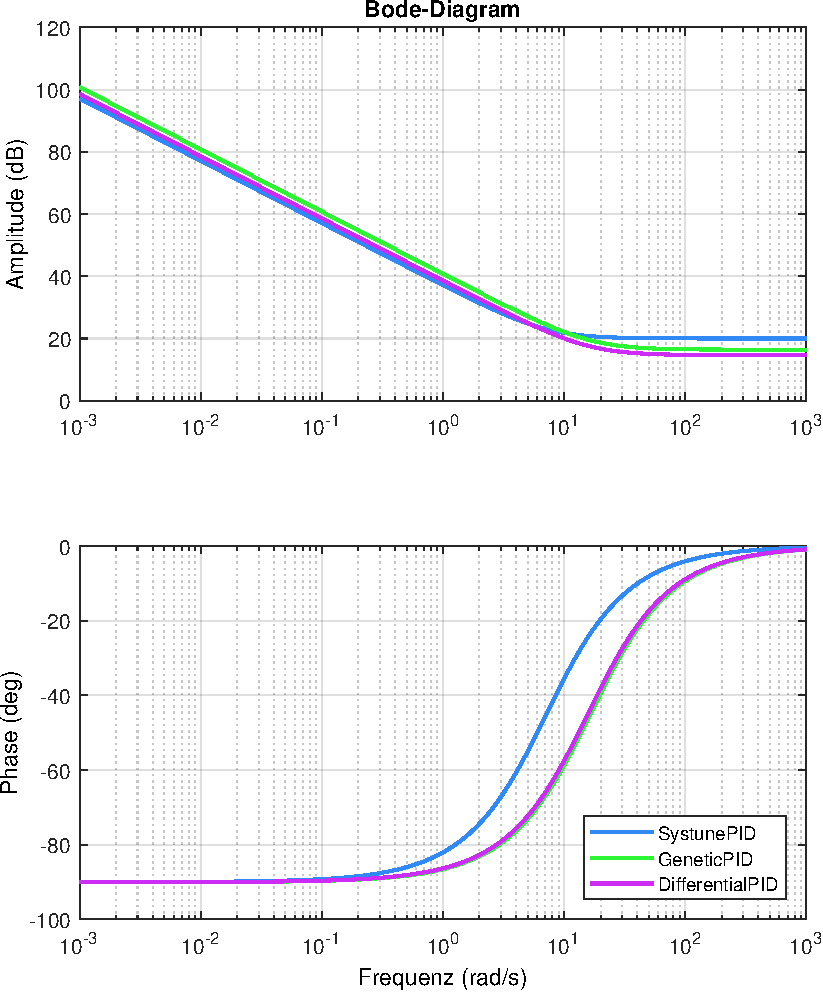
\includegraphics[width=\linewidth]{images/SimpleMotor/CombinedMethodes_PIDBode.pdf}
        \caption{Bode-Diagramm der optimierten Regler}
        \label{fig:SimpleMotorCombinedMethodes_PIDBode}
    \end{figure}
}


\newpage
\subsection{Frequenzanalyse der optimierten Systeme}
%\horizontalLine
\minipagedOrBelowEachOther
{
    \begin{figure}[H]
        \center
        %\vspace{-1.6cm}
        \includegraphics[width=\linewidth]{images/SimpleMotor/CombinedMethodes_SystemBode.pdf}
        \caption{Bode-Diagramm der optimierten Vorwärts Pfade der einzelnen Systeme}
        \label{fig:SimpleMotorCombinedMethodes_SystemBode}
    \end{figure}
    Das Bode-Diagramm in~\ref{fig:SimpleMotorCombinedMethodes_SystemBode} und das
    Nyquist-Diagramm in~\ref{fig:SimpleMotorCombinedMethodes_SystemLogScaleNyquist} zeigen,
    jeweils die Frequenzgänge der optimierten Vorwärts Pfade der drei Systeme:
    \begin{itemize}
        \item \textcolor{systuneColor}{$PID_{\mathbf{systune}} \cdot MotorSystem$}
        \item \textcolor{geneticColor}{$PID_{\mathbf{genetic}} \cdot MotorSystem$}
        \item \textcolor{differentialColor}{$PID_{\mathbf{differential}} \cdot MotorSystem$}
    \end{itemize}

    Im Bode-Diagramm fällt auf, dass der Regler von \textit{systune} nicht zusätzliche Phase klaut.
    Die beste Rauschunterdrückung bietet jedoch der Regler von Differential Evolution.
    
    
}
{
    \begin{figure}[H]
        \center
        %\vspace{-1.6cm}
        \includegraphics[width=\linewidth]{images/SimpleMotor/CombinedMethodes_SystemLogScaleNyquist.pdf}
        \vspace{-0.18cm}
        \caption{Logarithmisches Nyquist-Diagramm der optimierten Vorwärts Pfade der einzelnen Systeme \cite{matlabScriptNyquistLog}}
        \label{fig:SimpleMotorCombinedMethodes_SystemLogScaleNyquist}
    \end{figure}

    \begin{table}[H]
        \center
        \begin{tabular}{@{}cr@{}}
                \toprule
                \textbf{Phasenreserve}              & \textbf{Wert} \\
                \midrule
                \textcolor{systuneColor}{\textit{Systune}}                          & 90.00 ° \\[0.5ex]
                \textcolor{geneticColor}{Genetisch}                        & 80.83 ° \\[0.5ex]
                \textcolor{differentialColor}{Differential Evolution}           & 79.97 ° \\[0.5ex]
                \hline
                \textbf{Verstärkungsreserve}              &  \\
                \hline
                \textcolor{systuneColor}{\textit{Systune}}                          & Inf dB \\[0.5ex]
                \textcolor{geneticColor}{Genetisch}                        & Inf dB \\[0.5ex]
                \textcolor{differentialColor}{Differential Evolution}           & Inf dB \\[0.5ex]
                \bottomrule
        \end{tabular}
        \caption{Reserven optimierten Systeme}
        \label{tab:SimpleMotorCombinedMethodes_AnalyzedData}
    \end{table}
}


\newpage
\subsection{Stabilitätsanalyse der optimierten Systeme}
\subsubsection{Sensitivität}
\begin{figure}[H]
    %\vspace{-1.6cm}
    \includegraphics[width=\linewidth]{images/SimpleMotor/CombinedMethodes_Sensitivity.pdf}
    \caption{Sensitivität der optimierten Systeme}
    \label{fig:SimpleMotorCombinedMethodes_Sensitivity}
\end{figure}
\minipagedOrBelowEachOther
{
    Das Sensitivitäts-Diagramm in \ref{fig:SimpleMotorCombinedMethodes_Sensitivity} zeigt,
    für alle drei Systeme einen ähnlichen Verlauf. Keine Überhöhung, was ein gutes Stabilitätsverhalten andeutet.
    Nicht auf den ersten Blick ersichtlich ist jedoch, dass die Systeme sehr empfindlich auf Totzeiten reagieren.
    Dies ist in Abschnitt \fullref{sec:SimpleMotorStabilityDelayMarginsPlot} dargestellt.
}
{

}

\horizontalLine
\begin{figure}[H]
    \subsubsection{Phasen- \& Verstärkungsreserve Diagramme der optimierten Systeme}
    \begin{minipage}[t]{0.32\textwidth}
        \begin{figure}[H]
            %\vspace{-1.6cm}
            \includegraphics[width=\linewidth]{images/SimpleMotor/SystuneStabilityPhaseMarginsPlot.pdf}
            \caption{Phasen- \& Verstärkungsreserve des mit \textit{systune} optimierten Systems}
            \label{fig:SimpleMotorSystuneStabilityPhaseMarginsPlot}
        \end{figure}
    \end{minipage}
    \hfill
    \begin{minipage}[t]{0.32\textwidth}
        \begin{figure}[H]
            %\vspace{-1.6cm}
            \includegraphics[width=\linewidth]{images/SimpleMotor/GeneticStabilityPhaseMarginsPlot.pdf}
            \caption{Phasen- \& Verstärkungsreserve des mit Genetic optimierten Systems}
            \label{fig:SimpleMotorGeneticStabilityPhaseMarginsPlot}
        \end{figure}
    \end{minipage}
    \hfill
    \begin{minipage}[t]{0.32\textwidth}
        \begin{figure}[H]
            %\vspace{-1.6cm}
            \includegraphics[width=\linewidth]{images/SimpleMotor/DifferentialStabilityPhaseMarginsPlot.pdf}
            \caption{Phasen- \& Verstärkungsreserve des mit Differential Evolution optimierten Systems}
            \label{fig:SimpleMotorDifferentialStabilityPhaseMarginsPlot}
        \end{figure}
    \end{minipage}


\minipagedOrBelowEachOther
{
    Die drei Diagramme in
\ref{fig:SimpleMotorSystuneStabilityPhaseMarginsPlot}, 
\ref{fig:SimpleMotorGeneticStabilityPhaseMarginsPlot} und 
\ref{fig:SimpleMotorDifferentialStabilityPhaseMarginsPlot}
    zeigen die detaillierten Stabilitätsreserven als Kombination von Verstärkung und 
    konstanter Phasenverschiebung.
    Wie diese Diagramme zu lesen sind, ist in folgendem Kapitel erklärt:\\
\fullref{sec:StabilitaetsPhaseMarginPlot}
}
{
    Das System welches mit \textit{systune} optimiert wurde, zeigt eine grössere Fläche indem das System stabil bleibt.
    Dies deutet darauf hin, dass dieses System robuster gegenüber Verstärkungsänderungen und Phasenverschiebungen ist.
}
\end{figure}



\newpage
\begin{figure}[H]
    \subsubsection{Totzeit- \& Verstärkungsreserve Diagramme der optimierten Systeme}
    \label{sec:SimpleMotorStabilityDelayMarginsPlot}
    \begin{minipage}[t]{0.32\textwidth}
        \begin{figure}[H]
            %\vspace{-1.6cm}
            \includegraphics[width=\linewidth]{images/SimpleMotor/SystuneStabilityDelayMarginsPlot.pdf}
            \caption{Totzeit- \& Verstärkungsreserve des mit \textit{systune} optimierten Systems}
            \label{fig:SimpleMotorSystuneStabilityDelayMarginsPlot}
        \end{figure}
    \end{minipage}
    \hfill
    \begin{minipage}[t]{0.32\textwidth}
        \begin{figure}[H]
            %\vspace{-1.6cm}
            \includegraphics[width=\linewidth]{images/SimpleMotor/GeneticStabilityDelayMarginsPlot.pdf}
            \caption{Totzeit- \& Verstärkungsreserve des mit Genetic optimierten Systems}
            \label{fig:SimpleMotorGeneticStabilityDelayMarginsPlot}
        \end{figure}
    \end{minipage}
    \hfill
    \begin{minipage}[t]{0.32\textwidth}
        \begin{figure}[H]
            %\vspace{-1.6cm}
            \includegraphics[width=\linewidth]{images/SimpleMotor/DifferentialStabilityDelayMarginsPlot.pdf}
            \caption{Totzeit- \& Verstärkungsreserve des mit Differential Evolution optimierten Systems}
            \label{fig:SimpleMotorDifferentialStabilityDelayMarginsPlot}
        \end{figure}
    \end{minipage}


\minipagedOrBelowEachOther
{
    Die drei Diagramme in 
\ref{fig:SimpleMotorSystuneStabilityDelayMarginsPlot}, 
\ref{fig:SimpleMotorGeneticStabilityDelayMarginsPlot} und 
\ref{fig:SimpleMotorDifferentialStabilityDelayMarginsPlot}
    zeigen die detaillierten Stabilitätsreserven aus der Kombination von Verstärkung und 
    Totzeit.
Wie diese Diagramme zu lesen sind, ist in folgendem Kapitel erklärt:\\
\fullref{sec:StabilitaetsDelayMarginPlot}
}
{
    Auch wenn die Verstärkungsreserven und Phasenreserven der drei Systeme scheinbar sehr gut sind,
    reagieren die Systeme auf Kombinationen von Totzeit und Verstärkungsänderungen sehr empfindlich.
    Bereits eine kleine Totzeit von ca. 4ms führt bei allen drei Systemen zu Instabilität.
    Die Systeme verhalten sich also nicht sehr robust.\\


    Besonders das mit \textit{systune} optimierte System, welches in den obigen Analysen doch die besten Ergebnisse,
    was Robustheit anbelangt, gezeigt hat, reagiert auf Totzeiten am empfindlichsten und wird bereits bei einer Totzeit von ca. 2.5ms instabil.
}
\end{figure}
\newpage




\section{\textit{Systune} am Motor mit Schwungmasse}
\label{sec:SystuneAmMotorMitSchwungmasse}
Wie bereits im Beispiel \fullref{sec:SystuneAmDCMotor} beschrieben, 
wird hier der gleiche Ablauf, aber diesmal für das Motor-mit-Schwungmasse-System, durchgeführt.
Deshalb wird darauf verzichtet jeden Schritt in Detail erneut zu beschreiben.
Das komplette MATLAB-Skript kann im GitHub Repository \cite{baRepository} eingesehen werden.


\subsection{Regelkreis Definieren}
\minipagedOrBelowEachOther
{
    %\vspace{0.8cm}
    Der verwendete Regelkreis ist im Kapitel\\
    ~\fullref{sec:MotorMitSchwungmasseModellidentifikation} genauer beschrieben.
	Da der Regelkreis für \textit{systune} linear sein muss, werden die nichtlinearen Sättigungsblöcke vernachlässigt und 
    erst beim Testen des optimierten Systems wieder berücksichtigt.
}{
	%\centering
    \begin{figure}[H]
    \centering
    \begin{tikzpicture}[>=latex', scale=1]
    % Manually set bounding box
    \useasboundingbox (0,0) rectangle (8,-1);
    \newcommand{\labeloffset}{0.2}
    % Draw grid
    %\draw[step=1cm,gray,very thin] (0,0) grid (10,10);

    \newcommand{\plantSys}{M=$|$w$|$=M};
    \newcommand{\controllerSys}{$\mathbf{PID}$};
    
    % Draw blocks
    \sumNode{sum}{0.5,0};

    \blockNode{controller}{2,0}{\controllerSys};
    \connectionNode{analysisPoint}{0.5,-1};
    \gainNode[east]{u1gain}{$(controller.east) + (1,0)$}{300};
    \blockNode{plant}{$(u1gain.east) + (1.7,-0.25)$}{\plantSys};

    % Draw connections
    \connect[label={-0.6,0}{$\mathbf{r}$}              ]{(-0.2,0)             (sum.west)          }{->};
    \connect[label={-0.5,\labeloffset}{$\mathbf{e}$}   ]{(sum.east)        (controller.west)   }{->};
    %\connect[label={-0.5,\labeloffset}{$\mathbf{u_{Out}}$}]{(controller.east) (analysisPoint.center)}{-};
    \connect{(controller.east) (u1gain.west)   }{->};
    \connect[label={-0.3,\labeloffset}{$\mathbf{u_{1}}$}]{(u1gain.east) ($(plant.west) + (0,0.25)$)   }{->};
    %\connect[label={0, \labeloffset}{$\mathbf{u_{AP}}$}]{(analysisPoint.center) ($(analysisPoint.center) + (0, 0.5)$)   }{->, dashed};
    \connectionNode{output}{$(plant.east) + (0.5,-0.25)$};
    \connect[label={0.2,0}{$\mathbf{y_2}$}               ]{\vectorAdd{plant.east}{0,-0.25} (output.center) \vectorAdd{output}{0.5,0}}{->};
    \connect[label={0.2,0}{$\mathbf{y_1}$}               ]{\vectorAdd{plant.east}{0,0.25} \vectorAdd{plant.east}{1,0.25}}{->};
    \connect[label={-0.3,-\labeloffset}{$\mathbf{u_2}$}  ]{\vectorAdd{plant.west}{-0.5,-0.25} \vectorAdd{plant.west}{0,-0.25}}{->};
    \connect[label={0, \labeloffset}{$\mathbf{u_{AP}}$}]{(analysisPoint.center) ($(analysisPoint.center) + (-0.5, 0)$)   }{->, dashed};

    \feedback[sign={-0.3,-0.1}              ]{output.center}{-0.5}{sum.south}{->};
\end{tikzpicture}
    \caption{Regelkreis des Motors mit Schwungmasse}
    \label{fig:MotorMitSchwungmasseTikzDiagram_systune}
    \end{figure}
}



\horizontalLine
\subsection{Optimierungsziele definieren}
Bei den optimierungszielen können verschiedene Kriterien verwendet werden. 
In diesem Beispiel werden drei Ziele definiert:
\begin{itemize}
    \item \textbf{Step-Tracking}: Das System soll der Sprungantwort eines PT2-Systems folgen.
    \item \textbf{Overshoot}: Das Überschwingen soll begrenzt werden.
    \item \textbf{Phasen- und Verstärkungsreserve}: Die Stabilitätsreserven sollen eingehalten werden.
\end{itemize}

\subsubsection{TuningGoal.StepTracking \cite{matlabTuningGoals_StepTracking}}
\minipagedOrBelowEachOther
{
    Das Step-Tracking Ziel sorgt dafür, dass das System einer vordefinierten Sprungantwort folgt.
    Dafür wird ein PT2-System als Referenz verwendet.
    In diesem Beispiel wird eine Zeitkonstante von $\tau = 0.2$ und eine Dämpfung von $D = 1$ verwendet.
    Die Wahl dieser Parameter entspricht approximativ den Parametern aus der Impulsantwort welche bei der 
    Systemidentifikation in Kapitel~\fullref{sec:MotorMitSchwungmasseModellidentifikation} ermittelt wurde.
}{
	\begin{equation}
        H_{\mathbf{ref}}(s) = \frac{1}{\tau^2 \cdot s + 2 \cdot D \cdot \tau \cdot s + 1} \quad \text{mit} \quad \tau = 0.2, D = 1
    \end{equation}
}
\begin{matlabcode}{Definition des Step-Tracking Ziels}{lst:motorMitSchwungmasseStepTrackingZielDefinition_systune}
pt2T = 0.2;
pt2D  = 1;
pt2Step = tf([1],[pt2T*pt2T 2*pt2D*pt2T 1]);
TR1 = TuningGoal.StepTracking('r', 'y2', pt2Step);  
\end{matlabcode}




\subsubsection{TuningGoal.Overshoot \cite{matlabTuningGoals_Overshoot}}
Das Overshoot Ziel begrenzt das Überschwingen des Systems.
Ziel ist es, vom Referenzsignal $r$ zur Ausgangsgrösse $y2$ nicht mehr als 10\% Überschwingen zuzulassen.

\begin{matlabcode}{Definition des Overshoot Ziels}{lst:motorMitSchwungmasseOvershootZielDefinition_systune}
TR2 = TuningGoal.Overshoot('r', 'y2', 10);  
\end{matlabcode}




\subsubsection{TuningGoal.Margins \cite{matlabTuningGoals_Margins}}
\minipagedOrBelowEachOther{
    Das Margins-Ziel sorgt dafür, 
    dass die Stabilitätsreserven eingehalten werden.
    In diesem Beispiel sollen eine Phasenreserve von mindestens 45° und 
    eine Verstärkungsreserve von mindestens 6dB eingehalten werden.
}{
    Der angegebene Analysis-Point 'uAP' steht für den Teil des Feedbacks, 
    welcher für die Stabilitätsanalyse aufgetrennt wird 
    um die Messung der Phasen- und Verstärkungsreserven zu ermöglichen.
}


\begin{matlabcode}{Definition des Margins Ziels}{lst:motorMitSchwungmasseMarginsZielDefinition_systune}
TR4 = TuningGoal.Margins('uAP', 6, 45);
\end{matlabcode}


\subsubsection{Optimierungsziele kombinieren}
\begin{matlabcode}{Kombinieren der Optimierungsziele}{lst:motorMitSchwungmasseOptimierungszieleKombinieren_systune}
targetSoftGoals = [TR1  TR2]; % Step-Tracking und Overshoot
targetHardGoals = [TR4];      % Phasen- und Verstärkungsreserven
\end{matlabcode}





\newpage
\subsection{Regler extrahieren}
Nach der Optimierung kann der optimierte Regler aus dem Gesamtsystem extrahiert werden.
\begin{matlabcode}{Regler extrahieren}{lst:DCMotorReglerExtrahieren_systune}
    controllerSysTuned = getBlockValue(sysTuned, 'controllerSys');
    disp(controllerSysTuned);
\end{matlabcode}
\begin{matlabcode}{Optimierter Regler}{lst:motorMitSchwungmasseControllerSysTunedOutput_systune}
  pid with properties:

              Kp: -0.4108
              Ki: -4.6926e-08
              Kd: -0.7332
              Tf: 0.0802
              ...
\end{matlabcode}



\horizontalLine
\subsection{Optimierung auswerten}
Die Ziele wurden gut erreicht, da alle unter 1 liegen.
\begin{matlabcode}{TuningGoals Auswertung}{lst:motorMitSchwungmasseTuningGoalsAuswertungOutput_systune}
Final soft objective: 0.3065 (< 1 is good)
Final soft objective: 0.6893 (< 1 is good)
Final hard objective: 0.6066 (< 1 is good)

%=== Performance Comparison ===
%                  Initial    Tuned
%Rise Time:        NaN s    0.660 s
%Settling Time:    NaN s    1.180 s
%Overshoot:        NaN %    0.31 %
%
%Gain Margin:      Na  dB   19.83 dB
%Phase Margin:      <0 °    75.71 °
\end{matlabcode}






\newpage
\subsubsection{Step-Tracking Ergebnis visualisiert}
\begin{matlabcode}{Step-Tracking Diagramm}{lst:motorMitSchwungmasseOptimierungsanalyseOutput_systuneStepTracking}
viewGoal(targetSoftGoals(1), sysTuned);
\end{matlabcode}
\minipagedOrBelowEachOther
{
    \vspace{1cm}
    Das Diagramm in~\ref{fig:motorMitSchwungmasseSystuneTuningGoalStepTrackingResult} zeigt die Sprungantwort des 
    optimierten Systems. Die Kurve mit dem Namen \textit{Desired} entspricht der gewünschten Sprungantwort,
    die durch das Step-Tracking Ziel definiert wurde: 
    $H_{\mathbf{ref}}(s) = \frac{1}{\tau^2 \cdot s + 2 \cdot D \cdot \tau \cdot s + 1} \quad \text{mit} \quad \tau = 0.2, D = 1$.
    In blau ist die Sprungantwort des optimierten Systems dargestellt.
    Diese deckt sich hauptsächlich kurz nach dem Start sehr gut mit der gewünschten Sprungantwort.
}{
	%\centering
   % \vspace{-1cm}
    \begin{figure}[H]
        %\centering
        \includegraphics[width=\linewidth]{images/MotorMitSchwungmasse/SystuneTuningGoalSoft_1.pdf}
        \caption{Step-Tracking Optimierungsergebnis mit \textit{systune} am Motor mit Schwungmasse}
        \label{fig:motorMitSchwungmasseSystuneTuningGoalStepTrackingResult}
    \end{figure}
}

\horizontalLine
\subsubsection{Overshoot Ergebnis visualisiert}
\begin{matlabcode}{Overshoot Diagramm}{lst:motorMitSchwungmasseOptimierungsanalyseOutput_systuneOvershoot}
viewGoal(targetSoftGoals(2), sysTuned);
\end{matlabcode}
\minipagedOrBelowEachOther
{
    \vspace{0.6cm}
	Das Diagramm in~\ref{fig:motorMitSchwungmasseSystuneTuningGoalOvershootResult} zeigt den Frequenzgang des optimierten geschlossenen Systems.
    Der orange Bereich stellt den Tiel der Verstärkung dar, welcher grösser als die erlaubten 10\% Überschwingen ist.
    Die blaue Kurve zeigt die Verstärkung des optimierten Systems, diese ist im gesamten Frequenzbereich unterhalb der
    10\% Grenze, was zeigt, dass das Overshoot Ziel erfolgreich erfüllt wurde.
}{
	%\centering
    \begin{figure}[H]
        %\vspace{-1cm}
        \includegraphics[width=\linewidth]{images/MotorMitSchwungmasse/SystuneTuningGoalSoft_2.pdf}
        \caption{Overshoot Optimierungsergebnis mit \textit{systune} am Motor mit Schwungmasse}
        \label{fig:motorMitSchwungmasseSystuneTuningGoalOvershootResult}
    \end{figure}
}

\newpage
\subsubsection{Phasen- und Verstärkungsreserven Ergebnis visualisiert}
\begin{matlabcode}{Phasen- und Verstärkungsreserven Diagramm}{lst:motorMitSchwungmasseOptimierungsanalyseOutput_systunePhaseAndGainMargin}
viewGoal(targetHardGoals(1), sysTuned);
\end{matlabcode}
\minipagedOrBelowEachOther
{
    %\centering
    \begin{figure}[H]
        \centering
        \includegraphics[width=\linewidth]{images/MotorMitSchwungmasse/SystuneTuningGoalHard_1.pdf}
        \caption{Phasen- und Verstärkungsreserven Optimierungsergebnis mit \textit{systune} am Motor mit Schwungmasse}
        \label{fig:motorMitSchwungmasseSystuneTuningGoalPhaseAndGainMarginResult}
    \end{figure}
    %\vspace{-1cm}
	Das Diagramm in \ref{fig:motorMitSchwungmasseSystuneTuningGoalPhaseAndGainMarginResult} zeigt die Verstärkungs- und 
    Phasenreserven des optimierten geschlossenen Systems.
    Die blaue Kurve zeigt jeweils den Verstärkungsreserven (oben) und die Phasenreserve (unten) des optimierten Systems.
    Beide Kurven liegen über den geforderten Mindestreserven (oranger Bereich), 
    was zeigt, dass das Margins-Ziel erfolgreich erfüllt wurde.  

    \vspace{0.3cm}
    Mehr Informationen darüber, wie die Optimierungsergebnisse visualisiert werden,
    ist in der MATLAB Dokumentation zu den Tuning-Goals beschrieben. \cite{matlabTuningGoals_VisualizeTuningGoals}
}{
	%\centering
    \begin{figure}[H]
        \centering
        \includegraphics[width=0.838\linewidth]{images/MotorMitSchwungmasse/SystuneStabilityDelayMarginsPlot.pdf}
        \caption{Totzeit \& Verstärkungsreserve Diagramm des optimierten Systems}
        \label{fig:motorMitSchwungmasseSystuneStabilityMarginsPlot}
    \end{figure}

    Das von MATLAB generierte Diagramm kann verwirren und ist nicht einfach zu interpretieren.
    Eine bessere Darstellung über die resultierten Phasen- und Verstärkungsreserven ist in
    \ref{fig:motorMitSchwungmasseSystuneStabilityMarginsPlot} zu sehen.
    Wie diese Abbildung interpretiert wird, ist in folgendem Kapitel erklärt:\\
\fullref{sec:StabilitaetsDelayMarginPlot}


    Das Diagramm zeigt, dass das System über eine grosse Phasenreserve
    verfügt. Das zeigt sich durch die Toleranz der möglichen Totzeiten mit bis zu 0.6s
    bei einer Verstärkung von 1.
    Ausserdem besitzt das System eine gute Verstärkungsreserve mit bis zu 20dB\\
    (Verstärkungsfaktor = 10).
}
\newpage

%\minipagedOrBelowEachOther
%{
%    
%}{
%	
%}



%\horizontalLine
\subsection{Optimierten Regler am realen System testen}

%\subsubsection{Reales System Resultat}
\begin{figure}[H]
    \centering
    \includegraphics[width=\linewidth]{images/MotorMitSchwungmasse/Systune_realResult.pdf}
    \caption{Antwort auf Stimulation des optimierten Reglers am Motor mit Schwungmasse, mit dem durch \textit{systune} optimierten PID-Regler}
    \label{fig:MotorMitSchwungmasseSystune_realResult}
\end{figure}

\minipagedOrBelowEachOther
{
    Für den Test am realen Prozess sind im Simulink Modell unterschiedliche Sollwerte vorbereitet. 
    Auch die Sättigungen sind wieder eingebaut.
    Da der PID-Regler am Ausgang einen Sättigungsblock besitzt, entsteht das Problem des Integrator Windups.
    Die \textit{Clamping} Anti-Windup Methode wird verwendet, da diese keinen weiteren Tuning-Parameter erzeugt.
    \textit{Systune} kann leider keinen Anti-Windup Tuning-Parameter optimieren.
}
{
    Der Regler verstärkt an seinem Ausgang $u1$ das Messrauschen des Encoders, welches zu starken 
    Stromschwankungen am Motoreingang führen. 
    Es ist zu erkennen, dass der Ist-Winkel $y2$, sobald die Störgrösse dazu geschaltet wird, davon driftet.
    Der Regler besitzt deshalb keine guten Eigenschaften um Störgrössen zu kompensieren.
}
\newpage
\section{GA am Motor mit Schwungmasse}

% Commands already define in GA am DC-Motor
%\newcommand{\individuumI}{\overrightarrow{I_{\mathbf{i}}}}
%\newcommand{\funcGOfk}[1]{\mathFunction{g_\mathbf{#1}}{\individuumI,k}}
%\newcommand{\funcGOf}[1]{\mathFunction{g_\mathbf{#1}}{\individuumI}}

\minipagedOrBelowEachOther
{
    Weil der \gls{GA} kein MATLAB voraussetzt, ist diese Methode auch ohne MATLAB implementiert worden.
	Das hat den Vorteil, dass ein System auch ohne MATLAB Lizenz optimiert werden kann.
}
{
	Die Funktionsweise des GA ist im Kapitel\\
	\fullref{sec:Description_GenetischerAlgorithmus} beschrieben.
	
}

\subsection{System Definieren}
\begin{figure}[H]
    \centering
    \begin{tikzpicture}[auto, node distance=2cm,>=latex', scale=1]
    \newcommand{\labeloffset}{0.2}
    % Draw grid
    %\draw[step=1cm,gray,very thin] (0,0) grid (10,10);
    
    % Draw blocks
    \sumNode{sum}{1,0};

    %\saturationBlockNode{saturation1}{-1, 0}{-10}{10};
    \saturationBlockNode{saturation3}{4.5, 2}{-10}{10};
    \blockNode{controller}{2.5,0}{$PID$};
    \saturationBlockNode{saturation2}{4.5,0}{-10}{10};
    \gainNode[east]{u1gain}{$(saturation2.east) + (1,0)$}{300};
    \gainNode[east]{u2gain}{$(saturation3.east) + (1,0)$}{300};
    \blockNode{plant}{$(u1gain.east) + (2,-0.25)$}{M=$|$w$|$=M};

    % Draw connections
    %\connect{(-2.5,0)             (saturation1.west)          }{->};
    \connect[label={-3.6,\labeloffset}{$\mathbf{d}$}              ]{(0,2)             (saturation3.west)          }{->};
    \connect[label={-0.5,\labeloffset}{$\mathbf{r}$}              ]{(0,0)             (sum.west)          }{->};
    \connect[label={-0.5,\labeloffset}{$\mathbf{e}$}   ]{(sum.east)        (controller.west)   }{->};
    \connect{(controller.east) (saturation2.west)   }{->};
    
    \connect{(saturation2.east) (u1gain.west)        }{->};
    \connect[label={-0.25, \labeloffset}{$\mathbf{u_{1}}$}   ]{(u1gain.east) ($(plant.west) + (0, 0.25)$)        }{->};
    \connectionNode{output}{$(plant.east) + (0.5,-0.25)$};
    \connect[label={0.2,0}{$\mathbf{y_{2}}$}               ]{\vectorAdd{plant.east}{0,-0.25} (output.center) \vectorAdd{output}{0.5,0}}{->};
    \connect[label={0.2,0}{$\mathbf{y_{1}}$}               ]{\vectorAdd{plant.east}{0,0.25} \vectorAdd{plant.east}{1,0.25}}{->};
    \connect{(saturation3.east) (u2gain.west)}{->};
    \connect[label={-0.25, -\labeloffset}{$\mathbf{u_{2}}$}]{(u2gain.east) ($(plant.west) + (-0.6, 2.25)$) ($(plant.west) + (-0.6, -0.25)$) ($(plant.west) + (0, -0.25)$)}{->};

    \feedback[sign={-0.3,-0.1}              ]{output.center}{-1}{sum.south}{->};
\end{tikzpicture}
    \caption{Regelkreis Motor mit Schwungmasse}
    \label{fig:MotorMitSchwungmasseTikzDiagram_genetic}
\end{figure}
In der C++ Anwendung werden die Teilsysteme objektorientiert implementiert und anschliessend 
als ein gesamtheitliches Objekt zusammengeführt und verbunden.
Der Kernteil der Implementierungslogik spielt sich dabei in den Update-Funktionen der jeweiligen Teilsysteme ab.
Aufgrund des Codes-Umfangs werden deshalb in den nachfolgenden Unterkapiteln nur die Update-Funktionen gezeigt.


\horizontalLine
\subsubsection{Motor definieren}
Die Implementierung im C++ Code ist auf der Grundlage der Modellidentifikation des Systems im Kapitel
\fullref{sec:MotorMitSchwungmasseModellidentifikation} durchgeführt worden.
Die dazugehörige C++ Implementierung ist unter
\fullref{lst:MotorMitSchwungmasseDefinitionCPP} zu finden.
%\minipagedOrBelowEachOther
%{
%	
%}{
%	
%}



\horizontalLine
\subsubsection{PID-Regler definieren}
Der PID-Regler wurde bereits im Kapitel \fullref{sec:ErweiterterPIDRegler} beschrieben und 
auch die C++ Implementierung wird dort aufgeführt. Deshalb wird hier nicht weiter darauf eingegangen.




\horizontalLine
\subsubsection{Alle Teilsysteme verbinden}
\begin{cppcode}{Update-Funktion des Gesamtsystems im Code}{lst:MotorMitSchwungmasseRegelkreisCPP}
// Update Funktion des Gesamtsystems im C++ Code. class TestSystem
void update(double deltaTime) override
{
	double y = m_motorWithMass.getOutputs()[1];	// y(t)
    double measurementNoise = AutoTuner::Solver::getRandomDouble(-1, 1) * 0.1;
    m_errorValue = m_referenceValue - y + measurementNoise;				// e(t) = r(t) - y(t)

    m_pidController.setInput(m_errorValue);

	m_pidController.update(deltaTime);
    m_pidOutputValue = m_pidController.getOutput();
    m_motorWithMass.setInputSignal(0, m_pidOutputValue);
    m_motorWithMass.setInputs(1, m_disturbanceValue);
    m_motorWithMass.update(deltaTime);
}
\end{cppcode}
\minipagedOrBelowEachOther{
	Wie im Code ersichtlich ist, wird dem System ein zusätzliches Messrauschen hinzugefügt.
	Dieses begünstigt die Eigenschaft der Rauschunterdrückung des Reglers durch die Bewertungsteilfunktion
	$\mathFunction{g_\mathbf{1}}{\individuumI}$ (Stellwertänderungsrate).
}{

}


\newpage
\subsection{Optimierungsziele definieren}
\begin{figure}[H]
    \centering
    \includegraphics[width=\linewidth]{images/MotorMitSchwungmasse/Stimuli.pdf}
    \caption{Anregungssignale für die Systemsimulation}
    \label{fig:MotorMitSchwungmasseStimuli}
\end{figure}
Um die Bewertungsfunktion zu definieren wird eine zeitliche Simulation des Systems benötigt.
Dazu wird ein vordefiniertes Anregungssignal verwendet.
Das Anregungssignal besteht aus $r$ (Ziel-Winkel) und $d$ (Störungsmoment).


\newpage
\begin{table}[H]
\centering
\begin{tabular}{@{}clrc@{}}
		\toprule
		\textbf{Symbol} & \textbf{Beschreibung} & \textbf{Wert} & \textbf{Einheit} \\
		\midrule
		$Ts$                & Abtastzeit &0.01& s\\[0.5ex]
		$t_\mathbf{start}$  & Startzeit &0& s\\[0.5ex]
		$t_\mathbf{end}$    & Endzeit &50& s\\[0.5ex]
		$u_\mathbf{satHigh}$   & Obere Sättigungsgrenze der Stellgrösse &10& \\[0.5ex]
		$u_\mathbf{satLow}$   & Untere Sättigungsgrenze der Stellgrösse &-10& \\[0.5ex]
		%$N$                 & Anzahl Individuen in der Population &30\\[0.5ex]
		$K$                 & Anzahl Zeitschritte in der Simulation & 5000\\[0.5ex]
		$D$				  & Anzahl der Optimierungs-Parameter & 4 & \\[0.5ex]
		$\individuumI$    & \gls{Individuum} $\mathbf{i}$ in der \gls{Population} & $\individuumI \in \mathbb{R}^D$ \\[0.5ex]
		%$\mathFunction{f}{\individuumI}$ & Maximierungs-Fitness-Funktion.& $f(\individuumI) \in \mathbb{R}^{+}$ \\[0.5ex]
		$\mathFunction{g}{\individuumI}$ & Fehler-Minimierungs-Funktion. & $\mathFunction{g}{\individuumI} \in \mathbb{R}$ \\[0.5ex]
		$a_\mathbf{o}$      & Gewichtungsfaktor für das Optimierungsziel $\mathbf{o}$ & $a_\mathbf{o} \in \mathbb{R}^{+_0}$ \\[0.5ex]
		$O$                 & Anzahl Optimierungsziele & 5 \\[0.5ex]
		$\funcGOfk{o}$ & Optimierungsfunktion für das Ziel $\mathbf{o}$ zum Zeitpunkt $k$ & $\funcGOfk{o} \in \mathbb{R}$ \\[0.5ex]
		\bottomrule
\end{tabular}
\caption{Symbole für die Simulation am Motor mit Schwungmasse}
\end{table}


Für die Abtastzeit $Ts$ wurde ein realistischer Wert von 10ms gewählt.\\


\minipagedOrBelowEachOther
{
	Die Anzahl Zeitschritte $K$ wird aus der Abtastzeit $T_\mathbf{s}$ und 
	dem Simulationszeitraum $[t_\mathbf{start}, t_\mathbf{end}]$ berechnet.  
}{
	\centering
    \begin{equation}
		K = \frac{t_\mathbf{end}-t_\mathbf{start}}{T_\mathbf{s}}
	\end{equation}
}

\horizontalLine

\minipagedOrBelowEachOther
{
	Der \gls{GA} ist für \gls{Maximierungsproblem}e ausgelegt. 
	Für diese Anwendung wäre es aber sinnvoller die Optimierungsziele als \gls{Minimierungsproblem}e zu formulieren.
	Es gibt jedoch eine Möglichkeit zur Umrechnung von \gls{Minimierungsproblem}en in Maximierungsprobleme.
	Dies ist im Kapitel \fullref{sec:Description_GenetischerAlgorithmus_FitnessFunction_TransformationSteps} beschrieben.
	Dank dieser Umrechnung können die Optimierungsziele als Minimierungsproblem formuliert werden.

	Die Fehler-Minimierungs-Funktion $\mathFunction{g}{\individuumI}$
	wird aus mehreren Teilsummen zusammengesetzt. Die Teilsummen bewerten verschiedene Aspekte des Regelverhaltens.
	Allgemein lässt sich die Fehler-Minimierungs-Funktion $\mathFunction{g}{\individuumI}$ wie in der 
\ref{form:MotorMitSchwungmasseGeneticAlgorithmErrorMinimizationFunction} darstellen.
}{
	
    \begin{equation}
		\label{form:MotorMitSchwungmasseGeneticAlgorithmErrorMinimizationFunction}
		\mathFunction{g}{\individuumI} = 
		\frac{1}{K} \cdot \sum_{k=0}^{K-1}\bigg(
				\sum_{o=0}^{O-3}\Big( 
					a_\mathbf{o} \cdot \funcGOfk{o}
				\Big)
			\bigg) + a_\mathbf{3} \cdot \funcGOf{\mathbf{3}}
			  + a_\mathbf{4} \cdot \funcGOf{\mathbf{4}}
	\end{equation}
	
	\begin{itemize}
		\item $\frac{1}{K}$ dient zur Normierung der Fehlerbewertung auf die Anzahl der Zeitschritte.
		\item $\sum_{k=0}^{K-1}$ summiert die Fehlerbewertung über alle Zeitschritte der Simulation.
		\item $\sum_{o=0}^{O-3}\left( 
					a_\mathbf{o} \cdot \funcGOfk{o}
				\right) $ summiert die gewichteten Optimierungsziele $\funcGOfk{o}$ für den Zeitschritt $k$.
		\item $a_\mathbf{3} \cdot \funcGOf{\mathbf{3}}$ bewertet die Verstärkungsreserve des Systems.
		\item $a_\mathbf{4} \cdot \funcGOf{\mathbf{4}}$ bewertet die Phasenreserve des Systems.
	\end{itemize}

	$\funcGOf{\mathbf{3}}$ und $\funcGOf{\mathbf{4}}$ 
	werden nicht über die Zeitschritte während der Simulation summiert, 
	da sie nicht abhängig von der Laufzeit der Simulation sind, 
	sondern approximiert im Frequenzbereich berechnet werden.
}







%\begin{equation}
%	\mathFunction{g}{\individuumI} = 
%	\frac{1}{t_\mathbf{end}-t_\mathbf{start}}\sum_{k=0}^{K}(
%		a_\mathbf{1} \cdot \mathFunction{g_\mathbf{1}}{k} + 
%		a_\mathbf{2} \cdot \mathFunction{g_\mathbf{2}}{k}
%		)
%\end{equation}

%\horizontalLine



\newpage
Folgende Optimierungsziele wurden bereits im Kapitel 
~\fullref{sec:Description_GenetischerAlgorithmus_FitnessFunction_OptimizationGoals_SimpleMotor} 
im Zusammenhang mit dem DC-Motor beschrieben und werden hier deshalb nicht nochmals erklärt:
\begin{itemize}
    \item $\funcGOfk{\mathbf{0}}$: Absoluter Regelungsfehler aber ohne Sättigungsbedingung 
    \item $\funcGOfk{\mathbf{1}}$: Stellwertänderungsrate
    \item $\funcGOfk{\mathbf{2}}$: Positives Überschwingen unterdrücken
\end{itemize}

\horizontalLine
\subsubsection{$\funcGOf{\mathbf{3}}$: Verstärkungsreserve}
\minipagedOrBelowEachOther
{
	$\funcGOf{\mathbf{3}}$ bewertet die quadratische Abweichung der Verstärkungsreserve des Systems
    von dem gewünschten Wert von 2. 	      
}{
	Diese Bewertung wurde für den Test deaktiviert ($a_\mathbf{3} = 0$), 
    da die Optimierung dem System von sich aus eine weitaus bessere Verstärkungsreserve verpasst als gefordert und so
    wie die Bewertung formuliert ist, würde der \gls{Solver} versuchen, die Verstärkungsreserve wieder zu verschlechtern.
}
\vspace{0.1cm}
\horizontalLine
\subsubsection{$\funcGOf{\mathbf{4}}$: Phasenreserve}
\minipagedOrBelowEachOther
{
	$\funcGOf{\mathbf{4}}$ bewertet die quadratische Abweichung der Phasenreserve des Systems
    von dem gewünschten Wert von 90°.
	Die Bewertung wird erst ab Epoche 100 durchgeführt, damit der Algorithmus
	zuerst eine grobe Lösung finden kann, bevor die Stabilitätskriterien berücksichtigt werden.
	Die Frequenzanalyse wird mit dem nicht linearisierten System im Zeitbereich durchgeführt.
	Zu Beginn der Simulation ist das System noch instabil, was zu einer falsch berechneten Frequenzanalyse führt 
	und somit ist die Frequenzanalyse erst ab Epoche 100 sinnvoll.
}{
    Es wurde 90° gewählt, weil damit versucht wird, möglichst nah an 90° zu kommen.
    \textit{Systune} hat gezeigt, dass es möglich ist, nah an die 90° zu kommen, ohne das System zu träge zu machen.
}


\horizontalLine
\subsubsection{$\mathFunction{g}{\individuumI}$: Gesamte Fehlerbewertung}
\minipagedOrBelowEachOther
{
	Die Teilbewertungen werden jeweils mit einem \\
	Gewichtungsfaktor $a_\mathbf{o}$ skaliert. Diese müssen vom Anwender\\
	passend gewählt werden, um das gewünschte Verhalten zu erzielen.
	Es ist zu beachten, dass $\funcGOf{\mathbf{4}}$ nicht über 
	die Simulationszeit summiert wird, sondern nur einmal pro Individuum berechnet wird,
	weil sich der Frequenzgang im Verlauf einer Simulationsdurchführung nicht ändert.
}{
	\centering
    \begin{equation}
		\mathFunction{g}{\individuumI} = 
		\frac{1}{K} \cdot \sum_{k=0}^{K-1}\Big(
			a_\mathbf{0} \cdot \funcGOfk{\mathbf{0}} + 
			a_\mathbf{1} \cdot \funcGOfk{\mathbf{1}} +
			a_\mathbf{2} \cdot \funcGOfk{\mathbf{2}}
			\Big)
             +
            a_\mathbf{4} \cdot \funcGOf{\mathbf{4}}
	\end{equation}
}



\newpage
\subsection{Optimierung durchführen}
\begin{figure}[H]
	\center
    %\vspace{-1.6cm}
    \includegraphics[width=\linewidth]{images/MotorMitSchwungmasse/Genetic_SimulationSoftware.png}
    \caption{Software der Systemsimulation für die Optimierung}
    \label{fig:MotorMitSchwungmasseGenetic_SimulationSoftware}
\end{figure}

\minipagedOrBelowEachOther
{
	Wie beim Beispiel mit dem DC-Motor \ref{fig:SimpleMotorGenetic_SimulationSoftware} wird die Optimierung 10-mal durchgeführt
	und bestimmte Hyperparameter werden willkürlich gewählt.

}
{
	Mehr zur Bestimmung der Hyperparameter ist im Kapitel\\
	\fullref{sec:objektivesFazitIterativesTuning} beschrieben.
}

\begin{table}[H]
\centering
\vspace{-0.2cm}
\begin{tabular}{@{}clrc@{}}
		\toprule
		\textbf{Parameter} & \textbf{Beschreibung} & \textbf{Wert} \\
		\midrule
		$D$                 & Anzahl der einzelnen Optimierungsdurchläufe &10\\[0.5ex]
		$N$                 & Anzahl Individuen in der Population &30\\[0.5ex]
		$G$                 & Anzahl Generationen &1000\\[0.5ex]
		$C$                 & Mutations-Wahrscheinlichkeit &0.05\\[0.5ex]
		$\mathFunction{M}{k}$ & Mutationsstärke &$1 \cdot 0.999^{k}$\\[0.5ex]
		Anti-Windup       & Verwendete Anti-Windup Methode & Clamping \\[0.5ex]
		\hline
		\textbf{Optimierungsziele} &  &  & \\[0.5ex]
		$a_\mathbf{0}$     & Absoluter Regelungsfehler &2.8\\[0.5ex]
		$a_\mathbf{1}$     & Stellwertänderungsrate &0.1\\[0.5ex]
		$a_\mathbf{2}$     & Positives Überschwingen &111\\[0.5ex]
        $a_\mathbf{3}$     & Verstärkungsreserve (6dB) &0\\[0.5ex]
        $a_\mathbf{4}$     & Phasenreserve (90°) &99 Ab Epoche 100\\[0.5ex]
		\hline
		\textbf{Konstante Systemparameter} &  &  & \\[0.5ex]
		$u_\mathbf{satHigh}$         & PID Ausgangs-Sättigung oberer Wert &10\\
		$u_\mathbf{satLow}$          & PID Ausgangs-Sättigung unterer Wert &-10\\
		$I_{\mathbf{SatHigh}}$	     & PID-Integrator-Sättigung oberer Wert &100000000\\
		$I_{\mathbf{SatLow}}$	     & PID-Integrator-Sättigung unterer Wert &-100000000\\
		\hline
		\textbf{PID-Startparameter} &  &  & \\[0.5ex]
		$Kp$     & Proportionalitätsfaktor &$0 + \mathFunction{randG}{-1,1}*$\\[0.5ex]
		$Ki$     & Integrationsfaktor &$0 + \mathFunction{randG}{-1,1}*$\\[0.5ex]
		$Kd$     & Ableitungsfaktor &$0 + \mathFunction{randG}{-1,1}*$\\[0.5ex]
		$Kn$     & Filterkonstante &$0 + \mathFunction{randG}{-1,1}*$\\[0.5ex]
		\bottomrule
\end{tabular}
\caption{Hyper- \& Tuningparameter für Optimierung mit dem genetischen Algorithmus}
\label{tab:MotorMitSchwungmasse_OptimizationParameters}
\end{table}

\[
    *\mathFunction{randG}{a,b} \text{ ist eine gleichverteilte Zufallsvariable im Intervall [a, b] } 
\]
\newpage

%\horizontalLine
\subsection{Optimierung auswerten}


\begin{figure}[H]
	\center
    %\vspace{-1.6cm}
    \includegraphics[width=\linewidth]{images/MotorMitSchwungmasse/Genetic_Simulation_LearningHistory_1.pdf}
    \caption{Lernverlauf der Optimierung mit dem genetischen Algorithmus bei 10 Durchläufen}
    \label{fig:MotorMitSchwungmasseGenetic_SimulationLearningHistory_1}
\end{figure}

\minipagedOrBelowEachOther
{
    Bis die Bewertungsfunktion der Phasen- und Verstärkungsreserve aktiviert werden, konvergiert der \gls{GA} sehr zuverlässig.
    Der Sprung bei Epoche 100 ist zu erwarten, da dort die Gewichtung der Phasenreserve in der Bewertungsfunktion aktiviert wird.
    Ein Grossteil der Durchläufe finden ein schlechtes Ergebnis, besonders die Phasen- und Verstärkungsreserve-Kriterien bringen
    die Optimierung oft aus dem Gleichgewicht.
}
{
    Die Bewertungen der Phasen- und Verstärkungsreserve wird erst nach 100 Epochen aktiviert, da die Frequenzanalyse des
    im Code implementierten, zeitlichen und nichtlinearen Systems bei nicht optimalen Reglerparametern
    falsche und sprunghafte Ergebnisse liefert. 
    Dies führt zu einem Chaos in der Bewertungsfunktion und kann die Optimierung stark behindern.
    Nach ca. 100 Epochen sind die Reglerparameter meistens so gut, dass die Frequenzanalyse auch im Zeitbereich
    verlässliche Ergebnisse liefert und deshalb in die Bewertungsfunktion aufgenommen werden kann.
}

%\newpage
\horizontalLine
\subsection{Optimierten Regler am realen System testen}
\begin{figure}[H]
	\center
    %\vspace{-1.6cm}
    \includegraphics[width=\linewidth]{images/MotorMitSchwungmasse/Genetic_realResult.pdf}
    \caption{Antwort auf Stimulation des optimierten Reglers am Motor mit Schwungmasse, mit dem durch \gls{GA} optimierten PID-Regler}
    \label{fig:MotorMitSchwungmasseGenetic_realResult}
\end{figure}
\newpage
\section{DE Algorithmus am Motor mit Schwungmasse}
\minipagedOrBelowEachOther
{
    Im Gegensatz zum \gls{GA} wird beim \gls{DE} kein abklingender \gls{Hyperparameter} für 
    die Mutationsstärke $\mathFunction{M}{k}$ verwendet, da der Algorithmus von sich aus kleinere Mutationen durchführt,
    während die Population konvergiert.
}
{
    Die Funktionsweise des DE Algorithmus ist im Kapitel\\
	\fullref{sec:Description_DifferentialEvolutionAlgorithmus} beschrieben.
}




\subsection{Optimierung durchführen}


\minipagedOrBelowEachOther
{
	Die Software führt die Optimierung 10-mal durch, weil der \gls{DE}
	aufgrund der zufälligen Startwerte nicht immer zum gleichen Ergebnis führt.
	Bei der Optimierung wurden die Einstellungen aus der ~\ref{tab:MotorMitSchwungmasseDifferential_OptimizationParameters} verwendet.
}{
	
}

\begin{table}[H]
\centering
\begin{tabular}{@{}clrc@{}}
		\toprule
		\textbf{Parameter} & \textbf{Beschreibung} & \textbf{Wert} \\
		\midrule
		$D$                 & Anzahl der einzelnen Optimierungsdurchläufe &10\\[0.5ex]
		$N$                 & Anzahl Individuen in der Population &30\\[0.5ex]
		$G$                 & Anzahl Generationen &1000\\[0.5ex]
		$C$                 & Crossover-Wahrscheinlichkeit &0.7\\[0.5ex]
		$M$                 & Mutationsstärke &0.5\\[0.5ex]
		Anti-Windup         & Verwendete Anti-Windup Methode & Clamping \\[0.5ex]
		\hline
		\textbf{Optimierungsziele} &  &  & \\[0.5ex]
		$a_\mathbf{1}$     & Absoluter Regelungsfehler &2.8\\[0.5ex]
		$a_\mathbf{2}$     & Stellwertänderungsrate &0.1\\[0.5ex]
		$a_\mathbf{3}$     & Positives Überschwingen &111\\[0.5ex]
        $a_\mathbf{4}$     & Verstärkungsreserve (6dB) &0\\[0.5ex]
        $a_\mathbf{5}$     & Phasenreserve (90°) &99 Ab Epoche 100\\[0.5ex]
		\hline
		\textbf{Konstante Systemparameter} &  &  & \\[0.5ex]
		$u_\mathbf{satHigh}$ & PID Ausgangs Sättigung oberer Wert &10\\
		$u_\mathbf{satLow}$  & PID Ausgangs Sättigung unterer Wert &-10\\
		$I_{\mathbf{SatHigh}}$	     & PID Integrator Sättigung oberer Wert &100000000\\
		$I_{\mathbf{SatLow}}$	     & PID Integrator Sättigung unterer Wert &-100000000\\
		\hline
		\textbf{PID-Startparameter} &  &  & \\[0.5ex]
		$Kp$     & Proportionalitätsfaktor &$0 + \mathFunction{randG}{-1,1}*$\\[0.5ex]
		$Ki$     & Integrationsfaktor &$0 + \mathFunction{randG}{-1,1}*$\\[0.5ex]
		$Kd$     & Ableitungsfaktor &$0 + \mathFunction{randG}{-1,1}*$\\[0.5ex]
		$Kn$     & Filterkonstante &$0 + \mathFunction{randG}{-1,1}*$\\[0.5ex]
		\bottomrule
\end{tabular}
\caption{Hyper- \& Tuningparameter für Optimierung mit dem Differential Evolution Algorithmus}
\label{tab:MotorMitSchwungmasseDifferential_OptimizationParameters}
\end{table}

\[
    *\mathFunction{randG}{a,b} \text{ ist eine gleichverteilte Zufallsvariable im Intervall [a, b] } 
\]

%\horizontalLine
\newpage
\subsection{Optimierung auswerten}


\begin{figure}[H]
	\center
    %\vspace{-1.6cm}
    \includegraphics[width=\linewidth]{images/MotorMitSchwungmasse/Differential_Simulation_LearningHistory_1.pdf}
    \caption{Lernverlauf der Optimierung mit dem Differential Evolution Algorithmus bei 10 Durchläufen}
    \label{fig:MotorMitSchwungmasseDifferential_SimulationLearningHistory_1}
\end{figure}

\minipagedOrBelowEachOther
{
    Sehr auffällig ist, dass der \gls{DE} Algorithmus im Vergleich zum \gls{GA}
    schöner konvergiert und kein stochastisches Verhalten zeigt.
    Abgesehen von einem Durchlauf, finden alle anderen Durchläufe nahezu die gleiche Lösung.
}
{

}

\horizontalLine
\subsection{Optimierten Regler am realen System testen}
\begin{figure}[H]
	\center
    %\vspace{-1.6cm}
    \includegraphics[width=\linewidth]{images/MotorMitSchwungmasse/Differential_realResult.pdf}
    \caption{Antwort auf Stimulation des optimierten Reglers am Motor mit Schwungmasse, mit dem durch \gls{DE} optimierten PID-Regler}
    \label{fig:MotorMitSchwungmasseDifferential_realResult}
\end{figure}

\minipagedOrBelowEachOther
{

}
{
	
}


\section[Auswertung der Regleroptimierung am Motor mit Schwungmasse]{
    \parbox[t]{\dimexpr\textwidth\relax}{
Auswertung der Regleroptimierung am\\Motor mit Schwungmasse}}

\subsection{Synthetisierte Regler}

% tripple minipage
\begin{figure}[H]
    \centering
    \begin{minipage}[t]{0.32\textwidth}
        \begin{table}[H]
            \center
            \begin{tabular}{@{}cr@{}}
                    \toprule
                    \textbf{Parameter}              & \textbf{Wert} \\
                    \midrule
                    $Kp$                            & -0.411 \\[0.5ex]
                    $Ki$                            & -4.69e-8 \\[0.5ex]
                    $Kd$                            & -0.733 \\[0.5ex]
                    $Kn$                            & 12.453 \\[0.5ex]
                    \textbf{Konstante}              & \textbf{Wert} \\
                    $u_\mathbf{satHigh}$            & 10 \\[0.5ex]
                    $u_\mathbf{satLow}$             & -10 \\[0.5ex]
                    $I_{\mathbf{SatHigh}}$          & 100000000 \\[0.5ex]
                    $I_{\mathbf{SatLow}}$           & -100000000 \\[0.5ex]
                    Anti-Windup                     & Clamping \\[0.5ex]
                    \bottomrule
            \end{tabular}
            \caption{Reglerparameter des mit \textit{systune} optimierten Reglers}
            \label{tab:MotorMitSchwungmasseSystune_OptimizationParameters}
        \end{table}
    \end{minipage}
    \hfill
    \begin{minipage}[t]{0.32\textwidth}
        \begin{table}[H]
            \center
            \begin{tabular}{@{}cr@{}}
                    \toprule
                    \textbf{Parameter}              & \textbf{Wert} \\
                    \midrule
                    $Kp$                            & -0.771 \\[0.5ex]
                    $Ki$                            & -5.8e-5 \\[0.5ex]
                    $Kd$                            & -0.605 \\[0.5ex]
                    $Kn$                            & 4.065 \\[0.5ex]
                    \textbf{Konstante}              & \textbf{Wert} \\
                    $u_\mathbf{satHigh}$            & 10 \\[0.5ex]
                    $u_\mathbf{satLow}$             & -10 \\[0.5ex]
                    $I_{\mathbf{SatHigh}}$          & 100000000 \\[0.5ex]
                    $I_{\mathbf{SatLow}}$           & -100000000 \\[0.5ex]
                    Anti-Windup                     & Clamping \\[0.5ex]
                    \bottomrule
            \end{tabular}
            \caption{Reglerparameter des mit \gls{GA} optimierten Reglers}
            \label{tab:MotorMitSchwungmasseGA_OptimizationParameters}
        \end{table}
    \end{minipage}
    \hfill
    \begin{minipage}[t]{0.32\textwidth}
        \begin{table}[H]
            \center
            \begin{tabular}{@{}cr@{}}
                    \toprule
                    \textbf{Parameter}              & \textbf{Wert} \\
                    \midrule
                    $Kp$                            & -0.88 \\[0.5ex]
                    $Ki$                            & -9.48e-5 \\[0.5ex]
                    $Kd$                            & -0.635 \\[0.5ex]
                    $Kn$                            & 4.39 \\[0.5ex]
                    \textbf{Konstante}              & \textbf{Wert} \\
                    $u_\mathbf{satHigh}$            & 10 \\[0.5ex]
                    $u_\mathbf{satLow}$             & -10 \\[0.5ex]
                    $I_{\mathbf{SatHigh}}$          & 100000000 \\[0.5ex]
                    $I_{\mathbf{SatLow}}$           & -100000000 \\[0.5ex]
                    Anti-Windup                     & Clamping \\[0.5ex]
                    \bottomrule
            \end{tabular}
            \caption{Reglerparameter des mit \gls{DE} optimierten Reglers}
            \label{tab:MotorMitSchwungmasseDE_OptimizationParameters}
        \end{table}
    \end{minipage}
\end{figure}

\subsection{Systemverhalten am realen Prozess}
\begin{figure}[H]
	\center
    %\vspace{-1.6cm}
    \includegraphics[width=\linewidth]{images/MotorMitSchwungmasse/CombinedMethodes_realResult.pdf}
    \caption{Kombinierte Antwort auf Stimulation der optimierten Regler am Motor mit Schwungmasse}
    \label{fig:MotorMitSchwungmasseCombinedMethodes_realResult}
\end{figure}

\definecolor{systuneColor}{HTML}{3189f5}
\definecolor{geneticColor}{HTML}{2cf533}
\definecolor{differentialColor}{HTML}{cc2cf5}
\minipagedOrBelowEachOther
{
    In \ref{fig:MotorMitSchwungmasseCombinedMethodes_realResult} ist die Antwort auf die Stimulationssignale
    der drei Systeme dargestellt.
    Am realen System haben alle drei Regler mit den realen Bedingungen zu kämpfen.
    Die Reibungen im realen Prozess sorgen dafür,
    dass sich der Motor erst ab einem Wert von $\pm 400$ (normierter Wert: $\pm 1.33$) beginnt zu drehen und
    wenn das Motor Ansteuerungssignal auf $200$ (normierter Wert: $\pm 0.67$) absinkt bleibt der Motor stehen.
}
{
    Da diese Effekte im Modell nicht berücksichtigt wurden, haben die Optimierungsmethoden den I-Anteil des 
    Reglers nicht dementsprechend hoch genug gewählt, um diese Effekte zu kompensieren.
    Deshalb ist bei allen drei Reglern ein stationärer Fehler zu beobachten.
}

\minipagedOrBelowEachOther
{    
    \subparagraph{\textcolor{systuneColor}{\textit{Systune} Regler}}
        \noindent
        \\
        Der mit \textit{systune} optimierte Regler regelt das System deutlich langsamer als die beiden anderen Regler.

        
    \subparagraph{\textcolor{geneticColor}{Genetisch optimierter Regler}}
        \noindent
        \\
        Der mit \gls{GA} optimierte Regler zeigt 
        ein schnelleres Verhalten als der \textit{systune} Regler
}
{
	\subparagraph{\textcolor{differentialColor}{Differential Evolution optimierter Regler}}
        \noindent
        \\
        Der mit \gls{DE} optimierte Regler zeigt ein ziemlich ähnliches Verhalten wie 
        der mit \gls{GA} optimierte Regler. 
        Er verhält sich minimal besser als der \gls{GA} Regler.
}


\subsection{Lernverlauf}
\begin{figure}[H]
	\center
    %\vspace{-1.6cm}
    \includegraphics[width=\linewidth]{images/MotorMitSchwungmasse/CombinedMethodes_Simulation_LearningHistory_1.pdf}
    \caption{Lernverlauf der kombinierten Optimierungsmethoden (GA + DE)}
    \label{fig:MotorMitSchwungmasseCombinedMethodes_Simulation_LearningHistory_1}
\end{figure}

\minipagedOrBelowEachOther
{
    In~\ref{fig:MotorMitSchwungmasseCombinedMethodes_Simulation_LearningHistory_1} ist der Lernverlauf
    der beide Methoden \gls{GA} und \gls{DE} übereinandergelegt dargestellt. 
    Die Anzahl der Lernepochen ist auf 1000 gesetzt im Vergleich zum Beispiel mit dem DC-Motor mit 5000 Epochen.
    Der Grund liegt darin, dass die Frequenzanalyse sehr viel Rechenzeit beansprucht und die Durchläufe deshalb
    sehr lange dauern können ohne sehr viel Mehrwert zu bieten.

    
}
{
    Weil der GA zu Beginn der Optimierung die Verstärkungs- und Phasenreserve noch nicht 
    richtig berechnen kann, wird diese Bewertung erst ab Epoche 100 berücksichtigt. 
    Dadurch entsteht der Sprung im Lernverlauf des GA.
    Warum der DE diesen Sprung nicht hat, ist auf Seite
    \pageref{par:objektivesFazitDynamischeAnpassungBewertungsfunktion}: '\textbf{Dynamisches anpassen der Bewertungsfunktion}' erklärt.

    }

\horizontalLine
\minipagedOrBelowEachOther
{
    Der Lernverlauf ist leider für den \textit{systune} Regler nicht verfügbar, 
    damit dennoch ein Vergleich möglich ist wendet man die vom \textit{systune} berechneten Reglerparameter in der
    Simulationssoftware an und misst den Fehler mit der gleichen Bewertungsfunktion wie bei den anderen beiden Methoden.
    \textit{Systune} erreicht mit den in~\ref{tab:MotorMitSchwungmasseSystune_OptimizationParameters} angegebenen Parametern
    einen Fehler von $252.651$.
    % Params:
    % double Kp = -0.411;
    % double Ki = -4.69e-8;
    % double Kd = -0.733;
    % double Kn = 1/0.0803;
    % Integral Saturation High = 100000000.0;
    % Integral Saturation Low = -100000000.0;
    % Output Saturation High = 10;
    % Output Saturation Low = -10;
    %
    % Scores:
    % Score Component:  158.768  % absolut error
    % Score Component:  66.4595  % pid effort change
    % Score Component:  0        % overshoot
    % Score Component:  0        % Gain margin (not used)
    % Score Component:  27.8462  % Phase margin
    % Custom PID Test Score:  252.651    
}
{
    \textit{Systune} hat mit $252.651$ einen Fehler erreicht, der grösser als die Fehler von \gls{DE}
    und grösstenteils kleiner oder gleich den Fehlern von GA ist.
    Auch bei diesem System haben unterschiedliche Optimierungsziele einen wesentlichen Einfluss auf den erzielten Fehler von \textit{systune}.
    Der Vergleich des erreichten Fehlers mit dem GA optimierten Regler ist aufgrund des starken Sprunges im Lernverlauf sowieso schwierig.    
}



\newpage
\subsection{Frequenzanalyse der optimierten Regler}
%=== systunePID Performance ===
%Rise Time:        0.660 s
%Settling Time:    1.180 s
%Overshoot:        0.31 %
%
%Gain Margin:    19.83 dB
%Phase Margin:     75.71 °
%
%=== geneticPID Performance ===
%Rise Time:        0.498 s
%Settling Time:    2.222 s
%Overshoot:        24.03 %
%
%Gain Margin:    21.92 dB
%Phase Margin:     47.30 °
%
%=== differentialPID Performance ===
%Rise Time:        0.462 s
%Settling Time:    2.107 s
%Overshoot:        25.48 %
%
%Gain Margin:    21.25 dB
%Phase Margin:     46.30 °


%\horizontalLine
\minipagedOrBelowEachOther
{
    \vspace{0.6cm}
    Im \ref{fig:MotorMitSchwungmasseCombinedMethodes_PIDBode} sind die Bode-Diagramme der drei optimierten Regler dargestellt.
    Diese Zeigen die Frequenzgänge der Regler ohne die Regelstrecke.
    Der mit \textit{systune} optimierte Regler unterscheidet sich deutlich von den beiden anderen Reglern.
    \textit{Systune} hat für tiefe Frequenzen eine starke Dämpfung realisiert und eine konstante Verstärkung von ca. 20dB für hohe Frequenzen.

    Der \textit{systune} Regler wird also Rauschen am Eingang mit einer Verstärkung von Faktor 10 am Ausgang weitergeben.
    Die beiden anderen Regler zeigen ebenfalls eine Rauschverstärkung, jedoch mit einem Faktor von ca. 3.2 deutlich geringer.
    Der Regler vom \gls{GA} zeigt die kleinste Rauschverstärkung unter den drei Reglern. 
}
{
    \begin{figure}[H]
        \center
        %\vspace{-1.6cm}
        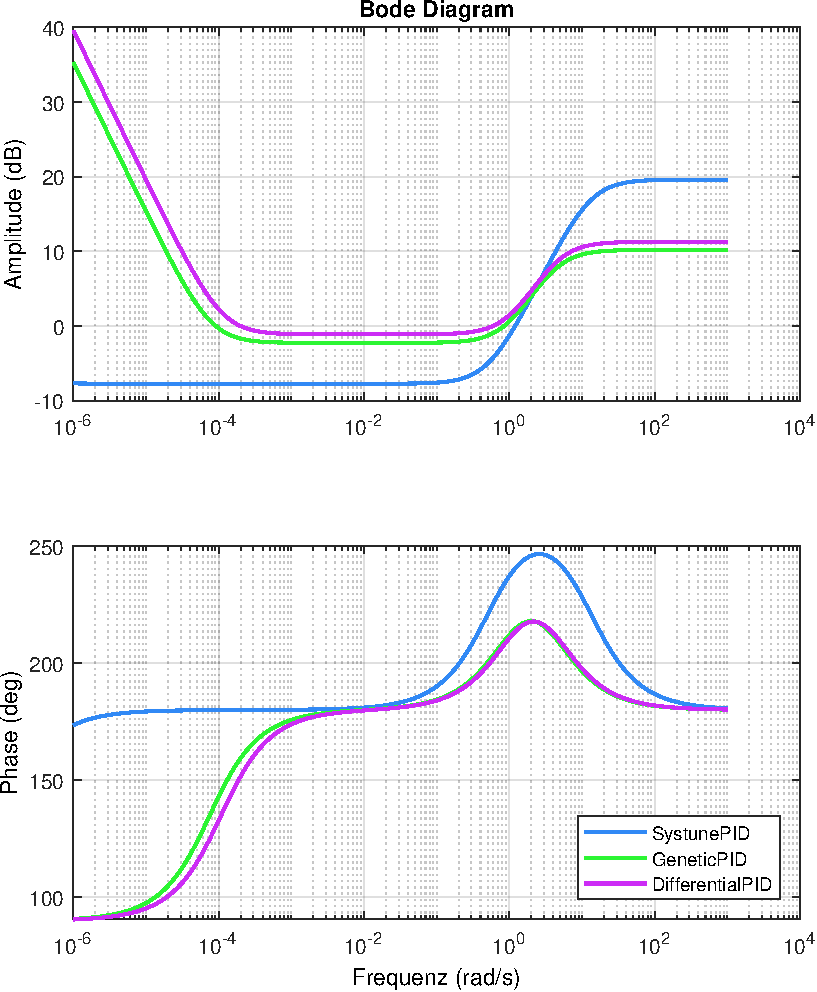
\includegraphics[width=\linewidth]{images/MotorMitSchwungmasse/CombinedMethodes_PIDBode.pdf}
        \caption{Bode-Diagramm der optimierten Regler}
        \label{fig:MotorMitSchwungmasseCombinedMethodes_PIDBode}
    \end{figure}
}

\newpage
\subsection{Frequenzanalyse der optimierten Systeme}
%\horizontalLine
\minipagedOrBelowEachOther
{
    \begin{figure}[H]
        \center
        %\vspace{-1.6cm}
        \includegraphics[width=\linewidth]{images/MotorMitSchwungmasse/CombinedMethodes_SystemBode.pdf}
        \caption{Bode-Diagramm der optimierten Vorwärts Pfade der einzelnen Systeme}
        \label{fig:MotorMitSchwungmasseCombinedMethodes_SystemBode}
    \end{figure}
    Das Bode-Diagramm in~\ref{fig:MotorMitSchwungmasseCombinedMethodes_SystemBode} und das
    Nyquist-Diagramm in~\ref{fig:MotorMitSchwungmasseCombinedMethodes_SystemLogScaleNyquist} zeigen,
    jeweils die Frequenzgänge der optimierten Vorwärts Pfade der drei Systeme:
    \begin{itemize}
        \item \textcolor{systuneColor}{$PID_{\mathbf{systune}} \cdot MotorSystem$}
        \item \textcolor{geneticColor}{$PID_{\mathbf{genetic}} \cdot MotorSystem$}
        \item \textcolor{differentialColor}{$PID_{\mathbf{differential}} \cdot MotorSystem$}
    \end{itemize}

    Im Nyquist-Diagramm fällt auf, dass der Regler von \textit{systune} seinem System deutlich mehr Phasenreserve bietet.
    Die Verstärkungsreserve ist bei den Reglern von GA und DE etwas höher als bei \textit{systune}, wobei aber 
    auch \textit{systune} mit 19.83dB eine sehr gute Verstärkungsreserve erreicht hat.  
}
{
    \begin{figure}[H]
        \center
        %\vspace{-1.6cm}
        \includegraphics[width=\linewidth]{images/MotorMitSchwungmasse/CombinedMethodes_SystemLogScaleNyquist.pdf}
        \vspace{-0.2cm}
        \caption{Logarithmisches Nyquist-Diagramm der optimierten Vorwärts Pfade der einzelnen Systeme \cite{matlabScriptNyquistLog}}
        \label{fig:MotorMitSchwungmasseCombinedMethodes_SystemLogScaleNyquist}
    \end{figure}

    \begin{table}[H]
        \center
        \begin{tabular}{@{}cr@{}}
                \toprule
                \textbf{Phasenreserve}              & \textbf{Wert} \\
                \midrule
                \textcolor{systuneColor}{\textit{Systune}}                          & 75.71 ° \\[0.5ex]
                \textcolor{geneticColor}{Genetisch}                        & 47.30 ° \\[0.5ex]
                \textcolor{differentialColor}{Differential Evolution}      & 46.30 ° \\[0.5ex]
                \hline
                \textbf{Verstärkungsreserve}              &  \\
                \hline
                \textcolor{systuneColor}{\textit{Systune}}                          & 19.83 dB \\[0.5ex]
                \textcolor{geneticColor}{Genetisch}                        & 21.92 dB \\[0.5ex]
                \textcolor{differentialColor}{Differential Evolution}      & 21.25 dB \\[0.5ex]
                \bottomrule
        \end{tabular}
        \caption{Reserven der optimierten Systeme}
        \label{tab:MotorMitSchwungmasseCombinedMethodes_AnalyzedData}
    \end{table}
}


\newpage
\subsection{Stabilitätsanalyse der optimierten Systeme}
\subsubsection{Sensitivität}
\begin{figure}[H]
    %\vspace{-1.6cm}
    \includegraphics[width=\linewidth]{images/MotorMitSchwungmasse/CombinedMethodes_Sensitivity.pdf}
    \caption{Sensitivität der optimierten Systeme}
    \label{fig:MotorMitSchwungmasseCombinedMethodes_Sensitivity}
\end{figure}
\minipagedOrBelowEachOther
{
    Das Sensitivitäts-Diagramm in \ref{fig:MotorMitSchwungmasseCombinedMethodes_Sensitivity} zeigt,
    für die mit \gls{GA} und \gls{DE} optimierten Systeme einen ähnlichen Verlauf.
    Beide haben eine stärkere Überhöhung im Vergleich zum mit \textit{systune} optimierten System.
    Insgesamt sind aber alle drei robuster gegenüber Totzeiten im Vergleich 
    zum System mit dem DC-Motor.
}
{

}

\horizontalLine
\begin{figure}[H]
    \subsubsection{Phasen- \& Verstärkungsreserve Diagramme der optimierten Systeme}
    \begin{minipage}[t]{0.32\textwidth}
        \begin{figure}[H]
            %\vspace{-1.6cm}
            \includegraphics[width=\linewidth]{images/MotorMitSchwungmasse/SystuneStabilityPhaseMarginsPlot.pdf}
            \caption{Phasen- \& Verstärkungsreserve des mit \textit{systune} optimierten Systems}
            \label{fig:MotorMitSchwungmasseSystuneStabilityPhaseMarginsPlot}
        \end{figure}
    \end{minipage}
    \hfill
    \begin{minipage}[t]{0.32\textwidth}
        \begin{figure}[H]
            %\vspace{-1.6cm}
            \includegraphics[width=\linewidth]{images/MotorMitSchwungmasse/GeneticStabilityPhaseMarginsPlot.pdf}
            \caption{Phasen- \& Verstärkungsreserve des mit Genetic optimierten Systems}
            \label{fig:MotorMitSchwungmasseGeneticStabilityPhaseMarginsPlot}
        \end{figure}
    \end{minipage}
    \hfill
    \begin{minipage}[t]{0.32\textwidth}
        \begin{figure}[H]
            %\vspace{-1.6cm}
            \includegraphics[width=\linewidth]{images/MotorMitSchwungmasse/DifferentialStabilityPhaseMarginsPlot.pdf}
            \caption{Phasen- \& Verstärkungsreserve des mit Differential Evolution optimierten Systems}
            \label{fig:MotorMitSchwungmasseDifferentialStabilityPhaseMarginsPlot}
        \end{figure}
    \end{minipage}


\minipagedOrBelowEachOther
{
    Die drei Diagramme in 
\ref{fig:MotorMitSchwungmasseSystuneStabilityPhaseMarginsPlot}, 
\ref{fig:MotorMitSchwungmasseGeneticStabilityPhaseMarginsPlot} und 
\ref{fig:MotorMitSchwungmasseDifferentialStabilityPhaseMarginsPlot}
    zeigen die detaillierten Stabilitätsreserven als Kombination von Verstärkung und 
    konstanter Phasenverschiebung.
    Wie diese Diagramme zu lesen sind, ist in folgendem Kapitel erklärt:\\
\fullref{sec:StabilitaetsPhaseMarginPlot}
}
{
    Die Stabile Region ist beim Regler von \textit{systune} am besten ausgeprägt. 
    Dieser bietet viel Spielraum für Phasenänderungen auch mit zusätzlicher Verstärkung.
    Die Regler von Genetic und Differential Evolution bieten eine ähnliche Stabile Region,
    welche nicht ganz so gross ist wie die von \textit{systune}.
}
\end{figure}


\newpage
\begin{figure}[H]
    \subsubsection{Totzeit- \& Verstärkungsreserve Diagramme der optimierten Systeme}
    \begin{minipage}[t]{0.32\textwidth}
        \begin{figure}[H]
            %\vspace{-1.6cm}
            \includegraphics[width=\linewidth]{images/MotorMitSchwungmasse/SystuneStabilityDelayMarginsPlot.pdf}
            \caption{Totzeit- \& Verstärkungsreserve des mit \textit{systune} optimierten Systems}
            \label{fig:MotorMitSchwungmasseSystuneStabilityDelayMarginsPlot}
        \end{figure}
    \end{minipage}
    \hfill
    \begin{minipage}[t]{0.32\textwidth}
        \begin{figure}[H]
            %\vspace{-1.6cm}
            \includegraphics[width=\linewidth]{images/MotorMitSchwungmasse/GeneticStabilityDelayMarginsPlot.pdf}
            \caption{Totzeit- \& Verstärkungsreserve des mit Genetic optimierten Systems}
            \label{fig:MotorMitSchwungmasseGeneticStabilityDelayMarginsPlot}
        \end{figure}
    \end{minipage}
    \hfill
    \begin{minipage}[t]{0.32\textwidth}
        \begin{figure}[H]
            %\vspace{-1.6cm}
            \includegraphics[width=\linewidth]{images/MotorMitSchwungmasse/DifferentialStabilityDelayMarginsPlot.pdf}
            \caption{Totzeit- \& Verstärkungsreserve des mit Differential Evolution optimierten Systems}
            \label{fig:MotorMitSchwungmasseDifferentialStabilityDelayMarginsPlot}
        \end{figure}
    \end{minipage}


\minipagedOrBelowEachOther
{
    Die drei Diagramme in 
\ref{fig:MotorMitSchwungmasseSystuneStabilityDelayMarginsPlot}, 
\ref{fig:MotorMitSchwungmasseGeneticStabilityDelayMarginsPlot} und 
\ref{fig:MotorMitSchwungmasseDifferentialStabilityDelayMarginsPlot}
    zeigen die detaillierten Stabilitätsreserven aus der Kombination von Verstärkung und 
    Totzeit.
    Wie diese Diagramme zu lesen sind, ist in folgendem Kapitel erklärt:\\
\fullref{sec:StabilitaetsDelayMarginPlot}
}
{
    Auch wenn die Verstärkungsreserve nicht beliebig gross ist, verhalten sich alle drei Systeme relativ robust
    gegenüber Kombinationen von Totzeit und Verstärkungsänderungen.
    Bei einer Verstärkung von 1, bleiben alle drei Systeme noch mit einer Totzeit von ca. 300ms stabil.
}
\end{figure}
\newpage



    \include{sections/80_Auswertung}

    
\section{Schlussteil}
\subsection{Objektives Fazit}
\subsubsection{\textit{Systune}}
\begin{itemize}
    \item[+] Mit \textit{systune} lassen sich Systeme schnell und mit wenig Code optimieren.
    \item[+] Die Tuning-Goals lassen sich einfach kombinieren.
    \item[+] \textit{Systune} bietet viele vordefinierte Tuning-Goals für unterschiedliche Kriterien an.  
    \item[+] \textit{Systune} ist in MATLAB integriert, wodurch der Grossteil der Komplexität nicht sichtbar ist.
    \item[+] \textit{Systune} übernimmt für die Optimierung die benötigten Simulationen im Zeit- und Frequenzbereich automatisch.
    \item[+] Erfordert keine Programmierkenntnisse um eine Optimierungsumgebung zu implementieren.
    \item[--] Die Parametrisierung der Tuning-Goals ist nicht immer einfach.
             Teilweise mangelt es an einer guten Dokumentation.
    \item[--] Die Tuning-Goals lassen sich nur in zwei Kategorien einteilen: hart und weich.
             Es gibt keine Möglichkeit die Priorität der Ziele zu gewichten.
    \item[--] Zu wenige vordefinierte Tuning-Goals für spezifische Kriterien.
    \item[--] Da nur lineare Systeme optimiert werden können, lassen sich keine Sättigungen oder Anti-Windup-Parameter optimieren.
             Anti-Windup-Parameter werden von MATLABs tunablePID ~\cite{matlabTunablePID} auch nicht angeboten.
    \item[--] Die Diagramme, welche die Optimierungsergebnisse der Tuning-Goals zeigen,
             sind nicht immer verständlich und teilweise nicht dokumentiert. 
             Höhere Fachkenntnisse sind deshalb notwendig um diese zu verstehen.
\end{itemize}

\minipagedOrBelowEachOther
{
    Die Optimierungsziele von MATLAB sind nicht ganz zufriedenstellend.
    Es gibt zwar vordefinierte Ziele, die für einige Kriterien verwendet werden können, 
    aber es bleibt noch viel Potenzial für weitere Ziele. Z.B Ziele für Rauschunterdrückung zwischen zwei Punkten im System fehlen.
    Die Parametrierung der Optimierungsziele ist teilweise etwas komplex, und die Beschreibung in der Dokumentation
    ist nicht immer sehr hilfreich.
}
{
    Um ein zufriedenstellendes Systemverhalten zu erreichen, 
    müssen die Optimierungsziele mehrfach angepasst, neue hinzugefügt oder entfernt werden.
    Teilweise führt das hinzufügen eines neuen Ziels dazu, dass ein schlechteres Ergebnis dadurch erzielt wird, 
    auch wenn die Ziele in einem realistischen Verhältnis zueinanderstehen.
}


\horizontalLine

\subsubsection{Differential Evolution Algorithmus}
\begin{itemize}
    \item[+] Auch durch das simple Optimierungsziel: Minimierung des aufsummierten, absoluten Fehlers,
             lässt sich schon ein sehr guter Regler finden.
    \item[+] Sehr flexibel, es können beliebige Systeme optimiert werden, auch nichtlineare (nur zeitinvariante).
    \item[+] Die Optimierungsziele sind frei definierbar.
    \item[+] Der Algorithmus ist relativ einfach zu verstehen und zu implementieren.
    \item[+] Konvergiert sehr schnell.
    \item[--] Findet nicht immer eine gute Lösung.
    \item[--] Für die Optimierung muss mehr Code geschrieben werden oder eine Toolbox gefunden werden, die einem viel Arbeit abnimmt.
    \item[--] Die Definition der \gls{Fitnessfunktion} ist nicht immer einfach, 
             da alle Optimierungsziele in einer einzigen Formel sind.
    \item[--] Die Gewichtung der unterschiedlichen Kriterien in der Fitnessfunktion
             ist nicht immer einfach zu bestimmen und erfordert mehrere Anläufe.
    \item[--] Erfordert höhere Programmierkenntnisse um die Optimierungsumgebung zu implementieren.
\end{itemize}

\minipagedOrBelowEachOther
{
    \gls{DE} hat sehr ähnliche Vor- und Nachteile wie der \gls{GA}.
    Der Algorithmus konvergiert jedoch schneller und hat einen schöneren Konvergenzverlauf.
    DE garantiert, dass die \gls{Population} nicht schlechter wird mit jeder Generation,
    unterliegt aber auch oft dem Problem zu früh in einem lokalen Minimum stecken zu bleiben.
}
{
    DE ist in der Lage aus lokalen Minima herauszukommen, wenn die Streuung der Population nicht zu klein wird.
    Für den DE müssen die Optimierungsumgebung und die Datenerhebung selbst implementiert werden, wie beim GA.
}


\newpage
\subsubsection{Genetischer Algorithmus}
\begin{itemize}
    \item[+] Auch durch das simple Optimierungsziel: Minimierung des aufsummierten, absoluten Fehlers,
             lässt sich schon ein sehr guter Regler finden.
    \item[+] Sehr flexibel, es können beliebige Systeme optimiert werden, auch nichtlineare (nur zeitinvariante).
    \item[+] Die Optimierungsziele sind frei definierbar. 
    \item[+] Der Algorithmus ist ziemlich einfach zu verstehen und zu implementieren. 
    \item[--] Findet nicht immer eine gute Lösung.
    \item[--] Für die Optimierung muss mehr Code geschrieben werden oder eine Toolbox gefunden werden, die einem viel neue Codierung abnimmt.
    \item[--] Die Definition der \gls{Fitnessfunktion} ist nicht immer einfach, 
             da alle Optimierungsziele in einer einzigen Formel sind.
    \item[--] Die Gewichtung der unterschiedlichen Kriterien in der Fitnessfunktion.
             ist nicht immer einfach zu bestimmen und erfordert mehrere Anläufe.
    \item[--] Erfordert höhere Programmierkenntnisse um die Optimierungsumgebung zu implementieren.
\end{itemize}

\minipagedOrBelowEachOther
{
    Anders als mit \textit{systune} muss die Optimierungsumgebung selbst implementiert werden.
    In dieser Arbeit wurde auch der GA selbst implementiert, 
    obwohl MATLAB eine fertige Implementierung anbietet \cite{matlabGeneticAlgorithm}.
    Die Optimierungsziele müssen programmiert werden, 
    was für sehr spezifische Anforderungen aufwendig sein kann.

    Eine Schwierigkeit bei der Verwendung des GA liegt einerseits in der Definition der Fitnessfunktion,
    welche bei \gls{Minimierungsproblem}en eine spezifische Umwandlung erfordert, nur ein Vorzeichenwechsel funktioniert nicht.
    Andererseits müssen die Optimierungsziele als Formel ausgedrückt werden die in einem einzigen Wert resultieren.
    Die Problematik besteht darin, die richtigen Formeln für die unterschiedlichen Kriterien zu erstellen und 
    diese auch noch in ein gutes Verhältnis zueinander zu setzen. (Gewichtung der Bewertungskriterien)
    Deshalb benötigt auch diese Methode mehrere Anläufe beim Erstellen der Fitnessfunktion 
    bis ein zufriedenstellendes Systemverhalten erzielt wird.\\


    Der GA hat den Nachteil, dass sich die zu optimierenden Parameter nur schwer einschränken lassen.
    In spezifischen Fällen ist im Vorhinein bekannt, dass gewisse Bereiche von Parametern nicht möglich sind.
    Diese Bereiche lassen sich im GA nur schwer ausschliessen, da der Algorithmus zufällig neue Individuen generiert.
    Eine Möglichkeit wäre, die Fitness dieser Individuen sehr schlecht zu bewerten.\\


    Ein weiterer Nachteil des GA besteht darin, dass der Algorithmus am besten auf gleich normierte Parameter anwendbar ist.
    Befinden sich bestimmte Parameter in einem viel grösseren Werte-Bereich als andere, 
    kann es sein dass die Mutations-Stärke für einige Parameter zu klein ist und für andere zu gross.
    Bei gleich normierten Parametern entfällt dieses Problem.
    Eine Lösung hierfür wäre, entweder die Parameter normiert dem Algorithmus zu übergeben,
    oder den Algorithmus so anzupassen, dass die Mutations-Stärke für jeden Parameter individuell skaliert ist.
    Es gibt verschiedenste Strategien für die individuelle Mutation eines Gens. (Stichwort: \textit{self-adaptive mutation})

}
{
    Mit stetigem verkleinern der Mutations-Stärke kann die Geschwindigkeit der \gls{Konvergenz} erhöht werden, 
    wodurch der GA vergleichbar schnell wie DE konvergiert.
    Sein stochastisches Verhalten hilft dabei, nicht zu schnell in lokalen Minima stecken zu bleiben.\\


    Damit die Optimierung überhaupt durchgeführt werden kann, müssen für die Fitnessfunktion die benötigten Daten 
    ermittelt werden, diese können einerseits aus einer Simulation des Systems im Zeitbereich stammen,
    andererseits können auch frequenzabhängige Messungen durchgeführt werden.
    Diese Datenerhebung muss allenfalls selbst implementiert werden und kann je nach Anwendungsfall und Anforderung an das 
    Reglerverhalten beliebig komplex werden.
    Dafür sind weitere Programmierkenntnisse notwendig im Bereich der numerischen Simulation von Systemen und 
    der Frequenzanalyse notwendig.
    Natürlich lässt sich die Optimierung mit MATLAB und Simulink durchführen wodurch die Probleme der manuellen Implementierung 
    einer Simulation und Frequenzanalyse entfallen, aber auch dann kann noch viel Aufwand bei der Implementierung der
    Optimierungsumgebung entstehen.
    Das sind Aspekte welche nichts mit dem \gls{GA} an sich zu tun haben, aber trotzdem notwendig sind um den Algorithmus
    anwenden zu können. 
}



\horizontalLine
\subsubsection{Welche ist die beste Methode?}
\minipagedOrBelowEachOther
{
    Welche Methode besser geeignet ist, 
    lässt sich nicht allgemein sagen und hängt stark vom jeweiligen Anwendungsfall ab.
    Die Tests der drei Methoden an nur zwei Prozessen sind nicht ausreichend um eine allgemeingültige Aussage treffen zu können.
    Für eine fundierte Aussage wären deutlich mehr Tests an sehr unterschiedlichen Prozessen notwendig.\\


    Mit \textit{systune} lässt sich schneller ein Regler entwerfen und testen als mit den anderen beiden Methoden.
    Allerdings wird es schwierig mit \textit{systune} den Regler auf allfällig folgende weitere Anforderungen zu verfeinern,
    da sich solche Anforderungen nicht, oder nur ungenügend, in den vorhandenen Tuning-Goals abbilden lassen.
}
{
    Für GA und DE ist es einfacher weitere Anforderungen in der Fitnessfunktion zu berücksichtigen.
    Ein Kriterium kann frei definiert und gewichtet werden und bietet somit von einfach bis beliebig komplex viele Möglichkeiten.
    Die Flexibilität und die Möglichkeit beliebige nichtlineare Systeme zu optimieren, 
    bietet ausserdem den grossen Vorteil, dass sich der Regler besser auf reale Bedingungen abstimmen lässt.
}


\newpage
\subsubsection{Iteratives Tuning der Methoden}
\label{sec:objektivesFazitIterativesTuning}
\minipagedOrBelowEachOther
{
    Alle drei Methoden erfordern ein iteratives Vorgehen um ein gutes Ergebnis zu erhalten.\\


    \paragraph*{\textit{Systune}}
    Bei \textit{systune} müssen die Tuning-Goals angepasst werden, bis ein zufriedenstellendes Ergebnis erzielt wird.
    Verschiedene Kombinationen von Zielen und deren Parameter müssen ausprobiert werden,
    denn nicht immer führt das Hinzufügen eines neuen Ziels zu einem besseren Ergebnis.\\


    %\paragraph[Genetischer Algorithmus und Differential Evolution]{
    %    \parbox[t]{\dimexpr\textwidth\relax}{
    %        Genetischer Algorithmus und\\Differential Evolution}
    %    }
    \paragraph*{Genetischer Algorithmus und\\Differential Evolution}

    Bei \gls{GA} und \gls{DE} muss die Fitnessfunktion angepasst werden, bis ein zufriedenstellendes Ergebnis erzielt wird.
    Ausserdem müssen für eine Simulation im Zeitbereich die Stimulationssignale so gewählt werden,
    dass die gewünschten Kriterien auch tatsächlich in die Fitness der Population mit einfliessen.
    Die Hyperparameter des Algorithmus müssen teilweise angepasst werden.
    In der Regel genügen die Standardeinstellungen für einen Grossteil der Anwendungen aus aber
    in spezifischen Fällen kann es notwendig sein, diese anzupassen um bessere Ergebnisse zu erzielen.
}
{
    Der implementiere PID-Regler hat viele Einstellmöglichkeiten um unterschiedliche Kombinationen zu testen.
    Schlussendlich wurden jedoch nur die einfachsten Einstellungen verwendet.
    \textit{Systune} kann keinen Anti-Windup optimieren, weshalb sich die verwendete Anti-Windup-Strategie auf 
    \textit{Clamping}~\ref{par:Clamping} beschränkt.
    Diese Methode benötigt keinen zusätzlichen Parameter und ist im Simulink PID-Regler-Block bereits integriert.\\
    

    Bei \gls{GA} und \gls{DE} wurde der PID-Regler direkt mit dieser Anti-Windup-Strategie optimiert.
    Auch die Anti-Windup-Strategie \textit{Back-Calculation}~\ref{par:Back-Calculation}, 
    bei der ein zusätzlicher Parameter optimiert werden muss, wurde ausprobiert. Dies hat auch zu guten Ergebnissen geführt,
    jedoch wurde schlussendlich auf die einfachere \textit{Clamping} Methode zurückgegriffen, 
    um den Vergleich mit \textit{systune} fairer zu gestalten.\\


    Auch die Filterkonstante für den D-Anteil ist optional und lässt sich im Simulink PID-Regler-Block aktivieren oder deaktivieren.
    Das gleiche gilt für die Implementierung in der C++ Simulation.
    Da \textit{systune} aber die Filterkonstante immer mitoptimiert, wurde dies auch bei \gls{GA} und \gls{DE} so gehandhabt.
}

\paragraph{Bestimmung der Hyperparameter bei \gls{GA} und \gls{DE}}
\minipagedOrBelowEachOther
{
    Für die Bestimmung der Hyperparameter wurde viel ausprobiert.
    Gewisse Parameter haben grösseren Einfluss auf den Optimierungsprozess und andere weniger.
    Das finden der optimalen Hyperparameter ist in sich selbst ein Optimierungsproblem.
}
{}
\minipagedOrBelowEachOther
{
    \subparagraph{Populationsgrösse}
    \noindent
    \\
    Die gewählte Populationsgrösse ist abhängig von der Komplexität des Problems,
    also wie viele Parameter optimiert werden müssen.
    Je komplexer das Problem, desto grösser sollte die Population gewählt werden,
    um den Suchraum besser abdecken zu können.
    Zu gross sollte die Population aber auch nicht gewählt werden,
    da dies die Rechenzeit unnötig in die Höhe treibt und ab einer bestimmten Grösse kaum noch Vorteile bringt.\\


    \subparagraph{Anzahl Generationen}
    \noindent
    \\
    Dieser Parameter definiert, wie oft die Population aktualisiert wird.
    Je komplexer das Problem, desto mehr Generationen werden benötigt.
    Dieser Parameter wird als Abbruchbedingung der Optimierung verwendet und kann je nach Implementierung auch 
    weggelassen werden, um stattdessen ein anderes Abbruchkriterium zu verwenden, 
    wie z.B. ein Unterschreiten des Fehlers unter einen bestimmten Wert.\\
}
{
    \subparagraph{Mutations-Stärke}
    \noindent
    \\
    Die Mutations-Stärke definiert, wie stark eine Mutation ausfällt.
    Je grösser die Mutations-Stärke, desto grösser werden die Veränderungen an den zu mutierenden Genen.
    Eine grosse Mutations-Stärke kann dabei helfen, aus lokalen Minima herauszukommen,
    jedoch kann eine zu grosse Mutations-Stärke auch dazu führen, dass die Optimierung nicht konvergiert.
    Im Fall vom \gls{GA} wurde die Mutations-Stärke im Verlauf der Optimierung verkleinert um die Vorteile von grossen und kleinen
    Mutationen zu kombinieren.
    Für \gls{DE} muss die Mutations-Stärke nicht angepasst werden, da diese automatisch durch die abnehmende Distanz zweier Individuen im Verlauf
    der Optimierung abnimmt.\\


    \subparagraph{Konstante Systemparameter}
    \noindent
    \\
    Systemparameter der Regelstrecke welche nicht optimiert wurden, 
    sind von Hand festgelegt worden. Die Sättigung des I-Anteils des PID-Reglers ist ein Beispiel dafür.
    In beiden getesteten Systemen wird ein gutes Ergebnis erzielt, sowohl mit einer Sättigung als auch ohne.
    Deshalb ist eine genaue Bestimmung dieser Parameter nicht kritisch.\\  
}
\minipagedOrBelowEachOther
{
    \subparagraph{Mutations-Wahrscheinlichkeit (nur \gls{GA})}
    \noindent
    \\
    Die Mutations-Wahrscheinlichkeit definiert, die Wahrscheinlichkeit, dass ein Genom eines Individuums mutiert wird.
    Ein Genom ist eine einzelne Variable des Individuums, also z.B. ein Reglerparameter.
    Je höher die Mutations-Wahrscheinlichkeit, desto grösser die Diversität in der Population.
    Eine zu hohe Mutations-Wahrscheinlichkeit kann jedoch dazu führen, dass die Optimierung nicht konvergiert.
    Dies kann mit einer radioaktiven Umgebung verglichen werden, in der sich die Individuen ständig verändern und 
    somit langfristig keine auf das Problem abgestimmte Population entstehen kann.
    Je mehr Parameter ein Individuum hat, desto kleiner sollte die Mutations-Wahrscheinlichkeit gewählt werden,
    um nicht zu viele Mutationen pro Generation zu erzeugen.
    Ein zu kleiner Wert schadet nur der Zeit, die für die Konvergenz benötigt wird. 
    Ein zu grosser Wert kann jedoch verhindern, dass eine gute Lösung gefunden wird.\\

}
{
    \subparagraph{Startwerte gesuchten Parameter}
    \noindent
    \\
    Die Startwerte der zu optimierenden Parameter können einen grossen Einfluss auf die Konvergenzgeschwindigkeit haben, 
    bzw. generell darauf, ob überhaupt eine gute Lösung gefunden wird.\\


    In dieser Arbeit wurde eine zufällige Initialisierung der Parameter in der Umgebung um den Nullpunkt verwendet.
    Die Wahl der Grösse der Startumgebung ist abhängig von der ungefähren Grössenordnung der zu optimierenden Parameter.
    Es lohnt sich, mit der Grösse des Startbereichs zu experimentieren.\\


    Bei bestimmten Problem stehen eventuell schon gute Startwerte zur Verfügung oder es gibt bekannte Bereiche,
    in denen sich gute Lösungen befinden.
    In solchen Fällen sollten diese Informationen genutzt werden, um die Startwerte entsprechend zu wählen.\\   
}

\newpage


\subsection{Persönliches Fazit}
\minipagedOrBelowEachOther
{
    Eigentlich war geplant den \gls{GA} und den \gls{DE} Algorithmus 
    in Kombination mit der Ziegler-Nichols Methode zu verwenden. 
    Die gewählten Prozesse lassen dies jedoch nicht zu, da sie entweder instabil sind
    oder nur sehr kleine Zeitkonstanten haben.\\
    

    Die Optimierung, ohne die durch Ziegler-Nichols bestimmten Startwerte,
    hat jedoch an beiden Prozessen gut funktioniert und deshalb bietet Ziegler-Nichols
    keinen Mehrwert für diese Optimierungsmethoden.
    Ausserdem wäre Ziegler-Nichols nur für PID-Regler anwendbar,
    während die Optimierungsmethoden beliebige Reglerstrukturen optimieren können.\\

    
    Es konnten leider nicht alle geplanten Aufgaben umgesetzt werden.
    Eine Demo Applikation zur Visualisierung der Optimierungsprozesse
    ist nicht genug überarbeitet um sie mit dieser Arbeit abgeben zu können.
    Mein Ziel ist es jedoch, auch nach der Abgabe der Arbeit die Applikation noch aufzuräumen 
    und auf GitHub zu veröffentlichen \cite{baRepository}.
}
{
    \subsubsection{\textit{Systune}}
    Die Optimierung mit \textit{systune} hat aus meiner Sicht nicht so gut funktioniert wie ich 
    das erhofft hatte.
    Ich glaube, dass mit tieferem Wissen über \textit{systune} und die Tuning-Goals, 
    ein besseres Ergebnis erzielt werden könnte.
    Eine bessere Dokumentation von Seite Mathworks wäre sehr hilfreich gewesen.\\
   

    Teilweise habe ich mittels Testen von neuen Tuning-Goals festgestellt, dass die Optimierung völlig versagt.
    Ohne Rückmeldung dazu, was genau an dem neu hinzugefügten Tuning-Goal falsch ist, ist es schwierig
    zu verstehen, warum die Optimierung damit nicht funktioniert. Manchmal hatten auch bestimmte Tuning-Goals 
    Einflüsse auf Dynamiken des Systems, welche ich nicht erwartet hätte oder nicht in diesem Ausmass.
    Viele Tuning-Goals musste ich deshalb wieder aus der Optimierung entfernen, weil ich es nicht geschafft habe diese 
    korrekt zu konfigurieren.
}
%\horizontalLine
\minipagedOrBelowEachOther
{
    \subsubsection{Genetischer Algorithmus}
    Der genetische Algorithmus ist nicht allzu kompliziert zu verstehen und lässt sich relativ einfach implementieren.
    Es gibt sogar eine fertige Implementierung in MATLAB ~\cite{matlabGeneticAlgorithm}, aber diese habe ich nicht angeschaut.
    Die eigene Implementierung hat es mir ermöglicht, einen kompletten Einblick in den Optimierungsprozess zu bekommen.
}
{
    \subsubsection{Differential Evolution Algorithmus}
    Der Differential Evolution Algorithmus ist ein wenig schwieriger zu verstehen als der genetische Algorithmus,
    aber die Implementierung ist auch hier relativ einfach. 
    Im Gegensatz zum genetischen Algorithmus kannte ich \gls{DE} vor der Arbeit noch nicht aber für zukünftige Projekte, 
    welche einen Optimierungsalgorithmus benötigen, werde ich \gls{DE} definitiv ausprobieren.
}


\horizontalLine
\subsubsection{Welches ist die beste Methode?}
\minipagedOrBelowEachOther
{
    Ich persönlich bevorzuge den GA und den
    DE-Algorithmus, da sie bessere Möglichkeiten für
    spezifische Optimierungsziele bieten.\\


    Ich glaube durchaus, dass \textit{systune} in der Lage wäre mit den geeigneten Optimierungszielen 
    ein besseres Ergebnis zu liefern als das was ich es in der Arbeit erzielt habe, 
    aber dennoch sehe ich den grösseren Vorteil darin ein nichtlineares System optimieren zu können. \\

    Sättigungen sind da ein gutes Beispiel, welche bei realen Systemen immer vorhanden sind
    und das Systemverhalten stark beeinflussen können.
    Beispielsweise lassen sich stabile Regler für Systeme mit Sättigung umsetzen welche im linearisierten Fall ohne Sättigung 
    instabil wären. Wird der Regler jedoch auf das linearisierte System optimiert, so ist das System zwar stabil, 
    verschenkt aber im realen Prozess mögliche Leistungspotentiale.
}
{
    Sättigungen im System in Kombination mit Integratoren im Regler führen zum Windup-Problem, welches leider mit \textit{systune} nicht
    mitberücksichtigt werden kann.
    Mit dem genetischen- oder dem Differential Evolution Algorithmus können unterschiedliche
    Anti-Windup-Methoden sowie deren Parameter in die Optimierung einbezogen werden,
    was auch dafür sorgt, dass die Nebeneffekte der Anti-Windup-Methoden berücksichtigt werden.
}


\newpage
\subsubsection{Zu spät erkannte Fehler}
\minipagedOrBelowEachOther
{
    \paragraph*{Falsche Normierung der\\Fehler-Minimierungs-Funktion}

    Während der Überarbeitung der Arbeit ist mir aufgefallen, 
    dass die ~\fullref{form:SimpleMotorGeneticAlgorithmErrorMinimizationFunction}
    fälschlicherweise wie folgt definiert wurde:

    \begin{equation*}
        %\label{form:SimpleMotorGeneticAlgorithmErrorMinimizationFunction}
		\mathFunction{g}{I_{\mathbf{i}}} = 
		\frac{1}{t_\mathbf{end}-t_\mathbf{start}}\sum_{k=0}^{K-1}(
				\sum_{o=0}^{O-1}(
					a_\mathbf{o} \cdot \mathFunction{g_\mathbf{o}}{k}
				)
			)
	\end{equation*}

    Der Fehler liegt in dem Skalierungsfaktor $\frac{1}{t_\mathbf{end}-t_\mathbf{start}}$,
    dieser müsste eigentlich $\frac{1}{K}$ sein, also die Anzahl der Zeitschritte.
    Da für jeden Simulationsschritt die jeweiligen Teilsummen addiert werden,
    muss der \gls{Fehler} durch die Anzahl der Zeitschritte normiert werden und nicht durch die Simulationszeit.\\


    Das gleiche Problem tritt beim zweiten getesteten Prozess auf.\\
    ~\ref{form:MotorMitSchwungmasseGeneticAlgorithmErrorMinimizationFunction}:

    \begin{equation*}
		%\label{form:MotorMitSchwungmasseGeneticAlgorithmErrorMinimizationFunction}
		\mathFunction{g}{I_{\mathbf{i}}} = 
		\frac{1}{t_\mathbf{end}-t_\mathbf{start}}\sum_{k=0}^{K-1}(
				\sum_{o=0}^{O-3}(
					a_\mathbf{o} \cdot \mathFunction{g_\mathbf{o}}{k}
				)
			) + a_\mathbf{3} \cdot \mathFunction{g_\mathbf{3}}{I_{\mathbf{i}}}
			  + a_\mathbf{4} \cdot \mathFunction{g_\mathbf{4}}{I_{\mathbf{i}}}
	\end{equation*}

    Beide Fehler sind in der Dokumentation korrigiert und haben auch keinen Einfluss auf die Resultate der Arbeit.
    Die einzige Inkonsistenz die dadurch entsteht, ist dass die gemessenen Lernkurven falsch skaliert sind.\\

    
    Ich empfehle eine Normierung der Bewertungsfunktion, aber es ist theoretisch nicht zwingend notwendig,
    solange die Anzahl der Zeitschritte in der Simulation pro Trainings-Iteration für jedes Individuum gleich bleibt.
    Notwendig ist eine Normierung dann, wenn die Individuen mit unterschiedlichen Simulationszeiten oder Abtastzeiten bewertet werden,
    da in diesem Fall z.B. für Individuum A, 10-mal die Regelabweichung integriert wird und für Individuum B nur 5 mal.
    Das würde dafür sorgen, dass Individuum A einen grösseren Fehlerwert erhält als Individuum B und somit 
    beim Selektionsprozess benachteiligt wird.
}
{
    \paragraph*{Dynamisches anpassen der Bewertungsfunktion}
    %\phantomsection
    \label{par:objektivesFazitDynamischeAnpassungBewertungsfunktion}
    Im Beispiel des Motors mit Schwungmasse wird die Teilbewertung $\mathFunction{g_\mathbf{4}}{I_{\mathbf{i}}}$ erst ab Epoche
    100 in die Gesamtbewertung einbezogen. Dies hat zu starke Schwankungen in der Lernkurve geführt, wie in
    \fullref{fig:MotorMitSchwungmasseGenetic_SimulationLearningHistory_1} zu sehen ist.


    Im Test mit dem \gls{DE} ist jedoch kein solcher Sprung in der Lernkurve zu erkennen.
    Der Grund dafür liegt in der Natur des \gls{DE} Algorithmus.
    Der \gls{DE} bevorzugt immer das bessere Individuum in der Population, gegenüber dem jeweils neu getesteten Individuum.
    Sobald die Teilbewertung $\mathFunction{g_\mathbf{4}}{I_{\mathbf{i}}}$ in die Gesamtbewertung einbezogen wird,
    wird der Durchschnittsfehler der Population sofort schlechter.
    Der \gls{DE} sorgt jedoch dafür, dass deshalb alle neuen Individuen verworfen werden weil sie 
    schlechter sind als die bisherigen Individuen.
    Dadurch sieht es so aus als würde \gls{DE} die hinzugefügte Teilbewertung sehr gut verkraften.
    Dies ist jedoch nicht der Fall.\\


    Im Gegensatz zum \gls{GA} ist \gls{DE} abhängig von den \gls{Fehler}werten der alten Population.
    Deshalb darf eine solche Änderung der Bewertungsfunktion nicht vorgenommen werden, ausser es wird garantiert,
    dass durch die Anpassung der Bewertungsfunktion, der durchschnittliche Fehlerwert der Population verbessert wird.\\

    
    Der \gls{GA} hingegen ist nicht von diesem Problem betroffen, da jede Generation komplett individuell betrachtet wird und
    grosse Sprünge in den durchschnittlichen Fehler der Population keine Auswirkungen auf die Selektion der Individuen haben.\\

    Dieses Problem ändert jedoch nicht grossartig das erzielte Resultat,
    da der \gls{DE} zum Zeitpunkt als die Teilbewertung hinzugefügt wird, sowieso schon so
    gut ist, dass die Fehlerwerte die durch die Teilbewertung $\mathFunction{g_\mathbf{4}}{I_{\mathbf{i}}}$
    hinzugefügt werden, im Vergleich zu den anderen Teilbewertungen sehr klein sind.
}

%\horizontalLine
%\subsubsection{Welches ist die beste Methode?}
%\minipagedOrBelowEachOther
%{
%
%}
%{
%
%}

\newpage
%\horizontalLine
\subsubsection{Herausforderungen \& Learnings}

\minipagedOrBelowEachOther{
    \paragraph*{Die erste Arbeit mit LaTeX}
    Dies ist meine erste Arbeit, die ich mit LaTeX verfasst habe.
    Schon seit längerer Zeit hatte ich mir vorgenommen, LaTeX zu erlernen, 
    jedoch war die Hemmschwelle dafür stets sehr hoch.
    Obwohl mir die Wahl des Werkzeugs freigestanden hätte, habe ich mich bewusst dafür entschieden, 
    diese Arbeit in LaTeX zu schreiben.
    Es bot sich dadurch eine gute Gelegenheit, mich intensiv mit LaTeX auseinanderzusetzen.

    Die Arbeit mit LaTeX hat mich teilweise viel Geduld gekostet, 
    dennoch bin ich froh, diesen Schritt gegangen zu sein.
    Besonders störend empfand ich die Fehlersuche: Tritt ein Fehler auf, 
    wird häufig nicht eindeutig angezeigt, wo dieser tatsächlich liegt.
    Stattdessen meldet der Compiler Probleme an anderen Stellen, was die Fehlersuche erschwert.

    Aus programmiertechnischer Sicht sehe ich ebenfalls Verbesserungspotenzial.
    Meiner Meinung nach könnte LaTeX deutlich mächtiger sein, 
    wenn es syntaktisch und strukturell besser aufgebaut wäre.
}
{
    \paragraph*{MATLAB Programmierung für die Regleroptimierung und Erstellung von Grafiken}
    Vor Beginn dieser Arbeit hatte ich nur wenig Erfahrung mit der Programmierung in MATLAB.
    Für die automatisierte Erstellung der Grafiken erwies sich MATLAB jedoch als sehr hilfreich.
    Um den Aufwand zu reduzieren, habe ich ein Skript entwickelt, 
    das per Knopfdruck nahezu alle Grafiken der Arbeit erzeugt und automatisch im vorgesehenen Verzeichnis speichert.
}
\minipagedOrBelowEachOther{
    \paragraph*{Implementierung der Systeme und\\Optimierungsalgorithmen in C++}
    Für die Implementierung von GA und DE habe ich mich für C++ entschieden, 
    da ich diese Sprache gut beherrsche und damit im Vergleich zu
    anderen Sprachen schneller Ergebnisse erzielen kann. 
    Als Grundlage für die C++-Applikation diente meine eigene, 
    einfache Game-Engine \cite{cppLibraryQSFMLEditorWidget}, 
    die es mir ermöglichte, mich rasch auf die wesentlichen Aspekte der Implementierung zu konzentrieren.
    Zudem liessen sich grafische Visualisierungen mit dieser Basis unkompliziert realisieren.
}
{
    \paragraph*{Auffrischung der Z-Transformation}
    Für die diskrete Simulation der Systeme musste ich mich zum ersten Mal 
    seit langer Zeit wieder mit der Z-Transformation befassen. 
    Das Erreichen eines lauffähigen Ergebnisses erwies sich dabei als 
    sehr motivierend und steigerte die Freude an der Thematik.
}
\minipagedOrBelowEachOther
{
    \paragraph*{Implementierung von unterschiedlichen\\diskreten Integrationsverfahren}
    Für die diskrete Simulation der Systeme habe ich mich entschieden, verschiedene Integrationsverfahren zu implementieren.
    Dies ermöglicht es, problemlos zwischen den unterschiedlichen Verfahren zu wechseln,
    um die Genauigkeit der Simulation gezielt zu optimieren.
}
{
    \paragraph*{Modellbildung des Prozesses:\\Motor mit Schwungmasse}
    Bei der Modellbildung des Prozesses konnte nicht auf die dokumentierten Modellbeschreibungen zurückgegriffen werden, 
    da diese ein anderes Systemverhalten als der reale Prozess abbilden.
    Daher wurde das Modell des Prozesses mithilfe einer Systemidentifikation erstellt. \ref{sec:MotorMitSchwungmasseModellidentifikation}
    Mir kam die Idee, den GA in diesem Zusammenhang zu nutzen, anstatt mich lange mit manueller Parametrierung aufzuhalten. 
    Um den GA für die Modellidentifikation zu nutzen, musste lediglich das strukturelle Modellgerüst definiert werden,
    während die Parameteroptimierung automatisch durch den Algorithmus erfolgte.
}
\minipagedOrBelowEachOther{
    \paragraph*{Alternative Darstellung des Nyquist-Diagramms}
    Um das Nyquist-Diagramm darzustellen, habe ich mich gegen die klassische Darstellung von
    MATLAB entschieden, da ich sie nicht besonders übersichtlich finde.
    Stattdessen habe ich das Nyquist-Diagramm mit eines externen MATLAB-Skript \cite{matlabScriptNyquistLog} 
    in einer logarithmischen Darstellung geplottet.
    Um mehrere Systeme innerhalb desselben Diagramms darstellen zu können, 
    waren einige Anpassungen am Skript erforderlich.
    Die resultierende Darstellung bietet meiner Ansicht nach eine übersichtlichere und verständlichere Visualisierung.
    Das Skript ist nicht perfekt aber für die Zwecke dieser Arbeit ausreichend.
}
{
    \paragraph*{Alternative Darstellung der Stabilitätsgrenzen}
    Bei der Recherche zur Interpretation des Resultatdiagramms vom Optimierungskriterium \textbf{TuningGoal.Margins} \cite{matlabTuningGoals_Margins},
    bin ich auf ein Video von Brian Douglas gestossen \cite{matlabScriptStabilityRegionPlot}.
    In diesem Video wird eine alternative Darstellung der Stabilitätsgrenzen eines Systems erläutert.
    Die dort gezeigte Visualisierung wurde jedoch nicht vollständig übernommen, 
    da sie einen Teil des möglichen Stabilitätsbereichs ausblendet.
    Stattdessen konzentrierte ich mich auf den Teil des Videos, in dem er zeigte, 
    wie man für jeden Punkt berechnet, ob das System stabil ist oder nicht. 
    Auf dieser Grundlage entstand der\\
    \fullref{sec:StabilitaetsPhaseMarginPlot}.

    Nach einer Diskussion mit \Betreuer~wurde deutlich, 
    dass diese Darstellung in der praktischen Anwendung nur eingeschränkt hilfreich ist.
    Sie setzt voraus, dass die Phasenverschiebung über den gesamten Frequenzbereich konstant ist.
    In realen Systemen entstehen Phasenverschiebungen jedoch unter anderem auch durch Totzeiten, 
    welche dann in frequenzabhängigen Phasenverschiebungen enden.
    Aus diesem Grund wurde ein weiteres Diagramm entwickelt, 
    das den Einfluss von Verstärkung und Totzeit auf die Stabilität des Systems veranschaulicht.\\
    \fullref{sec:StabilitaetsDelayMarginPlot}
}
\newpage

\minipagedOrBelowEachOther
{
    \paragraph*{Stabilitätsanalysen}
    Im Verlauf der Arbeit sind immer wieder neue Möglichkeiten zur Stabilitätsanalyse aufgetaucht.\\
   ~\fullref{sec:StabilitaetsPhaseMarginPlot},\\
   ~\fullref{sec:StabilitaetsDelayMarginPlot}\\
    und das Sensitivitäts-Diagramm wurden zu einem Zeitpunkt hinzugefügt,
    an dem ich schon alle Tests und Messungen abgeschlossen hatte.
    Die zusätzlichen Stabilitätsanalysen haben aber gezeigt, dass z.B. die optimierten Systeme für den DC-Motor
    zwar gute Verstärkungs- und Phasenreserven haben, aber sehr empfindlich auf Totzeiten reagieren. 
    Für ein robusteres Systemverhalten wäre es notwendig gewesen, 
    die Tuning-Goals und die Fitnessfunktionen dementsprechend anzupassen.
}
{
    \paragraph*{Dynamisches anpassen der\\Bewertungsfunktion für \gls{DE}}
    Wie bereits auf Seite \pageref{par:objektivesFazitDynamischeAnpassungBewertungsfunktion}: '\textbf{Dynamisches anpassen der Bewertungsfunktion}' beschrieben,
    ist es heikel, die Bewertungsfunktion für \gls{DE} während des Optimierungsprozesses zu verändern.\\


    Mir ist es während den Tests bereits aufgefallen, dass die Lernkurve des \gls{DE} ein ungewöhnliches Verhalten zeigt,
    da auch dort ein kleiner anstieg im durchschnittlichen Fehlerwert der Population erkennbar sein müsste.
    Ich konnte den Fehler jedoch auch nach längerer Suche nicht finden und habe das Problem deshalb ignoriert,
    schliesslich war das Ergebnis trotzdem mehr als zufriedenstellend.\\


    Mir ist die Lösung dieses Problems erst in der letzten Woche vor der Abgabe der Arbeit eingefallen.
    Deshalb blieb mir leider die Zeit nicht, um die Tests mit dem \gls{DE} zu wiederholen.
}


\minipagedOrBelowEachOther
{
    \paragraph*{Irrtum bei der Kombination von\\Ziegler-Nichols mit Optimierungsalgorithmen}
    In \fullref{sec:KombinationMehrererMethoden} habe ich beschrieben, dass die Kombination von Ziegler-Nichols mit Optimierungsalgorithmen
    gut sein könnte. Wie bereits erwähnt war geplant eine solche Kombination zu testen.
    Dies hat sich aber leider ziemlich schnell als nicht umsetzbar herausgestellt.
    Selbst wenn der Prozess die Anforderungen für die Verwendung von Ziegler-Nichols erfüllt,
    haben die durch Ziegler-Nichols bestimmten Startwerte keinen Mehrwert für die Optimierung mit \gls{GA} oder \gls{DE} gebracht.
    Im Gegenteil, der Prozess: DC-Motor hat eine sehr kleine Totzeit ($T_u$),
    wodurch Ziegler-Nichols zu sehr aggressiven Startwerten führt, 
    die den Optimierungsprozess eher behindern als unterstützen.
    Durch die Verwendung von Ziegler-Nichols werden die möglichen Regler automatisch auf PID-Regler beschränkt,
    wodurch die Flexibilität der Optimierungsalgorithmen stark eingeschränkt wird.
    Ich sehe deshalb den die Kombination von Ziegler-Nichols mit anderen Optimierungsalgorithmen
    nicht weiter als nützlich an.
}
{
    \paragraph*{Performance-Optimierung der\\C++ Implementierung}
    Die Performance der C++ Implementierung war während der Tests bis auf den Zeitpunkt,
    als die approximierten Frequenzgang-Berechnungen hinzugefügt wurden, immer zufriedenstellend.
    Die Berechnung des Frequenzgangs für die Verstärkungs- und Phasenreserve ist jedoch sehr rechenintensiv,
    da diese am nichtlinearen Modell im Zeitbereich durchgeführt werden.
    Die Berechnung des Frequenzgangs wurde in C++ implementiert, um weiterhin davon zu profitieren,
    unabhängig von MATLAB zu sein. 
    Der Nachteil war jedoch, dass die Optimierungsdauer dadurch stark angestiegen ist.
    Ich habe mich deshalb dazu entschieden, den \gls{GA} und \gls{DE} so zu optimieren,
    dass die einzelnen Simulationen der Individuen dank Multithreading parallel ausgeführt werden können.
    Die Population wird dabei gleichmässig auf die verfügbaren Prozessorkerne verteilt,
    wodurch die Optimierungsdauer deutlich reduziert wird.\\

    
    Trotz dieser Optimierung wäre noch viel Potential zur Performance-Verbesserung vorhanden,
    da ich keinen Fokus auf die Effizienz der Implementierung gelegt habe.
    Dies wäre bei einer weiterführenden, vertieften Entwicklung dieser Infrastruktur eine Überlegung wert.
}


\newpage
\minipagedOrBelowEachOther
{
    \paragraph*{Verfeinerung der Simulink-Modelle}
    Im Verlauf der Arbeit habe ich die Simulink-Modelle der Prozesse immer wieder verfeinert,
    um ein realistischeres Verhalten zu erzielen. Mein Ziel war es, 
    so viel wie möglich mit diesen Modellen zu testen um nicht zu viele Experimente am realen Prozess durchführen zu müssen.\\

    
    Einige dieser Verfeinerungen haben nicht so viel Einfluss auf das Systemverhalten gehabt,
    was aber nicht weiter schlimm ist, da es mir trotzdem Spass gemacht hat, die Modelle zu verbessern.
    Beispielsweise habe ich die nichtlineare DC-Verstärkung des Motors modelliert,
    das hat ziemlich gut funktioniert. \\

    
    Für die Modellierung der Wirbelstrombremse hingegen habe ich kaum Aufwand betrieben und habe einfach 
    einen Faktor für die Drehzahlabhängigkeit des Bremsmoments erfunden, da sich dieser sowieso, mit 
    der auf die Bremse gegebene Spannung, kompensieren lassen würde.
}
{
    \paragraph*{Rauschunterdrückung der Regler}
    Bei den ersten Tests der Regler auf dem realen Prozess sind mir, vor allem bei den mit \textit{systune} optimierten Reglern,
    ein starkes Rauschverhalten am Ausgang des Reglers aufgefallen.
    Es war teilweise so stark, dass dies sogar durch die Motoren hörbar wurde.
    Aufgrund dessen habe ich für den DC-Motor eine Rauschmessung durchgeführt und ein möglichst ähnliches 
    Rauschsignal im Simulink-Modell für die modellbasierten Tests hinzugefügt.\\

    
    Das hat es mir ermöglicht bereits vorgängig zu erkennen wie stark sich auch am realen Prozess das Rauschverhalten auswirken wird.
    Aufgrund dessen konnten die Tuning-Goals und die Fitness-Funktionen so angepasst werden,
    um ein besseres Rauschverhalten der Regler zu erzielen.\\

    
    Für den Prozess mit der Schwungmasse habe ich keine Rauschmessung durchgeführt, 
    habe aber dennoch ein Rauschsignal in das modellbasierte Testmodell hinzugefügt,
    um auch bereits vor den Tests am realen Prozess ein Rauschverhalten der Regler zu erkennen.
    Für die Optimierung der \gls{GA} und \gls{DE} konnte ich ein kleines Rauschsignal bereits mit in die Simulation einbauen,
    wodurch die Optimierung automatisch dazu veranlasst wurde, das Rauschverhalten der Regler zu goss werden zu lassen.\\

    Ich habe daraus gelernt, dass es sich lohnt, bereits für die modellbasierten Tests 
    das Rauschen des realen Prozesses zu berücksichtigen. Alternativ können natürlich auch Filter helfen,
    das Rauschsignal der Sensoren zu reduzieren. In der Praxis wäre dies natürlich die bevorzugte Lösung.
}

\minipagedOrBelowEachOther
{
    \paragraph*{Frequenzgang-Approximationen im Zeitbereich}
    Für die Berechnung der Verstärkungs- und Phasenreserven im Optimierungsprozess
    musste ich eine Methode finden, um den Frequenzgang des Systems im Zeitbereich zu approximieren.
    Ich habe mich dabei für die Methode entschieden,
    bei der für eine Reihe von Frequenzen Sinus-Signale in das System eingespeist werden
    und die Amplitude sowie die Phase des Ausgangssignals nach einer vordefinierten Einschwingzeit gemessen werden.\\


    Diese Methode hat aber nur in den Fällen gut funktioniert, als das System bereits stabil war und die nichtlinearen Effekte
    (z.B. Sättigungen) nur noch eine geringe Rolle gespielt haben.
    Das war überhaupt der Grund, warum die Bewertung der Verstärkungs- und Phasenreserven
    im Test mit dem Motor mit Schwungmasse, erst ab Epoche 100 in die Gesamtbewertung einbezogen wurde.
    Davor hat die Frequenzgang-Approximation zu unbrauchbaren Ergebnissen geführt, welche die Optimierung stark gestört haben.\\


    Zudem muss bei der Nutzung der berechneten Phase auf die Winkel-Wrap-Around Problematik geachtet werden.
    Die Quadratische Abweichung der Phase ist nur dann sinnvoll, wenn sich die Phase des Systems in der Nähe der Zielphase befindet.
    Eine Phase von 270° ist z.B. weit weg von -90°, obwohl sie mit Winkel-Wrap-Around auf demselben Punkt liegen.\\


    Für eine Verbesserung müsste die Frequenzgang-Approximation sorgfältiger implementiert werden,
    und bei der Verwendung der berechneten Phase müsste der Winkel-Wrap-Around Acht genommen werden.
}
{
    \paragraph*{Der weltbeste Taschenrechner (MATLAB) \&\\Support von Mathworks}
    MATLAB ist ein sehr mächtiges Werkezeug für viele Anwendungsbereiche.
    Dennoch bin ich während der Arbeit immer wieder an Grenzen gestossen wie bei der Auswahl der Tuning-Goals in \textit{systune},
    oder bei der Interpretation der Resultate von \textit{systune}.
    Auch die Dokumentation von MATLAB ist nicht immer vollständig oder fehlerfrei.

    Apropos Fehler: Bezüglich der in \ref{sec:Description_SimulinkPID_ClampingLogic_Problem}
    beschriebenen Problematik mit der Simulink PID-Regler Anti-Windup-Logik,
    habe ich den Support von Mathworks kontaktiert und
    das Problem genau beschrieben, eine Lösung vorgeschlagen und ein Beispiel mit der implementierten Lösung bereitgestellt.
    Der Technische Support hat mir bestätigt, dass die Dokumentation tatsächlich nicht mit der Implementierung des Simulink Blocks übereinstimmt
    und hat das Problem an die Entwickler weitergeleitet.
    Ich sollte benachrichtigt werden, wenn das Problem behoben ist.\\

    Wie einst ein sehr geschätzter Professor in einem Praktikum zu mir sagte:\\
    \begin{quote}
        \textit{Warum nutzt du den Windows Taschenrechner, wenn du Zugriff zum weltbesten Taschenrechner hast?!}
    \end{quote}
    Jetzt weiss ich weshalb
    \begin{quote}
        \textit{Auch der weltbeste Taschenrechner kann Fehler haben. \text{;)}}
    \end{quote}


}

%\minipagedOrBelowEachOther
%{
%
%}
%{
%
%}

\paragraph*{\Author}
\newpage
\subsection{Weiterführende Arbeiten}

\minipagedOrBelowEachOther
{
    \subsubsection{Vergleich der Methoden}
    Es war mir nicht möglich, die gleichen Optimierungskriterien für alle Methoden zu definieren, 
    weil die Umsetzung der Tuning-Goals in MATLAB nicht offen gelegt wird und mir daher nicht bekannt ist.
    Um einen fairen Vergleich der Methoden zu ermöglichen, wäre es jedoch wichtig, alle Methoden
    mit den gleichen Optimierungskriterien zu testen.
    Für eine weiterführende Arbeit könnte dies untersucht und gegebenenfalls umgesetzt werden.
}
{
    \subsubsection{Frequenzabhängige Optimierung}
    In dieser Arbeit wurden die Methoden \gls{GA} und \gls{DE} hauptsächlich im Zeitbereich angewendet.
    Die Berechnung der Verstärkungs- und Phasenreserve wurden ebenfalls im Zeitbereich approximativ durchgeführt.
    MATLAB eignet sich für Frequenzabhängige Analysen und Simulationen besser als die eigene Implementierung.
    Deshalb könnte in einer weiterführenden Arbeit vertiefter auf die unterschiedlichen,
    frequenzabhängigen Optimierungskriterien eingegangen werden.
}

\minipagedOrBelowEachOther
{
    \subsubsection{Vertiefung der Stabilitätsanalyse}
    In dieser Arbeit wurden bestimmte Stabilitätsanalysen erst in einem späten Stadium durchgeführt.
    Für eine weiterführende Arbeit sollten diverse Stabilitätskriterien bereits im Entwurf
    der Tuning-Goals und der Fitnessfunktionen verstärkt berücksichtigt werden.
}
{
    \subsubsection{Weitere Prozesse testen}
    In dieser Arbeit wurden die Methoden nur an zwei Prozessen getestet.
    Für eine weiterführende Arbeit, könnten die Methoden an weiteren Prozessen getestet werden,
    die auch erschwerte Bedingungen aufweisen um die Leistungsfähigkeit 
    der Methoden unter härteren Bedingungen zu untersuchen.
}





\horizontalLine
\subsection{Danksagung}
Ich bedanke mich bei allen Personen, die mich in den letzten 16 Wochen auf meinem Weg unterstützt haben. 
Ein besonderer Dank geht an:

\begin{itemize}
    \item \textbf{\Betreuer} \\
    Ich habe es sehr geschätzt, gute Diskussionen mit dir zu führen und gemeinsam über diverse Probleme den Kopf zu zerbrechen.
    In einigen Momenten habe ich mich ein wenig wie im Film 'Oppenheimer (2023)' in den Szenen vor der Wandtafel gefühlt.
    Auch spät in der Nacht konnte ich noch voller Erstaunen Antworten auf meine Fragen erhalten.
    Für meine teilweise sehr langen Nachrichten möchte ich mich entschuldigen, 
    im Nachhinein habe ich bemerkt, dass so lange Nachrichten vermutlich nicht immer durchgelesen werden, was ich verstehen kann.
    Oft hat es nur schon geholfen meine Gedanken zu ordnen, indem ich dir die Probleme mit meinem Monolog beschrieben habe.
    \vspace{0.3cm}
    \item \textbf{\Laborassistent} \\
    Vielen Dank für die Unterstützung bei der Inbetriebnahme und dem Erklären der Laborsysteme. 
    Deine Unterstützung hat mir sehr geholfen effizient voran zu kommen.
    Auch in Zeiten, in denen es nicht selbstverständlich war, eine Antwort zu erhalten, musste ich nie lange warten.
\end{itemize}
Zusätzlich möchte ich mich bei allen Mitstudenten bedanken, 
die mich während des Studiums moralisch unterstützt haben. 



\newpage
\subsection{Erklärung zur Urheberschaft}
\textbf{Erklärung}\\
%\hspace*{2em}
    Ich erkläre hiermit an Eides statt, dass ich die vorliegende Arbeit ohne Benutzung anderer 
    als, der angegebenen Hilfsmittel erstellt haben; die aus fremden Quellen direkt oder indirekt 
    übernommenen Gedanken sind als solche kenntlich gemacht. Die Arbeit wurde bisher in gleicher 
    oder ähnlicher Form keiner anderen Prüfungsbehörde vorgelegt und auch noch nicht veröffentlicht.\\

\vspace{0.3cm}
\textbf{Sprachmodelle als Unterstützung}\\
%\hspace*{2em}
    KI-Software-Tools wie ChatGPT, GitHub-Copilot oder Claude AI wurden als Unterstützung 
    bei der Erstellung diverser Codeabschnitte im MATLAB, C++ und LaTeX Code verwendet.

\vspace{.5cm}
\hspace*{-.2cm}
\begin{tabular}{l l}
    \textbf{Ort} & \textbf{Datum} \\
    \Place  & \finalday
\end{tabular}

\vspace{.5cm}
\textbf{Unterschrift}\\
\includegraphics[width=3cm]{images/Unterschrift_Alex_Krieg.png}
%\vspace{1.25cm}

\Author
\clearpage
    

    
    
    
   % \setcounter{page}{1}
    %\pagenumbering{Roman}


    %\newgeometry{left=0.75cm, right=0.75cm, top=0cm, bottom=0cm, headsep=1.5cm,marginparwidth=1mm, marginparsep=3mm, includeheadfoot}
    \appendix
    \newpage
\pagestyle{empty}
\newgeometry{left=1.5cm, right=1.5cm, top=1cm, bottom=1cm, headsep=1.5cm,marginparwidth=1mm, marginparsep=3mm}

\section{Anhang}

\subsection{Formeln und Herleitungen}

\formulaDerivationlist
\newpage
\subsection{Diverse Erklärungen}


%% Modelle
\subsubsection{Regelkreis für Prozess: DC-Motor}
\label{sec:DCMotorModell}
\begin{figure}[H]
    \centering
    \input{images/SimpleMotor/SimpleMotorTikzDiagram}
    
  %  \begin{table}[h!]
    \renewcommand{\arraystretch}{1.0}
    \vspace{0.5cm}   % adds 0.5 cm of white space
    \begin{tabular}{@{}llr@{}}
        \toprule
        \textbf{Symbol} & \textbf{Beschreibung} & \textbf{Wert} \\
        \midrule
        $K1$        & DC-Verstärkung                & 1  \\[0.5ex]
        $T$         & Zeitkonstante                 & 0.14 \\[0.5ex]
        \bottomrule
    \end{tabular}
    \caption{Regelkreis für Prozess: DC-Motor}
    %\label{tab:Spannungsfall_Legende}
    %\end{table}
    \label{fig:SimpleMotorTikzDiagram}
\end{figure}

\minipagedOrBelowEachOther
{
  Das Beispielsystem ist in~\ref{fig:SimpleMotorTikzDiagram} dargestellt.
  Es handelt sich dabei um einen einfachen Regelkreis mit einem DC-Motor als Regelstrecke.
  Der Motor wird mit einer Stellgrösse $u$ (Spannung) angesteuert und die Drehgeschwindigkeit $y$
  wird als Spannung gemessen und zurückgeführt. 
  Der Motor wird so gehandhabt als wäre es nicht möglich, ihn in entgegengesetzte Richtung zu betreiben,
  daher kommt die untere Sättigung der Stellgrösse $u$ bei 0V zum Tragen.
  Als Regler wird ein PID-Regler verwendet.
  Der Aufbau des PID-Reglers ist in~\ref{fig:ErweiterterPID} dargestellt.
  Die Last $l$ treibt eine Wirbelstrombremse an, die eine bremsende Wirkung auf den Motor hat.
  Das System wird im Skript von Regelungstechnik 1-2 \cite{regT12Script} genauer beschrieben.
  Im gegensatz zu dem im Skript definierten $K1=0.91$ wurde hier $K1=1$ verwendet,
  da der im Skript verwendete Sprung von 4V für die Systemidentifikation nur für Sprünge von 4V geeignet ist.
  Dies liegt daran, dass die DC-Verstärkung des Motors sehr stark nichtlinear ist. Die Wahl des korrekten $K1$
  ist deshalb nicht sehr kritisch für die Optimierung des Reglers.
}
{
  Das Modell des DC-Motors ist als PT1-Glied modelliert.
  Die Übertragungsfunktion der Regelstrecke lautet:
  \begin{equation}
    \label{eq:DCMotorPT1}
    \mathFunction{G}{s} = \frac{K1}{T \cdot s + 1}
  \end{equation}
  Die Wirbelstrombremse wird im Simulink-Modell abhängig von der Drehzahl des Motors modelliert.
  Da dies ein nichtlineares Verhalten abbildet und die Last bei der Optimierung von \textit{systune} nicht berücksichtigt wird,
  genügt die Übertragungsfunktion in \ref{eq:DCMotorPT1} als Modell für die Optimierung.\\


  Bei den Optimierungen mit dem \gls{GA} und \gls{DE} ist es jedoch möglich, ein nichtlineares Modell zu verwenden,
  weshalb dort die Last berücksichtigt wird. 


}
\minipagedOrBelowEachOther
{
  Der Regelkreis verfügt über zwei Eingänge:
  \begin{itemize}
    \item Sollwert $r$: Gewünschte Drehgeschwindigkeit des Motors
    \item Störgrösse $l$: Externe Störung die auf den Motor wirkt.\\
    Für die Last wird eine Wirbelstrombremse verwendet.
  \end{itemize}
}
{

}

\paragraph{Implementierung im C++ Code}

\begin{cppcode}{Update Funktion des DC-Motors im Code}{lst:DC_MotorDefinitionCPP}
// Update Funktion des DC-Motors im C++ Code. class DCMotorSystem
void update(double deltaTime) override
{
    // Variablen Aliasen für bessere Lesbarkeit in der Formel
	double& y = m_outputAngularVelocity;
	double& u = m_inputVoltage;
	double& l = m_disturbance;
	double& k1 = m_k1;
	double& k2 = m_k2;
	double& k3 = m_k3;
	double& invT = m_invTimeConstant;

    // Signal welches integriert wird
    // invT = 1 / T wird bereits vor der Integration dazu multipliziert, anders als in der Formel oben dargestellt
	double preIntSignal = (k1 * u - y * (1.0 + k2 * k3 * l)) * invT;

    switch (getIntegrationSolver())
	{
		case IntegrationSolver::ForwardEuler:
		{
			m_integratorOutput = getIntegrated_forwardEuler(m_lastPreIntegratorSignal, m_integratorOutput, deltaTime);
			break;
		}
		case IntegrationSolver::BackwardEuler:
		{
			m_integratorOutput = getIntegrated_backwardEuler(preIntSignal, m_integratorOutput, deltaTime);
			break;
		}
		case IntegrationSolver::Bilinear:
		{
			m_integratorOutput = getIntegrated_Bilinear(m_lastPreIntegratorSignal, preIntSignal, m_integratorOutput, deltaTime);
			break;
		}
	}
	m_outputAngularVelocity = m_integratorOutput;
	m_lastPreIntegratorSignal = preIntSignal;
} 
\end{cppcode}


\newpage
\paragraph{Implementierung des DC-Gains im Simulink Modell}
Im Simulink-Modell ist der nichtlineare DC-Gain des Motors so modelliert, 
dass das Modell dem realen Motor möglichst nahe kommt.
Dies ist eigentlich für die Optimierung nicht relevant und diente nur dazu,
die Regler im Simulink-Modell vorgängig zu testen bevor sie am realen Prozess ausprobiert wurden.
Wie die nichtlinear DC-Verstärkung modelliert ist, wird nachfolgend erklärt.

\horizontalLine

\minipagedWithHFillOrBelowEachOther
{



Eine Systemidentifikation mit Sprüngen von 0V - 10V in 1V Schritten wurde durchgeführt,
um unterschiedliche DC-Verstärkungen an den unterschiedlichen Arbeitspunkten zu ermitteln.\\


Die ermittelten DC-Verstärkungen waren linear mit Offset in Abhängigkeit der Eingangsspannung $u$.
Die Geradengleichung wurde mit Hilfe von Linearer Regression ermittelt.
Die Geradengleichung lautet:
\begin{equation}
  \mathFunction{f_\mathbf{2}}{x} = m \cdot x - q
\end{equation}

\begin{figure}[H]
    \centering
    
  %  \begin{table}[h!]
    \renewcommand{\arraystretch}{1.0}
    %\vspace{0.5cm}   % adds 0.5 cm of white space
    \begin{tabular}{@{}cc@{}}
        \toprule
        \textbf{Symbol}  & \textbf{Wert} \\
        \midrule
        $m$       & 1.07  \\[0.5ex]
        $q$         & -0.43   \\[0.5ex]
        \bottomrule
    \end{tabular}
    \caption{Parameter der Geradengleichung}
    %\label{tab:Spannungsfall_Legende}
    %\end{table}
\end{figure}



Im Simulink-Modell wird für $x$ der Ausgangswert des PT1-Glieds eingesetzt.
Das ist möglich, weil für das PT1-Glied eine Verstärkung von 1 verwendet wird.
obwohl sich das $x$ in der Geradengleichung eigentlich auf das Eingangssignal bezieht.\\




}
{
Da der Offset von -0.43 dazu führen würde, dass der Motor auch bei einer Eingangsspannung von 0V eine negative Drehzahl annehmen würde,
muss ein Teil der Geradengleichung durch ein Polynom abgerundet werden.
Der Wechsel der beiden Funktionen wird bei $x=1$ vorgenommen.\\


Um dieses Polynom zu finden wurde ein Gleichungssystem aufgestellt:
\begin{equation}
  \mathFunction{f_\mathbf{1}}{x} = a \cdot x^2 + b \cdot x
\end{equation}
\begin{equation}
  \left|
    \begin{aligned}
      m &= \mathFunctionDot{f_{\mathbf{1}}}{1} \\
      \mathFunction{f_{\mathbf{1}}}{x} &= \mathFunction{f_{\mathbf{2}}}{1}
    \end{aligned}
  \right|
\end{equation}
Mit diesem Gleichungssystem werden die Koeffizienten $a$ und $b$ des Polynoms bestimmt.
Die Lösung des Gleichungssystems ist:
\begin{figure}[H]
    \centering
    
  %  \begin{table}[h!]
    \renewcommand{\arraystretch}{1.0}
    %\vspace{0.5cm}   % adds 0.5 cm of white space
    \begin{tabular}{@{}cc@{}}
        \toprule
        \textbf{Symbol}  & \textbf{Wert} \\
        \midrule
        $a$       & 0.43  \\[0.5ex]
        $b$       & 0.21   \\[0.5ex]
        \bottomrule
    \end{tabular}
    \caption{Parameter des Polynoms}
    %\label{tab:Spannungsfall_Legende}
    %\end{table}
\end{figure}
}



\horizontalLine

\minipagedOrBelowEachOther
{
  \vspace{0.5cm}   % adds 0.5 cm of white space
  Die ermittelten Funktionen $\mathFunction{f_\mathbf{1}}{x}$ und $\mathFunction{f_\mathbf{2}}{x}$
  sind im Blockdiagramm im Simulink-Modell umgesetzt und sorgen für eine relistischere Simulation des DC-Motors.
  Die Kombination der beiden Funktionen ist in~\ref{fig:SimpleMotorTikzDiagram_nonlinearDCGain} dargestellt,
  wobei $x$ der Ausgang des PT1-Glieds ist, welcher ohne diese Anpassung, der Winkelgeschwindigkeit des Motors entsprechen würde.
  Der neue Wert $y$ wird dann als Drehgeschwindigkeit des Motors verwendet und an den Ausgang des Simulink-Modells weitergegeben. 
}
{
  \begin{figure}[H]
    \centering
    \includegraphics[width=\linewidth]{images/SimpleMotor/DcGainPlot.pdf}
    %\input{images/SimpleMotor/SimpleMotorTikzDiagram_nonlinearDCGain}
    \caption{Annäherung der DC-Verstärkung des Motors im Simulink-Modell}
    \label{fig:SimpleMotorTikzDiagram_nonlinearDCGain}
  \end{figure}
}


%\dot{}


\newpage
\subsubsection{Regelkreis für Prozess: Motor-mit-Schwungmasse}
\label{sec:MotorMitSchwungmasseModellidentifikation}
\begin{figure}[H]
    \centering
    \input{images/MotorMitSchwungmasse/MotorMitSchwungmasseRegelkreisTikzDiagram}
    
  %  \begin{table}[h!]
    \caption{Regelkreis des Prozesses Motor mit Schwungmasse}
    %\label{tab:Spannungsfall_Legende}
    %\end{table}
    \label{fig:MotorMitSchwungmasseRegelkreisTikzDiagram}
\end{figure}

\minipagedOrBelowEachOther
{
    Der Prozess besteht aus zwei Motoren, welche auf einer federgekoppelten Welle sitzen.
    Auf den Achsen der Motoren befindet sich jeweils eine Schwungmasse, welche die Trägheit des Prozesses erhöht.
    Beide Motoren besitzen Encoder, welche die Winkelposition der Motorachsen messen.
    Der Prozess ist darauf ausgelegt, mit dem Motor1 $(u_1)$ einen bestimmten Winkel anzufahren.
    Der Motor am Eingang 2 $(u_2)$ dient zur Störung des Prozesses.
    Die Motoren sind unterschiedlich und verhalten sich deshalb nicht ganz gleich.
    Der Prozess beinhaltet somit zwei Eingänge und zwei Ausgänge.
    Für die Modellbildung werden folgende Schritte durchgeführt.
}
{
    \begin{itemize}
        \item Impulsmessungen an beiden Eingängen und Ausgängen
        \item Definition eines Modellgerüsts mit fehlenden Parametern
        \item Finden der Modellparameter mit Hilfe des genetischen Algorithmus
        \item Validierung des Modells
        \item Umwandlung des Modells in den Zustandsraum
        \item Verbesserung des Modells im Arbeitsbereich
        \item Normierung der Eingänge auf einen Eingangsbereich von $[-10, 10]$ im C++ Code
    \end{itemize}
}


% ========================================
%     Impulsmessungen
% ========================================
\horizontalLine
\paragraph{Impulsmessungen}
\minipagedOrBelowEachOther
{
    Eine Sprungantwort ist für dieses Prozess nicht geeignet für die Systemidentifikation, 
    da der Encoder-Wert bereits das zweite Integral der Stellgrösse darstellt und deshalb ein Sprung 
    am Eingang zu einem linearen Anstieg am Ausgang führen würde.
    Deshalb werden kurze Impulse am Eingang des Prozesses angelegt und die Antwort des Prozesses aufgezeichnet.
    \ref{fig:ImpulsEingangMotorMitSchwungmasse} zeigt die angelegten Impulse am den beiden Eingängen des Prozesses.
    Für die Identifizierung des Modells wurden diese Impulse mit unterschiedlichen Amplituden verwendet:
    \[
    [500, 1000, 1500, 2000, 2500, 3000]
    \]
}
{
    \vspace{-1cm}
    \begin{figure}[H]
        \center
        \includegraphics[width=\textwidth]{images/MotorMitSchwungmasse/MotorMitSchwungmasseSystemIdentifikationsmessungInputs.pdf}
        \caption{Eingansimpulse $2000$ des Motor-mit-Schwungmasse-Prozesses}
        \label{fig:ImpulsEingangMotorMitSchwungmasse}
    \end{figure}
}
\minipagedOrBelowEachOther
{
    \vspace{1cm}
    \ref{fig:ImpulsantwortenMotorMitSchwungmasse} zeigt die Antwort des Prozesses auf die angelegten Impulse.
    Die Encoder-Werte sind in Radianten dargestellt und verlaufen jeweils mit gegensätzlichem Vorzeichen.

}
{
    \begin{figure}[H]
        \center
        \includegraphics[width=\textwidth]{images/MotorMitSchwungmasse/MotorMitSchwungmasseSystemIdentifikationsmessungOutputs.pdf}
        \caption{Antworten des Motor-mit-Schwungmasse-Prozesses auf die Eingangsimpulse $2000$}
        \label{fig:ImpulsantwortenMotorMitSchwungmasse}
    \end{figure}
}


% ========================================
%     Modellgerüst
% ========================================
\newpage
\paragraph{Modellgerüst}
\minipagedOrBelowEachOther
{
    Der Modellentwurf basiert darauf, nur die Struktur des Prozesses festlegen zu müssen und die fehlenden Parameter
    mit Hilfe des genetischen Algorithmus zu finden. 
    Prinzipiell ist das der gleiche Vorgang wie beim Optimieren eines Reglers mit dem genetischen Algorithmus.

    Die im \ref{fig:MotorMitSchwungmasseBlockdiagramm} dargestellte Struktur entsteht aus folgenden Überlegungen:
    \begin{itemize}
        \item Die Eingangsgrössen werden mit den Vorfaktoren $k_1$ und $k_4$ skaliert, um die unterschiedlichen Motorstärken zu berücksichtigen.
        \item Beide Motoren verhalten sich wie PT1-Glieder. $\rightarrow$ Je ein Integrator mit den Vorfaktoren $k_2, k_5$ und Feedback Verbindungen.
        \item Die Umrechnung der Winkelgeschwindigkeit in die Winkelposition erfolgt über einen weiteren Integrator mit den Vorfaktoren $k_3, k_6$.
        \item Die Ausgänge sind die Winkelpositionen der beiden Motoren.
        \item Die Kopplung der beiden Motoren erfolgt über eine Schwungmasse, welche ein Drehmoment proportional zur Winkelabweichung erzeugt.
        Weil die Encoder-Werte ein entgegengesetztes Vorzeichen haben, 
        werden diese Beiden Encoder-Werte addiert. (Summation zwischen den Ausgängen)
        Die über $k_7$ skalierte Winkelabweichung wird auf beide Motoren als Kraft mit einander entgegengesetzten Vorzeichen zurückgeführt.
    \end{itemize}

    Die Grössen $Drehmoment$ und $Winkelgeschwindigkeit$ sind in diesem Modell nicht explizit dargestellt, 
    sondern werden nur implizit über die Integratoren modelliert. 
    Die Tatsächlichen physikalischen Grössen können beliebig skaliert sein im schlussendlichen Modell.
    Da diese Zustände jedoch am echten Prozess nicht gemessen werden, 
    ist auch in diesem Modell der Zugang zu diesen Zuständen nicht vorhanden. 
    Deshalb ist es egal wie diese Zustände skaliert sind.
}
{
    \begin{figure}[H]
        \center
        \input{images/MotorMitSchwungmasse/MotorMitSchwungmasseTikzDiagram.tex}
        \caption{Blockdiagramm der Regelstrecke Motor-mit-Schwungmasse}
        \label{fig:MotorMitSchwungmasseBlockdiagramm}
    \end{figure}
}


% ========================================
%     Modellparameter finden
% ========================================
\horizontalLine
\paragraph{Modellparameter finden}
\minipagedOrBelowEachOther
{
    Um die fehlenden Modellparameter $k_1$ bis $k_7$ zu finden, wird der genetische Algorithmus verwendet.
    Als \gls{Fitnessfunktion} wird der mittlere quadratische Fehler (MSE) zwischen den gemessenen Ausgangsgrössen
    und den modellierten Ausgangsgrössen verwendet.
    Als Referenz wird das gemessene Prozessverhalten mit der Impulsamplitude von $2000$ verwendet,
    weil sich dieser Wert circa in der Mitte befindet und somit das nichtlineare Verhalten des Prozesses gut mittelt.
}
{
    Der genetische Algorithmus sucht die Parameterkombination, welche den MSE minimiert.
    Die Initialwerte der Parameter wurden von Hand abgeschätzt und als Startpunkt für den Algorithmus verwendet um 
    die Chance zu erhöhen, dass der Algorithmus konvergiert.
}

% ========================================
%     Modellvalidierung
% ========================================
\newpage
\paragraph{Modellvalidierung}
\minipagedOrBelowEachOther
{
    In \ref{fig:MotorMitSchwungmasseModelEvalOutputs} sind die Impulsantworten des realen Prozesses
    mit den Impulsantworten des modellierten und nach den Modellparametern optimierten Prozesses, verglichen.
    Die gestrichelten Linien stellen die Referenzantworten aus den echten Messungen dar.
    Die durchgezogenen Linien stellen das Antwortverhalten des modellierten Prozesses dar.
    
    
}
{
    \vspace{-1cm}
    \begin{figure}[H]
        \center
        \includegraphics[width=\textwidth]{images/MotorMitSchwungmasse/MotorMitSchwungmasseModelEvalOutputs.pdf}
        \caption{Vergleich der Impulsantworten des realen Prozesses mit dem modellierten Prozess}
        \label{fig:MotorMitSchwungmasseModelEvalOutputs}
    \end{figure}
}

\minipagedOrBelowEachOther
{
    \vspace{1cm}
    Die~\ref{fig:MotorMitSchwungmasseModelEvalOutputsAll} zeigt den Vergleich des Modelles mit allen gemessenen Impulsantworten.
    Es ist ersichtlich, dass sich die DC-Verstärkung des realen Prozesses stark nichtlinear verhält.
    Es ist ausserdem ersichtlich, dass sich der reale Prozess, bei kleinen Eingangsgrössen, nicht gleich verhält,
    je nach dem in welche Richtung der Eingang angesteuert wird.
    Die Impulse zum Zeitpunkt $t=1s$ sind positiv und die Impulse zum Zeitpunkt $t=5s$ sind negativ und haben die gleiche Fläche.
    Das bedeutet, dass der Prozess eigentlich wieder an die Ursprungsposition zurückkehren müsste.
    Dies ist jedoch bei kleinen Eingangssignalen nicht der Fall.
    \\
    Das Modell ist nicht so gut wie erhofft und um ein besseres Modell zu erhalten müsste die Modellstruktur angepasst werden
    und weitere Modellparameter hinzugefügt werden. 
    Für die Verwendung in der Reglersynthese ist dieses Modell jedoch ausreichend.
}
{
    \begin{figure}[H]
        \center
        \includegraphics[width=\textwidth]{images/MotorMitSchwungmasse/MotorMitSchwungmasseModelEvalOutputsAllY1.pdf}
        \includegraphics[width=\textwidth]{images/MotorMitSchwungmasse/MotorMitSchwungmasseModelEvalOutputsAllY2.pdf}
        \caption{Stark nichtlineare DC-Verstärkung des realen Prozesses im Vergleich zum modellierten Prozess}
        \label{fig:MotorMitSchwungmasseModelEvalOutputsAll}
    \end{figure}
}


% ========================================
%     Zustandsraummodell
% ========================================
\horizontalLine
\paragraph{Zustandsraummodell}
\minipagedOrBelowEachOther
{
    Das fertige Simulink Modell kann mit dem Befehl \textit{linmod} \cite{matlabLinmod} in ein Zustandsraummodell umgewandelt werden.
    Das Zustandsraummodell kann anschliessend im Simulink und im MATLAB für die Reglersynthese verwendet werden.  
}
{

}


% ========================================
%     Verfeinerung des Modells im Arbeitspunkt
% ========================================
\horizontalLine
\paragraph{Verbesserung des Modells im Arbeitsbereich}
\minipagedOrBelowEachOther
{
    Das Modell verhält sich sehr unterschiedlich im Vergleich zum realen Prozess. 
    Das hat sich im Verlauf der Tests ergeben, deshalb wurde das Modell verfeinert um im verwendeten Arbeitsbereich 
    besser zu funktionieren.
    
    Dafür wurde der reale Prozess im closed loop Betrieb mit einem PID-Regler betrieben.
    Der PID-Regler wurde mit dem alten Modell entworfen und anschliessend auf den realen Prozess angewendet.
    Das Verhalten am realen Prozess mit dem PID-Regler wurde aufgezeichnet. 
}
{
    Anschliessend wurde das Modell wieder mit Hilfe des genetischen Algorithmus verfeinert.
    Dabei wurde natürlich auch das geschlossene System mit dem gleichen PID-Regler verwendet.
    Das Ergebnis war ein Modell, welches sich im verwendeten Arbeitsbereich deutlich besser verhält.
}



% ========================================
%     Normierung der Eingänge
% ========================================
\horizontalLine
\paragraph{Normierung der Eingänge}
\minipagedOrBelowEachOther
{
    Die Eingänge des Modells werden auf einen Bereich von $[-10, 10]$ normiert.
    Der Hauptgrund dafür ist, die dadurch verbesserte Darstellung in den Diagrammen.
}
{
    Die Normierung wird durch die vorgeschalteten Verstärkungen von $300$ erreicht.
    Dadurch wird der Eingangsbereich von $[-10, 10]$ auf $[-3000, 3000]$ skaliert,
    was dem Arbeitsbereich des realen Prozesses entspricht.
}


% ========================================
%     Implementierung im C++ Code
% ========================================
\newpage
\paragraph{Implementierung im C++ Code}
\begin{cppcode}{Update Funktion des Motors Mit Schwungmasse im Code}{lst:MotorMitSchwungmasseDefinitionCPP}
// Update Funktion des Modells im C++ Code. class DCMotorWithMassSystem
void update(double deltaTime) override
{
    /*
        m_parameters = { 
            0.0637851, 
            -0.0232653, 
            189.219, 
            -0.207233, 
            18.8808, 
            -0.809018, 
            -0.228862 };
    */
	double input1Scaled = m_inputs[0] * 300 * m_parameters[0];
	double input2Scaled = m_inputs[1] * 300 * m_parameters[1];

	double angleDifferenceTorque = (m_disk1.angle + m_disk2.angle) * m_parameters[2];

	double torque1 = (input1Scaled - m_disk1.angularVelocity - angleDifferenceTorque) * m_parameters[3];
	double torque2 = (input2Scaled - m_disk2.angularVelocity + angleDifferenceTorque) * m_parameters[4];

	double lastAngularVelocity1 = m_disk1.angularVelocity * m_parameters[5];
	double lastAngularVelocity2 = m_disk2.angularVelocity * m_parameters[6];
	m_disk1.angularVelocity = TimeBasedSystem::getIntegrated_Bilinear(m_disk1.lastPreIntegrationTorque, torque1, m_disk1.angularVelocity, deltaTime);
	m_disk2.angularVelocity = TimeBasedSystem::getIntegrated_Bilinear(m_disk2.lastPreIntegrationTorque, torque2, m_disk2.angularVelocity, deltaTime);


	m_disk1.angle = TimeBasedSystem::getIntegrated_Bilinear(lastAngularVelocity1, m_disk1.angularVelocity * m_parameters[5], m_disk1.angle, deltaTime);
	m_disk2.angle = TimeBasedSystem::getIntegrated_Bilinear(lastAngularVelocity2, m_disk2.angularVelocity * m_parameters[6], m_disk2.angle, deltaTime);
	m_outputs[0] = m_disk1.angle;
	m_outputs[1] = m_disk2.angle;


	m_disk1.lastPreIntegrationTorque = torque1;
	m_disk2.lastPreIntegrationTorque = torque2;
}
\end{cppcode}
\newpage


% Misc
\newpage
\subsubsection{Reglerstruktur: Erweiterter PID-Regler}
\label{sec:ErweiterterPIDRegler}
\minipagedOrBelowEachOther
{
    Für die Tests der unterschiedlichen Methoden wird auf ein Simulink Modell mit der in~\fullref{fig:SimpleMotorTikzDiagram} 
    dargestellten Regelstrecke zurückgegriffen. Der darin verwendete PID-Regler Block beinhaltet nicht nur die üblich bekannten
    $Ki$, $Kp$ und $Kd$ Anteile, sondern auch noch diverse weitere Einstellmöglichkeiten und Parameter.
    Einige dieser zusätzlichen PID-Regler Erweiterungen sind in~\fullref{fig:ErweiterterPID} dargestellt.
    Für die Tests werden die unterschiedlichen Einstellungen so gut es geht berücksichtigt. 
    Der Grund warum gleich mehrere Einstellungsmöglichkeiten getestet werden ist, dass einige Einstellungen zu einer
    grösseren Anzahl an Parametern führen, welche optimiert werden müssen.
}
{
    Dies ermöglicht es, ein besseres Ergebnis zu erzielen und 
    gleichzeitig zeigt es auch die Probleme der getesteten Methoden besser auf.
    Der PID-Regler wird im diskreten Zeitbereich angewendet um Faire Bedingungen der unterschiedlichen Methoden zu gewährleisten.
    Deshalb sind die dargestellten Übertragungsfunktionen auch im Z-Transformationsbereich angegeben.

    \vspace{0.2cm}
    Der PID-Block von Simulink hat jedoch für den Anti-Windup $Clamping$ Mechanismus 
    ein falsches Verhalten, dies ist in den Testresultaten ersichtlich.
    Mehr dazu kann im~\fullref{sec:Description_SimulinkPID_ClampingLogic_Problem} nachgelesen werden.
}


\begin{figure}[H]
    \centering
    \input{images/ErweiterterPID}
    \caption{Aufbau des Erweiterten PID-Reglers}
    \label{fig:ErweiterterPID}
\end{figure}

Aus allgemeiner Sicht auf den PID-Regler wird bei der Erweiterung für den Ausgang $u$ eine Sättigung eingeführt.
Eine Sättigung an dieser Stelle ist sinnvoll, da in realen Systemen die Stellgrösse meist physikalischen Grenzen unterliegt und 
die Sättigung somit das reale Verhalten besser abbildet.

\newpage
%\horizontalLine
\paragraph{P-Anteil}
Der Proportionalanteil verhält sich wie in einem klassischen PID-Regler.

\horizontalLine
\paragraph{I-Anteil}
Aufgrund der Sättigung am Ausgang des PID-Reglers kann es zu einem sogenannten \textit{\gls{Integral Windup}} kommen.
Der Integralanteil verfügt über 3 Anti-Windup Einstellungen:
\begin{itemize}
    \item Kein Anti-Windup
    \item Back-Calculation
    \item Clamping
\end{itemize}


\label{par:Clamping}
\label{par:Back-Calculation}
\begin{figure}[H]
{
    \vspace{-0.2cm}
    %\centering
    \begin{minipage}[t]{0.48\textwidth}
        \subparagraph{Back-Calculation}%\mbox{}\\[0.5em]
        Bei der Back-Calculation Methode wird die Differenz zwischen dem gesättigten Ausgang und dem ungesättigten Ausgang
        berechnet. Diese Differenz wird mit einem einstellbaren Faktor $Kb$ multipliziert und vom zu integrierenden Signal subtrahiert.
        Dies bewirkt, dass der Integrator Eingang sinkt, wenn der Ausgang gesättigt ist
        und somit der Integralanteil nicht beliebig weiter ansteigen soll.
        $Kb$ ist dabei ein zusätzlicher zu optimierender Parameter.
    \end{minipage}
    \hfill
    \vrule width 0.5pt % vertical line
    \hfill
    \begin{minipage}[t]{0.48\textwidth}
        \subparagraph{Clamping}%\mbox{}\\[0.5em]
        Bei der Clamping Methode wird der Integrator Eingang komplett auf null gesetzt, 
        wenn $\boxed{(\mathrm{sgn}(e \cdot K_\mathrm{i})=\mathrm{sgn}(u_\mathrm{i})) \wedge (u-u_{\mathrm{preSat}} \neq 0)}$,
        wobei \gls{sgn} der Signum-Operator ist.
        Diese Logik ist in~\fullref{fig:ErweiterterPID} als \textit{Clamping Controller} dargestellt.



        Neben dem Anti-Windup Mechanismus kann der Integrator auch noch mit einer Sättigung versehen werden, 
        welche über die Parameter $I_\mathrm{SatLow}$ und $I_\mathrm{SatHigh}$ eingestellt wird.
        Die dargestellte \textit{I-Begrenzung's} Rückführung symbolisiert, dass der interne Zustandswert durch die Sättigung überschrieben wird.
        Der Sättigungsblock bezeichnet also die Sättigung des internen Integrator Zustandswertes und nicht die Sättigung am Ausgang des Integrators.
        Wenn die Sättigung des Integrators aktiv ist, können die Parameter $I_\mathrm{SatLow}$ und $I_\mathrm{SatHigh}$ ebenfalls optimiert werden.
        Für die Optimierung werden jedoch nicht beide Parameter individuell optimiert. Es wird stattdessen nur ein Wert positiv 
        trainiert für die obere Sättigung $I_\mathrm{SatHigh}$. Der untere Sättigungswert $I_\mathrm{SatLow}$ wird dann automatisch als negativer Wert von $I_\mathrm{SatHigh}$ gesetzt.
        Dadurch wird die Sättigung symmetrisch um Null gehalten und die Anzahl der zu optimierenden Parameter reduziert.
    \end{minipage}
}
\end{figure}


\horizontalLine
\paragraph{D-Anteil}

\minipagedOrBelowEachOther
{
    Der in Simulink zur Verfügung stehende PID-Regler Block bietet für den diskreten D-Anteil zwei unterschiedliche Implementationen an.
}
{

}

\minipagedOrBelowEachOther
{
    Ohne Filterung wird der D-Anteil implementiert wie in~\ref{form:formulaPIDWithoutDFilter} dargestellt.
}
{
    \formulaWithDerivationShow{formulaPIDWithoutDFilter}
}


\minipagedOrBelowEachOther
{
    Mit Filterung wird der D-Anteil implementiert wie in~\ref{form:formulaPIDWithDFilter} dargestellt.
    Bei der Verwendung des D-Anteils mit Filterung kommt der zusätzliche Parameter $Kn$ hinzu, 
    welcher ebenfalls optimiert werden muss.
}
{
    \formulaWithDerivationShow{formulaPIDWithDFilter}
}



%\begin{itemize}
%    \item Ohne Filterung wird der D-Anteil implementiert als: \\
%      \formulaWithDerivationShow{formulaPIDWithoutDFilter}
%    \item Mit Filterung wird der D-Anteil implementiert als: \\
%      \formulaWithDerivationShow{formulaPIDWithDFilter}
%\end{itemize}

\paragraph{Implementierung im C++ Code}
Bei der Anti-Windup Methode \textit{Clamping} wird im Code nicht die gleiche Implementierung wie in Simulink verwendet.
Mehr Informationen dazu sind im Kapitel~\fullref{sec:Description_SimulinkPID_ClampingLogic_Problem} zu finden.
Nachfolgend wird lediglich die Update Funktion des PID-Reglers im C++ Code dargestellt.

\begin{cppcode}{Update Funktion des PID-Reglers im Code}{lst:PID_ReglerDefinition}
// Update Funktion des PID-Reglers im C++ Code. class PID
void PID::update(double deltaTime)
{
	double proportional = m_kp * m_inputValue;
	double derivative = 0;

    // D Anteil berechnen
	switch (getDerivativeType())
	{
		case DerivativeType::Unfiltered:
		{
			switch (getDifferentiationSolver())
			{
				case DifferentiationSolver::BackwardEuler:
				{
					derivative = TimeBasedSystem::getDifferentiated_backwardEuler(m_lastInputValue, m_inputValue, deltaTime) * m_kd;
					break;
				}
			}
			break;
		}
		case DerivativeType::Filtered:
		{
			derivative = m_kd * m_kn * (m_inputValue - m_lastInputValue) - m_lastDerivativeValue * (m_kn * deltaTime - 1);
			break;
		}
	}

	double toIntegrateSignal     = m_inputValue     * m_ki;
	double toIntegrateLastSignal = m_lastInputValue * m_ki;

    // Anti-Windup Methode anwenden
	switch (getAntiWindupMethod())
	{
		case AntiWindupMethod::None:
			break;
		case AntiWindupMethod::Clamping:
		{
			bool integralSignEqual = (m_integral > 0 && toIntegrateSignal > 0) || (m_integral < 0 && toIntegrateSignal < 0);
			if ((m_outputPositiveSaturated || m_outputNegativeSaturated) && integralSignEqual)
			{
				// Integration überspringen, wenn der Regler-Ausgang gesättigt ist und 
                // das Integrator-Eingang das gleiche Vorzeichen wie der Integrator-Ausgang hat
				goto afterIntegration;
			}
			break;
		}
		case AntiWindupMethod::BackCalculation:
		{
			double antiWindupSignal = (m_outputValue - m_outputValueBeforeSaturation) * m_backCalculationConstant;
			toIntegrateSignal += antiWindupSignal;
			toIntegrateLastSignal += antiWindupSignal;
			break;
		}
	}

    // Integration durchführen
	switch (getIntegrationSolver())
	{
		case IntegrationSolver::ForwardEuler:
		{
			m_integral = TimeBasedSystem::getIntegrated_forwardEuler(toIntegrateSignal, m_integral, deltaTime);
			break;
		}
		case IntegrationSolver::BackwardEuler:
		{
			m_integral = TimeBasedSystem::getIntegrated_backwardEuler(toIntegrateLastSignal, m_integral, deltaTime);
			break;
		}
		case IntegrationSolver::Bilinear:
		{
			m_integral = TimeBasedSystem::getIntegrated_Bilinear(toIntegrateLastSignal, toIntegrateSignal, m_integral, deltaTime);
			break;
		}
	}
	afterIntegration: // Goto Sprungziel für Clamping Anti-Windup Methode
	

	// Integrator Sättigung anwenden
	if (m_integral < -m_iSaturationLimit)
	{
		m_integral = -m_iSaturationLimit;
	}
	else if (m_integral > m_iSaturationLimit)
	{
		m_integral = m_iSaturationLimit;
	}

    // Regler-Ausgang vor Sättigung berechnen
	m_outputValueBeforeSaturation = proportional + m_integral + derivative;

	// Regler-Ausgangssättigung anwenden
	m_outputPositiveSaturated = false;
	m_outputNegativeSaturated = false;
	if (m_outputValueBeforeSaturation < m_outputSaturationLimitLower)
	{
		m_outputValue = m_outputSaturationLimitLower;
		m_outputNegativeSaturated = true;
	}
	else if (m_outputValueBeforeSaturation > m_outputSaturationLimitUpper)
	{
		m_outputValue = m_outputSaturationLimitUpper;
		m_outputPositiveSaturated = true;
	}
	else
	{
		m_outputValue = m_outputValueBeforeSaturation;
	}

	m_lastInputValue = m_inputValue;
	m_lastDerivativeValue = derivative;
}
\end{cppcode}




\newpage
\paragraph{Zusammenfassung}
\begin{figure}[H]
{
    \vspace{-0.2cm}
    %\centering
    \begin{minipage}[t]{0.3\textwidth}
        %\vspace{0.8cm}
        Der verwendete PID-Regler bietet die Möglichkeit unterschiedliche Einstellungen zu testen und zu vergleichen.
        In der Tabelle sind die möglichen Optimierungsparameter des PID-Reglers zusammengefasst.

    \end{minipage}\hfill
    \begin{minipage}[t]{0.67\textwidth}
    \vspace{-0.5cm}
    \centering
    % Tabelle der PID-Regler Parameter
    \begin{table}[H]
        %\centering
        \begin{tabular}{|c|c|c|}
            \hline
            \textbf{Parameter} & \textbf{Beschreibung} & \textbf{Parameter vorhanden, wenn:} \\
            \hline
            $Kp$ & Proportionalverstärkung & immer \\
            \hline
            $Ki$ & Integralverstärkung & immer \\
            \hline
            $Kd$ & Differentialverstärkung & immer \\
            \hline
            $Kn$ & D-Anteil Filterkonstante & Ableitungstyp = Mit Filter \\
            \hline
            $U_{\mathrm{SatHigh}}$ & Obere Ausgangssättigung & Ausgangssättigung aktiviert \\
            \hline
            $U_{\mathrm{SatLow}}$ & Untere Ausgangssättigung & Ausgangssättigung aktiviert \\
            \hline
            $Kb$ & Anti-Windup Verstärkung & Anti-Windup Typ = Back-Calculation \\
            \hline
            $I_{\mathrm{SatHigh}}/I_{\mathrm{SatLow}}$ & $\pm$ Integrator Sättigung  & aktiviert \\
            \hline
        \end{tabular}
        \caption{Übersicht der PID-Regler Parameter}
        \label{tab:PIDParameter}
    \end{table}
    \end{minipage}
}
\end{figure}

\newpage
\subsubsection{Simulinks PID Clamping Anti-Windup Problematik}
\label{sec:Description_SimulinkPID_ClampingLogic_Problem}
In Simulink wird die Clamping Anti-Windup Methode etwas UNDers umgesetzt als in dieser Arbeit beschrieben.
In der Dokumentation für den PID-Regler Block \cite{matlabPIDController} wird die Clamping Logik wie folgt definiert:
% zitat:
\begin{quote}
    \label{quote:SimulinkPID_Clamping}
    \textit{\textbf{clamping}}\\
    \textit{Integration stops when the sum of the block components exceeds the output limits UND the integrator output UND block input have the same sign. 
    Integration resumes when the sum of the block components exceeds the output limits UND the integrator output UND block input have opposite sign. 
    Clamping is sometimes referred to as conditional integration.\\
    Clamping can be useful for plants with relatively small dead times, but can yield a poor transient response for large dead times.}
\end{quote}

Wie sich herausgestellt hat, ist die Tatsächliche Implementierung nicht so wie in der Dokumentation beschrieben.
Bei bestimmten $Kp$, $Ki$ und $Kd$ Kombinationen kann es teilweise zu unerwünschtem Verhalten am Ausgang des PID-Reglers kommen.

\horizontalLine
\minipagedOrBelowEachOther{
    Die~\ref{fig:ResponseMatlabPID_clampingProblem} zeigt das Verhalten des PID-Reglers beim ausschalten des Motors. 
    In orange ist der Regler-Ausgang $u$ dargestellt, welcher die Spannung am Motor repräsentiert.
    In blau ist die Drehgeschwindigkeit $y$ des Motors dargestellt.
    Beim ausschalten des Motors (Referenz auf 0 setzen) sollte der Regler-Ausgang $u$ auf 0 gehen und bleiben. 
    Es ist jedoch zu erkennen, dass der Regler plötzlich beginnt kleine Rippel zu erzeugen. 
    Diese Rippel führen dazu, dass der Motor immer wieder kurz anläuft und wieder stoppt, was zu einem unerwünschten Verhalten führt.
}
{
    \begin{figure}[H]
        \centering
            \includegraphics[width=0.4\linewidth]{images/ResponseMatlabPID_clampingProblem.pdf}
            \caption{
                \centering
                Motor ausschalten mit Simulink PID-Regler und Clamping Anti-Windup \\
                $Kp=5$, $Ki=35$, $Kd=0$
            }
        \label{fig:ResponseMatlabPID_clampingProblem}
    \end{figure}
}

\paragraph{Clamping Logik}
\begin{figure}[H]
    \centering
    \includegraphics[width=0.98\linewidth]{images/SimulinkPID_clampingLogic.pdf}
    \caption{Clamping Logik im Simulink PID-Regler \cite{matlabPIDController}}
    \label{fig:SimulinkPID_clampingLogic}
\end{figure}
Die Eingänge dieses Blockes sind:
\begin{itemize}
    \item $preSat$: Welches dem Signal $u_{\mathrm{preSat}}$ aus der~\fullref{fig:ErweiterterPID} entspricht.
    \item $Upper Limit$: Ist das obere Sättigungs-Limit am Ausgang des PID-Reglers. $Upper Limit = 10$
    \item $Lower Limit$: Ist das untere Sättigungs-Limit am Ausgang des PID-Reglers. $Lower Limit = 0$
    \item $preInt$: Ist das Signal vor dem Integrator, also $e \cdot Ki$.
\end{itemize}

Der Ausgang links mit dem Namen \textit{1} ist der effektive Integrator Eingang nach der Clamping Logik.


\newpage
\subparagraph{Logikbeschreibung}
\noindent
\\
\minipagedOrBelowEachOther{
    Die Eingangssignale $preSat$, $Upper Limit$ und $Lower Limit$ werden im Block \textit{Dead Zone} verarbeitet.\\


    Der Ausgang $Clamping\_zero$ (Signal-Name) der Dead Zone ist negativ, wenn sich der PID-Regler in der negativen Sättigung befindet.
    Er ist positiv, wenn sich der PID-Regler in der positiven Sättigung befindet.
    Wenn $Clamping\_zero \neq 0$, dann ist der erste Eingang am $UND-Gatter$ aktiv.
    Der zweite Eingang am $UND-Gatter$ ist aktiv, wenn $preInt$ und $Clamping\_zero$ das gleiche Vorzeichen haben.
    Wenn der Ausgang am $UND-Gatter$ aktiv ist, wird der Integrator Eingang auf 0 gesetzt.\\
}
{
    \begin{figure}[H]
        \centering
        \begin{tikzpicture}[thick]
            \definecolor{lightGrayColor}{rgb}{0.8,0.8,0.8};
            % Block rectangle
            \draw (0,0) rectangle (6,3.5);
            % Title "Dead Zone"
            \node at (3,3) {\textbf{Dead Zone}};
            % Daw axis
            \draw[color=lightGrayColor] (2, 1.5) -- (4, 1.5); % Horizontal line
            \draw[color=lightGrayColor] (3, 1.0) -- (3, 2.0); % Vertical line
            % Characteristic curve inside the block
            \draw (2,1) -- (2.5,1.5) -- (3.5,1.5) -- (4,2);
            % Vertical lines indicating the dead zone region
            \draw[dashed] (2.5,2.2) -- (2.5,0.3) -- (2.25,0.3);
            \draw[dashed] (3.5,2.2) -- (3.5,0.3) -- (3.75,0.3);
            
            % Labels
            \node[] at (1.2,0.3) {$Lower Limit$};
            \node[] at (4.8,0.3) {$Upper Limit$};
        \end{tikzpicture}
        \caption{Dead Zone Charakteristik}
        \label{fig:SimulinkPID_clampingLogic_deadZone}
    \end{figure} 
}


\horizontalLine
\subparagraph{Problematik bei dieser Logik}
\noindent
\\
Das Vergleichen des Vorzeichens ist grundsätzlich richtig, aber $preSat$ ist nicht das richtige Signal dafür.
Was in~\ref{fig:ResponseMatlabPID_clampingProblem} passiert ist folgendes:
\begin{itemize}
    \item Zeitpunkt wo $r$ auf 0 gesetzt wird:
    \begin{itemize} 
        \item Der Integrator hat einen Wert von ca. 2 gespeichert.
        \item Der Proportionalteil schlägt in den negativen Bereich mit einem Wert von $Ki \cdot e=5 \cdot -2=-10$ aus.
        \item Somit ist $preSat = -10 + 2 + 0 = -8$.
        \item Da $preSat < Lower Limit$ folgt $\rightarrow$ $Clamping\_zero < 0$.
        \item $PreInt = Ki \cdot e = 35 \cdot -2 = -70$
        \item $sgn(PreInt) = sgn(Clamping\_zero)$ $\rightarrow$ Integrator Eingang = 0
        \item Der Integrator bleibt auf 2 stehen.
    \end{itemize}
    \item Der Ausgang des PID-Reglers ist in der unteren Sättigung bei 0, deshalb dreht der Motor nur noch aus.
    \item Sobald der Term $Kp \cdot e + Ui > 0$ wird, befindet sich das Signal $preSat$ nicht mehr im gesättigten Bereich.
    Was dann passiert ist folgendes:
    \begin{itemize}
        \item $Kp \cdot e + Ui = 0$ $\rightarrow$ $e = \frac{-Ui}{Kp} = \frac{-2}{5} = -0.4$    
        \item $Clamping\_zero = 0$ $\rightarrow$ Der erste Eingang am $UND-Gatter$ ist nicht mehr aktiv.
        \item Da der erste Eingang am $UND-Gatter$ nicht mehr aktiv ist, wird der Integrator Eingang wieder auf $preInt$ gesetzt.
        \item Der Integrator beginnt nun wieder abzuintegrieren.
    \end{itemize}
    \item Der Integrator integriert schneller ab als der Motor abbremst, was was dazu führt, dass 
    $Kp \cdot e + Ui < 0$ wird und der PID-Regler wieder in die negative Sättigung geht.
    \item Dadurch wird $Clamping\_zero$ wieder negativ und der Integrator Eingang wieder auf 0 gesetzt.
    \item Dieses Verhalten wiederholt sich, was zu den Rippeln am Ausgang des PID-Reglers führt.
\end{itemize}
Das Verhalten ist unten in \ref{fig:SimulinkPID_clampingLogicPlot} dargestellt.
\newpage



\begin{figure}[H]
    \centering
        \includegraphics[width=1.4\linewidth, angle=90]{images/SimulinkPID_clampingLogicPlot.png}
        \caption{Interne Signale des PID-Reglers während der Entstehung der Rippel}
    \label{fig:SimulinkPID_clampingLogicPlot}
\end{figure}
\newpage

\subparagraph{Lösung des Problems}
\noindent
\\
\infoBlock{Die folgende Implementierung ist in der C++ PID-Implementierung umgesetzt.}

Wenn man die Implementierung so umsetzt, wie sie in der Dokumentation \ref{quote:SimulinkPID_Clamping} beschrieben ist,
dann funktioniert die Clamping Logik wie erwartet.


\begin{figure}[H]
    \centering
    \includegraphics[width=0.98\linewidth]{images/SimulinkPID_clampingLogic_edited.pdf}
    \caption{Verbesserte clamping Logik im Simulink PID-Regler}
    \label{fig:SimulinkPID_clampingLogic_edited}
\end{figure}


\horizontalLine
\minipagedOrBelowEachOther{
    Wie man in \ref{fig:ResponseMatlabPID_clampingProblem_solved} sehen kann, sind die Rippel am Ausgang des PID-Reglers 
    verschwunden. Der PID-Ausgang (orange) bleibt auf 0, wie erwartet.
    Leider lässt sich dieser Fix nicht in den Simulink PID-Regler Block integrieren, deshalb kommt dieser Effekt dennoch an einigen 
    Stellen der Dokumentation vor.
}{
    \begin{figure}[H]
        \centering
        \includegraphics[width=0.3\linewidth]{images/ResponseMatlabPID_clampingProblem_solved.pdf}
        \caption{
            \centering
            Motor ausschalten mit Simulink PID-Regler und verbesserter Clamping Anti-Windup \\
            $Kp=5$, $Ki=35$, $Kd=0$
        }
        \label{fig:ResponseMatlabPID_clampingProblem_solved}
    \end{figure}
}

\newpage
\subsubsection{Genetischer Algorithmus}
\label{sec:Description_GenetischerAlgorithmus}

\minipagedOrBelowEachOther
{
    \paragraph{Idee}
    Der genetische Algorithmus (\gls{GA}) \cite{mirjalili2018genetic} ist ein evolutionärer Optimierungsalgorithmus, der von den Prinzipien der natürlichen Selektion und 
    Genetik inspiriert ist. Er wird verwendet, um optimale oder nahezu optimale Lösungen für komplexe Probleme zu finden, 
    indem er eine Population von möglichen Lösungen (Individuen) iterativ verbessert.

    Ein Individuum setzt sich aus einer Menge von Genen zusammen, die zusammen ein Chromosom bilden.
    Die Gene repräsentieren die Parameter oder Variablen des zu optimierenden Problems.
    \vspace{1cm}

    \paragraph{Grundprinzip}
    Der Algorithmus beginnt mit einer zufällig generierten Population von Individuen.
    Die Anzahl der Individuen in der Population wird durch die Populationsgrösse $N$ bestimmt und 
    bleibt während des gesamten Optimierungsprozesses konstant.
    Jedes Individuum $\overrightarrow{I_{\mathbf{i}}}$ wird anhand einer \gls{Fitnessfunktion} bewertet, die misst, 
    wie gut es das Optimierungsziel erfüllt.
    Basierend auf den \gls{Fitness}werten werden Individuen ausgewählt, um sich zu paaren und Nachkommen zu erzeugen.
    Die Paarung erfolgt durch genetische Operationen wie Kreuzung (Crossover) und Mutation.
    Die Kreuzung kombiniert die Gene zweier Elternindividuen, um neue Nachkommen zu erzeugen, 
    während die Mutation zufällige Änderungen an den Genen eines Individuums vornimmt, um genetische Vielfalt zu gewährleisten.
    Nach der Erzeugung einer neuen Generation von Individuen wird die Fitness jedes Nachkommens bewertet.
    Der Prozess der Bewertung, Auswahl, Kreuzung und Mutation wird über mehrere Generationen hinweg wiederholt,
    bis eine Abbruchbedingung erfüllt ist, wie z.B. eine maximale Anzahl von Generationen oder 
    eine zufriedenstellende Fitness erreicht wird.
}{
    \paragraph{Ablauf}
    \begin{figure}[H]
        \centering
        \input{images/GeneticAlgoFlowChart}
        \caption{Flussdiagramm des genetischen Algorithmus}
        \label{fig:GeneticAlgoFlowChart}
    \end{figure}
}

\horizontalLine
\minipagedOrBelowEachOther
{
    \subparagraph{Initialisierung}
    \noindent
    \\
    Zu Beginn wird eine Population von N Lösungsvektoren zufällig im Suchraum verteilt. 
    Jeder Vektor repräsentiert eine potenzielle Lösung des Optimierungsproblems und besteht aus D Parametern, 
    wobei D die Dimensionalität des Problems darstellt. 
    Die Anfangswerte werden typischerweise gleichverteilt innerhalb der definierten Grenzen des Suchraums gewählt.
}
{
    \subparagraph{Simulation und Bewertung}
    \noindent
    \\
    Für jedes Individuum in der Population wird eine Simulation mit den Parametern des Individuums durchgeführt.
    Während der Simulation wird das Verhalten des Individuums beobachtet und bewertet. Am Ende des Simulationsdurchlaufs
    hat jedes Individuum einen Fitnesswert, welcher angibt, wie gut das Individuum das Optimierungsziel erfüllt hat.
    Die Fitnessfunktion ist dabei spezifisch für das zu optimierende Problem und muss entsprechend definiert werden.
    Bei der Definition der Fitnessfunktion muss darauf geachtet werden, dass diese immer einen positiven Wert zurückgibt und
    je höher der Wert, desto besser die Lösung ist.
    Die Begründung dazu ist in~\fullref{sec:Description_GenetischerAlgorithmus_FitnessFunction} zu finden.
    Der \gls{GA} ist nicht zum minimieren einer Funktion ausgelegt, sondern zum maximieren.
    Im Abschnitt~\fullref{sec:Description_GenetischerAlgorithmus_FitnessFunction_Transformation_Invert} wird erklärt, 
    der Algorithmus dennoch mit \gls{Minimierungsproblem}en umgehen kann.
}
\definecolor{lightGenomColor}{rgb}{0.8,0.8,1}
\definecolor{darkGenomColor}{rgb}{0.4,0.4,1}  

\definecolor{colorA}{rgb}{0.8,0.8,1}
\definecolor{colorB}{rgb}{0.6,0.6,1}
\definecolor{colorC}{rgb}{0.4,0.4,1}
\definecolor{colorD}{rgb}{0.2,0.2,1}

\horizontalLine
\begin{figure}[H]
{
    \vspace{-0.2cm}
    %\centering
    \begin{minipage}[t]{0.35\textwidth}
        \paragraph{Optimierung}
        Nachfolgend werden die einzelnen Schritte des Optimierungsprozesses,
        wie sie in~\ref{fig:GeneticAlgoFlowChart} \\
        dargestellt sind, erläutert.
        
        Für die Optimierung werden diverse Symbole verwendet,
        welche in der~\ref{tab:GeneticAlgo_Symbole} \\
        zusammengefasst sind.
    \end{minipage}\hfill
    \begin{minipage}[t]{0.6\textwidth}
        \begin{table}[H]
        \centering
        \begin{tabular}{@{}clr@{}}
                \toprule
                \textbf{Symbol} & \textbf{Beschreibung} \\
                \midrule
                $N$                 & Anzahl Individuen in der Population \\[0.5ex]
                $D$                 & Anzahl Gene pro Individuum / Anzahl Parameter \\[0.5ex]
                $\overrightarrow{I_{\mathbf{i}}}$    & Individuum $\mathbf{i}$ in der Population $\overrightarrow{I_{\mathbf{i}}} \in \mathbb{R}^D$ \\[0.5ex]
                $\mathFunction{f}{\overrightarrow{I_{\mathbf{i}}}}$ & Maximierungs-Fitness-Funktion. $f(\overrightarrow{I_{\mathbf{i}}}) \in \mathbb{R}^{+}$ \\[0.5ex]
                $\mathFunction{P}{\overrightarrow{I_{\mathbf{i}}}}$ & Selektionswahrscheinlichkeit des Individuums $\mathbf{i}$. $P(\overrightarrow{I_{\mathbf{i}}}) \in [0, 1]$ \\[0.5ex]
                $k_{\mathbf{ij}}$   & Gen $\mathbf{j}$ des Individuums $\mathbf{i}$ \\[0.5ex]
                $\alpha$            & Mutationsstärke (Skalierungsfaktor für die Normalverteilung). $\alpha \in \mathbb{R}^{+}$ \\[0.5ex]
                $\beta$             & Mutationswahrscheinlichkeit. $\beta \in [0, 1]$ \\[0.5ex]
                \bottomrule
        \end{tabular}
        \caption{Symbole für die nachfolgenden Erklärungen des genetischen Algorithmus}
        \label{tab:GeneticAlgo_Symbole}
        \end{table}
    \end{minipage}
}
\end{figure}

\newpage
\subparagraph{Selektion} 
\noindent
\\
\minipagedOrBelowEachOther
{
    Es gibt unterschiedliche Selektionsmethoden, In dieser Arbeit wird die \textit{Roulette Wheel Selection} Methode angewendet.
    Für die Selektion wird die \textit{Fitness} $f(\overrightarrow{I_{\mathbf{i}}})$ jedes Individuums in der Population verwendet.
    Je höher die Fitness, desto grösser ist die Wahrscheinlichkeit, dass das Individuum für die Paarung ausgewählt wird.
    In~\ref{fig:GeneticAlgo_Selection} ist ein Beispiel, wie man sich die Selektion vorstellen kann.
    Die Fläche jedes Sektors im Kreisdiagramm repräsentiert die Fitness eines Individuums.
    Es werden nun zwei zufällige Punkte im Kreisdiagramm ausgewählt, welche nicht im selben Sektor liegen dürfen.
    Die Individuen, in denen die Punkte liegen, werden als Eltern für die Kreuzung ausgewählt.


    \begin{equation}
        \mathFunction{P}{\overrightarrow{I_{\mathbf{i}}}} = \frac{f(\overrightarrow{I_{\mathbf{i}}})}{\sum_{n=0}^{N-1} f(\overrightarrow{I_{\mathbf{n}}})}
    \end{equation}
    Wobei $\mathFunction{P}{\overrightarrow{I_{\mathbf{i}}}}$ die Selektionswahrscheinlichkeit des Individuums $\overrightarrow{I_{\mathbf{i}}}$ ist,
    $f(\overrightarrow{I_{\mathbf{i}}})$ die Fitness des Individuums $\overrightarrow{I_{\mathbf{i}}}$ ist und
    $N$ die Gesamtanzahl der Individuen in der Population ist.
}{
    \begin{figure}[H]
    \centering
    \begin{tikzpicture}
        \def\r{2.0} % radius

        % Example fitness values: A=2, B=3, C=1, D=4 (sum = 10)
        \fill[colorA!75]  (0,0) -- (0:\r)   arc (0:144:\r)   -- cycle; % A (40%)
        \fill[colorB!70]  (0,0) -- (144:\r) arc (144:252:\r) -- cycle; % B (30%)
        \fill[colorC!65]  (0,0) -- (252:\r) arc (252:324:\r) -- cycle; % C (20%)
        \fill[colorD!70]  (0,0) -- (324:\r) arc (324:360:\r) -- cycle; % D (10%)

        \node[anchor=center] at (72:1.25*\r)  {$\overrightarrow{I_{\mathbf{A}}}$ (40\%)};
        \node[anchor=center] at (198:1.5*\r)  {$\overrightarrow{I_{\mathbf{B}}}$ (30\%)};
        \node[anchor=center] at (288:1.25*\r) {$\overrightarrow{I_{\mathbf{C}}}$ (20\%)};
        \node[anchor=center] at (342:1.5*\r)  {$\overrightarrow{I_{\mathbf{D}}}$ (10\%)};

        %\node[font=\bfseries] at (0,-2.8) {Selektion (fitness-proportional)};

        \begin{scope}[shift={(2.3,1.3)}]
        \draw[fill=colorA!75]  (0,0)    rectangle ++(0.4,0.4) node[shift={(0.2,-0.2)},anchor=west] {Individuum $\overrightarrow{I_{\mathbf{A}}}$ (4)};
        \draw[fill=colorB!70]  (0,-0.6) rectangle ++(0.4,0.4) node[shift={(0.2,-0.2)},anchor=west] {Individuum $\overrightarrow{I_{\mathbf{B}}}$ (3)};
        \draw[fill=colorC!65]  (0,-1.2) rectangle ++(0.4,0.4) node[shift={(0.2,-0.2)},anchor=west] {Individuum $\overrightarrow{I_{\mathbf{C}}}$ (2)};
        \draw[fill=colorD!70]  (0,-1.8) rectangle ++(0.4,0.4) node[shift={(0.2,-0.2)},anchor=west] {Individuum $\overrightarrow{I_{\mathbf{D}}}$ (1)};
        \end{scope}
    \end{tikzpicture}
    \caption{Selektion von Individuen basierend auf ihrer Fitness}
    \label{fig:GeneticAlgo_Selection}
    \end{figure}
}


\minipagedOrBelowEachOther
{
    \vspace{1cm}
    Zwei selektierte Eltern werden in~\ref{fig:GeneticAlgo_SelectionPair} dargestellt.
    Dabei repräsentieren die Kästchen die Gene der Individuen, 
    welche die zu optimierenden Parameter $k_{\mathbf{ij}}$ darstellen.
}{

\begin{figure}[H]
\centering
\begin{tikzpicture}
    \useasboundingbox (0,1) rectangle (5,-2.5); % define bounding box to avoid cropping
    \def\vsize{1.0} % vertical size of the box
    \def\hsize{2} % horizontal size of each gene box

    
    

    %\begin{scope}[shift={(3.0,5.0)}]
        \node[anchor=east] at (0, \vsize*0.5) {Elternteil A:};
        \draw[fill=lightGenomColor!20] (0*\hsize,0) rectangle ++(\hsize,\vsize) node[shift={(-\hsize*0.5,-\vsize*0.5)},anchor=center]{$k_{\mathbf{A0}}=0.5$};
        \draw[fill=lightGenomColor!20] (1*\hsize,0) rectangle ++(\hsize,\vsize) node[shift={(-\hsize*0.5,-\vsize*0.5)},anchor=center]{$k_{\mathbf{A1}}=0.1$};
        \draw[fill=lightGenomColor!20] (2*\hsize,0) rectangle ++(\hsize,\vsize) node[shift={(-\hsize*0.5,-\vsize*0.5)},anchor=center]{$k_{\mathbf{A2}}=0.01$};

        \node[anchor=east] at (0, -\vsize*1.5) {Elternteil B:};
        \draw[fill=darkGenomColor!20] (0*\hsize,-\vsize*2) rectangle ++(\hsize,\vsize) node[shift={(-\hsize*0.5,-\vsize*0.5)},anchor=center]{$k_{\mathbf{B0}}=0.2$};
        \draw[fill=darkGenomColor!20] (1*\hsize,-\vsize*2) rectangle ++(\hsize,\vsize) node[shift={(-\hsize*0.5,-\vsize*0.5)},anchor=center]{$k_{\mathbf{B1}}=0.2$};
        \draw[fill=darkGenomColor!20] (2*\hsize,-\vsize*2) rectangle ++(\hsize,\vsize) node[shift={(-\hsize*0.5,-\vsize*0.5)},anchor=center]{$k_{\mathbf{B2}}=0.05$};
        %\node[font=\bfseries, anchor=center] at (\hsize*1.5,-\vsize*2-0.5) {Selektiertes Paar};
    %\end{scope}
\end{tikzpicture}   
\caption{Selektierte Eltern für die Kreuzung}
\label{fig:GeneticAlgo_SelectionPair}
\end{figure}
}
\horizontalLine


\minipagedWithHFillOrBelowEachOther
{
        \subparagraph{Kreuzung}
        \noindent
        \\
        \begin{figure}[H]
        \centering
        \begin{tikzpicture}
            \useasboundingbox (0,1) rectangle (5,-2.5); % define bounding box to avoid cropping
            \def\vsize{1.0} % vertical size of the box
            \def\hsize{2} % horizontal size of each gene box

            %\begin{scope}[shift={(3.0,-5.0)}]
                \node[anchor=east] at (0, \vsize*0.5) {Kind E:};
                \draw[fill=lightGenomColor!20] (0*\hsize,0) rectangle ++(\hsize,\vsize) node[shift={(-\hsize*0.5,-\vsize*0.5)},anchor=center]{$k_{\mathbf{E0}}=0.5$};
                \draw[fill=darkGenomColor!20] (1*\hsize,0) rectangle ++(\hsize,\vsize) node[shift={(-\hsize*0.5,-\vsize*0.5)},anchor=center]{$k_{\mathbf{E1}}=0.2$};
                \draw[fill=darkGenomColor!20] (2*\hsize,0) rectangle ++(\hsize,\vsize) node[shift={(-\hsize*0.5,-\vsize*0.5)},anchor=center]{$k_{\mathbf{E2}}=0.05$};

                \node[anchor=east] at (0, -\vsize*1.5) {Kind F:};
                \draw[fill=darkGenomColor!20] (0*\hsize,-\vsize*2) rectangle ++(\hsize,\vsize) node[shift={(-\hsize*0.5,-\vsize*0.5)},anchor=center]{$k_{\mathbf{F0}}=0.2$};
                \draw[fill=lightGenomColor!20] (1*\hsize,-\vsize*2) rectangle ++(\hsize,\vsize) node[shift={(-\hsize*0.5,-\vsize*0.5)},anchor=center]{$k_{\mathbf{F1}}=0.1$};
                \draw[fill=lightGenomColor!20] (2*\hsize,-\vsize*2) rectangle ++(\hsize,\vsize) node[shift={(-\hsize*0.5,-\vsize*0.5)},anchor=center]{$k_{\mathbf{F2}}=0.01$};
            % \node[font=\bfseries, anchor=center] at (\hsize*1.5,-\vsize*2-0.5) {Kreuzung (Crossover)};

                % Crossover point as vertical line
                \draw[dashed, thick] (1*\hsize, 1.5) -- (1*\hsize, -\vsize*2-0.5);
            %\end{scope}
        \end{tikzpicture}   
        \caption{Kreuzung (Crossover) zweier Eltern zur Erzeugung von Nachkommen}
        \label{fig:GeneticAlgo_Crossover}
        \end{figure}

        Bei der Kreuzung wird das Genom der beiden Eltern an einer zufälligen Stelle geteilt.
        In \ref{fig:GeneticAlgo_Crossover} ist dies durch die gestrichelte Linie dargestellt.
        Die beiden Teile der Gene werden dann vertauscht, um zwei neue Nachkommen zu erzeugen.
        Dies ermöglicht die Kombination von genetischem Material beider Eltern.
}
{
    \subparagraph{Mutation}
    \noindent
    \\

    \begin{figure}[H]
    \centering
    \begin{tikzpicture}
        \useasboundingbox (0,1) rectangle (5,-2.5); % define bounding box to avoid cropping
        \def\vsize{1.0} % vertical size of the box
        \def\hsize{2} % horizontal size of each gene box

        %\begin{scope}[shift={(3.0,-5.0)}]
            \node[anchor=east] at (0, \vsize*0.5) {Kind E:};
            \draw[fill=lightGenomColor!20] (0*\hsize,0) rectangle ++(\hsize,\vsize) node[shift={(-\hsize*0.5,-\vsize*0.5)},anchor=center]{$k_{\mathbf{E0}}=0.5\textcolor{red}{1}$};
            \draw[fill=darkGenomColor!20] (1*\hsize,0) rectangle ++(\hsize,\vsize) node[shift={(-\hsize*0.5,-\vsize*0.5)},anchor=center]{$k_{\mathbf{E1}}=0.2$};
            \draw[fill=darkGenomColor!20] (2*\hsize,0) rectangle ++(\hsize,\vsize) node[shift={(-\hsize*0.5,-\vsize*0.5)},anchor=center]{$k_{\mathbf{E2}}=0.05$};

            \node[anchor=east] at (0, -\vsize*1.5) {Kind F:};
            \draw[fill=darkGenomColor!20] (0*\hsize,-\vsize*2) rectangle ++(\hsize,\vsize) node[shift={(-\hsize*0.5,-\vsize*0.5)},anchor=center]{$k_{\mathbf{F0}}=0.2$};
            \draw[fill=lightGenomColor!20] (1*\hsize,-\vsize*2) rectangle ++(\hsize,\vsize) node[shift={(-\hsize*0.5,-\vsize*0.5)},anchor=center]{$k_{\mathbf{F1}}=0.\textcolor{red}{09}$};
            \draw[fill=lightGenomColor!20] (2*\hsize,-\vsize*2) rectangle ++(\hsize,\vsize) node[shift={(-\hsize*0.5,-\vsize*0.5)},anchor=center]{$k_{\mathbf{F2}}=0.01$};
        % \node[font=\bfseries, anchor=center] at (\hsize*1.5,-\vsize*2-0.5) {Kreuzung (Crossover)};

        %\end{scope}
    \end{tikzpicture}   
    \caption{Mutation von Genen in den Nachkommen}
    \label{fig:GeneticAlgo_Mutation}
    \end{figure}
    Bei der Mutation werden an den Nachkommen zufällige Änderungen an einzelnen Genen vorgenommen.
    In \ref{fig:GeneticAlgo_Mutation} sind die mutierten Gene rot hervorgehoben.
    Wie viele Gene mutieren und wie stark sie verändert werden, hängt von der Mutationschance und der Mutationsrate ab.

    % mathematisch ausgedrückt:
    \begin{equation}
    k_{\mathbf{ij\_neu}} =
    \begin{cases}
    k_{\mathbf{ij}} + \alpha \cdot \mathFunction{randN}{-1, 1} & \text{wenn } \mathFunction{randG}{0,1} < \beta \\
    k_{\mathbf{ij}} & \text{sonnst}
    \end{cases}
    \end{equation}
    \[
        \mathFunction{randG}{a,b} \text{ ist eine gleichverteilte Zufallsvariable im Intervall [a, b] } 
    \]
    \[
        \mathFunction{randN}{a, b} \text{ ist eine normalverteilte Zufallsvariable im Intervall [a, b] } 
    \]
}

\horizontalLine

\minipagedWithHFillOrBelowEachOther
{
   
        \subparagraph{Ersetzung}
        \noindent
        \\
        Nach der Bewertung der neuen Generation von Individuen,
        werden die Individuen der alten Generation durch die neuen Individuen ersetzt.
        Dies geschieht in der Regel vollständig, wobei die gesamte alte Population durch die neue Population ersetzt wird.
}
{
         \subparagraph{Abbruchbedingung}
        \noindent
        \\
        Der Optimierungsprozess wird wiederholt, bis eine Abbruchbedingung erfüllt ist.
        Dies kann eine vordefinierte Anzahl von Generationen sein,
        eine bestimmte Fitness-Schwelle, die erreicht werden muss,
        oder eine Kombination aus beiden.
        Sobald die Abbruchbedingung erfüllt ist,
        wird das beste Individuum in der Population als die optimale Lösung des Problems betrachtet.
}

\newpage


\paragraph{Einfluss der Startbedingungen und Hyperparameter}
Massgeblich für den Erfolg eines guten Resultates sind folgende Parameter beteiligt:
\begin{itemize}
    \item Populationsgrösse, also die Anzahl der Individuen
    \item Streuung der Gene in der Startpopulation, also wie unterschiedlich die Individuen zu Beginn sind
    \item Mutationschance, also wie häufig Gene zufällig verändert werden
    \item Mutationsrate, also wie stark die Gene bei einer Mutation verändert werden
    \item Anzahl Generationen
\end{itemize}

\horizontalLine
\subparagraph{Populationsgrösse}
\noindent
\\
\minipagedOrBelowEachOther
{
Wie in der Natur auch, ist eine grössere Population vorteilhaft um eine grössere genetische Vielfalt 
zu gewährleisten. Dies erhöht die Wahrscheinlichkeit, dass gute Lösungen gefunden werden.
}{
Allerdings steigt mit der Populationsgrösse auch der Rechenaufwand pro Generation, 
da mehr Individuen bewertet werden müssen.
}

\horizontalLine

\subparagraph{Streuung der Startpopulation}
\noindent
\\
\begin{figure}[H]
    \centering
    \begin{minipage}{0.48\textwidth}
        \centering
        %\centering
        \includegraphics[width=\linewidth]{images/Genetic2DProblemSpaceVisualisation_1.pdf}
        \caption{Geringe Streuung der Startpopulation in einem 2D Problemraum}
        \label{fig:Genetic2DProblemSpaceVisualisation_1}
    \end{minipage}\hfill
    \begin{minipage}{0.48\textwidth}
        \centering
       % \centering
        \vspace{-0.2cm}
        \includegraphics[width=\linewidth]{images/Genetic2DProblemSpaceVisualisation_2.pdf}
        \caption{Hohe Streuung der Startpopulation in einem 2D Problemraum}
        \label{fig:Genetic2DProblemSpaceVisualisation_2}
    \end{minipage}
\end{figure}

\minipagedOrBelowEachOther
{
    Die Streuung der Startpopulation beeinflusst die genetische Vielfalt der Individuen zu Beginn des Optimierungsprozesses.
    Eine kleine Streuung, wie in~\ref{fig:Genetic2DProblemSpaceVisualisation_1} dargestellt,
    kann dazu führen, dass der Algorithmus in lokalen Optima stecken bleibt,
    da die Individuen zu ähnlich sind und somit nicht genügend Vielfalt vorhanden ist, um den Suchraum effektiv zu erkunden.
}{
    Eine hohe Streuung, wie in~\ref{fig:Genetic2DProblemSpaceVisualisation_2} dargestellt,
    ermöglicht es dem Algorithmus, verschiedene Bereiche des Suchraums zu erkunden.
    Dies erhöht die Chancen, globale Optima zu finden, da die Individuen unterschiedliche Lösungen repräsentieren.

    Über den Verlauf der Optimierung hinweg, tendiert die Streuung der Population dazu abzunehmen.
    Wie gross die Streuung der Population langfristig ist, hängt von der Mutationschance und der Mutationsrate ab.
}
\horizontalLine

\minipagedWithHFillOrBelowEachOther
{

        \subparagraph{Mutationschance \(\beta\)}
        \noindent
        \\
        Die Mutationschance bestimmt, wie häufig Gene zufällig verändert werden.
        Während des Mutationsschrittes wird für jedes Gen, also für jeden Optimierungsparameter eines Individuums, 
        entschieden, ob es mutiert oder nicht. Eine höhere Mutationschance führt zu einer grösseren genetischen Vielfalt in der Population.
        Es ist jedoch nicht ratsam die Mutationschance zu hoch zu wählen, da dies den Suchprozess zu zufällig machen kann.
        Zu viele Mutationen auf einmal sind kontraproduktiv da jeder Parameter Einfluss auf eine gute Lösung hat und
        zu viele Veränderungen auf einmal, die Chance erhöht eine bereits gute Lösung zu verschlechtern.
}
{
        \subparagraph{Mutationsrate \(\alpha\)}
        \noindent
        \\
        Die Mutationsrate bestimmt, wie stark die Gene bei einer Mutation verändert werden.
        Ein Gen wird bei der Mutation immer um einen zufälligen Wert verändert, der durch die Mutationsrate skaliert wird.
        Eine höhere Mutationsrate führt zu grösseren Veränderungen der Gene, was die genetische Vielfalt erhöht.
        Allerdings kann eine zu hohe Mutationsrate dazu führen, dass gute Lösungen zerstört werden,
        da die Veränderungen zu drastisch sind.
        Die Mutationsrate wird optimalerweise im Verlauf der Optimierung verringert,
        um zu Beginn eine breite Suche zu ermöglichen und später die Suche zu verfeinern.
}


%\begin{figure}[H]
%    \centering
%    \includegraphics[width=\linewidth*2/3]{images/Genetic2DProblemSpaceVisualisation_1.pdf}
%    \caption{Geringe Streuung der Startpopulation in einem 2D Problemraum}
%    \label{fig:Genetic2DProblemSpaceVisualisation_1}
%\end{figure}
%
%\begin{figure}[H]
%    \centering
%    \includegraphics[width=\linewidth*2/3]{images/Genetic2DProblemSpaceVisualisation_2.pdf}
%    \caption{Hohe Streuung der Startpopulation in einem 2D Problemraum}
%    \label{fig:Genetic2DProblemSpaceVisualisation_2}
%\end{figure}


\newpage
\subparagraph{Warum die Fitnessfunktion einen positiven Wert generieren muss}
\noindent
\\
\label{sec:Description_GenetischerAlgorithmus_FitnessFunction}
\minipagedOrBelowEachOther
{
    Bei der Selektion der Individuen für die Paarung wird die Fitness jedes Individuums verwendet.
    Die Wahrscheinlichkeit, dass ein Individuum ausgewählt wird, ist proportional zu seiner Fitness und ist definiert als:
    \begin{equation}
    \mathFunction{P}{\overrightarrow{I_{\mathbf{i}}}} = \frac{\mathFunction{f}{\overrightarrow{I_{\mathbf{i}}}}}{\sum_{j=0}^{N-1} \mathFunction{f}{\overrightarrow{I_{\mathbf{j}}}}}
    \end{equation}
    Wobei $\mathFunction{P}{\overrightarrow{I_{\mathbf{i}}}}$ die Selektionswahrscheinlichkeit des Individuums $\overrightarrow{I_{\mathbf{i}}}$ ist,
    $\mathFunction{f}{\overrightarrow{I_{\mathbf{i}}}}$ die Fitness des Individuums $\overrightarrow{I_{\mathbf{i}}}$ ist und
    $N$ die Gesamtanzahl der Individuen in der Population ist.
}{
    Mit negativen Fitnesswerten lassen sich keine Wahrscheinlichkeiten berechnen,
    da nach dieser Formel die Wahrscheinlichkeit, 
    selektiert zu werden auch negativ werden könnte, was keinen Sinn ergibt.
    Daher muss die Fitnessfunktion so definiert werden, dass sie immer einen positiven Wert zurückgibt.

    Es ist ausserdem auch schwierig ein \gls{Minimierungsproblem} mit diesem Selektierungsverfahren zu lösen,
    da eine geringere Fitness zu einer höheren Selektionswahrscheinlichkeit führen müsste.

    Es gibt Methoden wie man ein Minimierungsproblem zu einem \gls{Maximierungsproblem} umwandeln kann.
}

\horizontalLine
\minipagedOrBelowEachOther
{
    \subparagraph{Vorzeichen wechseln}
    \noindent
    \\
    Durch das wechseln des Vorzeichens der Bewertungsfunktion, \\
    also $\mathFunction{f}{\overrightarrow{x}} = -\mathFunction{g}{\overrightarrow{x}}$,
    wird aus einem Minimierungsproblem ein \\
    Maximierungsproblem.
}{
    \subparagraph{Problematik}
    \noindent
    \\
    Dabei können jedoch negative Fitnesswerte entstehen, \\
    wenn die Bewertungsfunktion $\mathFunction{g}{\overrightarrow{x}}$ positive Werte annimmt.
}

\horizontalLine
\subparagraph{Vorzeichen wechseln und verschieben}
\noindent
\\

\newcommand{\geneticPlotScale}{0.8}
\newcommand{\geneticPlotLabelYoffset}{0.4}
\newcommand{\geneticFitnessA}{10}
\newcommand{\geneticFitnessB}{5}
\newcommand{\geneticFitnessC}{2}
\newcommand{\geneticFitnessD}{1}

\newcommand{\geneticFitnessOffset}{11}
\newcommand{\geneticFitnessScale}{0.4}

\begin{figure}[H]
    \centering
    \begin{minipage}{0.45\textwidth}
        \centering
        \begin{tikzpicture}[scale=\geneticPlotScale]
            % x-axis label at 0
            \node[below] at (0,0) {0};

            % Bars with numeric labels
            % Bar A
            \filldraw[colorA!50] (0.5,0) rectangle (1.5,\geneticFitnessA*\geneticFitnessScale);
            \node at (1.0,\geneticFitnessA*\geneticFitnessScale+\geneticPlotLabelYoffset) {\geneticFitnessA};

            % Bar B
            \filldraw[colorB!50] (2.0,0) rectangle (3.0,\geneticFitnessB*\geneticFitnessScale);
            \node at (2.5,\geneticFitnessB*\geneticFitnessScale+\geneticPlotLabelYoffset) {\geneticFitnessB};
            % Bar C
            \filldraw[colorC!50] (3.5,0) rectangle (4.5,\geneticFitnessC*\geneticFitnessScale);
            \node at (4.0,\geneticFitnessC*\geneticFitnessScale+\geneticPlotLabelYoffset) {\geneticFitnessC};

            % Bar D
            \filldraw[colorD!50] (5.0,0) rectangle (6.0,\geneticFitnessD*\geneticFitnessScale);
            \node at (5.5,\geneticFitnessD*\geneticFitnessScale+\geneticPlotLabelYoffset) {\geneticFitnessD};
            % Category labels
            \node at (1.0,-0.3) {$\overrightarrow{I_{\mathbf{1}}}$};
            \node at (2.5,-0.3) {$\overrightarrow{I_{\mathbf{2}}}$};
            \node at (4.0,-0.3) {$\overrightarrow{I_{\mathbf{3}}}$};
            \node at (5.5,-0.3) {$\overrightarrow{I_{\mathbf{4}}}$};

            % Axes
            \draw[->] (0,0) -- (7,0);% node[below]{Individuen};
            \draw[->] (0,0) -- (0,5) node[left, rotate=90, shift={(-0.5,0.3)}]{Fehler Wert};
        \end{tikzpicture}
        \caption{Originale Fehlerwerte der Individuen}
        %\label{fig:GeneticAlgo_FitnessValues_Original}

        % Math formula table
        %\begin{tabular}{c}
        %    $\mathbf{P}(I_{\mathbf{A}}) = \frac{f(I_{\mathbf{A}})}{\sum_{j=0}^{N-1} f(I_{\mathbf{j}})} = \frac{10}{10 + 5 + 2 + 1} = 0.55$ \\
        %    $\mathbf{P}(I_{\mathbf{B}}) = \frac{f(I_{\mathbf{B}})}{\sum_{j=0}^{N-1} f(I_{\mathbf{j}})} = \frac{5}{10 + 5 + 2 + 1} = 0.27$ \\
        %    $\mathbf{P}(I_{\mathbf{C}}) = \frac{f(I_{\mathbf{C}})}{\sum_{j=0}^{N-1} f(I_{\mathbf{j}})} = \frac{2}{10 + 5 + 2 + 1} = 0.11$ \\
        %    $\mathbf{P}(I_{\mathbf{D}}) = \frac{f(I_{\mathbf{D}})}{\sum_{j=0}^{N-1} f(I_{\mathbf{j}})} = \frac{1}{10 + 5 + 2 + 1} = 0.05$ \\
        %\end{tabular}  
    \end{minipage}
    \hfill $\longrightarrow$ \hfill
    \begin{minipage}{0.45\textwidth}
        \centering
        \begin{tikzpicture}[scale=\geneticPlotScale]
            % x-axis label at 0
            \node[below] at (0,0) {0};

            % Bars with numeric labels
            % Bar A
            \filldraw[colorA!50] (0.5,0) rectangle (1.5,\geneticFitnessOffset*\geneticFitnessScale-\geneticFitnessA*\geneticFitnessScale);
            \node at (1.0,-\geneticFitnessA*\geneticFitnessScale + \geneticFitnessOffset*\geneticFitnessScale +\geneticPlotLabelYoffset) {1};

            % Bar B
            \filldraw[colorB!50] (2.0,0) rectangle (3.0,-\geneticFitnessB*\geneticFitnessScale + \geneticFitnessOffset*\geneticFitnessScale);
            \node at (2.5,-\geneticFitnessB*\geneticFitnessScale + \geneticFitnessOffset*\geneticFitnessScale +\geneticPlotLabelYoffset) {6};
            % Bar C
            \filldraw[colorC!50] (3.5,0) rectangle (4.5,-\geneticFitnessC*\geneticFitnessScale + \geneticFitnessOffset*\geneticFitnessScale);
            \node at (4.0,-\geneticFitnessC*\geneticFitnessScale + \geneticFitnessOffset*\geneticFitnessScale +\geneticPlotLabelYoffset) {9};
            % Bar D
            \filldraw[colorD!50] (5.0,0) rectangle (6.0,-\geneticFitnessD*\geneticFitnessScale + \geneticFitnessOffset*\geneticFitnessScale);
            \node at (5.5,-\geneticFitnessD*\geneticFitnessScale + \geneticFitnessOffset*\geneticFitnessScale +\geneticPlotLabelYoffset) {10};
            % Category labels
            \node at (1.0,-0.3) {$\overrightarrow{I_{\mathbf{1}}}$};
            \node at (2.5,-0.3) {$\overrightarrow{I_{\mathbf{2}}}$};
            \node at (4.0,-0.3) {$\overrightarrow{I_{\mathbf{3}}}$};
            \node at (5.5,-0.3) {$\overrightarrow{I_{\mathbf{4}}}$};

            % Axes
            \draw[->] (0,0) -- (7,0);% node[below]{Individuen};
            \draw[->] (0,0) -- (0,5) node[left, rotate=90, shift={(-0.5,0.3)}]{Fitnesswert};
        \end{tikzpicture}
        \caption{Vorzeichenwechsel + Verschiebung}
        %\label{fig:GeneticAlgo_FitnessValues_Transformed}
        % Math formula table
        %\begin{tabular}{c}
        %    $\mathbf{P}(I_{\mathbf{A}}) = \frac{C - f(I_{\mathbf{A}})}{\sum_{j=0}^{N-1} (C - f(I_{\mathbf{j}}))} = \frac{1}{1 + 6 + 9 + 10} = 0.03$ \\
        %    $\mathbf{P}(I_{\mathbf{B}}) = \frac{C - f(I_{\mathbf{B}})}{\sum_{j=0}^{N-1} (C - f(I_{\mathbf{j}}))} = \frac{6}{1 + 6 + 9 + 10} = 0.23$ \\
        %    $\mathbf{P}(I_{\mathbf{C}}) = \frac{C - f(I_{\mathbf{C}})}{\sum_{j=0}^{N-1} (C - f(I_{\mathbf{j}}))} = \frac{9}{1 + 6 + 9 + 10} = 0.34$ \\
        %    $\mathbf{P}(I_{\mathbf{D}}) = \frac{C - f(I_{\mathbf{D}})}{\sum_{j=0}^{N-1} (C - f(I_{\mathbf{j}}))} = \frac{10}{1 + 6 + 9 + 10} = 0.38$ \\
        %\end{tabular}
    \end{minipage}
\end{figure}

\minipagedOrBelowEachOther
{
    Um sicherzustellen, dass die Fitnessfunktion immer positive Werte zurückgibt,
    kann die Bewertungsfunktion um einen konstanten Wert verschoben werden.
    \begin{equation}
    \mathFunction{f}{\overrightarrow{x}} = -\mathFunction{g}{\overrightarrow{x}} + C
    \end{equation}
    
}{
    Offset $C$ ist beispielsweise als 11 gewählt worden, \\
    da ansonsten Individuum A auf 0 kommen würde. 
    $\rightarrow$ Somit hätte Individuum A keine Chance selektiert zu werden, was nicht fair ist.
}

\subparagraph{Problematik}
\noindent
\\

%\[
%    \lim_{C \to \infty} \mathbf{P}(I_{\mathbf{i}}) 
%    = \lim_{C \to \infty} \frac{C - f(I_{\mathbf{i}})}{\sum_{j=0}^{N-1} (C - f(I_{\mathbf{j}}))} 
%    = \lim_{C \to \infty} \frac{C}{\sum_{j=0}^{N-1} C} 
%    = \lim_{C \to \infty} \frac{C}{N \cdot C} 
%    = \frac{1}{N} \quad \forall i \in [0, N-1]
%\]

\minipagedOrBelowEachOther
{
	%\vspace{0.4cm}
	Mit dem benötigten Offset $C$ werden die Verhältnisse der Fitnesswerte zueinander verändert.
    Wird ein zu grosses $C$ gewählt, so werden die Unterschiede zwischen den Fitnesswerten immer kleiner.
    Dadurch erhalten alle Individuen eine ähnliche Selektionswahrscheinlichkeit, 
    was sich negativ auf die Effizienz des \gls{GA} auswirkt.
}{
	%\centering
    \begin{equation}
    \lim_{C \to \infty} \mathbf{P}(\overrightarrow{I_{\mathbf{i}}}) 
        = \lim_{C \to \infty} \frac{C - f(\overrightarrow{I_{\mathbf{i}}})}{\sum_{j=0}^{N-1} \left(C - f(\overrightarrow{I_{\mathbf{j}}})\right)} 
        \quad \forall i \in [0, N-1]
    \end{equation}
    \begin{equation}
        = \lim_{C \to \infty} \frac{C}{\sum_{j=0}^{N-1} C} 
    \end{equation}
    \begin{equation}
        = \lim_{C \to \infty} \frac{C}{N \cdot C} = \frac{1}{N} 
    \end{equation}
}


\newpage %\horizontalLine
\subparagraph{Verschiebung und Invertierung der Fitnesswerte}
\label{sec:Description_GenetischerAlgorithmus_FitnessFunction_Transformation_Invert}
\noindent
\\
\infoBlock{Die folgende Methode ist in der C++ Implementierung umgesetzt und wird angewendet, 
wenn die Bewertungsfunktion als Minimierungsproblem definiert ist.}


Eine weitere Möglichkeit besteht darin, alle Fitnesswerte um den niedrigsten Fitnesswert in den positiven Bereich 
zu verschieben und anschliessend zu invertieren.
% Notiz



\begin{figure}[H]
    \centering
    \begin{tabular}{@{}clr@{}}
            \toprule
            \textbf{Symbol} & \textbf{Beschreibung} \\
            \midrule
            $g(\overrightarrow{I_{\mathbf{i}}})$ & Fehler-Minimierungs-Funktion.  $g(\overrightarrow{I_{\mathbf{i}}}) \in \mathbb{R}$ \\[0.5ex]
            $\delta$            & Konstanter Wert zur Verschiebung der Fitnesswerte. $\delta = \varepsilon, \varepsilon > 0 \land \varepsilon \to 0$\\
            \bottomrule
    \end{tabular}
    \caption{Symbole für die Fitnessfunktion Transformation}
\end{figure}

Bei der Anwendung des \gls{GA} muss die Fehler-Minimierungs-Funktion $g(\overrightarrow{I_{\mathbf{i}}})$ gegeben sein.
Damit diese vom \gls{GA} verwendet werden kann, muss sie in eine Maximierungs-Fitness-Funktion $f(\overrightarrow{I_{\mathbf{i}}})$ umgewandelt werden.
Bei der Umwandlung müssen jedoch einige Kompromisse in Kauf genommen werden:
\begin{itemize}
    \item Die Verhältnisse der Fitnesswerte zueinander werden verändert.
    \item Das schlechteste Individuum erhält eine Fitness von 0 und hat somit keine Chance selektiert zu werden.
    \item Bei sehr ähnlichen Fehlerwerten steigt der Einfluss von $\delta$ auf die Wahrscheinlichkeiten der einzelnen Individuen.
\end{itemize}


\horizontalLine
\subparagraph{Vorgehen bei der Umwandlung $g(\overrightarrow{I_{\mathbf{i}}}) \rightarrow f(\overrightarrow{I_{\mathbf{i}}})$}
\noindent
\\
%\horizontalLine
\label{sec:Description_GenetischerAlgorithmus_FitnessFunction_TransformationSteps}


\renewcommand{\geneticFitnessA}{-2}
\renewcommand{\geneticFitnessB}{3}
\renewcommand{\geneticFitnessC}{5}
\renewcommand{\geneticFitnessD}{10}
\renewcommand{\geneticFitnessScale}{0.3}
\begin{figure}[H]
    %\centering
    \begin{minipage}{0.48\textwidth}
        \vspace{-1cm}
        Als erstes wird der niedrigste Fehlerwert bestimmt:
        \begin{equation}
            g_{\mathbf{min}} = \min_{i \in [0, N-1]}(g(\overrightarrow{I_{\mathbf{i}}})) = -2
        \end{equation}
        Wenn dieser negativ ist, werden alle Fehlerwerte um den Betrag des niedrigsten Wertes verschoben:
        \begin{equation}
            g_{\mathbf{shift}}(\overrightarrow{I_{\mathbf{i}}}) =
            \begin{cases}
                g(\overrightarrow{I_{\mathbf{i}}}) - g_{\mathbf{min}} & \text{if}(g_{\mathbf{min}} < 0) \\
                g(\overrightarrow{I_{\mathbf{i}}}) & \text{sonnst}
            \end{cases}
        \end{equation}
       
    \end{minipage}\hfill
    \begin{minipage}{0.48\textwidth}
        \centering
        \begin{tikzpicture}[scale=\geneticPlotScale]
            % x-axis label at 0
            \node[below] at (0,0) {0};

            % Bars with numeric labels
            % Bar A
            \filldraw[colorA!50] (0.5,0) rectangle (1.5,\geneticFitnessA*\geneticFitnessScale);
            \node at (1.0,\geneticPlotLabelYoffset) {\geneticFitnessA};

            % Bar B
            \filldraw[colorB!50] (2.0,0) rectangle (3.0,\geneticFitnessB*\geneticFitnessScale);
            \node at (2.5,\geneticFitnessB*\geneticFitnessScale+\geneticPlotLabelYoffset) {\geneticFitnessB};
            % Bar C
            \filldraw[colorC!50] (3.5,0) rectangle (4.5,\geneticFitnessC*\geneticFitnessScale);
            \node at (4.0,\geneticFitnessC*\geneticFitnessScale+\geneticPlotLabelYoffset) {\geneticFitnessC};

            % Bar D
            \filldraw[colorD!50] (5.0,0) rectangle (6.0,\geneticFitnessD*\geneticFitnessScale);
            \node at (5.5,\geneticFitnessD*\geneticFitnessScale+\geneticPlotLabelYoffset) {\geneticFitnessD};
            % Category labels
            \node at (1.0,-0.3) {$\overrightarrow{I_{\mathbf{1}}}$};
            \node at (2.5,-0.3) {$\overrightarrow{I_{\mathbf{2}}}$};
            \node at (4.0,-0.3) {$\overrightarrow{I_{\mathbf{3}}}$};
            \node at (5.5,-0.3) {$\overrightarrow{I_{\mathbf{4}}}$};

            % Axes
            \draw[->] (0,0) -- (7,0); % node[below]{Individuen};
            \draw[->] (0,0) -- (0,5) node[left, rotate=90, shift={(-0.5,0.3)}]{Fehlerwert};
        \end{tikzpicture}
        \caption{Fehlerwerte der Individuen $g(\overrightarrow{I_{\mathbf{i}}})$}
    \end{minipage}
\end{figure}


\horizontalLine

\renewcommand{\geneticFitnessA}{0}
\renewcommand{\geneticFitnessB}{5}
\renewcommand{\geneticFitnessC}{7}
\renewcommand{\geneticFitnessD}{12}
\begin{figure}[H]
    %\centering
    \begin{minipage}{0.48\textwidth}
        \vspace{-1cm}
        Für den nächsten Schritt wird der maximale Fehlerwert benötigt:
        \begin{equation}
            g_{\mathbf{shift\_max}} = \max_{i \in [0, N-1]}(g_{\mathbf{shift}}(\overrightarrow{I_{\mathbf{i}}})) = 12
        \end{equation}
        Nun werden die Fehlerwerte am maximalen Fehlerwert invertiert, 
        um eine Maximierungs-Fitness-Funktion zu erhalten.
        \begin{equation}
            g_{\mathbf{invert}}(\overrightarrow{I_{\mathbf{i}}}) = g_{\mathbf{shift\_max}} - g_{\mathbf{shift}}(\overrightarrow{I_{\mathbf{i}}})
        \end{equation}
       
    \end{minipage}\hfill
    \begin{minipage}{0.48\textwidth}
        \centering
        \begin{tikzpicture}[scale=\geneticPlotScale]
            % x-axis label at 0
            \node[below] at (0,0) {0};

            % Bars with numeric labels
            % Bar A
            \filldraw[colorA!50] (0.5,0) rectangle (1.5,\geneticFitnessA*\geneticFitnessScale);
            \node at (1.0,\geneticPlotLabelYoffset) {\geneticFitnessA};

            % Bar B
            \filldraw[colorB!50] (2.0,0) rectangle (3.0,\geneticFitnessB*\geneticFitnessScale);
            \node at (2.5,\geneticFitnessB*\geneticFitnessScale+\geneticPlotLabelYoffset) {\geneticFitnessB};
            % Bar C
            \filldraw[colorC!50] (3.5,0) rectangle (4.5,\geneticFitnessC*\geneticFitnessScale);
            \node at (4.0,\geneticFitnessC*\geneticFitnessScale+\geneticPlotLabelYoffset) {\geneticFitnessC};

            % Bar D
            \filldraw[colorD!50] (5.0,0) rectangle (6.0,\geneticFitnessD*\geneticFitnessScale);
            \node at (5.5,\geneticFitnessD*\geneticFitnessScale+\geneticPlotLabelYoffset) {\geneticFitnessD};
            % Category labels
            \node at (1.0,-0.3) {$\overrightarrow{I_{\mathbf{1}}}$};
            \node at (2.5,-0.3) {$\overrightarrow{I_{\mathbf{2}}}$};
            \node at (4.0,-0.3) {$\overrightarrow{I_{\mathbf{3}}}$};
            \node at (5.5,-0.3) {$\overrightarrow{I_{\mathbf{4}}}$};

            % Axes
            \draw[->] (0,0) -- (7,0); % node[below]{Individuen};
            \draw[->] (0,0) -- (0,5) node[left, rotate=90, shift={(-0.5,0.3)}]{Fehlerwert};
        \end{tikzpicture}
        \caption{Fehlerwerte der Individuen $g_{\mathbf{shift}}(\overrightarrow{I_{\mathbf{i}}})$}
    \end{minipage}
\end{figure}
\horizontalLine

\renewcommand{\geneticFitnessA}{12}
\renewcommand{\geneticFitnessB}{7}
\renewcommand{\geneticFitnessC}{5}
\renewcommand{\geneticFitnessD}{0}
\begin{figure}[H]
    %\centering
    \begin{minipage}{0.48\textwidth}
        \vspace{-1.5cm}
        Im Fall, bei dem alle Individuen nahezu den gleichen Fehlerwert haben, 
        würde $f(I_{\mathbf{i}})$ für alle Individuen nahe bei 0 liegen.
        Es sollte verhindert werden, dass alle Fitnesswerte den Wert 0 annehmen, 
        da der Algorithmus damit nicht gut umgehen kann.
        Deshalb wird ein sehr kleiner positiver Wert $\delta$ zu allen Fitnesswerten addiert.
        \begin{equation}
            f(\overrightarrow{I_{\mathbf{i}}}) = g_{\mathbf{invert}}(\overrightarrow{I_{\mathbf{i}}}) + \delta
        \end{equation}
       
    \end{minipage}\hfill
    \begin{minipage}{0.48\textwidth}
        \centering
        \begin{tikzpicture}[scale=\geneticPlotScale]
            % x-axis label at 0
            \node[below] at (0,0) {0};

            % Bars with numeric labels
            % Bar A
            \filldraw[colorA!50] (0.5,0) rectangle (1.5,\geneticFitnessA*\geneticFitnessScale);
            \node at (1.0,\geneticFitnessA*\geneticFitnessScale+\geneticPlotLabelYoffset) {$\geneticFitnessA+\delta$};

            % Bar B
            \filldraw[colorB!50] (2.0,0) rectangle (3.0,\geneticFitnessB*\geneticFitnessScale);
            \node at (2.5,\geneticFitnessB*\geneticFitnessScale+\geneticPlotLabelYoffset) {$\geneticFitnessB+\delta$};
            % Bar C
            \filldraw[colorC!50] (3.5,0) rectangle (4.5,\geneticFitnessC*\geneticFitnessScale);
            \node at (4.0,\geneticFitnessC*\geneticFitnessScale+\geneticPlotLabelYoffset) {$\geneticFitnessC+\delta$};

            % Bar D
            \filldraw[colorD!50] (5.0,0) rectangle (6.0,\geneticFitnessD*\geneticFitnessScale);
            \node at (5.5,\geneticFitnessD*\geneticFitnessScale+\geneticPlotLabelYoffset) {$\geneticFitnessD+\delta$};
            % Category labels
            \node at (1.0,-0.3) {$\overrightarrow{I_{\mathbf{1}}}$};
            \node at (2.5,-0.3) {$\overrightarrow{I_{\mathbf{2}}}$};
            \node at (4.0,-0.3) {$\overrightarrow{I_{\mathbf{3}}}$};
            \node at (5.5,-0.3) {$\overrightarrow{I_{\mathbf{4}}}$};

            % Axes
            \draw[->] (0,0) -- (7,0); % node[below,]{Individuen};
            \draw[->] (0,0) -- (0,5) node[left, rotate=90, shift={(-0.5,0.3)}]{Fitnesswert};
        \end{tikzpicture}
        \caption{Fitness der Individuen $f(\overrightarrow{I_{\mathbf{i}}})$}
    \end{minipage}
\end{figure}

%\newpage
%\subsubsection{Verbesserte Mutationsstrategie: Relative Mutation}
\newpage
\subsubsection{Differential Evolution Algorithmus}
\label{sec:Description_DifferentialEvolutionAlgorithmus}


\minipagedOrBelowEachOther
{
    \paragraph{Idee}
    Differential Evolution (\gls{DE}) \cite{storn1997differentialEvolution} ist ein evolutionärer Optimierungsalgorithmus.
    Eine Population von Lösungskandidaten entwickelt sich über mehrere Generationen hinweg, 
    wobei bessere Lösungen eine höhere Überlebenschance haben.
    Der entscheidende Unterschied zu anderen evolutionären Algorithmen liegt in der Art und Weise, 
    wie neue Kandidaten erzeugt werden. Differential Evolution nutzt die Differenz zwischen zwei 
    zufällig ausgewählten Populationsmitgliedern, 
    um Mutationen zu erzeugen. Diese Differenzvektoren werden skaliert und zu einem dritten Vektor addiert, 
    wodurch neue Suchrichtungen im Lösungsraum entstehen. 
    Dieser Mechanismus ermöglicht es dem Algorithmus, sich selbst an die Topologie des Optimierungsproblems anzupassen: 
    In Regionen mit grosser Streuung der Population werden grössere Schritte unternommen, 
    während in konvergenten Bereichen feinere Anpassungen erfolgen.
    Die Eleganz von Differential Evolution liegt in seiner Einfachheit und Robustheit. 
    Mit nur wenigen Kontrollparametern kann der Algorithmus auf eine Vielzahl 
    kontinuierlicher Optimierungsprobleme angewendet werden, 
    von der Parameterschätzung über technische Designprobleme bis hin zu komplexen multidimensionalen Optimierungsaufgaben. 
    Die Methode benötigt keine Ableitungsinformationen der Zielfunktion und kommt mit nichtlinearen und
    nicht-differenzierbaren Problemen gut zurecht.
}{
    \paragraph{Ablauf}
    \begin{figure}[H]
        \centering
        \input{images/DifferentialEvolutionAlgoFlowChart.tex}
        \caption{Flussdiagramm des Differential Evolution Algorithmus}
        \label{fig:DifferentialEvolutionAlgoFlowChart}
    \end{figure}
}


\horizontalLine
\minipagedOrBelowEachOther
{
    \subparagraph{Initialisierung}
    \noindent
    \\
     Zu Beginn wird eine Population von N Lösungsvektoren zufällig im Suchraum verteilt. 
     Jeder Vektor repräsentiert eine potenzielle Lösung des Optimierungsproblems und besteht aus D Parametern, 
     wobei D die Dimensionalität des Problems darstellt. 
     Die Anfangswerte werden typischerweise gleichverteilt innerhalb der definierten Grenzen des Suchraums gewählt.
}
{
    \subparagraph{Simulation und Bewertung}
    \noindent
    \\
    Für jedes Individuum in der Population wird eine Simulation mit den Parametern des Individuums durchgeführt.
    Während der Simulation wird das Verhalten des Individuums beobachtet und bewertet. Am Ende des Simulationsdurchlaufs
    hat jedes Individuum einen Fitness Wert, welcher angibt, wie gut das Individuum das Optimierungsziel erfüllt hat.
    Die \gls{Fitnessfunktion} ist dabei spezifisch für das zu optimierende Problem und muss entsprechend definiert werden.
    Im Gegensatz zum \gls{GA} kann der \gls{DE} Algorithmus problemlos mit 
    \gls{Minimierungsproblem}en und \gls{Maximierungsproblem}en umgehen.
}






\definecolor{lightGenomColor}{rgb}{0.8,0.8,1}
\definecolor{darkGenomColor}{rgb}{0.4,0.4,1}  

\definecolor{colorA}{rgb}{0.8,0.8,1}
\definecolor{colorB}{rgb}{0.6,0.6,1}
\definecolor{colorC}{rgb}{0.4,0.4,1}
\definecolor{colorD}{rgb}{0.2,0.2,1}

\horizontalLine
\begin{figure}[H]
{
    \vspace{-0.2cm}
    %\centering
    \begin{minipage}[t]{0.35\textwidth}
        \paragraph{Optimierung}
        Nachfolgend werden die einzelnen Schritte des Optimierungsprozesses,
        wie sie in~\ref{fig:DifferentialEvolutionAlgoFlowChart} \\
        dargestellt sind, erläutert.
        
        Für die Optimierung werden diverse Symbole verwendet,
        welche in der~\ref{tab:DifferentialEvolutionAlgo_Symbole} \\
        zusammengefasst sind.
    \end{minipage}\hfill
    \begin{minipage}[t]{0.6\textwidth}
        \begin{table}[H]
        \centering
        \begin{tabular}{@{}clr@{}}
                \toprule
                \textbf{Symbol} & \textbf{Beschreibung} \\
                \midrule
                $N$                 & Anzahl Individuen in der Population \\[0.5ex]
                $D$                 & Anzahl Gene pro Individuum / Anzahl Parameter \\[0.5ex]
                $\overrightarrow{I_{\mathbf{i}}}$    & Individuum $\mathbf{i}$ in der Population $\overrightarrow{I_{\mathbf{i}}} \in \mathbb{R}^D$ \\[0.5ex]
                $\mathFunction{f}{\overrightarrow{I_{\mathbf{i}}}}$ & Minimierungs-Fehler-Funktion. $f(\overrightarrow{I_{\mathbf{i}}}) \in \mathbb{R}$ \\[0.5ex]
                $k_{\mathbf{ij}}$   & Gen $\mathbf{j}$ des Individuums $\mathbf{i}$ \\[0.5ex]
                $\alpha$            & Mutationsstärke (Skalierungsfaktor für die Normalverteilung). $\alpha \in \mathbb{R}^{+}$ \\[0.5ex]
                $\beta$             & Kreuzungswahrscheinlichkeit. $\beta \in [0, 1]$ \\[0.5ex]
                \bottomrule
        \end{tabular}
        \caption{Symbole für die nachfolgenden Erklärungen des Differential Evolution Algorithmus}
        \label{tab:DifferentialEvolutionAlgo_Symbole}
        \end{table}
    \end{minipage}
}
\end{figure}


\newpage
%\horizontalLine
\subparagraph{Mutation} 
\noindent
\\
\minipagedOrBelowEachOther
{
    Für jedes Individuum $\overrightarrow{I_{\mathbf{i}}}$ wird ein Mutationsvektor $\overrightarrow{M_{\mathbf{i}}}$ erzeugt. 
    Für die Mutation werden zufällig drei verschiedene Vektoren aus der Population ausgewählt 
    ($\overrightarrow{I_{\mathbf{a}}}$, $\overrightarrow{I_{\mathbf{b}}}$, $\overrightarrow{I_{\mathbf{c}}}$). 
    Der Mutationsvektor wird berechnet, indem die gewichtete Differenz zwischen zwei dieser Vektoren zum dritten addiert wird. 
    Der Skalierungsfaktor $\alpha$ (typischerweise zwischen 0.5 und 1.0) kontrolliert die Amplifikation der 
    Differenzvektoren und beeinflusst damit die Schrittweite der Suche.


    \begin{equation}
        \overrightarrow{M_{\mathbf{i}}} =
        \overrightarrow{I_{\mathbf{c}}} + \alpha \cdot (\overrightarrow{I_{\mathbf{b}}} - \overrightarrow{I_{\mathbf{a}}})
    \end{equation}
}
{
    \vspace{-1cm}
    \begin{figure}[H]
    {
        \begin{tikzpicture}[
            >=Stealth,
            vector/.style={->,very thick,line width=1.5pt},
            point/.style={circle,fill,inner sep=3pt},
            label/.style={font=\Large\bfseries}
        ]

        % Define colors
        \definecolor{colorA}{rgb}{0.8,0.8,1};
        \definecolor{colorB}{rgb}{0.6,0.6,1};
        \definecolor{colorC}{rgb}{0.4,0.4,1};
        \definecolor{colorD}{rgb}{0,0.9,0};
        \definecolor{colorE}{rgb}{0.3,0.9,0.3};

        % Define the three vectors
        \coordinate (origin) at (0,0);
        \coordinate (vecA) at (3,2);
        \coordinate (vecB) at (1,4);
        \coordinate (vecC) at (6,2);

        % Calculate difference vector (vecB - vecA)
        \coordinate (diff) at ($(vecB)-(vecA)+(origin)$);

        % Calculate the result: vecC + (vecB - vecA)
        \coordinate (result) at ($(vecC)+0.8*(diff)$);

        % Draw coordinate system
        \draw[->,thick,gray] (-0.5,0) -- (7,0) node[right] {$k_1$};
        \draw[->,thick,gray] (0,-0.5) -- (0,5) node[above] {$k_2$};

        % Draw the three base vectors
        \draw[vector,colorA] (origin) -- (vecA) node[point,colorA] {} 
            node[above right,label,colorA] {$\overrightarrow{I_{\mathbf{a}}}$};
        \draw[vector,colorB] (origin) -- (vecB) node[point,colorB] {} 
            node[above right,label,colorB] {$\overrightarrow{I_{\mathbf{b}}}$};
        \draw[vector,colorC] (origin) -- (vecC) node[point,colorC] {} 
            node[below right,label,colorC] {$\overrightarrow{I_{\mathbf{c}}}$};
            
        % Draw the difference vector (vecB - vecA) starting from vecC
        \draw[vector,colorD,line width=2pt, dashed] (vecA) -- (vecB) {};
        \draw[vector,colorD,line width=2pt, dashed] (vecC) -- (result) node[point,colorD] {}
            node[midway,above,sloped,font=\large,colorD] {$\alpha \cdot (\overrightarrow{I_{\mathbf{b}}} - \overrightarrow{I_{\mathbf{a}}})$};
        \draw[vector,colorD,line width=2pt] (origin) -- (result) node[point,colorE] {}
            node[above left,label,  colorE] {$\overrightarrow{M_{\mathbf{i}}}$};

        % Add origin label
        %\node[below left,font=\large] at (origin) {$\mathbf{0}$};

        % Add coordinate labels
        %\node[font=\small,colorA] at (vecA) [above left=2pt] {$(1,2)$};
        %\node[font=\small,colorB] at (vecB) [below right=2pt] {$(2,1)$};
        %\node[font=\small,colorC] at (vecC) [below=2pt] {$(3,1)$};
        %\node[font=\small,colorD] at (result) [above right=2pt] {$(4,2)$};

        \end{tikzpicture}
    }
    \caption{Grafische Darstellung des Mutationsvektors $\overrightarrow{M_{\mathbf{i}}}$}
    \label{tab:DifferentialEvolutionAlgo_MutationVector}
    \end{figure}
}









\horizontalLine
\minipagedWithHFillOrBelowEachOther
{
       \subparagraph{Kreuzung} 
        \noindent
        \\
        Der Mutationsvektor $\overrightarrow{M_{\mathbf{i}}}$ wird mit dem Individuum Vektor $\overrightarrow{I_{\mathbf{i}}}$ kombiniert, 
        um einen Testvektor $\overrightarrow{T_{\mathbf{i}}}$ zu erzeugen. 
        Dabei wird für jedes Element im Vektor mit der Kreuzungswahrscheinlichkeit $\beta$
        (typischerweise zwischen 0.8 und 1.0) entschieden, 
        ob der Wert vom Mutationsvektor $\overrightarrow{M_{\mathbf{i}}}$ oder vom Individuum Vektor $\overrightarrow{I_{\mathbf{i}}}$ übernommen wird. 
        Dieser Schritt erhält erfolgreiche Merkmale aus der bestehenden Population, 
        während gleichzeitig neue Variationen eingeführt werden.

        \begin{equation}
        k_{\mathbf{ij\_neu}} = 
        \begin{cases} 
            m_{\mathbf{ij}} & \text{wenn } \mathFunction{randG}{0,1} \leq \beta \\ 
            k_{\mathbf{ij}} & \text{sonst} 
        \end{cases}
        \end{equation}
        \[
        \mathFunction{randG}{a,b} \text{ ist eine gleichverteilte Zufallsvariable im Intervall [a, b] } 
        \]
}
{
        \subparagraph{Selektion} 
        \noindent
        \\
        Der Testvektor $\overrightarrow{T_{\mathbf{i}}}$ wird anhand der Zielfunktion bewertet und 
        mit dem ursprünglichen Individuum $\overrightarrow{I_{\mathbf{i}}}$ verglichen. 
        Bei Minimierungsproblemen ersetzt der Testvektor das Individuum $\overrightarrow{I_{\mathbf{i}}}$ nur dann, 
        wenn er einen besseren (kleineren) Funktionswert aufweist. $\overrightarrow{I_{\mathbf{i neu}}} = \overrightarrow{T_{\mathbf{i}}}$
        Andernfalls bleibt der ursprüngliche Vektor in der Population erhalten. $\overrightarrow{I_{\mathbf{i neu}}} = \overrightarrow{I_{\mathbf{i}}}$.
        Dieses gierige Selektionsschema garantiert, dass die Population nie schlechter wird.

        \begin{equation}
            \overrightarrow{I_{\mathbf{i neu}}} = 
            \begin{cases} 
                \overrightarrow{T_{\mathbf{i}}} & \text{wenn } \mathFunction{f}{\overrightarrow{T_{\mathbf{i}}}} < \mathFunction{f}{\overrightarrow{I_{\mathbf{i}}}} \\ 
                \overrightarrow{I_{\mathbf{i}}} & \text{sonst} 
            \end{cases}
        \end{equation}
}


\horizontalLine
%\begin{figure}[H]
%{
%    \vspace{-0.2cm}
%    %\centering
%    \begin{minipage}[t]{0.48\textwidth}
%        
%    \end{minipage}
%\hfill
%\vrule width 0.5pt % vertical line
%\hfill
%    \begin{minipage}[t]{0.48\textwidth}
%
%    \end{minipage}
%}
%\end{figure}
\minipagedOrBelowEachOther{
    \subparagraph{Abbruchbedingung}
    \noindent
    \\
    Der Optimierungsprozess wird wiederholt, bis eine Abbruchbedingung erfüllt ist.
    Dies kann eine vordefinierte Anzahl von Generationen sein,
    eine bestimmte Fitness-Schwelle, die erreicht werden muss,
    oder eine Kombination aus beiden.
    Sobald die Abbruchbedingung erfüllt ist,
    wird das beste Individuum in der Population als die optimale Lösung des Problems betrachtet.
}{}
\newpage
\subsubsection{Phasen- \& Verstärkungsreserve Diagramm}
\label{sec:StabilitaetsPhaseMarginPlot}

\minipagedOrBelowEachOther
{
    Das Phasen- \& Verstärkungsreserve Diagramm \cite{matlabScriptStabilityRegionPlot} in 
    \ref{fig:stabilitaetsPhaseMarginPlot} zeigt die Verstärkungs- und Phasenreserven 
    des optimierten geschlossenen Systems in logarithmischer Darstellung.
    Der Rote Bereich stellt die instabilen Verstärkungs- und Phasen- Paare dar.
    Der Grüne Bereich stellt die stabilen Verstärkungs- und Phasen- Paare dar.
    Das Diagramm gibt an, wie viel Verstärkung und Phase dem open loop System $G$ hinzugefügt werden kann,
    bis das closed loop System instabil wird.\\


    Ermittelt wird das Diagramm, indem das zu testende System $G$ mit einem komplexen Faktor $K$ multipliziert wird
    und anschliessend geprüft wird, ob sich ein Pol des geschlossenen Systems in der rechten Halbebene befindet.
    \[
        G_{test}(s) = \frac{K \cdot G(s)}{1 + K \cdot G(s)}
    \]
    \[
        K = (r \cdot e^{j \cdot \phi}) \quad \text{mit} \quad r \in (0, \infty), \phi \in [-\pi, \pi)
    \]



    \begin{figure}[H]
        \centering
        \input{images/StabilitaetsMarginPlotSystemTikz.tex}
        \caption{Testsystem für Phasen- \& Verstärkungsreserve Diagramm}
        \label{fig:stabilitaetsMarginPlotSystem}
    \end{figure}
    Für jeden möglichen Wert von $K$ wird die Stabilität des geschlossenen Systems überprüft.
    Wenn es stabil ist, wird der Punkt $K$ in der komplexen Ebene mit grüner Farbe markiert, 
    andernfalls mit rot.
    Weil es natürlich nicht möglich ist alle möglichen Werte von $K$ zu testen,
    wird der Bereich in einem Raster getestet.
    Damit ein möglichst grosser Bereich abgedeckt und dargestellt werden kann, wird die komplexe Ebene 
    für beide Achsen logarithmisch skaliert.\\


    
    
}
{
    %\centering
    \begin{figure}[H]
        \centering
        \includegraphics[width=\linewidth]{images/MotorMitSchwungmasse/GeneticStabilityPhaseMarginsPlot.pdf}
        \caption{Phasen- \& Verstärkungsreserve Diagramm für System $G$}
        \label{fig:stabilitaetsPhaseMarginPlot}
    \end{figure}
}


\horizontalLine
\subsubsection{Totzeit- \& Verstärkungsreserve Diagramm}
\label{sec:StabilitaetsDelayMarginPlot}

\minipagedOrBelowEachOther
{
    Das Totzeit- \& Verstärkungsreserve Diagramm in~\ref{fig:stabilitaetsDelayMarginPlot} 
    zeigt die Verstärkungs- und Totzeitreserven des optimierten geschlossenen Systems.
    Der Rote Bereich stellt die instabilen Verstärkungs- und Totzeit- Paare dar.
    Der Grüne Bereich stellt die stabilen Verstärkungs- und Totzeit- Paare dar.
    Das Diagramm gibt an, wie viel Verstärkung und Totzeit dem open loop System $G$ hinzugefügt werden kann,
    bis das closed loop System instabil wird.\\


    Ermittelt wird das Diagramm, indem das zu testende System $G$ mit einem komplexen Faktor $K$ multipliziert wird
    und anschliessend geprüft wird, ob sich ein Pol des geschlossenen Systems in der rechten Halbebene befindet.
    \[
        G_{test}(s) = \frac{K \cdot G(s)}{1 + K \cdot G(s)}
    \]
    \[
        K = (r \cdot e^{-s \cdot T}) \quad \text{mit} \quad r \in (0, \infty), T \in [0, \infty)
    \]



    \begin{figure}[H]
        \centering
        \input{images/StabilitaetsMarginPlotSystemTikz.tex}
        \caption{Testsystem für Totzeit- \& Verstärkungsreserve Diagramm}
        \label{fig:stabilitaetsDelayMarginPlotSystem}
    \end{figure}
    Für jeden möglichen Wert von $K$ wird die Stabilität des geschlossenen Systems überprüft.
    Wenn es stabil ist, wird der Punkt $K$ im Diagramm mit grüner Farbe markiert, 
    andernfalls mit rot.
    Weil es natürlich nicht möglich ist alle möglichen Werte von $K$ zu testen,
    wird der Bereich in einem Raster getestet.
    Damit ein möglichst grosser Bereich abgedeckt und dargestellt werden kann, wird die Verstärkung
    in dB dargestellt.
}{
    %\centering
    \begin{figure}[H]
        \centering
        \includegraphics[width=\linewidth]{images/MotorMitSchwungmasse/GeneticStabilityDelayMarginsPlot.pdf}
        \caption{Totzeit- \& Verstärkungsreserve Diagramm für System $G$}
        \label{fig:stabilitaetsDelayMarginPlot}
    \end{figure}
}

\paragraph{Wofür ist dieses Diagramm nun nützlich?}
\minipagedOrBelowEachOther
{
    Wird der Vorwärtspfad des Regelkreises mit diesem Diagramm analysiert,
    lässt sich ablesen, wie viel Verstärkung und Totzeit das System verträgt.

    In der Praxis bietet besonders dieses Diagramm mit der Totzeitinformation einen grossen Vorteil
    gegenüber vielen anderen Robustheitsanalysen.
    Eine Totzeit schleicht sich in realen Systemen sehr schnell ein und kann sich je nach System
    stark auf die Stabilität auswirken.
}
{
    Dieses Diagramm erleichtert es, im Designprozess bereits frühzeitig zu erkennen,
    ob die realen Zeitverzögerungen zu Stabilitätsproblemen führen können oder nicht.
    Gegebenenfalls kann die benötigte Totzeitreserve als Anforderung in den Optimierungsprozess
    mit einbezogen werden.
}


\newpage
\subsection{Verzeichnisse}

%\subsubsection{Abkürzungen}
%\printglossary[type=acronyms, style=longheader]


\subsubsection{Begriffserklärung}
\printglossary[type=symbols, style=altlist]




\clearpage
\pagebreak
\newpage

%Gleichungsverzeichnis
%\subsubsection{\listequationsname}
%\renewcommand*\listequationsname{}
%\listofmyequations\thispagestyle{fancy}
%\newpage

%Quellenverzeichnis
\subsubsection{Quellenverzeichnis}
\printbibliography[heading=subbibliography,keyword=online, title={Onlinequellen}]
\printbibliography[heading=subbibliography,keyword=data, title={Datenquellen}]
\printbibliography[heading=subbibliography,keyword=lit, title={Literaturquellen}]

\printbibliography[heading=none] % prints the list of references
%\citation
%\bibdata 
%\bibstyle

\newpage
\newpage
%\subsection{Originale Aufgabenstellung}

\includepdf[pages=-]{appendix/Aufgabenstellung.pdf}
\newpage
\subsection{Zeitplan}

\begin{figure}[H]
    %\vspace{-1.6cm}
    \includegraphics[width=\linewidth]{appendix/Zeitplan.pdf}
    \caption{Grober Zeitplan für die Bachelorarbeit}
\end{figure}

\newpage
%\subsection{Matlab Scripte}
%
%%
%% 
%\subsubsection{Matlab \textit{systune} DC-Motor System Script}
%\label{sec:MatlabSystuneDCSimpleMotorScript}
%\matlabfile{Matlab \textit{systune} DC-Motor System Script}
%{lst:MatlabSystuneDCSimpleMotorScript}
%{../../Code/Matlab/SimpleMotor/SimpleMotorDokuInclude.m}
%%
%%
%
%
%\subsubsection{Matlab \textit{systune} Motor mit Schwungmasse System Script}
%\label{sec:MatlabSystuneMotorMitSchwungmasseScript}
%\matlabfile{Matlab \textit{systune} Motor mit Schwungmasse System Script}
%{lst:MatlabSystuneMotorMitSchwungmasseScript}
%{../../Code/Matlab/MotorMitSchwungmasse/MotorMitSchwungmasseDokuInclude.m}





\end{document}



% CheatSheet
% \newpage Neue Seite anfangen